%%%%%%%%%%%%%%%%%%%%%%%%%%%%%%%%%%%%%%%%%%%%%%%%%%%%%%%%%%%%%%%%%%%%%%%%
%                                                                      %
% This program is free software; you can redistribute it and/or modify %
% it under the terms of the GNU General Public License as published by %
% the Free Software Foundation; either version 2 of the License, or    %
% (at your option) any later version.                                  %
%                                                                      %
% This program is distributed in the hope that it will be useful,      %
% but WITHOUT ANY WARRANTY; without even the implied warranty of       %
% MERCHANTABILITY or FITNESS FOR A PARTICULAR PURPOSE.  See the        %
% GNU General Public License for more details.                         %
%                                                                      %
% You should have received a copy of the GNU General Public License    %
% along with this program; if not, write to the Free Software          %
% Foundation, Inc., 51 Franklin St, Fifth Floor, Boston,               %
% MA  02110-1301  USA                                                  %
%                                                                      %
%%%%%%%%%%%%%%%%%%%%%%%%%%%%%%%%%%%%%%%%%%%%%%%%%%%%%%%%%%%%%%%%%%%%%%%%
%
%	$Id$
%
\documentclass[titlepage,twoside,a4paper]{book}
%\usepackage[applemac]{inputenc}
%\usepackage{french}
%\usepackage{frenchle}
\usepackage[latin1]{inputenc}
\usepackage[french]{babel}

\usepackage{makeidx}
\usepackage{longtable}
\usepackage{multirow}

\usepackage{fancybox}
\usepackage{fancyhdr}
\usepackage{graphics}

\pagestyle{fancy}


\makeindex						%% Generation des indexs

\input epsf 

\setcounter{secnumdepth}{4}
\setcounter{tocdepth}{4}

\newcounter{remarque-cnt}
\setcounter{remarque-cnt}{1}

\newcounter{example-cnt}
\setcounter{example-cnt}{1}

\renewcommand{\chaptermark}[1]{
	\markboth{\chaptername\  \thechapter. #1}{}
}
\renewcommand{\sectionmark}[1]{
	\markright{\thesection. #1}{}
}

\setlongtables
\setlength{\parskip}{1.5ex}
\setlength{\topsep}{0cm}
\setlength{\partopsep}{0cm}

%%%%%%%%%%%%%%%%%%%%%%%%%%%%%%%%%%%%%%%%%%%%%%%%%%%%%%%%%%%%%%%%%%%%%%%%
% Version du document
%%%%%%%%%%%%%%%%%%%%%%%%%%%%%%%%%%%%%%%%%%%%%%%%%%%%%%%%%%%%%%%%%%%%%%%%

\newcommand{\docversion}{4.0}			% Version actuelle
\newcommand{\docdate}{Septembre 2007}		% Date de publication

%%%%%%%%%%%%%%%%%%%%%%%%%%%%%%%%%%%%%%%%%%%%%%%%%%%%%%%%%%%%%%%%%%%%%%%%
% Macros specifiques du document
%%%%%%%%%%%%%%%%%%%%%%%%%%%%%%%%%%%%%%%%%%%%%%%%%%%%%%%%%%%%%%%%%%%%%%%%

\newcommand{\key}[1]{\fbox{#1}}
\newcommand{\seqkey}[2]{\fbox{#1}--\fbox{#2}}
\newcommand{\control}[1]{\fbox{\textsc{ctrl}}--\fbox{#1}}
\newcommand{\escape}[1]{\fbox{\textsc{esc}}--\fbox{#1}}
\newcommand{\ctrlkey}{\key{\textsc{ctrl}}\ }
\newcommand{\esckey}{\key{\textsc{esc}}\ }
\newcommand{\altkey}{\key{\textsc{alt}}\ }
\newcommand{\shiftkey}{\key{\textsc{shift}}\ }
\newcommand{\tabkey}{\key{\textsc{tab}}\ }
\newcommand{\returnkey}{\key{\textsc{return}}\ }
\newcommand{\spacekey}{\key{\textsc{space}}\ }

\newcommand{\Unix}{\textsc{Unix}}
\newcommand{\Linux}{\textsc{Linux}}
\newcommand{\OpenVMS}{Open\textsc{Vms}}
\newcommand{\DOS}{\textsf{MS-DOS}}
\newcommand{\MacOS}{\textsf{MacOS}}
\newcommand{\Windows}{\textsf{Windows}}
\newcommand{\WindowsNT}{\textsf{Windows--NT}}
\newcommand{\ASCII}{\texttt{ASCII}}

\newcommand{\myparttitle}{}
\newcommand{\mypart}[1]{
	{
		\pagestyle{empty}
		\part{#1}
	}
	\renewcommand{\myparttitle}{#1 -- }
}

%%%%%%%%%%%%%%%%%%%%%%%%%%%%%%%%%%%%%%%%%%%%%%%%%%%%%%%%%%%%%%%%%%%%%%%%
% Entete et pied de page
%%%%%%%%%%%%%%%%%%%%%%%%%%%%%%%%%%%%%%%%%%%%%%%%%%%%%%%%%%%%%%%%%%%%%%%%

\lhead[\leftmark]{\rightmark}
\chead{}
\rhead[]{}
\lfoot[\thepage]
	{S. \textsc{Baudry}, \myparttitle v\docversion}
\cfoot{}
\rfoot[S. \textsc{Baudry}, \myparttitle v\docversion]
	{\thepage}
\renewcommand{\headrulewidth}{0.4pt}
\renewcommand{\footrulewidth}{0.4pt}

%%%%%%%%%%%%%%%%%%%%%%%%%%%%%%%%%%%%%%%%%%%%%%%%%%%%%%%%%%%%%%%%%%%%%%%%
% Page de garde
%%%%%%%%%%%%%%%%%%%%%%%%%%%%%%%%%%%%%%%%%%%%%%%%%%%%%%%%%%%%%%%%%%%%%%%%

\title{
	Introduction {\`a} {\Unix} et {\`a} la programmation Shell
}
\author{
	Sylvain \textsc{Baudry}\\[3ex]
	ESME-Sudria\thanks{T{\'e}l: +33 (0) 1 49 54 07 50}\\
	\textsl{D{\'e}partement Informatique}\\
	4, rue Blaise Desgoffe\\
	75006 \textsc{Paris}\\[3ex]
	Version \docversion
}
\date{\docdate}

\makeindex

%%%%%%%%%%%%%%%%%%%%%%%%%%%%%%%%%%%%%%%%%%%%%%%%%%%%%%%%%%%%%%%%%%%%%%%%
% Declaration du document
%%%%%%%%%%%%%%%%%%%%%%%%%%%%%%%%%%%%%%%%%%%%%%%%%%%%%%%%%%%%%%%%%%%%%%%%
\begin{document}

\newenvironment{example}{
	\begin{sloppypar}
	\noindent
	\textbf{Exemple~{\thechapter}.\arabic{example-cnt}~:}\\
	\hspace*{\fill} \linebreak \vspace{-7ex}
	\begin{quote}
}
{	\end{quote}
	\stepcounter{example-cnt}
	\end{sloppypar}
}

\newenvironment{remarque}{
	\begin{sloppypar}
	\noindent
	\textbf{Remarque~{\thechapter}.\arabic{remarque-cnt}~:}\\
	\hspace*{\fill} \linebreak \vspace{-7ex}
	\begin{quote}\it
}
{	
	\end{quote}
	\stepcounter{remarque-cnt}
	\end{sloppypar}
}

\newenvironment{definition}[1]{
	\begin{sloppypar}
	\noindent
	\textbf{#1~:}\\
	\hspace*{\fill} \linebreak \vspace{-7ex}
	\begin{quote}
}
{	\end{quote}
	\end{sloppypar}
}


\maketitle						%% Page de garde

%%%%%%%%%%%%%%%%%%%%%%%%%%%%%%%%%%%%%%%%%%%%%%%%%%%%%%%%%%%%%%%%%%%%%%%%
% Preface
%%%%%%%%%%%%%%%%%%%%%%%%%%%%%%%%%%%%%%%%%%%%%%%%%%%%%%%%%%%%%%%%%%%%%%%%
\frontmatter

\lhead[Pr{\'e}face]{}
\chead{}
\rhead[]{Pr{\'e}face}
%%%%%%%%%%%%%%%%%%%%%%%%%%%%%%%%%%%%%%%%%%%%%%%%%%%%%%%%%%%%%%%%%%%%%%%%
%                                                                      %
% This program is free software; you can redistribute it and/or modify %
% it under the terms of the GNU General Public License as published by %
% the Free Software Foundation; either version 2 of the License, or    %
% (at your option) any later version.                                  %
%                                                                      %
% This program is distributed in the hope that it will be useful,      %
% but WITHOUT ANY WARRANTY; without even the implied warranty of       %
% MERCHANTABILITY or FITNESS FOR A PARTICULAR PURPOSE.  See the        %
% GNU General Public License for more details.                         %
%                                                                      %
% You should have received a copy of the GNU General Public License    %
% along with this program; if not, write to the Free Software          %
% Foundation, Inc., 51 Franklin St, Fifth Floor, Boston,               %
% MA  02110-1301  USA                                                  %
%                                                                      %
%%%%%%%%%%%%%%%%%%%%%%%%%%%%%%%%%%%%%%%%%%%%%%%%%%%%%%%%%%%%%%%%%%%%%%%%
%
%	$Id$
%
%
% Pr{\'e}face
%
\section*{Pr{\'e}face}

\noindent
\begin{tabular}{p{11cm}}
	L'ensemble de ce document a {\'e}t{\'e} r{\'e}alis{\'e} avec le {\it package}
		\LaTeXe{}.\\[1.5ex]
	\TeX{} est une marque d{\'e}pos{\'e}e de l'{\sl American Mathematical Society}.	\\[1.5ex]
	{\sl {\Unix}} est une marque d{\'e}pos{\'e}e d'{\sl {\Unix} System Laboratories}.\\[1.5ex]
	{\sl PostScript} est une marque d{\'e}pos{\'e}e d'{\sl Adobe Corp.}\\[1.5ex]
	{\DOS} et {\Windows} sont des marques d{\'e}pos{\'e}es
	   de {\sl Microsoft Corp.}\\[1.5ex]
	{\sf Macintosh} et {\MacOS} sont des marques d{\'e}pos{\'e}es
	   d'{\sl Apple Computer}.\\[1.5ex]
	{\sf VT}, {\sc Vax}, {\sc Vax/Vms}, {\OpenVMS}
      et {\sf Digital {\Unix}} sont des marques d{\'e}pos{\'e}es de
      {\sl Digital Equipment Corp.}\\[1.5ex]
	{\sf HP--UX} est une marque d{\'e}pos{\'e}e de {\sl Hewlett-Packard}.\\[1.5ex]
	{\sf SunOS} et {\sf Solaris} sont des marques d{\'e}pos{\'e}es de {\sl Sun
	  Microsystems}.\\[1.5ex]
	{\sl NFS}, {\sl NIS} et {\sl NIS$+$} sont des marques d{\'e}pos{\'e}es de {\sl Sun
	  Microsystems}.\\[1.5ex]
	{\sf Irix} est une marque d{\'e}pos{\'e}e de {\sl Silicon Graphics Inc.}\\[1.5ex]
	{\sf AIX}, {\sf SNA} et {\sf RS/6000} sont des marques d{\'e}pos{\'e}es de
	  {\sl International Business Machine}.\\[1.5ex]
	{\sf Netscape Navigator} est une marque d{\'e}pos{\'e}e de {\sl Netscape Corp.}
\end{tabular}

\newpage 

\section*{Remerciements}

Je tiens \`{a} remercier Romain \textsc{Pelisse} et Fabien \textsc{Delavier} pour leur soutien et leur
intense participation \`{a} la remise \`{a} jour de ce document.

				%% Pr{\'e}face

%%%%%%%%%%%%%%%%%%%%%%%%%%%%%%%%%%%%%%%%%%%%%%%%%%%%%%%%%%%%%%%%%%%%%%%%
% Table des matieres
%%%%%%%%%%%%%%%%%%%%%%%%%%%%%%%%%%%%%%%%%%%%%%%%%%%%%%%%%%%%%%%%%%%%%%%%
\clearpage						%% Table des mati{\`e}res
\newpage
\lhead[\contentsname]{}
\chead{}
\rhead[]{\contentsname}

\tableofcontents

\clearpage
\lhead[\listfigurename]{}
\chead{}
\rhead[]{\listfigurename}

\listoffigures

\clearpage
\lhead[\listtablename]{}
\chead{}
\rhead[]{\listtablename}

\listoftables


\clearpage
\lhead[Conventions]{}
\chead{}
\rhead[]{Conventions}
%%%%%%%%%%%%%%%%%%%%%%%%%%%%%%%%%%%%%%%%%%%%%%%%%%%%%%%%%%%%%%%%%%%%%%%%
%                                                                      %
% This program is free software; you can redistribute it and/or modify %
% it under the terms of the GNU General Public License as published by %
% the Free Software Foundation; either version 2 of the License, or    %
% (at your option) any later version.                                  %
%                                                                      %
% This program is distributed in the hope that it will be useful,      %
% but WITHOUT ANY WARRANTY; without even the implied warranty of       %
% MERCHANTABILITY or FITNESS FOR A PARTICULAR PURPOSE.  See the        %
% GNU General Public License for more details.                         %
%                                                                      %
% You should have received a copy of the GNU General Public License    %
% along with this program; if not, write to the Free Software          %
% Foundation, Inc., 51 Franklin St, Fifth Floor, Boston,               %
% MA  02110-1301  USA                                                  %
%                                                                      %
%%%%%%%%%%%%%%%%%%%%%%%%%%%%%%%%%%%%%%%%%%%%%%%%%%%%%%%%%%%%%%%%%%%%%%%%
%
%	$Id$
%

%%%%%%%%%%%%%%%%%%%%%%%%%%%%%%%%%%%%%%%%%%%%%%%%%%%%%%%%%%%%%%%%%%%%%
% Conventions
%
\section{Conventions et Notations}

Dans toute la suite de ce document, les conventions suivantes seront adopt{\'e}es~:
\begin{description}
	\item[{\tt \% commande}]\mbox{}\\
		repr{\'e}sente la commande saisie par l'utilisateur au ni\-veau de l'invite
		({\sl prompt}) {\Unix}.\\
		Cette commande ob{\'e}ira aux r{\`e}gles explicit{\'e}es au niveau de la section
		\ref{bcpts-formcmd}.
	\item[{\rm <<~$\sqcup$~>> ou \spacekey }]\mbox{}\\
		repr{\'e}sente le caract{\`e}re <<~{\sl espace}~>>.
	\item[\tabkey]\mbox{}\\
		repr{\'e}sente le caract{\`e}re <<~{\sl Tabulation}~>>.
	\item[\altkey]\mbox{}\\
		repr{\'e}sente la touche <<~{\sl ALT}~>>.
		En g{\'e}n{\'e}ral, la touche <<~{\sl ALT}~>> se trouve de part et d'autre de la
		barre d'espace du clavier alpha-num{\'e}rique sur les claviers {\'e}tendus 102 touches.
	\item[\shiftkey]\mbox{}\\
		repr{\'e}sente la touche <<~{\sl SHIFT}~>> ou <<~$\uparrow$~>>,
		ou encore <<~{\sl Maj}~>>. Cette touche permet de passer en mode
		<<~{\sl majuscule}~>>.\\
		En g{\'e}n{\'e}ral, la touche <<~{\sl SHIFT}~>> se trouve de part et d'autre
		du clavier alpha-num{\'e}rique sur les claviers {\'e}tendus 102 touches.
	\item[\ctrlkey]\mbox{}\\
		repr{\'e}sente la touche <<~{\sl CONTROL}~>> ou <<~{\sl CTRL}~>>,
		ou encore <<~{\sl ctrl}~>>.\\
		En g{\'e}n{\'e}ral, la touche <<~{\sl CTRL}~>> se trouve de part et d'autre en bas
		du clavier alpha-num{\'e}rique sur les claviers {\'e}tendus 102 touches.
	\item[\returnkey]\mbox{}\\
		repr{\'e}sente la touche <<~{\sl RETURN}~>> ou <<~{\sl ENTR\'{E}E}~>>
		ou encore <<~\fbox{$\hookleftarrow$}~>>.\\
		En g{\'e}n{\'e}ral, la touche <<~{\sl RETURN}~>> se trouve {\`a} droite
		du clavier alpha-num{\'e}rique.
	\item[\esckey]\mbox{}\\
		repr{\'e}sente la touche <<~{\sl ESCAPE}~>> ou <<~{\sl esc}~>>.\\
		En g{\'e}n{\'e}ral, la touche {\sl ESCAPE} se trouve en haut {\`a} gauche
		sur les claviers {\'e}tendus 102 touches.
	\item[\key{{\tt x}}]\mbox{}\\
		repr{\'e}sente la touche du clavier permettant d'obtenir le caract{\`e}re
		<<~{\tt x}~>>.
	\item[\key{{\tt X}}]\mbox{}\\
		repr{\'e}sente la combinaison des touches \shiftkey et
		\key{{\tt x}}.
	\item[\seqkey{{\sl X}}{{\sl Y}}]\mbox{}\\
		repr{\'e}sente l'appuie simultan{\'e} sur les touches <<~{\sl X}~>> et
		<<~{\sl Y}~>> du clavier.
\end{description}

%%%%%%%%%%%%%%%%%%%%%%%%%%%%%%%%%%%%%%%%%%%%%%%%%%%%%%%%%%%%%%%%%%%%%
% \section*{Correspondance avec les claviers <<~{\sl LK200}~>>
%	et <<~{\sl LK400}~>>}
%
% Les claviers <<~{\sl LK200}~>> et <<~{\sl LK400}~>> sont utilis{\'e}s sur
% les terminaux de type <<~{\tt VT200}~>>, <<~{\tt VT300}~>>, <<~{\tt VT400}~>> et
% <<~{\tt VT500}~>> de Digital Equipment Corp. Ils poss{\`e}dent vingt touches de
% fonction et un pav{\'e} num{\'e}rique l{\'e}g{\`e}rement diff{\'e}rent des claviers standard
% 102 touches. Ils disposent des touches \fbox{{\tt CTRL}}.
%
% Les claviers <<~{\sl LK200}~>> fonctionnent sous {\Unix} avec
% les possibilit{\'e}s suivantes~:
% \begin{quote}
% \begin{center}
% \begin{tabular}{|@{\hspace{0.5ex}}c@{\hspace{0.5ex}}|c|p{6cm}|}
%	\hline
%		Touche				&	Disponible	&
%			Substitution	\\
%	\hline \hline
%		\ctrlkey			&	Oui			&
%							\\[1ex]
%		\altkey				&	Non			&
%			Aucune substitution possible.		\\[1ex]
%		\esckey				&	Non			&
%			\key{{\sc f12}}, \control{{\tt 3}},
%			ou 	\control{$]$}	\\
%	\hline
% \end{tabular}
% \end{center}
% \end{quote}
%
% Les claviers <<~{\sl LK400}~>> fonctionnent sous {\Unix} avec
% les possibilit{\'e}s suivantes~:\\
% \begin{quote}
% \begin{center}
% \begin{tabular}{|@{\hspace{0.5ex}}c@{\hspace{0.5ex}}|c|p{6cm}|}
%	\hline
%		Touche				&	Disponible		&
%			Substitution	\\
%	\hline \hline
%		\ctrlkey			&	Oui				&
%							\\[1ex]
%		\altkey				&	Oui				&
%							\\[1ex]
%		\esckey				&	Param{\`e}trable	&
%			Vient en substition de la touche \key{$\tilde{}$}/\key{`}.
%			Si la fonction \esckey est valid{\'e}e sur le clavier, les
%			caract{\`e}res <<~$\tilde{}$~>> et <<~`~>> sont accessibles
%			{\`a} partir de la touche \key{$>$}/\key{$<$} en bas {\`a} gauche
%			du clavier alphanum{\'e}rique. Si cette fonction 
%			n'est pas valid{\'e}e, la configuration est identique {\`a} celle
%			des claviers <<~{\sl LK200}~>>, c'est-{\`a}-dire
%			\key{{\sc f12}}, \control{{\tt 3}},
%			ou 	\control{$]$}	\\
%	\hline
% \end{tabular}
% \end{center}
% \end{quote}
			%% Ok

\clearpage						%% Corps du document

%%%%%%%%%%%%%%%%%%%%%%%%%%%%%%%%%%%%%%%%%%%%%%%%%%%%%%%%%%%%%%%%%%%%%%%%
% Partie 1
%%%%%%%%%%%%%%%%%%%%%%%%%%%%%%%%%%%%%%%%%%%%%%%%%%%%%%%%%%%%%%%%%%%%%%%%
\mainmatter
\lhead[\leftmark]{\rightmark}
\chead{}
\rhead[]{}

\mypart{Introduction {\`a} {\Unix}}

%%%%%%%%%%%%%%%%%%%%%%%%%%%%%%%%%%%%%%%%%%%%%%%%%%%%%%%%%%%%%%%%%%%%%%%%
%                                                                      %
% This program is free software; you can redistribute it and/or modify %
% it under the terms of the GNU General Public License as published by %
% the Free Software Foundation; either version 2 of the License, or    %
% (at your option) any later version.                                  %
%                                                                      %
% This program is distributed in the hope that it will be useful,      %
% but WITHOUT ANY WARRANTY; without even the implied warranty of       %
% MERCHANTABILITY or FITNESS FOR A PARTICULAR PURPOSE.  See the        %
% GNU General Public License for more details.                         %
%                                                                      %
% You should have received a copy of the GNU General Public License    %
% along with this program; if not, write to the Free Software          %
% Foundation, Inc., 51 Franklin St, Fifth Floor, Boston,               %
% MA  02110-1301  USA                                                  %
%                                                                      %
%%%%%%%%%%%%%%%%%%%%%%%%%%%%%%%%%%%%%%%%%%%%%%%%%%%%%%%%%%%%%%%%%%%%%%%%
%
%	$Id$
%
\setcounter{remarque-cnt}{1}
\setcounter{example-cnt}{1}
\chapter{Concepts de base sous {\Unix}}
\thispagestyle{fancy}

%%%%%%%%%%%%%%%%%%%%%%%%%%%%%%%%%%%%%%%%%%%%%%%%%%%%%%%%%%%%%%%%
\section{Notions g{\'e}n{\'e}rales}

{\Unix} est un syst{\`e}me d'exploitation orient{\'e} fichiers contrairement
{\`a} {\DOS}\footnote{{\DOS}= Microsoft Disk Operating System} ou {\`a}
{\OpenVMS}\footnote{VMS = Virtual Memory System, syst{\`e}me de Digital Equipment}
qui sont plut{\^o}t orient{\'e}s disque. Il n'existe pas sous {\Unix}, au
niveau utilisateur, de notion de disques physiques. On ne voit qu'une
seule arborescence dont diff{\'e}rents points sont rattach{\'e}s {\`a} un syst{\`e}me de
fichiers. Celui-ci peut correspondre physiquement {\`a}~:
\begin{itemize}
	\item une partition d'un disque physique (la partition peut correspondre
	      soit {\`a} une partie ou bien {\`a} la totalit{\'e} d'un disque physique)~;
	\item un ensemble de disques physiques, notion qu'il est possible d'utiliser soit dans
un environnement RAID~1, soit {\`a} partir d'un volume logique ({\sl Logical Volume})
dans l'environnement LVM\footnote{LVM: Logical Volume Manager. Cet outil, d{\'e}velopp{\'e}
{\`a} la base par IBM pour ses syst{\`e}mes AIX est pr{\'e}sent maintenant sur la plupart
des {\Unix} commerciaux et dans les environnements {\Linux}.}, soit un
{\sl Meta Device} sous Sun Solaris~;
	\item un syst{\`e}me de fichier distant r{\'e}sidant sur une autre machine du r{\'e}seau
	      (service NFS entre machines {\Unix}, ou service SMB/CIFS avec l'environnement {\Windows}).
\end{itemize}

La figure \ref{fig-bcpts-orgdisk} donne un aper\c{c}u des liaisons possibles
entre certains points de l'arborescence et les disques physiques sur une
machine {\Unix}.

\begin{figure}[hbtp]
\centering
	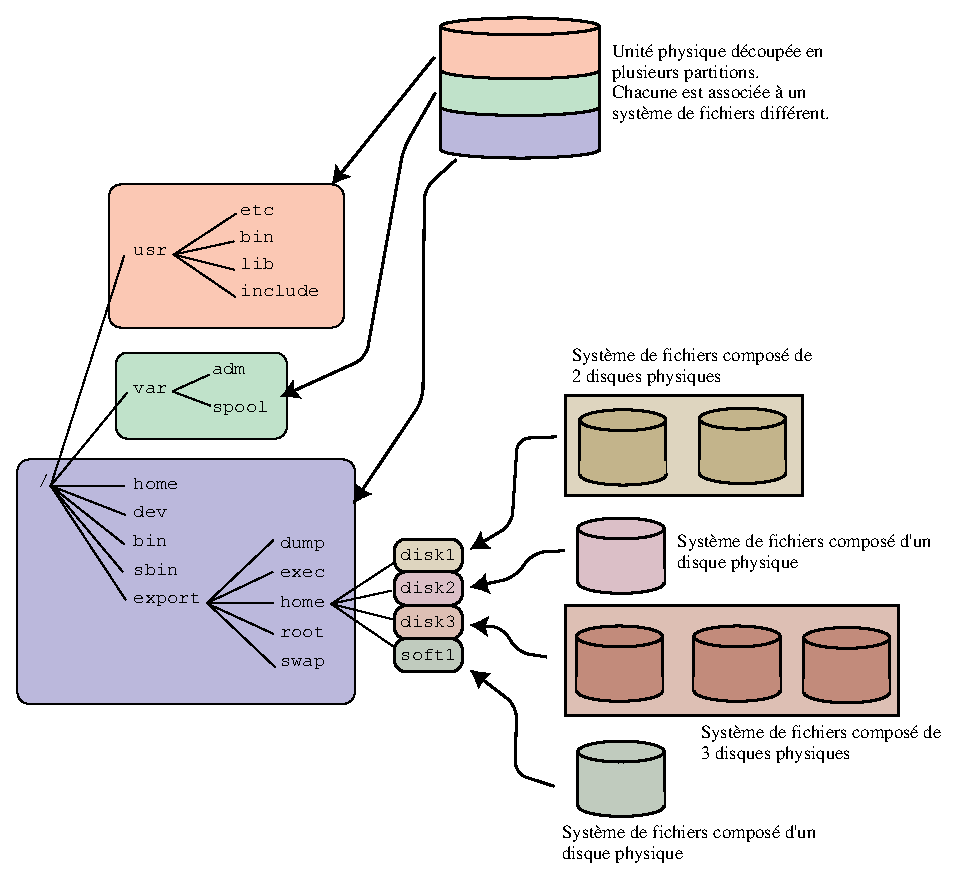
\includegraphics{./_Images/base-concepts/orgdisk}[l]
	\caption{\label{fig-bcpts-orgdisk}Organisation de l'arborescence {\Unix} avec les syst{\`e}mes de fichiers}
\end{figure}

Toutes les commandes {\Unix} distinguent les majuscules des
minuscules. Par exemple <<~{\tt ls}~>>, <<~{\tt Ls}~>> , <<~{\tt lS}~>>
et <<~{\tt LS}~>> sont quatre mots diff{\'e}rents au niveau de
l'interpr{\'e}teur de commandes.

Chaque commande {\Unix} est ex{\'e}cut{\'e}e dans un process
s{\'e}par{\'e}. Lorsqu'on tape une commande au niveau de
l'interpr{\'e}teur de commandes, celui-ci cr{\'e}e un sous processus dans
lequel il ex{\'e}cute la commande. Lorsque celle-ci est termin{\'e}e, le
sous process disparait en rendant la main au processus p{\`e}re.

%%%%%%%%%%%%%%%%%%%%%%%%%%%%%%%%%%%%%%%%%%%%%%%%%%%%%%%%%%%%%%%%%%%%%
\section{\label{bcpts-login}Connexion et d{\'e}connexion}

Comme tout syst{\`e}me multi-utilisateurs et multi-t{\^a}ches, {\Unix} associe
{\`a} chaque utilisateur~:
\begin{itemize}
	\item	un nom appel{\'e} \index{login@\textsl{login}}<<~{\sl login}~>>
			({\'e}quivalent au <<~{\sl Username}~>>.
			de {\OpenVMS}, ou au <<~{\sl logon name}~>> de {\WindowsNT})~;
	\item	un mot de passe~;
	\item	un num{\'e}ro d'utilisateur unique ou \index{UID}
			<<~{\sl UID}\footnote{{\sl UID}~=~User IDentifier}~>> ({\'e}quivalent
			{\`a} l'<<~{\sl UIC}~>> {\OpenVMS} ou <<~{\sl logon ID}~>> de
			{\WindowsNT}).
\end{itemize}

Par cons{\'e}quent, la premi{\`e}re chose que vous demandera le syst{\`e}me sera
votre <<~{\sl login}~>> et votre mot de passe. Si les deux sont valides,
{\Unix} initialisera votre environnement de travail.

\begin{remarque}
Pour des raisons de s{\'e}curit{\'e}, comme sous {\OpenVMS} et
{\WindowsNT}, {\Unix} ne verifie pas que le nom de <<~{\sl login}~>>
existe. Une fois que les deux informations seront saisies,
c'est-{\`a}-dire nom de <<~{\sl login}~>> et mot de passe, il ira
chercher dans la base des utilisateurs s'il existe un enregistrement et
un seul pour lesquelles ces deux informations sont exactes. Si cela,
n'est pas le cas, {\Unix} affichera le message d'erreur suivant~:
\begin{center}
\begin{verbatim}
Invalid login name.
\end{verbatim}
\end{center}
sans autre forme de renseignements.
\end{remarque}

En fonction du type de poste de travail, c'est-{\`a}-dire terminal passif ou
station de travail disposant d'un environnement graphique, la m{\'e}thode de
d{\'e}con\-nexion du syst{\`e}me varie.

Si votre environnement de travail est sur un terminal passif, la commande
de d{\'e}connexion est~:
\begin{quote}
\index{exit@\texttt{exit}}{\tt exit}
\end{quote}

Dans le cas des stations de travail graphiques, cela d{\'e}pend de l'interface
s{\'e}lectionn{\'e}e. En effet, il en existe plusieurs types dont~:
\begin{itemize}
	\item	<<~{\sl CDE}~>> ou <<~Common Desktop Environment~>>, environnement
			graphique d{\'e}velopp{\'e} {\`a} la base sur les stations Hewlett-Packard
			({\sl HP--VUE}) et r{\'e}pandue sur l'ensemble des {\Unix}s commerciaux
			comme {\sl Solaris}, {\sl Digital {\Unix}}, {\sf HP--UX},
			{\sf AIX}, {\sl Irix}, etc.
	\item	<<~{\sl fvwm95}~>>, environnement r{\'e}git par la <<~{\sl Free Software
			Foundation}~>> livr{\'e} de base avec {\Linux}, environnement
			dont la pr{\'e}sentation ressemble {\`a} {\Windows}95 (et sup{\'e}rieur)
			et {\WindowsNT} 4 (ou sup{\'e}rieur). Les sources de cet environnement
			sont disponibles et libres d'acc{\`e}s. Il est donc possible
			de les mettre sous n'importe quel plateforme {\Unix} (voire
			m{\^e}me {\OpenVMS}.
	\item	<<~{\sl KDE}~>>, environnement r{\'e}git par la <<~{\sl Free Software
			Foundation}~>> livr{\'e} de base avec {\Linux}, environnement
			dont la pr{\'e}sentation est un savant m{\'e}lange entre <<~{\sl CDE}~>>
			et l'<<~{\sl Active Desktop}~>> de {\sl Microsoft Corp.}.
	\item	<<~{\sl gnome}~>>, environnement r{\'e}git par la <<~{\sl Free Software
			Foundation}~>> livr{\'e} de base avec les futures versions de
			{\Linux}\footnote{RedHat Corp. pr{\'e}voit d'int{\'e}grer ce type
			d'interface en standard dans ces prochaines versions.},
			environnement orient{\'e} objet et int{\'e}grant roralement les ressources
			locales et distante sur le bureau.
	\item	<<~{\sl 4Dwm}~>>, environnement graphique disponible plus
			particuli{\`e}rement sur les stations {\sl Silicon Graphics Inc.}.
	\item	etc.
\end{itemize}

Il est clair que chaque interface dispose d'une boite de dialogue permettant
de terminer la session en cours. Nous de d{\'e}taillerons pas ici la m{\'e}thode
de d{\'e}connexion pour chacune de ces interfaces.

Comme tout syst{\`e}me o{\`u} un mot de passe est associ{\'e} {\`a} un utilisateur, il existe
une commande pour le changer. Sous {\Unix} cette commande est <<~{\tt passwd}~>>.
Elle vous demandera l'ancien mot de passe, le nouveau mot de passe puis une
confirmation.

{\bf En r{\'e}sum{\'e}~:}
\begin{quote}
\begin{tabular}{l@{\hspace{0.5cm}}p{6cm}}
	exit	&	D{\'e}connexion du syst{\`e}me.		\\[2ex]
	passwd	&	Changement du mot de passe.	\\[2ex]
\end{tabular}
\end{quote}

Le tableau \ref{tab-bcpts-login} donne un {\'e}quivalent entre les syst{\`e}mes
{\Unix} et{\OpenVMS} de {\sl Digital Equipment}.

\begin{table}[hbtp]
\centering
\begin{tabular}{|c|c|}
	\hline
	{\Unix}			&	{\OpenVMS}			\\
	\hline \hline
	{\tt exit}		&	{\tt LOGOUT}		\\
	{\tt passwd}	&	{\tt SET PASSWORD}	\\
	\hline
\end{tabular}
\caption{\label{tab-bcpts-login}\'{E}quivalences {\Unix} et {\OpenVMS}
pour la d{\'e}connexion et le changement de mot de passe.}
\end{table}

\begin{remarque}
Si vous tes connect  distance sur le systme {\Unix} grce  la
commande <<~\index{telnet@\texttt{telnet}}{\tt telnet}~>> (ou tout autre
type de protocole similaire comme <<~{\sf LAT}~>>, le comportement
obtenu est quivalent  celui d'un terminal passif.
\end{remarque}

%%%%%%%%%%%%%%%%%%%%%%%%%%%%%%%%%%%%%%%%%%%%%%%%%%%%%%%%%%%%%%%%%%%%%
\section{\label{bcpts-formcmd}Format d'une commande}

Une \index{commande!format}commande est constitu{\'e}e d'un nom suivi
d'arguments. Le s{\'e}parateur entre chaque mot d'une commande peut
{\^e}tre un ou plusieurs espaces ou tabulations.

\begin{definition}{Syntaxe}
\begin{verbatim}
% commande [options] [arguments] <CR>
\end{verbatim}
\end{definition}

\begin{example}
\begin{verbatim}
% banner HI
% ls -l shmoll lancelot DuLac
\end{verbatim}
\end{example}

\begin{remarque}
Sous {\Unix}, on fait la diff{\'e}rence entre majuscules et minuscules.
Par cons{\'e}quent {\tt ls}, {\tt Ls}, {\tt lS} et {\tt LS} sont quatres
termes diff{\'e}rents. De m{\^e}me, si on demande, par exemple, de taper <<~{\tt
q}~>>, il ne faudra pas taper <<~{\tt Q}~>>.
\end{remarque}


%%%%%%%%%%%%%%%%%%%%%%%%%%%%%%%%%%%%%%%%%%%%%%%%%%%%%%%%%%%%%%%%%%%%%
\section{Le manuel {\Unix}}

\subsection{Introduction, les sections}

Le \index{manuel!de r{\'e}f{\'e}rence}manuel de r{\'e}f{\'e}rence est
divis{\'e} en plusieurs sections. Chacune correspond {\`a} un sujet bien
particulier.

\begin{tabular}{l@{~:}p{8cm}}
	Section 1	& Les commandes utilisateur.\\
	Section 1m	& Les commandes d'administration syst{\`e}me.\\
	Section 2	& Les appels syst{\`e}mes (programmation).\\
	Section 3	& Les librairies de sous-routines (programmation).\\
	Section 4	& Les fichiers sp{\'e}ciaux.\\
	Section 5	& Les formats des fichiers.\\
	Section 6	& Liste des jeux.\\
	Section 7	& Possibilit{\'e}s diverses.\\
	Section 8	& Les commandes d'administration syst{\`e}me.\\
	Section 9	& Glossaire.
\end{tabular}

En g{\'e}n{\'e}ral, on retrouve dans la documentation papier la copie
conforme du manuel sur le syst{\`e}me. Il est bon de savoir la section
dans laquelle se trouve le manuel d'une commande. En effet, dans toute
documentation, les r{\'e}f{\'e}rences sont fournies sous le format
suivant~: <<~{\tt cmd (n)}~>> o{\`u} <<~{\tt cmd}~>> est le nom de la
commande et <<~{\tt n}~>> le num{\'e}ro de la section.

\subsection{Format d'une page du manuel}

Une page de \index{manuel!page du}manuel contient en g{\'e}n{\'e}ral les 11
parties suivantes~:
\begin{itemize}
	\item {\sl NAME}
	\item {\sl SYNOPSYS} (Syntaxe)
	\item {\sl HARDWARE DEPENDENCIES}
	\item {\sl EXAMPLES}
	\item {\sl FILES}
	\item {\sl RETURN VALUE}
	\item {\sl SEE ALSO}
	\item {\sl DIAGNOSTICS}
	\item {\sl BUGS}
	\item {\sl WARNINGS}
	\item {\sl AUTHOR}
\end{itemize}

Chacun de ces \index{manuel!paragraphes du}paragraphes d{\'e}crit les points suivants~:
\begin{description}
	\item[{\sl NAME}]\mbox{}\\
		Contient le nom de la commande ainsi qu'une description
		succincte. Le texte de cette section est utilis{\'e} pour  g{\'e}n{\'e}rer
		l'index g{\'e}n{\'e}ral.

	\item[{\sl SYNOPSYS}]\mbox{}\\
		Indique comment la commande est libell{\'e}e. Affiche en gras les
		caract{\`e}res tels qu'ils doivent {\^e}tre exactement frapp{\'e}s au terminal.
		Les termes entre crochets (<<~{\tt []}~>>) sont optionnels. Les champs
		r{\'e}guliers peuvent {\^e}tre remplis par des textes appropri{\'e}s. Les
		parenth{\`e}ses sont utilis{\'e}es pour montrer que l'argument pr{\'e}c{\'e}dent
		peut {\^e}tre r{\'e}p{\'e}t{\'e}. S'il y a doute sur la description de {\sl SYNOPSYS},
		lisez {\sl DESCRIPTION}.

	\item[{\sl DESCRIPTION}]\mbox{}\\
		Contient une description d{\'e}taill{\'e}e de ce que fait la commande.

	\item[{\sl HARDWARE DEPENDENCIES}]\mbox{}\\
		Signale les variantes d'exploitation selon le mat{\'e}riel.

	\item[{\sl EXAMPLES}]\mbox{}\\
		Certaines pages du manuel ont des exemples pas toujours limpides
		mais qui peuvent aider {\`a} mieux comprendre la commande.

	\item[{\sl FILES}]\mbox{}\\
		Tous les fichiers sp{\'e}ciaux que la commande utilise.

	\item[{\sl RETURN VALUE}]\mbox{}\\
		D{\'e}crit les valeurs en retour d'un appel programme.

	\item[{\sl SEE ALSO}]\mbox{}\\
		Renvoie {\`a} d'autres pages du manuel ou {\`a} une autre documentation
		pour de plus amples renseignements.

	\item[{\sl DIAGNOSTICS}]\mbox{}\\
		Si la commande fait ressortir des messages d'erreurs, ils sont
		explicit{\'e}s ici (en g{\'e}n{\'e}ral !!!).

	\item[{\sl BUGS}]\mbox{}\\
		D{\'e}crit les bugs (eh oui). Souvent utilis{\'e} pour vous pr{\'e}venir des
		probl{\`e}mes potentiels dans l'utilisation de cette commande.

	\item[{\sl WARNINGS}]\mbox{}\\
		idem que {\sl BUGS}.
\end{description}

\subsection{La commande {\tt man}}

La commande \index{man@\texttt{man}}<<~{\tt man}~>> recherche dans les
diff{\'e}rentes sections (1,2,3,4,5,6,7,8,9,1m) le mot clef. Elle
s'arr{\^e}te sur le premier mot clef trouv{\'e}. Ainsi, par exemple, on
verra syst{\'e}matiquement l'aide sur <<~{\tt passwd (1)}~>> par la
commande <<~{\tt man passwd}~>>; pour voir <<~{\tt passwd(4)}~>>, il
faudra taper la commande <<~{\tt man 4 passwd}~>>. Une fois trouv{\'e}e,
elle affiche le contenu d'un fichier d'aide {\`a} l'{\'e}cran en faisant
de la pagination. Celui-ci correspond {\`a} la page de manuel
associ{\'e}e.

\begin{tabular}{l@{~:~}l}
Pour passer {\`a} la ligne suivante & taper sur <<~\returnkey~>> \\
Pour passer {\`a} l'{\'e}cran suivant & taper sur <<~\spacekey~>> \\
Pour quitter & taper sur <<~\key{{\tt Q}}~>> ou <<~\key{{\tt q}}~>>
\end{tabular}

\begin{definition}{Syntaxe}
\begin{verbatim}
% man [n] commande
\end{verbatim}
O{\`u} l'option <<~{\tt n}~>> est le num{\'e}ro d'une section
\end{definition}

\begin{remarque}
Il est possible d'avoir une liste de commandes concern{\'e}es par un mot
clef de deux fa\c{c}ons~:

\begin{quote}
\verb=% man -k mot-clef= ({\tt k} comme {\sl keyword})
\end{quote}

ou bien

\begin{quote}
\verb=% apropos mot-clef=
\end{quote}

Ceci ne fonctionnera que si l'administrateur a constitu{\'e} la base de
donn{\'e}es r{\'e}f{\'e}ren\c{c}ant les mots clefs dans le manuel (fichier {\tt
whatis}).
\end{remarque}

\subsubsection{Equivalences}

Le tableau \ref{tab-equiv-man} donne un {\'e}quivalent entre les syst{\`e}mes
{\OpenVMS} de {\sl Digital Equipment}, {\DOS} et {\Unix}.

\begin{table}[hbtp]
\centering
\begin{tabular}{|c|c|c|}
	\hline
	{\Unix}		&	{\OpenVMS}		&	{\DOS} \\
	\hline \hline
	{\tt man}		&	{\tt HELP}		&	{\tt HELP}	\\
	{\tt apropos}	&	{\tt HELP}		&	{\tt HELP}	\\
	\hline
\end{tabular}
\caption{\label{tab-equiv-man}\'{E}quivalences {\OpenVMS},
{\DOS} et {\Unix} pour acc{\'e}der {\`a} l'aide}
\end{table}


%%%%%%%%%%%%%%%%%%%%%%%%%%%%%%%%%%%%%%%%%%%%%%%%%%%%%%%%%%%%%%%%%%%%%
\section{Introduction {\`a} la notion de {\sl file system}}

\subsection{Structure arborescente}

\index{fichier!nom de}Nous avons vu pr{\'e}c{\'e}demment qu'il n'y a plus de notions de
disques sous {\Unix}. Il en est de m{\^e}me pour les
p{\'e}riph{\'e}riques. De fa\c{c}on g{\'e}n{\'e}rale, tout est fichier.
On ne voit donc, au niveau utilisateur, qu'une seule arborescence
constitu{\'e}e de r{\'e}pertoires et de fichiers d{\'e}crivant les
ressources du syst{\`e}me (cf. figure \ref{fig-bc-struct-arb}). Le nom
d'un fichier sous {\Unix} est une suite de caract{\`e}res. Il n'existe
pas de notion de type de fichier et de num{\'e}ro de version comme sur
{\OpenVMS} ou {\DOS}. Le caract{\`e}re <<~{\tt .}~>> est
consid{\'e}r{\'e} comme {\'e}tant un caract{\`e}re dans le nom de
fichier et non pas, comme sur {\OpenVMS} ou {\DOS}, le caract{\`e}re de
s{\'e}paration entre le nom du fichier et son type. Il est donc possible
d'avoir un fichier dont le nom comporte plusieurs <<~{\tt .}~>>. La
philosophie des noms de fichiers ressemblerait donc {\`a} celle de
l'environnement {\MacOS}.

\begin{figure}[hbtp]
\centering
\setlength{\unitlength}{0.92pt}
\begin{picture}(359,151)
	\thinlines
	\put(260,47){\line(1,0){34}}	\put(299,43){fichier}
	\put(279,47){\line(0,-1){16}}	\put(299,27){fichier}
	\put(279,30){\line(1,0){16}}	\put(293,114){fichier}
	\put(272,117){\line(1,0){16}}	\put(293,98){fichier}
	\put(272,134){\line(0,-1){16}}	\put(198,12){fichier}
	\put(272,101){\line(1,0){16}}	\put(198,28){fichier}
	\put(272,118){\line(0,-1){16}}	\put(198,44){r{\'e}pertoire}
	\put(160,134){\line(1,0){124}}	\put(199,81){fichier}
	\put(177,32){\line(0,-1){16}}	\put(199,97){fichier}
	\put(177,15){\line(1,0){16}}	\put(289,129){r{\'e}pertoire}
	\put(158,48){\line(1,0){34}}	\put(95,17){fichier}
	\put(177,48){\line(0,-1){16}}	\put(95,70){fichier}
	\put(177,31){\line(1,0){16}}	\put(95,46){r{\'e}pertoire}
	\put(179,84){\line(1,0){16}}	\put(95,98){r{\'e}pertoire}
	\put(179,101){\line(0,-1){16}}	\put(95,131){r{\'e}pertoire}
	\put(160,101){\line(1,0){34}}	\put(10,132){{\tt /} (root)}
	\put(95,100){\line(-1,0){21}}	\put(95,73){\line(-1,0){21}}
	\put(95,49){\line(-1,0){21}}	\put(74,20){\line(0,1){115}}
	\put(96,20){\line(-1,0){21}}	\put(60,135){\line(1,0){32}}
\end{picture}
\caption{\label{fig-bc-struct-arb}Structure arborescente du syst{\`e}me {\Unix}}
\end{figure}

\begin{remarque}
Certains caract{\`e}res sont {\`a} {\'e}viter dans les noms de fichiers
tels que~:
\begin{itemize}
	\item l'espace~;
	\item la tabulation~;
	\item le caract{\`e}re <<~{\tt ;}~>>~;
	\item tout caract{\`e}re de contr{\^o}le (\esckey, \control{H}, \control{C},
		  etc.).
\end{itemize}
\end{remarque}

\begin{remarque}
Les noms de fichiers tiennent compte des majuscules/minuscules. Par
exemple~: <<~{\tt SIMPSONS}~>> et <<~{\tt simpsons}~>> sont deux
fichiers diff{\'e}rents.
\end{remarque}


\subsection{Les chemins d'acc{\`e}s}

\index{fichier!chemin d'acc{\`e}s {\`a} un}On distingue deux types de
chemins d'acc{\`e}s aux fichiers~:
\begin{itemize}
	\item les chemins d'acc{\`e}s absolus~;
	\item les chemins d'acc{\`e}s relatifs.
\end{itemize}

Les {\bf chemins d'acc{\`e}s absolus} sp{\'e}cifient un nom de fichier ou de
r{\'e}pertoire {\`a} partir de la racine. Les chemins d'acc{\`e}s absolus commencent
donc par <<~{\tt /}~>> qui est le nom de la racine ou du {\sl root directory}.

Les {\bf chemins d'acc{\`e}s relatifs} sp{\'e}cifient un nom de fichier ou de
r{\'e}pertoire {\`a} partir du r{\'e}pertoire courant, appel{\'e} aussi {\sl working
directory}. Par cons{\'e}quent, ces chemins ne commencent pas par <<~{\tt /}~>>
(exemple~: {\tt dir/essai}).

\begin{definition}{En r{\'e}sum{\'e}}
\index{chemin d'acc{\`e}s!absolu}Chemins d'acc{\`e}s absolus~:\\[0.5ex]
\begin{itemize}
	\item Commencent par <<~{\tt /}~>>~;
	\item Repr{\'e}sentent la position relative par rapport au {\sl root directory}.
\end{itemize}

\index{chemin d'acc{\`e}s!relatif}Chemins d'acc{\`e}s relatifs~:\\[0.5ex]
\begin{itemize}
	\item Ne commencent pas par <<~{\tt /}~>>,
	\item Repr{\'e}sentent la position relative par rapport au r{\'e}pertoire courant.
\end{itemize}
\end{definition}

\begin{example}
\begin{tabular}{|l|l|l|l|}
	\hline
		\multicolumn{1}{|c|}{syst{\`e}me}				&
		\multicolumn{1}{|c|}{d{\'e}placement relatif}	&
		\multicolumn{1}{|c|}{d{\'e}placement absolu}	\\
	\hline
		{\Unix}						&
		\verb=cd ../repertoire=			&
		\verb=cd /home/users/schmoll= 	\\
	\hline
		{\OpenVMS}							&
		\verb=set default [-.repertoire]= 		&
		\verb=set default disk$users:[schmoll]=	\\
	\hline
		{\DOS}				&
		\verb=CD ..\REPERT=			&
		\verb=CD C:\USERS\SCHMOLL=	\\
	\hline
\end{tabular}
\end{example}

\subsection{Principaux r{\'e}pertoires {\Unix}}

\index{r{\'e}pertoire!syst{\`e}me}
\begin{description}
	\item[{\sl Root directory (<<~{\tt /}~>>)}]\mbox{}\\
		C'est le haut de l'arborescence. Il n'y a qu'une et une seule entr{\'e}e sur
		le file system. Le {\sl root directory} est le seul r{\'e}pertoire sans p{\`e}re.
		Tous les fichiers et chemins d'acc{\`e}s absolus ont le {\sl root directory}
		dans le chemin d'acc{\`e}s.

	\item[{\sl R{\'e}pertoires {\tt /bin} et {\tt /sbin}}]\mbox{}\\
		Les r{\'e}pertoires {\tt /bin} et {\tt /sbin} contiennent les commandes de base
		{\Unix} de la section 1 ({\tt ls}, {\tt cp}, {\tt rm}, {\tt mv},
		{\tt ln}, etc.) utilis{\'e}es entre autre lors du d{\'e}marrage du syst{\`e}me.
		Les fichiers contenus dans ces r{\'e}pertoires ne sont que des ex{\'e}cutables.

	\item[{\sl R{\'e}pertoire {\tt /dev}}]\mbox{}\\
		Le r{\'e}pertoire {\tt /dev} contient les
		\index{fichier!sp{\'e}cial}fichiers sp{\'e}ciaux permettant de
		communiquer avec tous les p{\'e}riph{\'e}riques comme les disques, les
		terminaux, les d{\'e}rouleurs de bandes, les imprimantes, etc.

	\item[{\sl R{\'e}pertoire {\tt /etc}}]\mbox{}\\
		Le r{\'e}pertoire {\tt /etc} contient tous les fichiers d'administration et
		un certain nombre de commandes syst{\`e}me. Le r{\'e}pertoire {\tt /etc} porte
		bien son nom\footnote{{\tt etc} a vraiment {\'e}t{\'e} choisi pour la
		signification de {\sl et caetera}}.

       \item[{\sl R{\'e}pertoires {\tt /home} et {\tt /root}}]\mbox{}\\
                Le r{\'e}pertoire {\tt /home} contient les r\'epertoires personnels des utilisateurs du syst\`eme.\\
		Le r{\'e}pertoire {\tt /root} est le r\'epertoire personnel de l'administrateur.

	\item[{\sl R{\'e}pertoire {\tt /usr} et sous-r{\'e}pertoires}]\mbox{}\\
		Le r{\'e}pertoire {\tt /usr} contient un certain nombre de sous-r{\'e}pertoires.
		Chacun contient les fichiers n{\'e}cessaires au fonctionnement en mode normal
		du syst{\`e}me\footnote{mode multi-utilisateurs}. Par exemple~:
		\begin{itemize}
			\item {\tt /usr/bin} et {\tt /usr/sbin} contiennent les commandes
			suppl{\'e}mentaires non contenues dans {\tt /bin} et {\tt /sbin}~;
			\item {\tt /usr/lib} contient les biblioth{\`e}ques pour le fonctionnement
			d'{\Unix} et pour le d{\'e}veloppement~;
			\item {\tt /usr/include} contient les fichiers de d{\'e}claration des
			fonctions syst{\`e}me pour le d{\'e}veloppement.
		\end{itemize}

        \item[{\sl R{\'e}pertoire {\tt /var}}]\mbox{}\\
                Le r{\'e}pertoire {\tt /var} contient les fichiers variables (succeptibles d'\^etre modifi\'es fr\'equemment) : journaux (logs), e-mails, bases de donn\'ees, archives, \ldots
\end{description}


%%%%%%%%%%%%%%%%%%%%%%%%%%%%%%%%%%%%%%%%%%%%%%%%%%%%%%%%%%%%%%%%%%%%%
\section{Les entr{\'e}es/sorties}

A chaque cr{\'e}ation de processus, celui ci se voit affect{\'e} trois canaux de
communication~:
\begin{itemize}
	\item l'entr{\'e}e standard~;
	\item la sortie standard~;
	\item la sortie d'erreurs standard.
\end{itemize}

La figure \ref{fig-bcpts-iochans} illustre les trois canaux de communications
que poss{\`e}de chaque processus sur le syst{\`e}me {\Unix}.

\begin{figure}[hbtp]
\centering
\epsfbox{_Images/base-concepts/iochans.eps}
%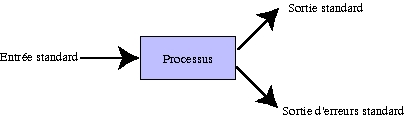
\includegraphics{./_Images/base-concepts/iochans.jpg}
\caption{\label{fig-bcpts-iochans}Entr{\'e}es/Sorties d'un processus}
\end{figure}


Chacun des trois canaux se voit affecter un nom de fichier et un num{\'e}ro~:

\begin{tabular}{|l|c|c|}
	\hline
		\multicolumn{1}{|c|}{Canal de communication}		&
		\multicolumn{1}{|c|}{Fichier}						&
		\multicolumn{1}{|c|}{Num{\'e}ro logique}			\\
	\hline \hline
		Entr{\'e}e standard			&
		{\tt stdin}					&
		0							\\
	\hline
		Sortie standard				&
		{\tt stdout}				&
		1							\\
	\hline
		Sortie d'erreurs standard	&
		{\tt stderr}				&
		2							\\
	\hline
\end{tabular}

Le fichier \index{stdin@\texttt{stdin} (entr{\'e}e standard)}{\tt stdin} ({\sl entr{\'e}e standard}), est le fichier {\`a} partir duquel
le process va lire les donn{\'e}es n{\'e}cessaires en entr{\'e}e. Il est ouvert avec
le num{\'e}ro logique 0({\sl file descriptor C}), et il est, par d{\'e}faut associ{\'e}
au clavier.

Le fichier \index{stdout@\texttt{stdout} (sortie standard)}{\tt stdout} ({\sl sortie standard}), est le fichier dans
lequel le process va {\'e}crire les messages qu'il produit en sortie, dans
le cas d'une ex{\'e}cution normale. Il est ouvert avec le num{\'e}ro logique 1
({\sl file descriptor C}), et il est, par d{\'e}faut associ{\'e} {\`a} l'{\'e}cran.

Le fichier \index{stderr@\texttt{stderr} (sortie d'erreurs standard)}{\tt stderr} ({\sl sortie d'erreurs standard}), est le
fichier dans lequel le process va {\'e}crire les messages d'erreur. Il est
ouvert avec le num{\'e}ro logique 2 ({\sl file descriptor C}), et il est par
d{\'e}faut associ{\'e} {\`a} l'{\'e}cran.

\begin{remarque}
On distingue toujours deux canaux de sorties (un pour les sorties
normales et un pour les erreurs). En effet, si un process doit {\'e}crire
dans un fichier et qu'une erreur se produit (impossibilit{\'e} d'{\'e}crire par
exemple), il faut afficher un message sur un canal de sortie diff{\'e}rent.
\end{remarque}

Le tableau \ref{tab-bcpts-equiv-iochans} donne les {\'e}quivalences des noms
des canaux d'entr{\'e}es/sorties entre les syst{\`e}mes {\Unix} et {\OpenVMS} de Digital.

\begin{table}[hbtp]
\centering
\begin{tabular}{|l|c|c|}
	\hline
		{\Unix}	&	{\OpenVMS}	\\
	\hline \hline
		{\tt stdin}		&	\verb=SYS$INPUT=	\\
		{\tt stdout}	&	\verb=SYS$OUTPUT=	\\
		{\tt stderr}	&	\verb=SYS$ERROR=	\\
	\hline
\end{tabular}
\caption{\label{tab-bcpts-equiv-iochans}\'{E}quivalences des noms
des canaux d'entr{\'e}es/sorties entre {\Unix} et {\OpenVMS}}
\end{table}


%%%%%%%%%%%%%%%%%%%%%%%%%%%%%%%%%%%%%%%%%%%%%%%%%%%%%%%%%%%%%%%%%%%%%
\section{\label{bcpts-filters}Les filtres}

\index{filtre}Un filtre est une commande {\Unix} devant effectuer une action sur
les donn{\'e}es en lecture {\`a} partir de l'entr{\'e}e standard et afficher le
r{\'e}sultat en {\'e}criture sur la sortie standard.

La figure \ref{fig-bcpts-filters-desc} montre le principe des filtres sous
{\Unix}.

\begin{figure}[hbtp]
\centering
\epsfbox{_Images/base-concepts/filters-desc.eps}
%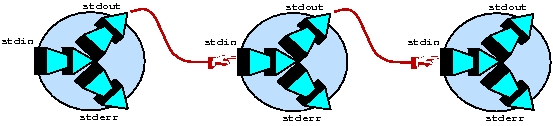
\includegraphics{./_Images/base-concepts/filters-desc.jpg}
\caption{\label{fig-bcpts-filters-desc}Principe des filtres sous {\Unix}}
\end{figure}

Il est possible d'encha{\^\i}ner plusieurs filtres les uns aux autres. Par
contre, les process en d{\'e}but et en fin de cha{\^\i}nes ne doivent pas se
comporter comme des filtres.

	%% Ok, index

%%%%%%%%%%%%%%%%%%%%%%%%%%%%%%%%%%%%%%%%%%%%%%%%%%%%%%%%%%%%%%%%%%%%%%%%
%                                                                      %
% This program is free software; you can redistribute it and/or modify %
% it under the terms of the GNU General Public License as published by %
% the Free Software Foundation; either version 2 of the License, or    %
% (at your option) any later version.                                  %
%                                                                      %
% This program is distributed in the hope that it will be useful,      %
% but WITHOUT ANY WARRANTY; without even the implied warranty of       %
% MERCHANTABILITY or FITNESS FOR A PARTICULAR PURPOSE.  See the        %
% GNU General Public License for more details.                         %
%                                                                      %
% You should have received a copy of the GNU General Public License    %
% along with this program; if not, write to the Free Software          %
% Foundation, Inc., 51 Franklin St, Fifth Floor, Boston,               %
% MA  02110-1301  USA                                                  %
%                                                                      %
%%%%%%%%%%%%%%%%%%%%%%%%%%%%%%%%%%%%%%%%%%%%%%%%%%%%%%%%%%%%%%%%%%%%%%%%
%
%	$Id$
%

\setcounter{remarque-cnt}{1}
\setcounter{example-cnt}{1}
\chapter{Commandes {\Unix}}

%%%%%%%%%%%%%%%%%%%%%%%%%%%%%%%%%%%%%%%%
\section{Commandes li{\'e}es au file system}

\subsection{\label{cmds-pwd-cd}Commandes {\tt pwd} et {\tt cd}}

\begin{tabular}{c@{~=~}l}
	\index{pwd@\texttt{pwd}}{\tt pwd}	&	Print Working Directory \\
	\index{cd@\texttt{cd}}{\tt cd}		&	Change Directory \\
\end{tabular}

\begin{definition}{Syntaxe}
\begin{tabular}{lp{8cm}}
	{\tt pwd}			&	Affiche le chemin d'acc{\`e}s absolu du r{\'e}pertoire
							courant.\\
	{\tt cd repertoire}	&	Change le r{\'e}pertoire courrant.\\
\end{tabular}
\end{definition}

\begin{example}
\begin{quote}
\begin{verbatim}
% pwd
/home/users/bart
% cd /home/users/schmoll
\end{verbatim}
\end{quote}
\end{example}

Le tableau \ref{tab-cmds-pwdcd} donne une {\'e}quivalence des commandes de
d{\'e}placement dans l'arborescence entre {\Unix} et {\OpenVMS}
\index{pwd@\texttt{pwd}!{\'e}quivalence}\index{cd@\texttt{cd}!{\'e}quivalence}.

\begin{table}[hbtp]
\centering
\begin{tabular}{|l|l|}
	\hline
	{\Unix}	&	{\OpenVMS}		\\
	\hline \hline
	{\tt cd}	&	{\tt SET DEFAULT}	\\
	\hline
	{\tt pwd}	&	{\tt SHOW DEFAULT}	\\
	\hline
\end{tabular}
\caption{\label{tab-cmds-pwdcd}\'{E}quivalence des commandes de d{\'e}placement
dans l'arborescence sur le syst{\`e}me}
\end{table}


\subsection{\label{cmds-unix-ls}Commande {\tt ls}}

\begin{definition}{Syntaxe}
\begin{verbatim}
ls [-ladFR] [fichier ...]
\end{verbatim}
Liste le contenu d'un r{\'e}pertoire.
\end{definition}

\index{ls@\texttt{ls}}La commande "{\tt ls}" sans argument, liste les noms de fichiers (ou
de r{\'e}pertoires) pr{\'e}sents dans le r{\'e}pertoire courant. Cette commande,
utilis{\'e}e avec un nom de fichier comme argument, permettra de v{\'e}rifier
l'existence de celui-ci. Si l'argument utilis{\'e} est un nom de r{\'e}pertoire,
"{\tt ls}" en listera le contenu.

\index{ls@\texttt{ls}!options}Il existe de tr{\`e}s nombreuses options pour la commande "{\tt ls}".
La liste ci-dessous est les options les plus utilis{\'e}es.\\
\begin{tabular}{lp{10cm}}
	{\tt -l}	&
		affiche le type de fichier, les protections, le nombre de liens avec le
		fichier, le propri{\'e}taire, le groupe, la taille en octets, la date de
		derni{\`e}re modification et le nom du fichier.\\
	{\tt -F}	&
		ajoute un "{\tt /}" apr{\`e}s le nom de chaque r{\'e}pertoire,
		un "{\tt *}" apr{\`e}s chaque fichier poss{\'e}dant le 
		droit d'ex{\'e}cution et un "{\tt @}" apr{\`e}s chaque fichier lien (cf.
		section \ref{cmds-cpmvln}).\\
	{\tt -a}	&
		liste tous les fichiers y compris les fichiers cach{\'e}s.\\
	{\tt -R}	&
		liste les fichiers et les r{\'e}pertoires de fa\c{c}on r{\'e}cursive.\\
	{\tt -d}	&
		ne descend pas dans un r{\'e}pertoire si le param{\`e}tre est un nom de r{\'e}pertoire.
\end{tabular}

\begin{example}
\begin{verbatim}
% ls -F
dir1/ fic1 fic2* fic3@
% ls -a
. .. .profile dir1 fic1 fic2 fic3
% ls -l
drw-rw-rw- 3 schmoll esme 24 Jul 25 10:00 dir2
-rw-r--r-- 1 schmoll esme 37 Jul 25 12:00 fic1
-rwxr-xr-x 1 schmoll esme 37 Jul 25 12:00 fic2
lrw-r--r-- 1 schmoll esme 37 Jul 25 12:00 fic3 -> /tmp/ficref
% ls -R
dir1 fic1 fic2 fic3
./dir1:
fic4 fic5
% ls -d dir1
dir1
\end{verbatim}
\end{example}

\index{ls@\texttt{ls}!{\'e}quivalence}Le tableau \ref{tab-cmds-dir} montre les
{\'e}quivalences entre les commandes des syst{\`e}mes {\Unix},
{\OpenVMS} et {\DOS} pour afficher la liste des fichiers d'un
r{\'e}pertoire.

\begin{table}[hbtp]
\centering
\begin{tabular}{|l|l|l|}
	\hline
		\multicolumn{1}{|c|}{\Unix}		&
		\multicolumn{1}{|c|}{\OpenVMS}	&
		\multicolumn{1}{|c|}{\DOS}		\\
	\hline \hline
	{\tt ls}		&	{\tt DIRECTORY}			&	{\tt DIR}							\\
	{\tt ls -l}		&	{\tt DIRECTORY/FULL}	&	{\it N/A}							\\
	{\tt ls -R}		&	{\tt DIRECTORY [...]}	&	{\it Absent de {\tt COMMAND.COM}}	\\
	{\tt ls rep}	&	{\tt DIRECTORY [.REP]}	&	\verb=DIR \REP=						\\
	{\tt ls -d rep}	&	{\tt DIRECTORY REP.DIR}	&	{\tt DIR REP}						\\
	\hline
\end{tabular}
\caption{\label{tab-cmds-dir}\'{E}quivalences entre syst{\`e}mes pour
afficher la liste des fichiers d'un r{\'e}pertoire}
\end{table}

\subsection{Commandes {\tt mkdir} et {\tt rmdir}}

\begin{definition}{Syntaxe}
\begin{tabular}{ll}
	\index{mkdir@\texttt{mkdir}}\verb=mkdir [-p] directory ...=	& (make directory) \\
	\index{rmdir@\texttt{rmdir}}\verb=rmdir directory ...=		& (remove directory)\\
\end{tabular}
\end{definition}

La commande {\tt mkdir} permet de cr{\'e}er des r{\'e}pertoires. Lorsqu'un
r{\'e}pertoire est cr{\'e}{\'e}, il poss{\`e}de automatiquement deux sous r{\'e}pertoires~:
"{\tt .}" et "{\tt ..}" qui seront examin{\'e}s plus loin. La commande
{\tt rmdir} permet de supprimer des r{\'e}pertoires. Les r{\'e}pertoires {\`a} supprimer
doivent imp{\'e}rativement {\^e}tre vides (ils ne doivent contenir que les
r{\'e}pertoires "{\tt .}" et "{\tt ..}"). D'autre part, il est
impossible de supprimer des r{\'e}pertoires qui se trouvent entre la racine
et le r{\'e}pertoire courant. Chacune de ces deux commandes peut avoir
plusieurs arguments. Les arguments de {\tt mkdir} sont les noms de r{\'e}pertoires
{\`a} cr{\'e}er. Les arguments de {\tt rmdir} doivent {\^e}tre des noms de r{\'e}pertoires
d{\'e}j{\`a} existants. Dans les deux cas, on peut utiliser des chemins d'acc{\`e}s
relatifs ou absolus.

\begin{remarque}
Lorsqu'on utilise la commande {\tt rmdir} avec plusieurs arguments, {\tt
rmdir} d{\'e}truit les r{\'e}pertoires dans l'ordre dans lequel ils ont {\'e}t{\'e}
pr{\'e}cis{\'e}s sur la ligne de commande. Par cons{\'e}quent, si l'on veut en
d{\'e}truire plusieurs, l'ordre sur la ligne de commande a une importance.
\end{remarque}

\begin{example}
\begin{verbatim}
% mkdir mondir
% mkdir mondir/sd1 mondir/sd2 mondir/sd1/sd11
% mkdir mondir/sd3/sd31
% rmdir mondir/sd2
% rmdir mondir/sd3/sd31 mondir/sd3
% rmdir mondir/sd1/sd11 mondir/sd1 mondir
\end{verbatim}
\end{example}

\index{mkdir@\texttt{mkdir}!{\'e}quivalence}\index{rmdir@\texttt{rmdir}!{\'e}quivalence}Le
tableau \ref{tab-cmds-mkdir} montre les {\'e}quivalences entre les
commandes des syst{\`e}mes {\Unix}, {\OpenVMS} et {\DOS} pour la gestion
des r{\'e}pertoires.

\begin{table}[hbtp]
\centering
\begin{tabular}{|l|l|l|}
	\hline \centering
	{\Unix}		&	{\OpenVMS}				&	{\DOS}			\\
	\hline \hline
	{\tt mkdir}	&	{\tt CREATE/DIRECTORY}	&	{\tt MD} ou {\tt MKDIR}	\\
	{\tt rmdir}	&	{\tt DELETE}			&	{\tt RD} ou {\tt RMDIR}	\\
	\hline
\end{tabular}
\caption{\label{tab-cmds-mkdir}\'{E}quivalences entre syst{\`e}mes pour la gestion
des r{\'e}pertoires}
\end{table}

%%%%%%%%%%%%
\subsection{R{\'e}pertoires "{\tt .}" et "{\tt ..}"}

\index{r{\'e}pertoire!"\texttt{.}"}\index{r{\'e}pertoire!"\texttt{..}"}
Quand un r{\'e}pertoire est cr{\'e}{\'e}, le syst{\`e}me g{\'e}n{\`e}re
automatiquement deux sous-r{\'e}pertoires repr{\'e}sentant des liens
vers le r{\'e}pertoire cr{\'e}{\'e} et le r{\'e}pertoire p{\`e}re~:
\begin{itemize}
	\item	le r{\'e}pertoire "{\tt .}"= r{\'e}pertoire courant,
	\item	le r{\'e}pertoire "{\tt ..}" = r{\'e}pertoire p{\`e}re.
\end{itemize}

Le r{\'e}pertoire "{\tt ..}" est tr{\`e}s utile pour r{\'e}f{\'e}rencer ce qui se
trouve au dessus du r{\'e}pertoire courant dans l'arborescence du file
system. Ainsi il suffira d'utiliser "{\tt ..}" dans un chemin d'acc{\`e}s
relatif pour r{\'e}f{\'e}rencer le r{\'e}pertoire p{\`e}re.

Par exemple "{\tt cd ..}" remonte d'un cran dans l'arborescence et
"{\tt more ../../fic}" liste le contenu d'un fichier deux niveaux au
dessus dans l'arborescence. La figure \ref{fig-cmds-dotdirs} montre les
liens entre les r{\'e}pertoires "{\tt .}" et "{\tt ..}" et les r{\'e}pertoires
fils et p{\`e}res.

\begin{figure}[hbtp]
\centering
%\epsfbox{_Images/cmds-unix/dotdirs.eps}
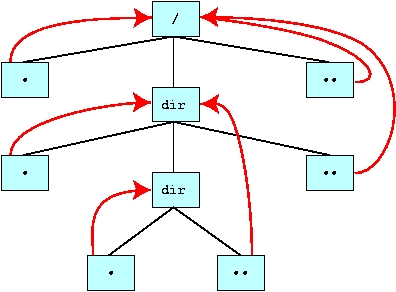
\includegraphics{./_Images/cmds-unix/dotdirs.jpg}
\caption{\label{fig-cmds-dotdirs}Liens des r{\'e}pertoires "{\tt .}" et
"{\tt ..}"}
\end{figure}

Le tableau \ref{tab-cmds-dotdirs} montre des exemples d'{\'e}quivalences
entre les syst{\`e}mes {\Unix}, {\OpenVMS} et {\DOS} de manipulation des
r{\'e}pertoires "{\tt .}" et "{\tt ..}".

\begin{table}[hbtp]
\centering
\begin{tabular}{|l|l|l|}
	\hline
	{\Unix}		&	{\OpenVMS}	&	{\DOS}	\\
	\hline \hline
	{\tt .}		&	{\tt []}	&	{\tt .}			\\
	{\tt ..}	&	{\tt [-]}	&	{\tt ..}		\\
	{\tt ../..}	&	{\tt [--]}	&	\verb=..\..=	\\
	\hline
\end{tabular}
\caption{\label{tab-cmds-dotdirs}Exemples d'equivalences entre syst{\`e}mes pour
la manipulation des r{\'e}pertoires "{\tt .}" et "{\tt ..}"}
\end{table}
	
%%%%%%%%%%%%%%%%%%%%%%%%%%%%%%%%%%%%%%%%
\section{Commandes de manipulation de fichiers}

\subsection{Attributs d'un fichier}

\index{fichier!attributs}Par d{\'e}finition, un fichier est une suite d'octets poss{\'e}dant les
attributs suivants~:
\begin{itemize}
	\item	un type,
	\item	un masque de protection,
	\item	un nombre de liens avec d'autres fichiers,
	\item	un propri{\'e}taire et groupe,
	\item	une taille,
	\item	une date de cr{\'e}ation et de derni{\`e}re modification,
	\item	un nom.
\end{itemize}

Les diff{\'e}rents types de fichiers sont~:
\begin{center}
\begin{tabular}{|l|c|}
	\hline
	\multicolumn{1}{|c|}{type}				&	code	\\
	\hline \hline
	standard								&	{\tt -}	\\
	r{\'e}pertoire							&	{\tt d}	\\
	lien symbolique							&	{\tt l}	\\
	fichier sp{\'e}cial mode block			&	{\tt b}	\\
	fichier sp{\'e}cial mode caract{\`e}re	&	{\tt c}	\\
	fichier sp{\'e}cial mode r{\'e}seau		&	{\tt n}	\\
	pipe nomm{\'e}							&	{\tt p}	\\
	\hline
\end{tabular}
\end{center}

Le type "lien symbolique" correspond {\`a} un \index{fichier!lien
symbolique}fichier sp{\'e}cial pointant physiquement sur un autre.

Les types \index{fichier!sp{\'e}cial}"fichier sp{\'e}cial mode
block" et "fichier sp{\'e}cial mode caract{\`e}re" servent {\`a}
communiquer avec les p{\'e}riph{\'e}riques (disques, terminaux, etc.).

Le type "fichier sp{\'e}cial mode r{\'e}seau" sert de canal de communication
entre processes sur diff{\'e}rentes machines.

Le type "pipe nomm{\'e}" sert de canal de communication entre diff{\'e}rents
processes sur une m{\^e}me machine.

%%%%%%%%%%%%
\subsection{Affichage du contenu d'un fichier - Commandes {\tt cat} et
{\tt more}}

\begin{definition}{Syntaxe}
\begin{verbatim}
cat fichier...
more fichier...
\end{verbatim}
\end{definition}

La commande \index{cat@\texttt{cat}}{\tt cat} concat{\`e}ne le contenu des fichiers en arguments et
affiche le contenu sur la sortie standard.

La commande \index{more@\texttt{more}}{\tt more} visualise le contenu des fichiers page {\'e}cran par
page {\'e}cran. Pour visualiser la page suivante, il suffit de frapper sur
\spacekey, ou de frapper sur \returnkey
afin de visualiser une ligne suppl{\'e}mentaire. Pour terminer la
visualisation avant la fin du fichier, taper sur la touche "{\tt Q}"
ou "{\tt q}". D'autres commandes sont disponibles, pour cela taper sur
la touche "{\tt h}" ou "{\tt H}" lorsque more a termin{\'e} d'afficher
une page {\'e}cran.

Le tableau \ref{tab-cmds-catmore} montre l'{\'e}quivalence entre les commandes {\tt cat}
et {\tt more} et d'autres syst{\`e}mes ({\OpenVMS} et {\DOS}).

\begin{table}
\centering
\begin{tabular}{|l|l|l|}
	\hline
	\multicolumn{1}{|c|}{{\Unix}}		&
	\multicolumn{1}{|c|}{{\OpenVMS}}	&
	\multicolumn{1}{|c|}{{\DOS}}			\\
	\hline \hline
	{\tt cat}		&	{\tt type}		&	{\tt TYPE}				\\
	{\tt more}		&	{\tt type/page}	&	{\tt TYPE ... | MORE}	\\
	\hline
\end{tabular}
\caption{\label{tab-cmds-catmore}\'{E}quivalence entre {\tt cat}et {\tt
more} et d'autres syst{\`e}mes}
\end{table}

%%%%%%%%%%%
\subsection{\label{cmds-cpmvln}Manipulation de fichiers - Commandes {\tt cp}, {\tt mv} et {\tt ln}}

\begin{definition}{D{\'e}finition}
\begin{tabular}{lp{8cm}}
	{\tt cp}	&	copie les fichiers. \\
	{\tt mv}	&	renomme les fichiers et r{\'e}pertoires et/ou
					d{\'e}place les fichiers. \\
	{\tt ln}	&	cr{\'e}e un lien sur un fichier ou un r{\'e}pertoire.
\end{tabular}
\end{definition}

\begin{definition}{Syntaxe}
{\tt cp [-i] fichier-source} $\cdots$ {\tt destination}\\
{\tt mv [-i] fichier-source} $\cdots$ {\tt destination}\\
{\tt ln [-s] fichier-source lien-destination}
\end{definition}

\index{cp@\texttt{cp}}Lorsque le commande "{\tt cp}" ne poss{\`e}de que deux ("{\tt cp fichier1
fichier2}"), elle effectue une copie du fichier source vers le fichier
destination. Si celui-ci existait d{\'e}j{\`a} il est supprim{\'e} pour {\^e}tre
remplacer par le nouveau.

Lorsque la commande "{\tt cp}" poss{\`e}de plus de deux arguments
(plusieurs fichiers source), la destination est obligatoirement un
r{\'e}pertoire ("{\tt cp fichier1 fichier2 repertoire}"). Dans ce cas,
elle duplique ces fichiers dans le r{\'e}pertoire sp{\'e}cifi{\'e}. S'il en existait
d{\'e}j{\`a} sous le m{\^e}me nom , ils sont supprim{\'e}s pour {\^e}tre remplac{\'e} par les
copies.

\index{mv@\texttt{mv}}La commande "{\tt mv}" r{\'e}agit de fa\c{c}on similaire~:
\begin{itemize}
	\item	si elle ne poss{\`e}de que deux arguments, elle renomme le fichier
			source sous le nouveau nom,
	\item	si elle poss{\`e}de plusieurs arguments, la destination est
			obligatoirement un r{\'e}pertoire. Dans ce cas, elle d{\'e}place les
			fichiers sources dans le r{\'e}pertoire sp{\'e}cifi{\'e}.
\end{itemize}

De m{\^e}me, si des fichiers existaient d{\'e}j{\`a} sous le m{\^e}me nom, ils seront
supprim{\'e}s. Dans le cas particulier o{\`u} la commande "{\tt mv}" ne
poss{\`e}de que deux arguments et que la destination est un nom de
r{\'e}pertoire, le fichier source est d{\'e}plac{\'e} {\`a} ce nouveau point de
l'arborescence.

Les fichiers source de la commande "{\tt cp}" ne peuvent pas {\^e}tre des
r{\'e}pertoires.

Les fichiers source de la commande "{\tt mv}" peuvent {\^e}tre de
n'importe quel type.

\index{ln@\texttt{ln}}La commande "{\tt ln}" autorise l'acc{\`e}s
{\`a} un fichier via plusieurs noms, ce sont des cr{\'e}ations de liens
entre fichiers. La syntaxe est~:
\begin{quote}
\begin{center}
{\tt ln fichier1 fichier2}
\end{center}
\begin{itemize}
	\item {\tt fichier1} qui existe d{\'e}j{\`a}, va pouvoir {\^e}tre acc{\'e}d{\'e} via 
		le nouveau nom {\tt fichier2}. 
	\item {\tt fichier2} est alors li{\'e} avec {\tt fichier1}.
\end{itemize}
\end{quote}

\index{fichier!lien symbolique}On distingue deux types de liens~: les liens symboliques et les liens logiques.

\begin{itemize}
	\item	\index{lien!symbolique}Dans le cas du lien symbolique, {\tt fichier2} (fichier lien)
			pointe sur {\tt fichier1} (fichier source) permettant d'acc{\'e}der
			aux informations sur le disque. Par cons{\'e}quent, si {\tt fichier1}
			est effac{\'e}, le contenu est perdu et {\tt fichier2} pointe 
			sur quelque chose d'inexistant. {\bf L'information est donc perdue}.\\
	\item	\index{lien!logique}Dans le cas du lien logique, {\tt fichier1} (fichier source) et
			{\tt fichier2} (fichier lien) pointent directement sur les donn{\'e}es
			r{\'e}sidant sur le disque. Par cons{\'e}quent,si {\tt fichier1} est effac{\'e},
			{\bf le contenu n'est pas perdu et est toujours accessible par 
			{\tt fichier2}}.
\end{itemize}

La figure \ref{fig-cmds-links} montre les diff{\'e}rences entre les liens symboliques
et les liens logiques vis {\`a} vis de leur liaisons avec les informations sur
le syst{\`e}me de fichiers.

\begin{figure}[hbtp]
\centering
%\epsfbox{_Images/cmds-unix/log-links.eps}
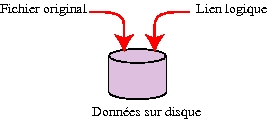
\includegraphics{./_Images/cmds-unix/log-links.jpg}
%\epsfbox{_Images/cmds-unix/symb-links.eps}
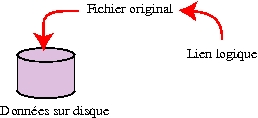
\includegraphics{./_Images/cmds-unix/symb-links.jpg}
\caption{\label{fig-cmds-links}Diff{\'e}rence entre les liens symboliques et les
liens logiques}
\end{figure}

\begin{remarque}
Deux ou plusieurs fichiers li{\'e}s par un lien logique doivent r{\'e}sider
sur le m{\^e}me syst{\`e}me de fichiers.
\end{remarque}

%%%%%%%%%%%%%%
\subsubsection{Visualisation du nombre de liens avec la commande {\tt ls}}

\begin{example}
Si l'on prend l'exemple des commandes suivantes~:
\begin{verbatim}
% ls -l
arthur lancelot merlin
% ln -s lancelot dulac
% ln merlin enchanteur
% ls -l
-rw-r--r-- 1 schmoll nobody 37 Jul 25 12:00 arthur
lrw-r--r-- 1 schmoll nobody 37 Jul 25 12:03 dulac -> lancelot
-rwxr-xr-x 2 schmoll nobody 37 Jul 25 12:01 enchanteur
-rw-r--r-- 1 schmoll nobody 37 Jul 25 12:02 lancelot
-rwxr-xr-x 2 schmoll nobody 37 Jul 25 12:01 merlin
\end{verbatim}
donc
\begin{itemize}
	\item {\tt dulac} est un lien symbolique sur {\tt lancelot},
	\item {\tt enchanteur} est un lien logique vers les m{\^e}mes informations
			que celles point{\'e}es par le fichier {\tt merlin}.
\end{itemize}

\index{lien!visualisation du nombre de}On remarque que le fichier {\tt dulac} est de
type "{\sl lien}" et pointe vers le fichier {\tt lancelot}. Le
nombre de liens pour {\tt dulac} est {\bf 1} (un lien vers lancelot).
\end{example}

\begin{definition}{En conclusion, pour les liens symboliques}
L'information sur le disque est acc{\'e}d{\'e}e uniquement par le fichier
"{\tt lancelot}". \\
Lorsqu'on acc{\`e}de au fichier "{\tt dulac}", le syst{\`e}me,
renvoie l'identifiant du fichier  "{\tt lancelot}". Par
cons{\'e}quent, si le fichier "{\tt lancelot}" est d{\'e}truit,
"{\tt dulac}" perdra les r{\'e}f{\'e}rences aux donn{\'e}es.
\end{definition}

\begin{definition}{En conclusion, pour les liens logiques}
Par contre, les types des fichiers "{\tt merlin}" et "{\tt
enchanteur}" correspondent {\`a} un "{\sl fichier r{\'e}gulier}"
ou "{\sl standard}". De plus, la commande "{\tt ls -l}" indique
{\bf deux liens}. En effet, les {\it secteurs} sur le disque physique
correspondent {\`a} deux noms diff{\'e}rents (fichiers {\tt merlin} et
{\tt enchanteur}).

L'information ne r{\'e}side q'une seule fois sur le disque mais elle
peut {\^e}tre acc{\'e}d{\'e}e par deux noms de fichiers diff{\'e}rents.
Par cons{\'e}quent, si le fichier "{\tt merlin}" est d{\'e}truit,
le syst{\`e}me a toujours acc{\`e}s aux donn{\'e}es via le fichier
"{\tt enchanteur}".

\index{lien!logique!recherche des liaisons entre}Le seul moyen de conna{\^i}tre les liaisons entre deux liens logiques est de
conna{\^i}tre l'identifiant sur le disque ("\textsl{i-node}") et de
rechercher les fichiers le r{\'e}f{\'e}ren\c{c}ant.
\end{definition}

Le tableau \ref{tab-cmds-equiv-mvcpln} montre les correspondances des commandes
{\tt cp}, {\tt mv} et {\tt ln} entre les syst{\`e}mes d'exploitations {\Unix},
{\OpenVMS} et {\DOS}.

\begin{table}[hbtp]
\centering
\begin{tabular}{|c|c|c|} 
	\hline
		{\Unix}		&	{\OpenVMS}	&	{\DOS}					\\
	\hline \hline
		{\tt cp}		&	{\tt COPY}		&	{\tt COPY}				\\
		{\tt mv}		&	{\tt RENAME}	&	{\tt REN}				\\
		{\tt ln}		&	Pas d'{\'e}quivalence	&	Pas d'{\'e}quivalence	\\
	\hline
\end{tabular}
\caption{\label{tab-cmds-equiv-mvcpln}\'{E}quivalence des commandes {\tt cp},
{\tt mv} et {\tt ln} entre {\Unix},{\OpenVMS} et {\DOS}}
\end{table}

%%%%%%%%%%%
\subsection{Effacement d'un fichier - Commande {\tt rm}}

\begin{definition}{Syntaxe}
\begin{verbatim}
rm [-irf] fichier...
\end{verbatim}
\end{definition}

\index{rm@\texttt{rm}}La commande "{\tt rm}" est utilis{\'e}e pour effacer des fichiers. Une
fois effac{\'e}s, les fichiers ne peuvent plus {\^e}tre r{\'e}cup{\'e}r{\'e}s\footnote{{\`a}
moins, biens{\^u}r, de diposer d'un syst{\`e}me de sauvegarde}. La commande {\tt
rm }exige au moins un argument. Si plusieurs arguments sont fournis {\`a} la
commande, tous les fichiers sp{\'e}cifi{\'e}s seront effac{\'e}s en fonction des
modes de protections.

L'option "{\tt -r}" (r{\'e}cursif) indique la r{\'e}cursivit{\'e} et permet d'effacer un r{\'e}pertoire et tout son contenu.

L'option "{\tt -i}" (interactive) demande une confirmation (y ou n) sur chaque fichier {\`a} effacer.

L'option "{\tt -f}" (force) ne fait plus tenir compte {\`a} "{\tt rm}" des protections du fichier, mais uniquement du 
propri{\'e}taire. Vous pouvez donc effacer vos fichiers, m{\^e}me s'ils sont prot{\'e}g{\'e}s.

\begin{center}
{\large
	{\bf 
		ATTENTION AUX CATASTROPHES AVEC LES 
		OPTIONS "{\tt -f}" ET SURTOUT "{\tt -r}" !!!
	}
}
\end{center}

Le tableau \ref{tab-cmds-equiv-rm} donne les correspondances des
diff{\'e}rents comportements de la commande {\tt rm entre les syst{\`e}mes
d'exploitations {\Unix}, {\OpenVMS} et {\DOS}.

\begin{table}[hbtp]
\centering
\begin{tabular}{|c|c|c|} 
	\hline
		{\Unix}			&	{\OpenVMS}		&	{\DOS}					\\
	\hline \hline
		{\tt rm}		&	{\tt DELETE}	&	{\tt DEL}				\\
		{\tt rm -i}		&	{\tt DELETE/CONFIRM}
											&	Pas d'{\'e}quivalence	\\
	\hline
\end{tabular}
\caption{\label{tab-cmds-equiv-rm}\'{E}quivalences de la commande
{\tt rm} entre {\Unix},{\OpenVMS} et {\DOS}.}
\end{table}

%%%%%%%%%%%%%%%%%%%%%%%%%%%%%%%%%%%%%%%%
\section{\label{cmds-protect}Protections sur les fichiers}

%%%%%%%%%%%%
\subsection{\label{cmds-unix-id}Notion d'identit{\'e} sous {\Unix}}

Comme tout syst{\`e}me multi-utilisateurs, multi-t{\^a}ches, vous devez vous
identifer avant de pouvoir travailler sous {\Unix} par~:
\begin{itemize}
	\item	votre nom de login ou {\sl logname},
	\item	votre mot de passe.
\end{itemize}

D{\`e}s que vous {\^e}tes authentifi{\'e}, le syst{\`e}me lance
l'interp{\'e}teur de commande votre num{\'e}ro d'utilisateur~:
l'\index{UID}{\sl UID}\footnote{{\sl UID} = User Identifier}. Il lui
associe aussi un ou plusieurs groupes (en fonction du profil
utilisateur)~: le \index{GID}{\sl GID}\footnote{{\sl GID} = Group Identifier}.

A partir de ce moment, tous les sous-processes g{\'e}n{\'e}r{\'e}s seront lanc{\'e}s
sous la m{\^e}me identit{\'e}, c'est {\`a} dire avec les m{\^e}mes {\sl UID}/{\sl GID}.

\index{fichier!propri{\'e}taire}Chaque fichier sous {\Unix} poss{\`e}de un propri{\'e}taire (associ{\'e} {\`a} un
{\sl UID}) et un groupe (associ{\'e} {\`a} un {\sl GID}). De fa\c{c}on g{\'e}n{\'e}ral, le
propri{\'e}taire et le groupe du fichier correspondent {\`a} ceux du process qui
l'a cr{\'e}{\'e}.

Le propri{\'e}taire du fichier peut en modifier la paternit{\'e}.

Le propri{\'e}taire du fichier peut en modifier le groupe.

Au niveau du m{\'e}canisme des protections, il n'y a pas de liaison entre le
{\sl GID} et l'{\sl UID}. Si un utilisateur a un {\sl UID} donn{\'e}
identique {\`a} celui du fichier et un GID diff{\'e}rent, il se placera au
niveau du propri{\'e}taire. Le num{\'e}ro d'{\sl UID} est unique par
utilisateur.

Il n'y a donc pas de notion de couple ({\sl UID},{\sl GID}) au m{\^e}me
titre que sur {\OpenVMS} avec les UIC "{\tt [group,member]}".

L'administrateur du syst{\`e}me ({\tt root} ou {\sl super-user} {\'e}quivalent {\`a}
{\tt SYSTEM} sur {\OpenVMS}) est vu comme le propri{\'e}taire de tous les
fichiers.

Le tableau \ref{tab-cmds-equiv-root} donne les {\'e}quivalences entre {\Unix}
et {\OpenVMS} pour les notions d'identit{\'e}s sur le syst{\`e}me.

\begin{table}[hbtp]
\centering
\begin{tabular}{|c|c|}
	\hline
		{\Unix}			&	{\OpenVMS}				\\
	\hline \hline
		{\tt logname}	&	{\tt Username}			\\
	\hline
		{\tt UID}		&	{\sl UIC}				\\
	\hline
		{\tt GID}		&	groupe dans l'{\sl UIC}	\\
	\hline
\end{tabular}
\caption{\label{tab-cmds-equiv-root}\'{E}quivalences pour les notions d'identit{\'e}s
entre {\Unix} et {\OpenVMS}}
\end{table}

%%%%%%%%%%%%
\subsection{Permissions}

Sous {\Unix}, on distingue trois \index{fichier!modes d'acc{\`e}s}modes
d'acc{\`e}s~:
\begin{itemize}
	\item l'acc{\`e}s en lecture,
	\item l'acc{\`e}s en {\'e}criture,
	\item l'acc{\`e}s en ex{\'e}cution.
\end{itemize}

En fonction du type de fichier (un r{\'e}pertoire ou un fichier standard),
le mode de protection permet de faire les actions d{\'e}crites dans le tableau
\ref{tab-cmds-prot-actions}.

\begin{table}[hbtp]
\centering
\begin{tabular}{|l|p{4cm}|p{4cm}|}
	\hline
		\multicolumn{1}{|c|}{Acc{\`e}s}		&
		Fichier							&
		R{\'e}pertoire						\\
	\hline \hline
		Lecture &
		Le contenu du fichier est visible. &
		le contenu du r{\'e}pertoire est visible\footnote{Visible
		par la commande "{\tt ls}" par exemple.}.\\
	\hline
		\'{E}criture &
		Le contenu du fichier peut {\^e}tre modifi{\'e}. &
		Le contenu du r{\'e}pertoire peut {\^e}tre 
		modifi{\'e}\footnote{Cr{\'e}ation, suppression de fichiers, etc.}. \\
	\hline
		Ex{\'e}cution &
		Le fichier peut {\^e}tre utilis{\'e} en commande\footnote{Reportez vous
		{\`a} la partie \ref{prgm-shell}.}. &
		Le r{\'e}pertoire peut devenir le r{\'e}pertoire courant. \\
	\hline
\end{tabular}
\caption{\label{tab-cmds-prot-actions}Actions possibles en fonction du masque de
protection}
\end{table}

\begin{remarque}
{\bf Remarques sur les protections d'un r{\'e}pertoire}\\
Si le r{\'e}pertoire est accessible en lecture, alors on peut voir les
fichiers qui s'y trouvent par la commande {\tt ls} par exemple.

Si le r{\'e}pertoire est accessible en {\'e}criture, il est alors possible de
faire des manipulations sur les fichiers qui s'y trouvent avec les
commandes {\tt mv}, {\tt cp} et {\tt rm}. Il faut donc bien faire
attention {\`a} ce mode de protection.

Si le r{\'e}pertoire est accessible en ex{\'e}cution, il peut devenir le
r{\'e}pertoire courant avec la commande {\tt cd}.

Par cons{\'e}quent, pour qu'un fichier puisse {\^e}tre effac{\'e}, {\bf il faut avoir les
droits d'{\'e}criture sur le r{\'e}pertoire qui le contient}.
\end{remarque}

Les protections d'un fichier se situent {\`a} trois niveaux~:
\begin{itemize}
	\item le niveau utilisateur ({\tt user}),
	\item le niveau groupe ({\tt group}),
	\item le niveau autre ({\tt other}).
\end{itemize}

La figure \ref{tab-cmds-fileaccess} d{\'e}crit la m{\'e}thode d'acc{\`e}s d'un
processus {\`a} un fichier.

\begin{figure}[hbtp]
\centering
\setlength{\unitlength}{0.92pt}
\begin{picture}(430,283)
	\thinlines
	\put(139,94){\vector(1,0){83}}
	\put(139,171){\vector(1,0){51}}
	\put(139,248){\vector(1,0){51}}
	\put(253,215){\vector(1,0){102}}
	\put(320,172){\vector(1,0){35}}
	\put(320,250){\vector(1,0){33}}
	\put(73,70){\vector(0,-1){29}}
	\put(73,148){\vector(0,-1){29}}
	\put(73,225){\vector(0,-1){29}}
	\put(253,148){\vector(0,-1){38}}
	\put(355,215){\vector(0,-1){102}}
	\put(253,225){\vector(0,-1){10}}
	\put(329,216){Non}	\put(52,131){Non}
	\put(53,210){Non}	\put(329,178){Non}
	\put(51,54){Non}
	\put(329,255){Oui}	\put(155,100){Oui}
	\put(155,176){Oui}	\put(155,253){Oui}
	\put(260,125){Oui}
	\put(10,225){\framebox(128,48){
		\parbox{110pt}{Le fichier a-t-il le m{\^e}me {\sl UID} que le
		processus ?}}}
	\put(191,225){\framebox(128,48){
		\parbox{110pt}{Le masque de protection "niveau {\sl Utilisateur}"
		autorise-t-il l'acc{\`e}s ?}}}
	\put(10,148){\framebox(128,48){
		\parbox{110pt}{Le masque de protection "niveau {\sl Groupe}"
		autorise-t-il l'acc{\`e}s ?}}}
	\put(192,148){\framebox(128,60){
		\parbox{110pt}{Le fichier a-t-il un {\sl GID} identique au
		GID ou l'un des groupes secondaire du processus ?}}}
	\put(10,70){\framebox(128,48){
		\parbox{110pt}{Le masque de protection "niveau {\sl Autre}"
		autorise-t-il l'acc{\`e}s ?}}}
	\put(387,250){\oval(66,32)}
	\put(354,234){\makebox(66,32){Accept{\'e}}}
	\put(354,96){\oval(66,32)}
	\put(321,80){\makebox(66,32){Refus{\'e}}}
	\put(76,26){\oval(66,32)}
	\put(43,10){\makebox(66,32){Refus{\'e}}}
	\put(256,94){\oval(66,32)}
	\put(223,78){\makebox(66,32){Accept{\'e}}}
\end{picture}
\caption{\label{tab-cmds-fileaccess}Algorithme de v{\'e}rification des
droits d'acc{\`e}s sous {\Unix}}
\end{figure}

%%%%%%%%%%%%
\subsection{Changement de protection - Commande {\tt chmod}}

\begin{definition}{Syntaxe}
\begin{verbatim}
chmod mode fichier...
\end{verbatim}
avec~:\\
\begin{tabular}{ll}
		&	{\tt mode}=masque de protections \\
ou bien	&	{\tt mode}=\verb=<u|g|o><+|-><r|w|x>=
\end{tabular}
\end{definition}

Les permissions peuvent {\^e}tre modifi{\'e}es pour un fichier ou un r{\'e}pertoire
par le propri{\'e}taire (ou l'administrateur) en utilisant la commande "{\tt
chmod}".

Il est possible de sp{\'e}cifier le nouveau masque de protection de deux fa\c{c}ons~:
\begin{itemize}
	\item pr{\'e}ciser la totalit{\'e} du masque de protection en {\bf octal},
	\item changer le masque de protection niveau par niveau.
\end{itemize}

Le masque de protection en octal s'interpr{\`e}te de la fa\c{c}on suivante~:
\begin{itemize}
	\item le droit de l'acc{\`e}s en lecture correspond {\`a} $2^2 = 4$,
	\item le droit de l'acc{\`e}s en {\'e}criture correspond {\`a} $2^1 = 2$,
	\item le droit de l'acc{\`e}s en ex{\'e}cution correspond {\`a} $2^0 =1$.
\end{itemize}

Le tableau \ref{tab-cmds-prots} r{\'e}sume les diff{\'e}rentes valeurs associ{\'e}es
aux diff{\'e}rents droits d'acc{\`e}s.

\begin{table}[hbtp]
\centering
\begin{tabular}{|l|c|c|c|}
	\hline
	droits d'acc{\`e}s	&
		lecture		&
		{\'e}criture	&
		ex{\'e}cution	\\
					&
		$2^2$		&
		$2^1$		&
		$2^0$		\\
					&
		4			&
		2			&
		1			\\
	\hline
	abr{\'e}viation utilis{\'e}e	&
		{\tt r}		&
		{\tt w}		&
		{\tt x}		\\
	\hline
\end{tabular}
\caption{\label{tab-cmds-prots}Valeurs associ{\'e}es aux diff{\'e}rents droits
d'acc{\`e}s}
\end{table}

Pour affecter les droits d'acc{\`e}s {\`a} un fichier ou un r{\'e}pertoire, il suffit
de proc{\'e}der de la fa\c{c}on suivante~:
\begin{itemize}
	\item on additionne entre elles toutes les autorisations d'acc{\`e}s,
	\item on effectue cette op{\'e}ration pour chaque niveau d'acc{\`e}s
		  ({\sl utilisateur}, {\sl groupe}, {\sl autre}).
\end{itemize}

\begin{example}
Le tableau \ref{tab-cmds-exchmod-oct} donne un exemple de la d{\'e}marche
{\`a} suivre pour affecter prot{\'e}ger un fichier avec un masque en octal.

\begin{table}[hbtp]
\centering
\begin{tabular}{|ccc|ccc|ccc|}
	\hline
		\multicolumn{3}{|c|}{{\sl Utilisateur}}	&
		\multicolumn{3}{|c|}{{\sl Groupe}}		&
		\multicolumn{3}{|c|}{{\sl Autre}}	\\
	\hline
		{\tt r} & {\tt w} & {\tt x}	&
		{\tt r} & {\tt -} & {\tt x}	&
		{\tt -} & {\tt -} & {\tt -}	\\
	\hline
		1              & 1              & 1              &
		1              & 0              & 1              &
		0              & 0              & 0              \\
		$2^2 \times 1$ & $2^1 \times 1$ & $2^0 \times 1$ &
		$2^2 \times 1$ & $2^1 \times 0$ & $2^0 \times 1$ &
		$2^2 \times 0$ & $2^1 \times 0$ & $2^0 \times 0$ \\
		\multicolumn{3}{|c|}{7}	&
		\multicolumn{3}{|c|}{5}		&
		\multicolumn{3}{|c|}{0}	\\
	\hline
\end{tabular}
\caption{\label{tab-cmds-exchmod-oct}Exemple d'affectation d'un masque en octal}
\end{table}
\end{example}

Une autre fa\c{c}on de pr{\'e}ciser le masque de protection est de dire, pour
chaque niveau, quels sont les acc{\`e}s que l'on autorise ou que l'on
interdit par rapport au masque de protection courant. Les abr{\'e}viations
utilis{\'e}es dans ce cas par la commande "{\tt chmod}" sont d{\'e}crites dans le
tableau \ref{tab-cmds-chmod-relprot}.

\begin{table}[hbtp]
\centering
\begin{tabular}{|c|c|p{4cm}|}
	\hline
	\parbox[c][1cm][c]{4cm}{Abr{\'e}viation utilis{\'e}e par {\tt chmod}}	&
	\parbox[c][1cm][c]{4cm}{Signification pour {\tt chmod}}		&
	\parbox[c][1cm][c]{4cm}{Signification}						\\
	\hline \hline
	{\tt u}	& {\tt user}	&	niveau utilisateur				\\
	{\tt g}	& {\tt group}	&	niveau groupe					\\
	{\tt o}	& {\tt other}	&	niveau autre					\\
	\hline
	{\tt r}	& {\tt read}	&	acc{\`e}s en lecture				\\
	{\tt w}	& {\tt write}	&	acc{\`e}s en {\'e}criture				\\
	{\tt x}	& {\tt execute}	&	acc{\`e}s en ex{\'e}cution				\\
	\hline
\end{tabular}
\caption{\label{tab-cmds-chmod-relprot}Abr{\'e}viations utilis{\'e}es par la
commande "{\tt chmod}"}
\end{table}

Pour chaque niveau, la commande \index{chmod@\texttt{chmod}}"{\tt chmod}"
attend un masque de protection du type~:

\begin{center}
\begin{tabular}{ll}
	\verb=<protectionlevel>+<access permisssion>=	&
		pour autoriser un acc{\`e}s,\\
	\verb=<protectionlevel>-<access permisssion>=	&
		pour supprimer un acc{\`e}s.
\end{tabular}
\end{center}

\begin{example}
Les exemples donn{\'e}s dans le tableau \ref{tab-cmds-exchmod-modrel}
montrent comment modifier les protections d'un fichiers par rapport {\`a}
celles qui sont d{\'e}j{\`a}s affect{\'e}es.
\end{example}

\begin{table}[hbtp]
\centering
\begin{tabular}{|c|p{6cm}|}
	\hline
	\multicolumn{1}{|c|}{Exemple}			&
	\multicolumn{1}{|c|}{Signification}		\\
	\hline
	{\tt u+rwx}		&
	Rajoute les droits de lecture, d'{\'e}criture et d'ex{\'e}cution au niveau
	de l'utilisateur.\\
	\hline
	{\tt g+rx}		&
	Rajoute les droits de lecture et d'ex{\'e}cution au niveau du groupe.\\
	{\tt g-w}		&
	Retire les droits en {\'e}criture au niveau du groupe.\\
	\hline
	{\tt o-rwx}		&
	Retire tous les acc{\`e}s pour les autres utilisateurs
	(ni le propri{\'e}taire, ni un utilisateur du m{\^e}me groupe).\\
	\hline
\end{tabular}
\caption{\label{tab-cmds-exchmod-modrel}Exemples de modifications des protections
par rapport {\`a} celles d{\'e}j{\`a} actives}
\end{table}

\begin{remarque}
Il est possible d'avoir des {\'e}quivalences entre les deux fonctionnements. Par
exemple, les deux commandes suivantes sont {\'e}quivalentes~:

\begin{verbatim}
% chmod 750 fichier
% chmod u+rwx g+rx g-w o-rwx fichier
\end{verbatim}
\end{remarque}

%%%%%%%%%%%
\subsection{Remarques sur les protections}

Tous les r{\'e}pertoires inclus dans le chemin d'acc{\`e}s d'un fichier doivent
{\^e}tre accessibles en ex{\'e}cution pour qu'il  puisse {\^e}tre atteind.

Pour prot{\'e}ger un fichier, supprimez le droit d'acc{\`e}s en {\'e}criture sur ce
fichier ainsi que sur le r{\'e}pertoire dans lequel il se trouve.

%%%%%%%%%%%%%%%%%%%%%%%%%%%%%%%%%%%%%%%%
\section{Les filtres}

%%%%%%%%%%%
\subsection{Rappels, Propri{\'e}t{\'e}s}

\noindent {\bf Rappel~:}
\begin{quote}
Un \index{filtre}filtre est une commande devant effectuer une lecture {\`a} partir de
l'entr{\'e}e standard et une {\'e}criture sur la sortie standard. La figure
\ref{fig-cmds-rapp-filter} en montre le fonctionnement.
\end{quote}

\begin{figure}[hbtp]
\centering
%\epsfbox{_Images/cmds-unix/rapp-filter.eps}
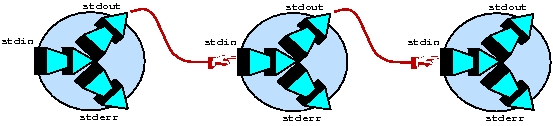
\includegraphics{./_Images/cmds-unix/rapp-filter.jpg}
\caption{\label{fig-cmds-rapp-filter}Rappel sur les filtres}
\end{figure}

\noindent {\bf Propri{\'e}t{\'e}s~:}
\begin{quote}
Par d{\'e}faut, les filtres lisent sur leur entr{\'e}e standard et affichent le
r{\'e}sultat sur leur sortie standard.

Si un fichier est sp{\'e}cifi{\'e} en argument, l'entr{\'e}e standard est redirig{\'e}e
automatiquement sur celui-ci. S'il y en a plusieurs, ils sont mis bout {\`a}
bout et le filtre redirige son entr{\'e}e standard sur le r{\'e}sultat obtenu.
\end{quote}

%%%%%%%%%%%
\subsection{Filtres d{\'e}j{\`a} vus}

La commande \index{cat@\texttt{cat}}"{\tt  cat}" fonctionnecomme un filtre si elle n'a pas
d'arguments. Elle lit sur son entr{\'e}e standard et la r{\'e}affiche sur sa
sortie standard. La figure \ref{fig-cmds-cat} en illustre son fonctionnement.

\begin{figure}[hbtp]
\centering
%\epsfbox{_Images/cmds-unix/cat.eps}
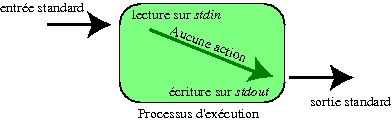
\includegraphics{./_Images/cmds-unix/cat.jpg}
\caption{\label{fig-cmds-cat}Fonctionnement de la commande "{\tt cat}"}
\end{figure}

\begin{remarque}
La commande \index{more@\texttt{more}}"{\tt more}" n'est pas un filtre. Elle lit les
informations sur son entr{\'e}e standard ou bien dans les fichiers pass{\'e}s en
argument, et redirige sur l'{\'e}cran. Elle fait appel aux informations que
le syst{\`e}me connait sur le terminal pour conna{\^\i}tre sa taille, son mode
d'{\'e}mulation, etc{...}
\end{remarque}

%%%%%%%%%%%
\subsection{Filtre {\tt sort}}

\begin{definition}{Syntaxe}
\begin{verbatim}
sort [-nd] [-tcaract{\`e}re] [+num{\'e}ro-champ>] [-num{\'e}ro-champ] 
            [fichier...]
\end{verbatim}
\end{definition}

Le filtre \index{sort@\texttt{sort}}"{\tt sort}" permet de trier les lignes de caract{\`e}res (suite
d'octets d{\'e}limit{\'e}e par le caract{\`e}re \verb=<CR>=) envoy{\'e}es sur l'entr{\'e}e standard
selon un ensemble de crit{\`e}res.

Il est possible de d{\'e}finir un caract{\`e}re s{\'e}parateur de champ afin
d'effectuer des tris sur une zone particuli{\`e}re. Le tri peut se faire~:
\begin{itemize}
	\item soit num{\'e}riquement en sp{\'e}cifiant l'option "{\tt -n}",
	\item soit selon l'ordre {\ASCII} standard (mode par d{\'e}faut),
	\item soit selon l'ordre d{\'e}fini dans un dictionnaire avec l'option
		  "{\tt -d}".
\end{itemize}

Les champs sont d{\'e}limit{\'e}s par d{\'e}faut par une tabulation ou de fa\c{c}on
explicite par le caract{\`e}re sp{\'e}cifi{\'e} avec l'option -t<caract{\`e}re>.

La commande sort lit sur son entr{\'e}e standard, effectue le tri et affiche
le r{\'e}sultat sur sa sortie standard.

Comme la plupart des filtres, la commande "{\tt sort}" accepte des
fichiers en arguments. S'ils sont pr{\'e}cis{\'e}s sur la ligne de commande,
"{\tt sort}" redirige son entr{\'e}e standard sur leur contenu. Il est
{\'e}galement possible de trier sur un champ particulier en utilisant le
symbole "{\tt +}" suivi du num{\'e}ro du champ.

\begin{remarque}
"{\tt sort}" num{\'e}rote les champs {\`a} partir de z{\'e}ro.
\end{remarque}

Si la commande est simple {\`a} utiliser pour effectuer des tris simples,
pour des tris plus complexes, plusieurs tentatives sont bien souvent
n{\'e}cessaires avant de trouver la bonne syntaxe. Ne soyez pas frustr{\'e}s~: la
puissance de la commande pallie cet inconv{\'e}nient. Pour plus de
renseignements, consultez le manuel de r{\'e}f{\'e}rence "{\tt sort(1)}".

\begin{example}
\begin{verbatim}
% sort -nt: +2 /etc/passwd
% ls -R | sort
\end{verbatim}
\end{example}

%%%%%%%%%%%
\subsection{Filtre {\tt grep}}

\begin{definition}{Syntaxe}
\begin{verbatim}
grep [-inv] expression [fichier...]
\end{verbatim}
\end{definition}

Le filtre \index{grep@\texttt{grep}}"{\tt grep}" recherche l'expression pr{\'e}cis{\'e}e sur son entr{\'e}e
standard et l'affiche sur sa sortie standard. Cette expression ob{\'e}it aux
lois des expressions r{\'e}guli{\`e}res {\Unix} (cf. chapitre \ref{reg-exp}).
De fa\c{c}on g{\'e}n{\'e}rale, on sp{\'e}cifie une cha{\^\i}ne de caract{\`e}res.

Les options les plus courantes de la commande "{\tt grep}" sont~:
\begin{itemize}
	\item l'option "{\tt -i}" indique {\`a} "{\tt grep}" qu'il ne faut pas
		  tenir compte des majuscules/minuscules,
	\item l'option "{\tt -v}" indique {\`a} "{\tt grep}" qu'il faut afficher
		  les lignes ne contenant pas l'expression pr{\'e}cis{\'e}e en argument,
	\item l'option "{\tt -n}" permet de voir afficher les num{\'e}ros de
		  lignes courantes.
\end{itemize}

Comme la plupart des filtres, la commande "{\tt grep}" accepte des
fichiers en arguments. S'ils sont pr{\'e}cis{\'e}s sur la ligne de commande,
"{\tt grep}" redirige son entr{\'e}e standard sur leur contenu.

\begin{example}
\begin{verbatim}
% grep user /etc/passwd
% ls -l | grep rwxrwxrwx
\end{verbatim}
\end{example}

%%%%%%%%%%%%
\subsection{Filtre {\tt wc}}

\begin{definition}{Syntaxe}
\begin{verbatim}
wc [-lwc] [fichier{...}]
\end{verbatim}
\end{definition}

Le filtre \index{wc@\texttt{wc}}"{\tt wc}" lit sur son entr{\'e}e standard,  compte le nombre
de lignes (enregistrements s{\'e}par{\'e}s par \verb=<CR>=), le nombre de mots
(enregistrements s{\'e}par{\'e}s par \spacekey ou \tabkey), le nombre de
caract{\`e}res et affiche le r{\'e}sultat sur sa sortie standard.

Les options sont~:\\
\begin{tabular}{l@{\hspace{0.5cm}}l}
	{\tt -l}	&	compte le nombre de lignes,\\
	{\tt -w}	&	compte le nombre de mots,\\
	{\tt -c}	&	compte le nombre de caract{\`e}res.
\end{tabular}

L'ordre des options dans la ligne de commande d{\'e}termine l'ordre de
sortie. Comme la plupart des filtres, la commande "{\tt wc}" accepte
des fichiers en arguments. S'ils sont pr{\'e}cis{\'e}s sur la ligne de commande,
"{\tt wc}" redirige son entr{\'e}e standard sur leur contenu.

\begin{example}
\begin{verbatim}
% wc -l /etc/passwd
% ls -l | wc -l
\end{verbatim}
\end{example}

%%%%%%%%%%%%
\subsection{Filtre {\tt cut}}

\begin{definition}{Syntaxe}
{\tt cut -c{\it liste} [fichier...]}\\
{\tt cut -f{\it liste} [-d{\it caract{\`e}re}] [-s] [fichier...]}
\end{definition}

Le filtre \index{cut@\texttt{cut}}"{\tt cut}" a deux modes de fonctionnement~:

\begin{center}
\begin{tabular}{|p{7cm}|l|}
	\hline
		\multicolumn{1}{|c|}{Mode}		&
		\multicolumn{1}{|c|}{Option}	\\
	\hline \hline
		Extraire des colonnes {\`a} partir de l'entr{\'e}e standard.	&
		option "{\tt -c}"	\\
		Extraire des champs {\`a} partir de l'entr{\'e}e standard.		&
		option "{\tt -f}" \\
	\hline
\end{tabular}
\end{center}

Dans les deux modes, "{\tt liste}" est une s{\'e}quence de num{\'e}ros pour
indiquer {\`a} cut quels sont les champs ou les colonnes {\`a} retenir. Il y a
plusieurs formats possibles pour cette liste~:\\
\begin{tabular}{lp{5cm}}
	"{\tt {\sl A}-{\sl B}}"	&
	champs ou colonnes {\sl A} {\`a} {\sl B} inclus \\
	"{\tt {\sl A}-}"			&
	du champ ou colonne {\sl A} jusqu'{\`a} la fin de la ligne \\
	"{\tt {\sl A},{\sl B}}"	&
	champ ou colonnes {\sl A} et {\sl B} \\
	"{\tt -{\sl B}}"			&
	du d{\'e}but jusqu'au champ ou colonne {\sl B}
\end{tabular}

Toute combinaison des formats pr{\'e}c{\'e}dents est {\'e}galement possible.

\begin{example}
\begin{verbatim}
% cut -f1,4,6-9 /tmp/fictest
\end{verbatim}
extrait du fichier "{\tt /tmp/fictest}" les champs 1, 4 et de 6 {\`a} 9.
\end{example}

Dans le cas d'un d{\'e}coupage par champ, il existe une option particuli{\`e}re,
"{\tt -d}", pour sp{\'e}cifier le caract{\`e}re s{\'e}parateur de champs. Par
d{\'e}faut, ce caract{\`e}re est la tabulation "{\tt TAB}". De m{\^e}me,
l'option "{\tt -s}", lors d'un d{\'e}coupage par champ, indique {\`a} cut
d'{\'e}carter toutes les lignes qui ne contiennent pas le s{\'e}parateur.

\begin{remarque}
La commande "{\tt cut}" commence la num{\'e}rotation des champs {\`a} 1 alors
que "{\tt sort}" commence {\`a} 0. Il y a un moyen facile de s'en rappeler
en notant que sort contient un z{\'e}ro dans son nom (en fait un "{\tt
o}") contrairement {\`a} "{\tt cut}".
\end{remarque}

Comme la plupart des filtres, la commande "{\tt cut}" accepte des
fichiers en arguments. S'ils sont pr{\'e}cis{\'e}s sur la ligne de commande,
"{\tt cut}" redirige son entr{\'e}e standard sur leur contenu.

\begin{example}
\begin{verbatim}
% cut -f3,7 -d: /etc/passwd
% date | cut -c1-3
% ps -ef | cut -c48- | sort
\end{verbatim}
\end{example}
		%% Ok, index

%%%%%%%%%%%%%%%%%%%%%%%%%%%%%%%%%%%%%%%%%%%%%%%%%%%%%%%%%%%%%%%%%%%%%%%%
%                                                                      %
% This program is free software; you can redistribute it and/or modify %
% it under the terms of the GNU General Public License as published by %
% the Free Software Foundation; either version 2 of the License, or    %
% (at your option) any later version.                                  %
%                                                                      %
% This program is distributed in the hope that it will be useful,      %
% but WITHOUT ANY WARRANTY; without even the implied warranty of       %
% MERCHANTABILITY or FITNESS FOR A PARTICULAR PURPOSE.  See the        %
% GNU General Public License for more details.                         %
%                                                                      %
% You should have received a copy of the GNU General Public License    %
% along with this program; if not, write to the Free Software          %
% Foundation, Inc., 51 Franklin St, Fifth Floor, Boston,               %
% MA  02110-1301  USA                                                  %
%                                                                      %
%%%%%%%%%%%%%%%%%%%%%%%%%%%%%%%%%%%%%%%%%%%%%%%%%%%%%%%%%%%%%%%%%%%%%%%%
%
%	$Id$
%

\setcounter{remarque-cnt}{1}
\setcounter{example-cnt}{1}
\chapter{Commandes usuelles de communication r{\'e}seau}
\thispagestyle{fancy}

%%%%%%%%%%%%%%%%%%%%%%%%%%%%%%%%%%%%%%%%%%%%%%%%%%%%
\section{Connexion {\`a} une autre machine -- commande {\tt telnet}}

\begin{definition}{Syntaxe}
\begin{verbatim}
telnet [host [port]]
\end{verbatim}
\end{definition}

La commande \index{telnet@\texttt{telnet}}<<~{\tt telnet}~>> permet de communiquer avec une autre machine en utilisant le protocole {\sl Telnet}. Si <<~{\tt telnet}~>> est invoqu{\'e} sans argument, il passe en mode commande, indiqu{\'e} par l'invite <<~\verb=telnet>=~>>. Dans ce mode, il accepte et ex{\'e}cute des commandes. Si <<~{\tt telnet}~>> est invoqu{\'e} avec des arguments, il ouvre une connexion sur ce qui lui a {\'e}t{\'e} sp{\'e}cifi{\'e}.

Une fois qu'une connexion a {\'e}t{\'e} ouverte, <<~{\tt telnet}~>> passe en mode saisie. Dans ce mode, le texte tap{\'e} au clavier est envoy{\'e} {\`a} la machine cible.

Voici quelques \index{telnet@\texttt{telnet}!commandes internes {\`a}}commandes accessibles au niveau du prompt <<~\verb=telnet>=~>>~:

\begin{description}
	\item[{\tt open [host [port]]}]\mbox{}\\
		Ouvre une connexion sur le n{\oe}ud sp{\'e}cifi{\'e} au port indiqu{\'e}. Si aucun
		port n'est sp{\'e}cifi{\'e}, <<~{\tt telnet}~>> essaie de contacter un serveur
		{\sl Telnet} au port standard de {\sl Telnet}. Le nom de n{\oe}ud peut
		{\^e}tre soit le nom officiel, soit un {\sl alias}, soit une adresse Internet
		en notation d{\'e}cimale.
	\item[{\tt close}]\mbox{}\\
		Ferme une session <<~{\tt telnet}~>>. Si la session a commenc{\'e} en mode
		commande, alors <<~{\tt telnet}~>> repasse en mode commande; autrement,
		{\tt telnet} se termine.
	\item[{\tt ?}]\mbox{}\\
		Fournit de l'aide. Sans argument <<~{\tt ?}~>> affiche le menu d'aide. Si
		une commande est pr{\'e}cis{\'e}e apr{\`e}s <<~{\tt ?}~>>, le message affich{\'e}
		s'applique uniquement {\`a} la commande sp{\'e}cifi{\'e}e.
\end{description}

Pour plus d'informations, consultez {\tt telnet(1)}.

\begin{remarque}
<<~{\tt telnet}~>> est seulement un service interactif. Vous ne pouvez pas ex{\'e}cuter <<~{\tt telnet}~>> en arri{\`e}re-plan ou {\`a} partir d'un programme shell.
\end{remarque}

%%%%%%%%%%%%%%%%%%%%%%%%%%%%%%%%%%%%%%%%%%%%%%%%%%%%
\section{Transfert de fichiers - commande {\tt ftp}}

\begin{definition}{Syntaxe}
\begin{verbatim}
ftp [-g] [-i] [-n] [v] [host]
\end{verbatim}
\end{definition}

\index{ftp@\texttt{ftp}}<<~{\tt ftp}~>> est une famille de commandes pour les op{\'e}rations de manipulation de fichiers ou de r{\'e}pertoires {\`a} travers le r{\'e}seau.

Vous pouvez importer ou exporter des fichiers {\`a} partir d'une machine distante (sous {\Unix} ou non), en utilisant soit le mode de transfert
{\ASCII}, soit le mode de transfert {\sl binaire}.

Vous pouvez~:
\begin{itemize}
	\item mettre {\`a} jour, renommer et supprimer des fichiers,
	\item lister le contenu de r{\'e}pertoires,
	\item changer, cr{\'e}er et supprimer des r{\'e}pertoires,
	\item v{\'e}rifier l'{\'e}tat, changer les options,
	\item demander de l'aide.
\end{itemize}

<<~{\tt ftp}~>> admet quatre \index{ftp@\texttt{ftp}!options}options~:\\
\begin{tabular}{lc@{\hspace{2ex}}p{8cm}}
	{\tt -g}	& : &	inhibition des m{\'e}tacaract{\`e}res.\\
				&   &
		Lorsque cette option n'est pas pr{\'e}cis{\'e}e, par d{\'e}faut, les
		m{\'e}tacaract{\`e}res sont interpr{\'e}t{\'e}s pour l'importation ou l'exportation
		de fichiers. Pour plus de pr{\'e}cisions sur les m{\'e}tacaract{\`e}res,
		reportez vous {\`a} la section \ref{basic-metacars}.
		\\[0.5cm]
	{\tt -i}	& : &	inhibition du mode interactif sur les manipulations de
					fichiers.\\
				&   &
		Le mode interactif est actif par d{\'e}faut.
		\\[0.5cm]
	{\tt -n}	& : &	d{\'e}sactivation de la connexion automatique.\\
				&   &
		 La connexion automatique est autoris{\'e}e.
		\\[0.5cm]
	{\tt -v}	& : &	mode {\sl verbose}.\\
				&   &
		En l'absence de cette option, <<~{\tt ftp}~>> utilise le mode {\sl verbose}
		uniquement si la sortie standard est associ{\'e}e {\`a} un terminal.
		\\[0.5cm]
\end{tabular}

Quelques-unes des commandes de <<~{\tt ftp}~>> sont expliqu{\'e}es ci-dessous. Dans les explications, <<~{\tt server-host}~>> d{\'e}signe la machine sur laquelle on se connecte avec <<~{\tt ftp}~>>. <<~{\tt local-host}~>> d{\'e}signe la machine sur laquelle la commande <<~{\tt ftp}~>> a {\'e}t{\'e} lanc{\'e}e. La figure
\ref{fig-cmdnet-ftpdesc} illustre les terminologies utilis{\'e}es.

\begin{figure}[hbtp]
\centering
%\epsfbox{_Images/cmds-net/ftpdesc.eps}
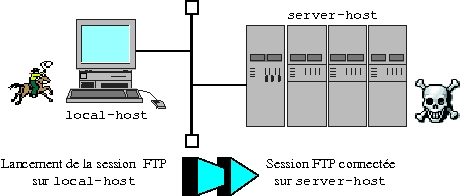
\includegraphics{cmds-net/ftpdesc}
\caption{\label{fig-cmdnet-ftpdesc}Terminologie pour la description de
		<<~{\tt ftp}~>>.}
\end{figure}

{\bf Apercu des \index{ftp@\texttt{ftp}!commandes internes {\`a}}commandes {\tt ftp}~:}\\
\begin{description}
	\item[{\tt open server-host [port-number]}]\mbox{}\\
	Etablit une connexion avec <<~{\tt server-host}~>> en utilisant un num{\'e}ro de port
	si sp{\'e}cifi{\'e}. Si aucun port n'est pr{\'e}cis{\'e}, <<~{\tt ftp}~>> essaie de
	contacter un serveur avec le num{\'e}ro de port standard.

	\item[{\tt user user\_name [password] [account]}]\mbox{}\\
	Connexion sous l'identit{\'e} <<~{\tt user\_name}~>> sur <<~{\tt
	server-host}~>> ouverte avec la commande <<~{\tt open}~>>. La figure
	\ref{fig-cmdnet-ftpconn} illustre l'{\'e}tablissement d'une connexion.
	\begin{figure}[hbtp]
	\centering
%	\epsfbox{_Images/cmds-net/ftpconn.eps}
	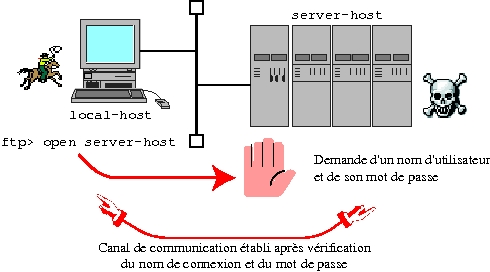
\includegraphics{cmds-net/ftpconn}
	\caption{\label{fig-cmdnet-ftpconn}Etablissement d'une connexion {\tt ftp}}
	\end{figure}

	\item[{\tt glob}]\mbox{}\\
	Autorise l'usage des m{\'e}tacaract{\`e}res. Si cette option est activ{\'e}e,
	<<~{\tt ftp}~>> envoie les m{\'e}tacaract{\`e}res {\`a} <<~{\tt server-host}~>> pour qu'il
	puisse les interpr{\'e}ter au niveau des noms de fichiers et des
	r{\'e}pertoires existants. La substitution des m{\'e}tacaract{\`e}res est
	toujours faite avec la commande <<~{\tt ls}~>>. Pour plus de pr{\'e}cisions
	sur les m{\'e}tacaract{\`e}res, preportez-vous {\`a} la section \ref{basic-metacars}.

	\item[{\tt binary}]\mbox{}\\
	Positionne l'option binaire pour le type de transfert de fichiers.

	\item[{\tt ls [remote\_dir [local\_file]]}]\mbox{}\\
	Affiche les noms des fichiers du site distant <<~{\tt remote\_dir}~>>
	{\`a} l'{\'e}cran, ou {\'e}ventuellement la redirige dans un fichier local
	<<~{\tt local\_file}~>>. Si <<~{\tt remote\_dir}~>> et <<~{\tt
	local\_file}~>> ne sont pas pr{\'e}cis{\'e}s,alors le r{\'e}pertoire de travail
	distant est affich{\'e} sur la sortie standard.


	\item[{\tt put local\_file [remote\_file]}]\mbox{}\\
	Copie un fichier local <<~{\tt local\_file}~>> vers le site distant
	sous le nom <<~{\tt remote\_file}~>>. Si <<~{\tt remote\_file}~>> n'est
	pas sp{\'e}cifi{\'e}, <<~{\tt ftp}~>> copie le fichier sous le m{\^e}me nom. La figure
	\ref{fig-cmdnet-ftpexch} illustre l'envoi et la r{\'e}ception de fichiers
	entre un serveur et un client <<~{\tt ftp}~>>.


	\item[{\tt mput local\_file local\_file ...}]\mbox{}\\
	Copie plusieurs fichiers du site local vers le site distant. Les
	fichiers de destination ont les m{\^e}mes noms que les fichiers locaux
	d'origine. Si l'option <<~{\tt glob}~>> est activ{\'e}e, les
	m{\'e}tacaract{\`e}res sont interpr{\'e}t{\'e}s. La figure \ref{fig-cmdnet-ftpexch}
	illustre l'envoi et la r{\'e}ception de fichiers entre un serveur et un
	client <<~{\tt ftp}~>>.


	\item[{\tt get remote\_file [local\_file]}]\mbox{}\\
	Copie un fichier distant <<~{\tt remote\_file}~>> sur le syst{\`e}me local
	sous le nom <<~{\tt local\_file}~>>. Si <<~{\tt local\_file}~>> n'est
	pas pr{\'e}cis{\'e}, <<~{\tt ftp}~>> copie le fichier avec le m{\^e}me nom. La figure
	\ref{fig-cmdnet-ftpexch} illustre l'envoi et la r{\'e}ception de fichiers
	entre un serveur et un client <<~{\tt ftp}~>>.


	\item[{\tt mget remote\_file remote\_file ...}]\mbox{}\\
	Copie plusieurs fichiers distants vers le syst{\`e}me local. Si l'option
	<<~{\tt glob}~>> est activ{\'e}e, les m{\'e}tacaract{\`e}res sont interpr{\'e}t{\'e}s. La figure
	\ref{fig-cmdnet-ftpexch} illustre l'envoi et la r{\'e}ception de fichiers
	entre un serveur et un client <<~{\tt ftp}~>>.

	\begin{figure}[hbtp]
	\centering
%	\epsfbox{_Images/cmds-net/ftpexch.eps}
	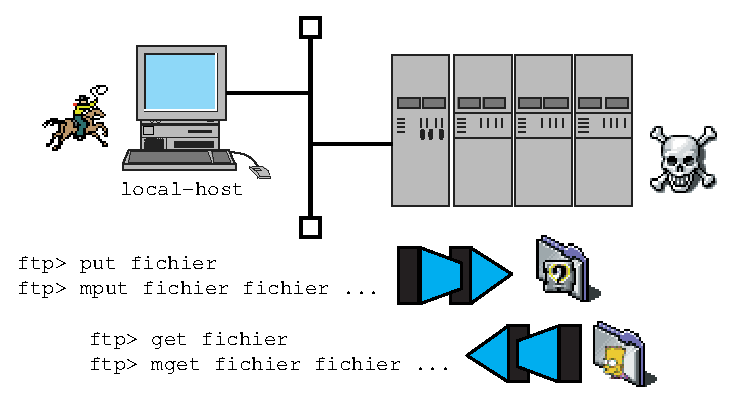
\includegraphics{cmds-net/ftpexch}
	\caption{\label{fig-cmdnet-ftpexch}Envoi/R{\'e}ception de fichier(s) de
	<<~{\tt server-host}~>> vers <<~{\tt local-host}~>> avec <<~{\tt ftp}~>>.}
	\end{figure}

	\item[{\tt close}]\mbox{}\\
	Ferme la connexion avec <<~{\tt server-host}~>>. La commande <<~{\tt
	close}~>> ne permet pas de sortir de <<~{\tt ftp}~>> si la connexion a {\'e}t{\'e}
	{\'e}tablie avec une commande <<~{\tt open}~>>.

	\item[{\sl {\tt quit} ou {\tt bye}}]\mbox{}\\
	Les commandes <<~{\tt quit}~>> et <<~{\tt bye}~>> ont le m{\^e}me effet.
	Elles ferment la connexion avec <<~{\tt server-host}~>> si une
	connexion {\'e}tait ouverte et sort de <<~{\tt ftp}~>>.
\end{description}

\begin{example}
{\bf Utilisation de <<~{\tt ftp}~>> dans un programme shell}
\begin{quote}
Vous pouvez utiliser <<~{\tt ftp}~>> dans un programme shell en respectant
certaines r{\`e}gles. Voici un exemple d'utilisation de <<~{\tt ftp}~>> dans un
programme Bourne Shell.

\begin{verbatim}
(
    for host in willow arthur merlin
    do
        echo "
            open $host
            user lancelot dulac
            binary
            mput excalibur*
            close
        "
    done
) | ftp -i -n
\end{verbatim}

Ce programme shell repr{\'e}sente un risque au niveau de la s{\'e}curit{\'e} (mot de passe en clair dans une proc{\'e}dure). Ce type de programme est {\`a} utiliser avec parcimonie. Pour plus de renseignements, consultez <<~{\tt ftp(1)}~>>.
\end{quote}
\end{example}

%%%%%%%%%%%%%%%%%%%%%%%%%%%%%%%%%%%%%%%%%%%%%%%%%%%%%%%
\section{Connexion automatique -- commande {\tt rlogin}}

\begin{definition}{Syntaxe}
{\tt rlogin remote\_host [-e{\it c}] [-l {\it username}]}
\end{definition}

La commande \index{rlogin@\texttt{rlogin}}<<~{\tt rlogin}~>> connecte votre terminal du site local sur un n{\oe}ud distant. <<~{\tt rlogin}~>> agit comme un terminal virtuel sur le syst{\`e}me distant. Le nom de machine distante peut {\^e}tre le nom officiel ou bien un {\sl alias}\footnote{Nom secondaire au niveau de la configuration r{\'e}seau.}. Il est possible aussi d'utiliser l'adresse Internet. Le type de terminal (indiqu{\'e} par la variable <<~{\tt TERM}~>>) est propag{\'e} {\`a} travers le r{\'e}seau et est utilis{\'e} pour initialiser la variable <<~{\tt TERM}~>> sur le site distant. Pour plus de renseignements sur les variables d'environnement du shell, reportez vous {\`a} la section \ref{basicn-codevar}.

Une fois connect{\'e} au site distant, vous pouvez ex{\'e}cuter des commandes sur le site local en utilisant le caract{\`e}re d'{\'e}chapement (par d{\'e}faut <<~{\verb=~=}~>>). Une ligne commen\c{c}ant par <<~\verb=~!=~>> cr{\'e}e un shell et vous permet d'ex{\'e}cuter temporairement des commandes sur le site local. Une ligne commen\c{c}ant par <<~\verb=~=~>> vous d{\'e}connecte du site distant. Plus simplement, pour revenir {\`a} votre session de d{\'e}part, il suffit de taper la commande <<~{\tt exit}~>> sur le site distant.

\begin{example}
\verb=dragon % rlogin king -l arthur=\\
\verb=Password:=\\
\verb=Welcome on IRIX 4.5 4D/480 to node king=\\
\verb=king% ~!=\\
\verb=dragon %=\hfill \hfill (vous {\^e}tes de retour sur votre terminal local)\\
$\cdots$\\
\verb=dragon % exit=\hfill \hfill(vous retournez {\`a} la station distante)\\
\verb=king%=
\end{example}

Les options de rlogin sont d{\'e}crites ci-dessous~:\\[0.5ex]
\begin{tabular}{lp{8cm}}
	{\tt -e{\it c}}		&
	Positionne le caract{\`e}re d'{\'e}chappement {\`a} <<~{\tt c}~>>. Il n'y a pas d'espace
	entre le caract{\`e}re <<~{\tt e}~>> et le caract{\`e}re d'{\'e}chappement.\\
	{\tt -l {\it username}}	&
	Met le nom de connexion de l'utilisateur sur le site distant {\`a} <<~{\tt
	username}~>>. Par d{\'e}faut, le nom de connexion de l'utilisateur sur le
	site local est utilis{\'e} pour se connecter au site distant.
\end{tabular}

Pour plus de renseigements, consultez <<~{\tt rlogin(1)}~>>.

%%%%%%%%%%%%%%%%%%%%%%%%%%%%%%%%%%%%%%%%%%%%%%%%%%%%%%%
\section{Transfert de fichiers automatique -- commande {\tt rcp}}

\begin{definition}{Syntaxe}
{\tt rcp {\it source} {\it destination}}

avec {\it source} et {\it destination} de la forme {\tt [[{\it user}@]{\it host}:]{\it pathname}}
\end{definition}

La commande \index{rcp@\texttt{rcp}}<<~{\tt rcp}~>> est similaire {\`a} la commane <<~{\tt cp}~>> d'{\Unix}. Comme <<~{\tt cp}~>>, <<~{\tt rcp}~>> aura un comportement diff{\'e}rent selon le nombre d'arguments~:

\begin{itemize}
	\item	si elle ne poss{\`e}de que deux arguments, elle copie le fichier source
			sous le nouveau nom,
	\item	si elle poss{\`e}de plusieurs arguments, la destination est
			obligatoirement un r{\'e}pertoire. Dans ce cas, elle copie les fichiers
			sources dans le r{\'e}pertoire sp{\'e}cifi{\'e}.
\end{itemize}

<<~{\tt rcp}~>> ne demande pas de mot de passe si une {\'e}quivalence syst{\`e}me ou utilisateur a {\'e}t{\'e} configur{\'e}e.

Dans le cas contraire, elle ne fonctionne pas (message <<~{\tt Permission denied}~>>). <<~{\tt rcp}~>> autorise des transferts mettant en jeu plusieurs machines. Par exemple, si vous {\^e}tes connect{\'e} sur une machine, vous pouvez transf{\'e}rer des fichiers entre deux n{\oe}uds du r{\'e}seau totalement diff{\'e}rents.

La source et la destination se pr{\'e}sentent sous la forme
{\tt [[{\it user}@]{\it host}:]{\it pathname}} avec~:\\
\begin{center}
\begin{tabular}{lp{8cm}}
	{\tt host}		&
	Sp{\'e}cifie le syst{\`e}me sur lequel se trouve le fichier. Si <<~{\tt
	host}~>> n'est pas pr{\'e}cis{\'e}, le syst{\`e}me local est utilis{\'e} par d{\'e}faut.\\
	{\tt user}		&
	Sp{\'e}cifie l'utilisateur sur <<~{\tt host}~>>. Si <<~{\tt user}~>> n'est
	pas pr{\'e}cis{\'e}, l'utilisateur sur le site distant est le m{\^e}me que sur
	le site local (les noms des utilisateurs doivent correspondre d'un
	syst{\`e}me {\`a} l'autre).\\
	{\tt pathname}	&
	Donne le chemin du fichier {\`a} copier. Il peut {\^e}tre relatif ou absolu.
	Un chemin relatif est interpr{\'e}t{\'e} de mani{\`e}re relative par rapport au
	r{\'e}pertoire de connexion sur le site distant ou par rapport au
	r{\'e}pertoire courant sur le site local.
\end{tabular}
\end{center}

Il est possible d'utiliser les m{\'e}tacaract{\`e}res pour r{\'e}f{\'e}rencer des fichiers. N'oubliez pas que le shell local interpr{\`e}te n'importe quel m{\'e}tacaract{\`e}re avant d'appeler <<~{\tt rcp}~>>. Pour emp{\^e}cher une substitution locale des m{\'e}tacaract{\`e}res devant {\^e}tre trait{\'e}s par le site distant, mettez les entre simples quotes (cf. section \ref{basic-quotes}).

\begin{example}
\label{exp-cmdnet-exrcp}
On supposera que toutes les {\'e}quivalences utilisateur et syst{\`e}me ont {\'e}t{\'e} configur{\'e}es correctement.

Le processus de cet exemple est d{\'e}crit au tableau \ref{tab-cmdnet-exrcp} et {\`a} la figure \ref{fig-cmdnet-exrcp}.
\end{example}

Dans la configuration d{\'e}crite dans la figure \ref{fig-cmdnet-exrcp},\\
\begin{longtable}{|c|p{8cm}|}
	\hline
	\multicolumn{2}{|r|}{Suite de la page pr{\'e}c{\'e}dente.} \\
	\hline
	\multicolumn{1}{|c|}{Exemple}		&
	\multicolumn{1}{|c|}{Description}	\\
	\hline
\endhead
	\hline
	\multicolumn{1}{|c|}{Exemple}		&
	\multicolumn{1}{|c|}{Description}	\\
	\hline
\endfirsthead
	\hline
		\multicolumn{2}{|r|}{Suite page suivante $\cdots$} \\
	\hline
\endfoot
	\hline
\endlastfoot
	\hline
 	\raisebox{-0.5cm}{
%\epsfbox{_Images/cmds-net/exrcp-cl1.eps}

\includegraphics{cmds-net/exrcp-cl1}
}	&
	L'utilisateur {\tt willow} sur la machine {\tt dragon} copie le
	fichier {\tt excalibur.c} de l'utilisateur {\tt arthur} sur la
	machine {\tt king} dans son r{\'e}pertoire courant.
	\\
	\hline
  	\raisebox{-0.5cm}{
%\epsfbox{_Images/cmds-net/exrcp-cl2.eps}
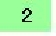
\includegraphics{cmds-net/exrcp-cl2}
}	&
	L'utilisateur {\tt willow} sur la machine {\tt dragon} copie le
	fichier local {\tt donjon.c} sur la machine {\tt dragon} vers le
	r{\'e}pertoire de connexion de l'utilisateur {\tt willow} sur la machine
	{\tt dulac}.
	\\
	\hline
 	\raisebox{-0.5cm}{
%\epsfbox{_Images/cmds-net/exrcp-cl3.eps}
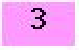
\includegraphics{cmds-net/exrcp-cl3}
}	&
	L'utilisateur {\tt willow} sur la machine {\tt dragon} copie tous les
	fichiers <<~{\tt .c}~>> de l'utilisateur {\tt arthur} sur la machine
	{\tt king} vers son r{\'e}pertoire courant.
	\\
	\hline
 	\raisebox{-0.5cm}{
%\epsfbox{_Images/cmds-net/exrcp-cl4.eps}
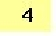
\includegraphics{cmds-net/exrcp-cl4}
}	&
	L'utilisateur {\tt willow} sur la machine {\tt dragon} copie le
	fichier {\tt excalibur.c} de l'utilisateur {\tt arthur} sur la
	machine {\tt king} vers le r{\'e}pertoire de connexion de l'utilisateur
	{\tt lancelot} sur la machine {\tt dulac}.
	\\
	\hline
\caption*{\label{tab-cmdnet-exrcp}Description des op{\'e}rations effectu{\'e}es.}
\end{longtable}

On obtient l'exemple illustr{\'e} dans la figure \ref{fig-cmdnet-exrcp}.

\begin{figure}
\centering
%\epsfbox{_Images/cmds-net/exrcp.eps}
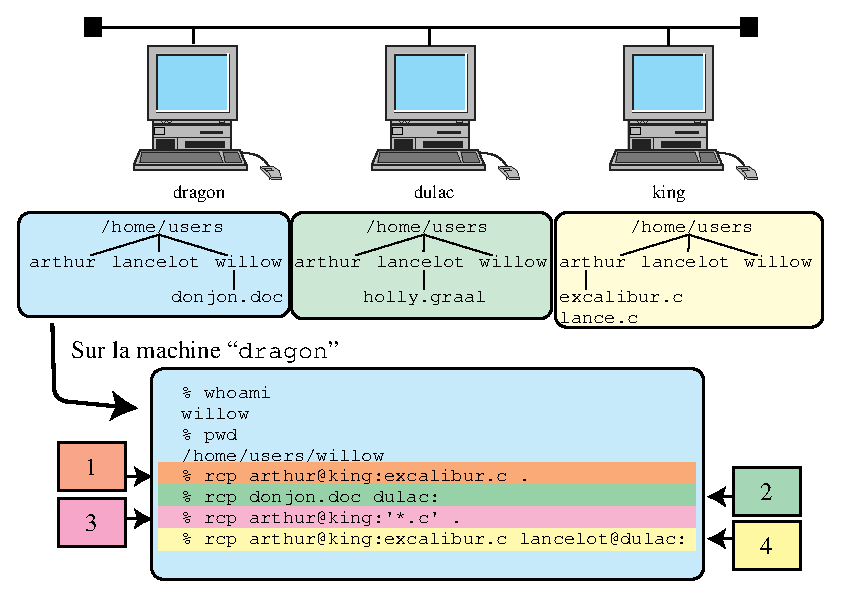
\includegraphics{cmds-net/exrcp}
\caption{\label{fig-cmdnet-exrcp}Exemple d'utilisation de la commande <<~{\tt rcp}~>>.}
\end{figure}


%%%%%%%%%%%%%%%%%%%%%%%%%%%%%%%%%%%%%%%%%%%%%%%%%%%%%%%
\section{Ex{\'e}cution d'une commande {\`a} distance - commande {\tt rsh} (ou {\tt remsh})}

\begin{definition}{Syntaxe}
{\tt rsh [-l {\it username}] [-n] {\it commande}}\\
{\tt remsh [-l {\it username}] [-n] {\it commande}}
\end{definition}

Les commandes \index{rsh@\texttt{rsh}}<<~\texttt{rsh}~>> et \index{remsh@\texttt{remsh}}<<~\texttt{remsh}~>> sont {\'e}quivalentes.
Sur certains syt{\`e}mes il n'exite que la commande <<~\texttt{rsh}~>>\footnote{\textsl{SunOS} et  \textsl{Solaris} sur les syst{\`e}mes de Sun Microsystems, \textsl{Irix} sur les machines de Silicon Graphics, \textsl{Digital {\Unix}} sur les machines de Compacq - ex Digital Equipment Corp.}, sur d'autres que seule la commande <<~{\tt remsh}~>> sera disponible\footnote{\textsl{UTekV} sur les anciens syst{\`e}mes {\Unix} de Tektronix, \textsf{HP--UX} sur les syst{\`e}mes de Hewlett-Packard}), sur d'autres les deux cohabiteront\footnote{AIX, l'{\Unix} d'IBM}. Dans toute la suite de ce paragraphe, seulement <<~\texttt{rsh}~>> sera cit{\'e}.

La commande <<~{\tt rsh}~>> ex{\'e}cute une commande non interactive sur un syst{\`e}me distant. Le nom du compte est le m{\^e}me que le nom du compte local {\`a} moins que vous ne sp{\'e}cifiez l'option <<~{\tt -l}~>>.

Comme <<~{\tt rcp}~>>, <<~{\tt rsh}~>> ne demande pas de mot de passe si une {\'e}quivalence syst{\`e}me ou utilisateur a {\'e}t{\'e} configur{\'e}e. Dans le cas contraire, elle ne fonctionne pas (message <<~{\tt Permission denied}~>>). La commande <<~{\tt rsh}~>> transmet les signaux <<~{\tt INTERRUPT}~>>, <<~{\tt QUIT}~>> et <<~{\tt HUP}~>> {\`a} la commande distante.

Pour plus de pr{\'e}cisions, reportez vous {\`a} <<~{\tt signal(2)}~>> et au chapitre \ref{multitask}.

Vous pouvez utiliser les m{\'e}tacaract{\`e}res avec <<~{\tt rsh}~>>. Si vous voulez qu'ils soient interpr{\'e}t{\'e}s sur le site distant, assurez-vous qu'ils sont bien entre simples quotes (cf. sections \ref{basic-metacars} et \ref{basic-quotes}).

\begin{remarque}
<<~{\tt rsh}~>> ne peut pas ex{\'e}cuter des commandes en mode interactif comme
<<~{\tt vi}~>>, <<~{\tt emacs}~>>, etc.
\end{remarque}

%%%%%%%%%%%%%%%%%%%%%%%%%%%%%%%%%%%%%%%%%%%%%%%%%%%%
\section{Connexion chiffr{\'e}e {\`a} une autre machine -- commande {\tt ssh}}
Les commandes pr{\'e}c{\'e}dentes ont non seulement des limitations (<<~{\tt rsh}~>> ne permet, par exemple, d'ex{\'e}cuter des commandes interactives) mais posent aussi des probl{\`e}mes de s{\'e}curit{\'e}. D{\'e}sormais, le protocole \index{ssh@\texttt{ssh}}<<~\texttt{ssh}~>> (\href{http://fr.wikipedia.org/wiki/Secure_shell/}{Secure SHell}), et la commande qui lui est associ{\'e}, est donc aujourd'hui le plus souvent utilis{\'e}, {\`a} la place de rlogin ou rsh .
Caract{\'e}ristique important, le protocole impose, au d{\'e}but de la communication, l'{\'e}change de cl{\'e} de cryptage, permettant au reste de la dialogue de s'effectuer de mani{\`e}re chiffr{\'e}.
L'implementation de <<~{\tt ssh}~>> la plus courament utilis{\'e} est celle du projet libre \href{http://www.openssh.org/fr/index.html}{OpenSSH}.
\begin{definition}{Syntaxe}
\begin{verbatim}
ssh [user]@[host:[port]]
\end{verbatim}
\end{definition}
Un rapide exemple de connexion sur une machine distante {\`a} l'aide de ssh:
\begin{verbatim}
ssh -l arthur percival -p 22
\end{verbatim}

La syntaxe suivante, plus explicite, est aussi possible:
\begin{verbatim}
ssh arthur@percival:22 
\end{verbatim}


\begin{remarque}
Le client <<~{ssh}~>> est un outil extremement puissant, qui permet, entre autres l'{\'e}tablissement de tunnel chiffr{\'e}, {\`a} travers plusieurs machines. N'h{\'e}sitez pas {\`a} en explorer les capacit{\'e}s. L'article \href{http://www.unixgarden.com/index.php/administration-systeme/principes-et-utilisation-de-ssh}{principe et utilisation de SSH} vous permettra d'aller plus loin.
\end{remarque}
% 
\begin{remarque}
Le client <<~{ssh}~>> peut tre utilis{\'e} comme un filtre, mais de mani{\`e}re assez particuli{\`e}re. Un rapide exemple pour illuster ce point:
\begin{verbatim}
cat mon\_fichier | ssh percival ``cat > mon\_fichier\_distant'' 
\end{verbatim}

La commande local cat va transf{\'e}rer vers ssh le contenu du mon\_fichier, ce dernier va le mettre {\`a} disposition sur le flux d'entr{\'e} du serveur distant (percival). Sur ce dernier, la commande cat va permettre de rediriger le flux vers mon\_fichier\_distant. 
\end{remarque}

\section{Transfert chiffr{\'e}e de fichier -- commande scp}
La commande  \index{scp@\texttt{scp}}<<~\texttt{scp}~>> permet d'utiliser le protocole ssh pour transf{\'e}rer des fichiers, mais dans un flux chiffr{\'e}. 

Attention, il est important (et {\'e}vident) de retenir que tout {\'e}change de fichier par ssh sera plus long et plus consommateur de resources du syst{\`e}me qu'un simple transfert en clair.
\begin{definition}{Syntaxe}
\begin{verbatim}
scp [user]@[host:[port]]file [user]@[host:[port]]fichier 
\end{verbatim}
\end{definition}



\subsection{Comparaisons \texttt{telnet}/\texttt{rlogin}/\texttt{ssh} et \texttt{ftp}/\texttt{rcp}/\texttt{scp}}

\index{telnet@\texttt{telnet}!comparaison avec \texttt{rlogin} et \texttt{ssh}}
\index{ssh@\texttt{ssh}!comparaison avec \texttt{rlogin} et \texttt{telnet}}
\index{rlogin@\texttt{rlogin}!comparaison avec \texttt{telnet}}
\begin{longtable}{|p{6.5cm}|p{2cm}|p{2cm}|p{2cm}|}
	\hline
		\multicolumn{4}{|r|}{Suite de la page pr{\'e}c{\'e}dente.} \\
	\hline
		\multicolumn{1}{|c|}{Fonctionnalit{\'e}}	&
		\multicolumn{1}{|c|}{{\tt telnet}}	&
		\multicolumn{1}{|c|}{rlogin}	&
		\multicolumn{1}{|c|}{ssh}	\\
	\hline
\endhead
	\hline
		\multicolumn{1}{|c|}{Fonctionnalit{\'e}}	&
		\multicolumn{1}{|c|}{{\tt telnet}}	&
		\multicolumn{1}{|c|}{rlogin}	&
		\multicolumn{1}{|c|}{ssh}	\\
	\hline \hline
\endfirsthead
	\hline
		\multicolumn{4}{|r|}{Suite page suivante $\cdots$} \\
	\hline
\endfoot
	\hline
\endlastfoot
	\hline
		Ensemble de commandes.		&
		Oui				&
		Non				&
		Oui				\\
	\hline
		Peut se connecter {\`a} des syst{\`e}mes non {\Unix}.	&
		Oui								&
		Non\footnote{D{\'e}pend de l'implantation sur le syst{\`e}me non-{\Unix}.}	&
		Oui\footnote{Si le syst{\`e} h{\^o}te dispose d'un serveur SSH, ce qui est g{\'e}n{\'e}ralement le cas. Pour indication, OpenSSH fonctionne sur Windows et OpenVMS.} \\
	\hline
		Peut {\^e}tre configur{\'e} en connexion automatique.	&
		Non								&
		Oui (fichiers {\tt /etc/hosts.equiv} et {\tt \~/.rhosts})	&
		Oui(Utilisation de cl{\'e} priv{\'e}e)	\\
	\hline
		Peut utiliser l'adresse IP pour la connexion.	&
		Oui								&
		Oui								&
		Non								\\
	\hline
		Sortie autoris{\'e}e.				&
		Oui (vers <<~{\tt telnet}~>> en mode commande)	&
		Oui (vers le terminal local)			&
		Oui						\\
	\hline
		Nombre de modes.				&
		2 (commande et connect{\'e})			&
		1 (connect{\'e} seulement)			&
		1 (connection partageable\footnote{Avec l'option -o ControlMaster})	\\
	\hline
		Peut {\^e}tre lac{\'e} depuis un programme Shell.	&
		Non													&
		Non													&
		Oui													\\
	\hline
\caption{Comparaisons {\tt telnet}/{\tt rlogin}/{\tt ssh}} \\
\end{longtable}

\begin{remarque}
Notez que <<~{\tt telnet}~>> et <<~{\tt rlogin}~>> peuvent {\^e}tre appel{\'e}s
depuis un programme Shell, mais vous ne pouvez pas leur transmettre des
informations au clavier (comme vous pouvez le faire avec <<~{\tt ftp}~>>).
\end{remarque}

\index{ftp@\texttt{ftp}!comparaison avec \texttt{rcp} et \texttt{scp}}
\index{rcp@\texttt{rcp}!comparaison avec \texttt{ftp} et \texttt{scp}}
\index{scp@\texttt{scp}!comparaison avec \texttt{ftp} et \texttt{rcp}}
\begin{longtable}{|p{6.5cm}|p{2cm}|p{2cm}|p{2cm}|}
	\hline
		\multicolumn{4}{|r|}{Suite de la page pr{\'e}c{\'e}dente.} \\
	\hline
		\multicolumn{1}{|c|}{Fonctionnalit{\'e}}	&
		\multicolumn{1}{|c|}{{\tt ftp}}			&
		\multicolumn{1}{|c|}{{\tt rcp}}			&
		\multicolumn{1}{|c|}{{\tt scp}}		\\
	\hline
\endhead
	\hline
		\multicolumn{1}{|c|}{Fonctionnalit{\'e}}	&
		\multicolumn{1}{|c|}{{\tt ftp}}			&
		\multicolumn{1}{|c|}{{\tt rcp}}			&
		\multicolumn{1}{|c|}{{\tt scp}}		\\
	\hline \hline
\endfirsthead
	\hline
		\multicolumn{4}{|r|}{Suite page suivante $\cdots$} \\
	\hline
\endfoot
	\hline
\endlastfoot
	\hline
		Ensemble de commandes	&
		Oui						&
		Non						&
		Oui						\\
	\hline
		Peut transf{\'e}rer des fichiers sur un syst{\`e}me non {\Unix}	&
		Oui						&
		Non\footnote{Sauf impl{\'e}mentation d'un serveur supportant
		ce type de connexion.}				&
		Non\footnote{Sauf impl{\'e}mentation d'un serveur supportant
		ce type de connexion.}				\\
	\hline
		Peut {\^e}tre ex{\'e}cut{\'e} dans un programme Shell	&
		Oui						&
		Oui						&
		Oui						\\
	\hline
		Peut mettre en jeu 3 n{\oe}uds	&
		Non		&
		Oui		&
		Oui		\\
	\hline
		Autorise les m{\'e}tacaract{\`e}res	&
		Oui (commande <<~{\tt glob}~>>)		&
		Oui					&
		Non					\\
	\hline
		Peut faire une copie r{\'e}cursive	&
		Non					&
		Oui (option <<~{\tt -r}~>>)		&
		Oui (option <<~{\tt -r}~>>)		\\
	\hline
		Peut configurer une {\'e}quivalence utilisateur				&
		Oui (fichier <<~{\tt \~/.netrc}~>>)					&
		Oui (fichiers <<~{\tt /etc/hosts.equiv}~>>, <<~{\tt \~/.rhosts}~>>)	&
		Oui (cl{\'e} priv{\'e}e)	\\
	\hline
		Equivalence utilisateur requise		&
		Non					&
		Oui					&
		Oui					\\
	\hline
		Peut utiliser une adresse IP pour la connexion	&
		Oui		&
		Oui		&
		Non		\\
	\hline
\caption{Comparaisons {\tt ftp}/{\tt rlogin}/{\tt scp}} \\
\end{longtable}
	%% Ok, index

%%%%%%%%%%%%%%%%%%%%%%%%%%%%%%%%%%%%%%%%%%%%%%%%%%%%%%%%%%%%%%%%%%%%%%%%
% Partie 2
%%%%%%%%%%%%%%%%%%%%%%%%%%%%%%%%%%%%%%%%%%%%%%%%%%%%%%%%%%%%%%%%%%%%%%%%
\mypart{Introduction au shell}

%%%%%%%%%%%%%%%%%%%%%%%%%%%%%%%%%%%%%%%%%%%%%%%%%%%%%%%%%%%%%%%%%%%%%%%%
%                                                                      %
% This program is free software; you can redistribute it and/or modify %
% it under the terms of the GNU General Public License as published by %
% the Free Software Foundation; either version 2 of the License, or    %
% (at your option) any later version.                                  %
%                                                                      %
% This program is distributed in the hope that it will be useful,      %
% but WITHOUT ANY WARRANTY; without even the implied warranty of       %
% MERCHANTABILITY or FITNESS FOR A PARTICULAR PURPOSE.  See the        %
% GNU General Public License for more details.                         %
%                                                                      %
% You should have received a copy of the GNU General Public License    %
% along with this program; if not, write to the Free Software          %
% Foundation, Inc., 51 Franklin St, Fifth Floor, Boston,               %
% MA  02110-1301  USA                                                  %
%                                                                      %
%%%%%%%%%%%%%%%%%%%%%%%%%%%%%%%%%%%%%%%%%%%%%%%%%%%%%%%%%%%%%%%%%%%%%%%%
%
%	$Id$
%

\setcounter{remarque-cnt}{1}
\setcounter{example-cnt}{1}
\chapter{Notions {\'e}l{\'e}mentaires du Bourne Shell}

%%%%%%%%%%%%%%%%%%%%%%%%%%%%%%%%%%%%%%%%%%%%%%%%%%%%%%%%%%%%%%%%%%%%%
\section{Introduction}

Le \index{shell}shell est un interpr{\'e}teur de commandes qui~:
\begin{itemize}
	\item initialise l'environnement,
	\item g{\'e}n{\`e}re le prompt.
\end{itemize}

Quand une commande est valid{\'e}e, le shell
\begin{enumerate}
	\item  effectue les substitutions de variables,
	\item interpr{\`e}te les m{\'e}tacaract{\`e}res,
	\item g{\`e}re les redirections et les pipes,
	\item effectue les substitutions de commandes,
	\item ex{\'e}cute la commande.
\end{enumerate}
C'est le \index{shell!m{\'e}canisme
d'{\'e}valuation}\textbf{m{\'e}canisme d'{\'e}valuation du shell}. Ces 
{\'e}tapes sont {\`a} garder en {\'e}moire pour toute commande saisie au
clavier ou bien enregistr{\'e}e dans un script.{\Large Ce n'est pas ce
qui est saisi qui sera ex{\'e}cut{\'e} \textbf{mais le r{\'e}sultat de
l'{\'e}valuation de l'expression}.}

Il existe plusieurs shells sous {\Unix}~:
\begin{itemize}
	\item	le Bourne Shell (not{\'e} \index{shell!sh@\texttt{sh}}"\texttt{sh}") anc{\^e}tre de tous les shells,
			utilis{\'e}s seulement pour l'{\'e}criture de proc{\'e}dures. Il n'offre aucune
			facilit{\'e} pour l'emploi en mode interactif (pas d'historique de 
			commandes, pas de rappels avec les fl{\`e}ches, etc.).
	\item	le C Shell (not{\'e} \index{shell!csh@\texttt{csh}}"\texttt{csh}") plut{\^o}t concu pour une interface avec
			les utilisateurs. Il permet le rappel des commandes avec les fl{\`e}ches,
			de g{\'e}rer une historique des commandes, etc. Sa syntaxe 
			se rapproche de celle du langage C m{\^e}me si le "\textsl{C}"
			veut dire "\textsl{California}"\footnote{Ce shell a {\'e}t{\'e} d{\'e}velopp{\'e} {\`a}
			l'universit{\'e} "\textsl{UCB}", University of California -- Berkeley.}.
	\item	le Korn Shell (not{\'e} \index{shell!ksh@\texttt{ksh}}"\texttt{ksh}") est une extension du Bourne Shell
			avec une partie des possibilit{\'e}s du C Shell.
	\item	le Bourne Again Shell (not{\'e} \index{shell!bash@\texttt{bash}}"\texttt{bash}") est une variante du Bourne Shell,
			disponible dans le domaine public.
	\item	le TC Shell (not{\'e} \index{shell!tcsh@\texttt{tcsh}}"\texttt{tcsh}") est une extension du C Shell. Il
			vient comme un rempla\c{c}ant naturel du C Shell pour faire face {\`a} la
			{\it concurrence} du Korn Shell.
\end{itemize}

Le Bourne Shell, le Korn Shell et le Bash Shell sont compatibles entre
eux (compatibilit{\'e} Bourne Shell vers Korn Shell). Le C Shell et le TC
Shell sont compatibles entre eux. Par contre, ces deux familles ne sont
pas compatibles entre elles. Il est toutefois possible d'ex{\'e}cuter des
proc{\'e}dures Bourne Shell alors que le shell de login est le C Shell (sous
certaines restrictions quant au mode de lancement).

%%%%%%%%%%%%%%%%%%%%%%%%%%%%%%%%%%%%%%%%%%%%%%%%%%%%%%%%%%%%%%%%%%%%%
\section{\label{basicn-codevar}Zones m{\'e}moire code, variables locales, variables d'environnement du shell}

%%%%%%%%%%%
\subsection{Description}

Lors de la cr{\'e}ation d'un processus, trois zones 
m{\'e}moires lui sont affect{\'e}es~:
\begin{description}
	\item[\textsl{la zone "\texttt{CODE}"}]\mbox{}\\
		Celle-ci repr{\'e}sente la zone m{\'e}moire allou{\'e}e au code ex{\'e}cutable qui
		doit {\^e}tre d{\'e}roul{\'e} par le processus.
	\item[\textsl{la zone "\texttt{DATA}"}]\mbox{}\\
		Celle-ci repr{\'e}sente la zone m{\'e}moire r{\'e}serv{\'e}e pour les donn{\'e}es propres
		au code ex{\'e}cutable.
	\item[\textsl{la zone "\texttt{ENV}"}]\mbox{}\\
		Celle-ci repr{\'e}sente une zone m{\'e}moire r{\'e}serv{\'e}e pour les donn{\'e}es propres
		au code ex{\'e}cutable. Elle est aussi appel{\'e}e 
		"\index{shell!environnement}\textsl{zone d'environnement}".
\end{description}
En faisant l'analogie avec un programme source, la zone "\texttt{CODE}"
correspond aux instructions du programme, tandis que les zones
"\texttt{DATA}" et "\texttt{ENV}" correspondent aux zones associ{\'e}es
aux d{\'e}clarations de variables, la zone "\texttt{ENV}" r{\'e}f{\'e}ren\c{c}ant
les variables globales.

Lors de la cr{\'e}ation d'un sous processus, {\Unix} duplique l'environnement en
ne gardant que les variables globales.
Pour ex{\'e}cuter une commande, le shell cr{\'e}e un sous processus dans lequel
il substitue le code par le code de la commande {\`a} ex{\'e}cuter. La m{\'e}thode suivie est
illustr{\'e}e {\`a} la figure \ref{fig-basnot-exec-cmd}.

\begin{figure}[hbtp]
\centering
%\epsfbox{_Images/basic-notions/exec-cmd.eps}
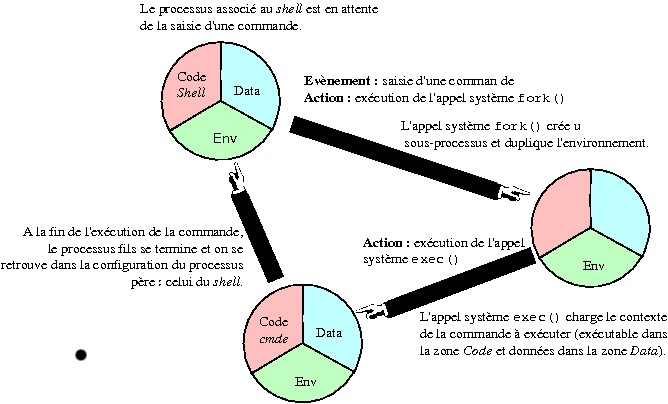
\includegraphics{./_Images/basic-notions/exec-cmd.jpg}
\caption{\label{fig-basnot-exec-cmd}Ex{\'e}cution d'une commande sous {\Unix}}
\end{figure}

L'appel syst{\`e}me "\texttt{fork()}" cr{\'e}e le processus et ne garde
que la zone m{\'e}moire "\texttt{ENV}". L'appel syst{\`e}me
"\texttt{exec()}" ex{\'e}cute la commande dans le processus cr{\'e}{\'e}.

\begin{remarque}
"\texttt{exec}" est aussi une commande du shell qui a la m{\^e}me fonctionnalit{\'e}.
\end{remarque}

La commande "\verb=% exec ls=" ex{\'e}cute "\texttt{ls}" dans le m{\^e}me processus
du shell (substitue le code du shell par le code de la commande "\texttt{ls}"
dans la zone m{\'e}moire "\texttt{CODE}" et s'arr{\^e}te d{\`e}s que son ex{\'e}cution est
termin{\'e}e. {\bf On est donc d{\'e}logg{\'e}}.

%%%%%%%%%%%%
\subsection{Les commandes de gestion des variables du shell}

\begin{definition}{Syntaxe}
\begin{tabular}{@{\hspace{1cm}}l}
	\texttt{set}\\[0.2cm]
	\texttt{variable=\textsl{valeur}}\\[0.2cm]
	\texttt{unset \textsl{variable}}\\[0.2cm]
	\texttt{export \textsl{variable}}\\[0.2cm]
	\texttt{printenv}\\[0.2cm]
	\texttt{env}\\
\end{tabular}
\end{definition}

\index{variable!gestion}
La commande \index{set@\texttt{set}}"\texttt{set}" sans argurments
affiche la liste des variables locales au shell

La commande \index{unset@\texttt{unset}}"\texttt{unset}" suivi d'un nom de variable permet
d'effacer celle-ci de la zone des variables locales du shell.

La commande \index{export@\texttt{export}}"\texttt{export}" suivie du nom d'une variable, permet de
placer une variable d{\'e}finie de la zone locale au shell vers la zone
d'environnement (exportation de la variable).

Les commandes \index{env@\texttt{env}}"\texttt{env}" et
\index{printenv@\texttt{printenv}}"\texttt{printenv}" listent les variables de la
zone d'environnement et les valeurs qui leur sont affect{\'e}es.

%%%%%%%%%%%
\subsection{Variables usuelles}

Le tableau \ref{tab-basnot-variables} donne la liste des
\index{variable!usuelle}variables les plus usuelles du shell {\Unix}.

\begin{longtable}{|l|p{8cm}|}
	\hline
	\multicolumn{2}{|r|}{Suite de la page pr{\'e}c{\'e}dente.} \\
	\hline
	\multicolumn{1}{|c|}{\textsl{Variable}}		&
	\multicolumn{1}{|c|}{\textsl{Signification}}	\\
	\hline
\endhead
	\hline
	\multicolumn{1}{|c|}{\textsl{Variable}}		&
	\multicolumn{1}{|c|}{\textsl{Signification}}	\\
	\hline
\endfirsthead
	\hline
\endfoot
	\hline
\endlastfoot
		\index{variable!PATH@\texttt{PATH}}\texttt{PATH}	&
		R{\'e}f{\'e}rence les chemins d'acc{\`e}s scrut{\'e}s lors de l'ex{\'e}cution d'une commande.\\
	\hline
		\index{variable!HOME@\texttt{HOME}}\texttt{HOME}	&
		R{\'e}f{\'e}rence le r{\'e}pertoire de \textsl{login}. C'est le r{\'e}pertoire par d{\'e}faut de la
		commande "\texttt{cd}".\\
	\hline
		\index{variable!PS1@\texttt{PS1}}\texttt{PS1}	&
		Invite du shell.\\
	\hline
		\index{variable!PS2@\texttt{PS2}}\texttt{PS2}	&
		Invite secondaire du shell. Lorsque vous demandez {\`a} ce qu'une commande se
		poursuive apr{\`e}s un retour chariot, c'est le contenu de cette de cette
		variable qui sera affich{\'e}.\\
	\hline
		\index{variable!LANG@\texttt{LANG}}\texttt{LANG}	&
		Langue utilis{\'e}e pour les messages.\\
	\hline
		\index{variable!HISTSIZE@\texttt{HISTSIZE}}\texttt{HISTSIZE}	&
		Nombre de commandes {\`a} m{\'e}moriser dans l'historique (Korn Shell uniquement).\\
	\hline
\caption{\label{tab-basnot-variables}Liste des variables les plus usuelles.}
\end{longtable}

%%%%%%%%%%%
\subsection{Visualisation d'une variable}

Pour rappeler le contenu d'une \index{variable!visualisation}variable
(locale ou d'environnement), il suffit de faire pr{\'e}c{\'e}der son nom
par le caract{\`e}re \index{\$@\texttt{\$}}"\texttt{\$}". Par cons{\'e}quent~:
\begin{itemize}
	\item pour r{\'e}f{\'e}rencer la variable, il suffit de pr{\'e}ciser son nom.
	\item pour r{\'e}f{\'e}rencer son contenu, il suffit de pr{\'e}ciser son nom pr{\'e}c{\'e}d{\'e} du
		  caract{\`e}re "\texttt{\$}".
\end{itemize}

\begin{example}
\begin{verbatim}
sh_ksh% my_var=schmoll
sh_ksh% echo $my_var
schmoll
\end{verbatim}
\end{example}

%%%%%%%%%%%%%%%%%%%%%%%%%%%%%%%%%%%%%%%%%%%%%%%%%%%%%%%%%%%%%%%%%%%%%
\section{\label{basicnot-exec}Ex{\'e}cution d'une commande}

La plupart des commandes sont des ex{\'e}cutables plac{\'e}s dans
\texttt{/bin}, \texttt{/sbin}, \texttt{/usr/bin}, \texttt{/usr/sbin},
etc. Ce sont des commandes {\Unix} ou
\index{commande!externe}\textbf{commandes externes au shell}. D'autres
commandes comme "\texttt{cd}", "\texttt{echo}",
"\texttt{pwd}" font partie intgrante de l'interpr{\'e}teur de commandes.
Ce sont des \index{commande!interne}\textbf{commandes internes au shell}.

Les commandes {\Unix} sont ex{\'e}cut{\'e}es dans un sous processus.
Comme les ex{\'e}cutables peuvent se trouver dans diff{\'e}rents
r{\'e}pertoires, le shell doit savoir o{\`u} les chercher. C'est la
variable "\index{variable!PATH@\texttt{PATH}}\texttt{PATH}" qui
d{\'e}finit a liste des r{\'e}pertoires {\`a} scruter et l'ordre dans
lequel le shell doit faire la recherche.

\begin{remarque}
Les commandes internes au shell ne sont pas ex{\'e}cut{\'e}es dans un processus fils.
\end{remarque}

%%%%%%%%%%%%%%%%%%%%%%%%%%%%%%%%%%%%%%%%%%%%%%%%%%%%%%%%%%%%%%%%%%%%%
\section{\label{redirect-io}Redirection des entr{\'e}es/sorties}

%%%%%%%%%%%
\subsection{Introduction}

Chaque processus sous {\Unix} poss{\'e}de trois canaux de communication~:
\begin{center}
\begin{tabular}{|l|c|c|c|}
	\hline
		\multicolumn{1}{|c|}{Canal de communication}	&
		Fichier											&
		Num{\'e}ro logique								&
		Analogie {\OpenVMS}								\\
	\hline \hline
		Entr{\'e}e standard								&
		\texttt{stdin}									&
		\texttt{0}										&
		\texttt{SYS\$INPUT}								\\
	\hline
		Sortie standard									&
		\texttt{stdout}									&
		\texttt{1}										&
		\texttt{SYS\$OUTPUT}							\\
	\hline
		Sortie d'erreurs standard						&
		\texttt{stderr}									&
		\texttt{2}										&
		\texttt{SYS\$ERROR}								\\
	\hline
\end{tabular}
\end{center}

La redirection de ces canaux est tr{\`e}s utilis{\'e}e sous {\Unix}. En
effet, beaucoup de commandes {\'e}crivent leur r{\'e}sultat par d{\'e}faut sur la
sortie standard (comme les filtres, par exemple). Le seul moyen de l'avoir
dans un fichier est de rediriger la sortie standard.
D'autres commandes lisent syst{\'e}matiquement sur leur entr{\'e}e standard
(comme les filtres). Si l'on veut qu'elles prennent un fichier comme
argument, il faudra rediriger l'entr{\'e}e standard.

Les syntaxes utilis{\'e}es pour les redirections sont explicit{\'e}es aux sections
\ref{basnot-stdin}, \ref{basnot-stdout} et \ref{basnot-stderr}.

%%%%%%%%%%%
\subsection{\label{basnot-stdin}Redirection de l'entr{\'e}e standard (\texttt{stdin})}

\begin{definition}{Syntaxe}
\begin{verbatim}
commande < nouvelle-entree-standard
\end{verbatim}
\end{definition}

Il est possible de rediriger l'entr{\'e}e de toute commande devant lire
des donn{\'e}es depuis \index{stdin@\texttt{stdin} (entr{\'e}e
standard)}l'entr{\'e}e standard, afin que la lecture se fasse sur un
fichier gr{\^a}ce au symbole \index{<@\verb=<=}"\verb=<=".

\begin{example}
\begin{verbatim}
% mail machin < fichier
\end{verbatim}
\end{example}

%%%%%%%%%%%%
\subsection{\label{basnot-stdout}Redirection de la sortie standard (\texttt{stdout})}

\begin{definition}{Syntaxe}
\begin{tabular}{l@{\hspace{1cm}}l}
	\verb=commande > nouvelle-sortie=	&	(Cr{\'e}ation/R{\'e}{\'e}criture)	\\
	\verb=commande >> nouvelle-sortie=	&	(Ajout)					\\
\end{tabular}
\end{definition}

Il est possible de rediriger la \index{stdout@\texttt{stdout} (sortie standard)}sortie
de toute commande devant {\'e}crire sur la sortie standard afin que l'{\'e}criture se fasse sur un fichier.
L'{\'e}criture peut se faire de deux fa\c{c}ons~:
\begin{itemize}
	\item	{\'e}criture dans un fichier et {\'e}crasement si le fichier existe d{\'e}j{\`a},
	\item	{\'e}criture {\`a} la suite d'un fichier d{\'e}j{\`a} existant.
\end{itemize}

Si une ligne de commande contient le symbole de redirection de la sortie
standard \index{>@\verb=>=}"\verb=>=" suivi d'un nom de fichier, celle-ci sera
redirig{\'e}e dans le fichier sp{\'e}cifi{\'e} au lieu du terminal. Deux cas peuvent
se pr{\'e}senter~:
\begin{itemize}
	\item	Si le fichier n'existe pas au moment o{\`u} la commande est ex{\'e}cut{\'e}e,
			il est cr{\'e}{\'e}.
	\item	Si le fichier existait, alors son contenu est {\'e}cras{\'e} par la sortie standard
			de la commande. Si on souhaite que celle-ci vienne s'ajouter {\`a} la suite,
			afin de pr{\'e}server son contenu initial, il suffit d'utiliser le double symbole
			"\verb=>>=". Dans le cas o{\`u} le fichier n'existait pas, il sera cr{\'e}{\'e}.
\end{itemize}

\begin{example}
\begin{verbatim}
% ls > fic
% date > who.log
% who >> who.log
\end{verbatim}
\end{example}

%%%%%%%%%%%%
\subsection{\label{basnot-stderr}Redirection de la sortie d'erreurs standard (\texttt{stderr})}

\begin{definition}{Syntaxe}
\begin{tabular}{l@{\hspace{1cm}}l}
	\verb=commande 2>fichier=	&	(Cr{\'e}ation/R{\'e}{\'e}criture)\\
	\verb=commande 2>>fichier=	&	(Ajout)\\
\end{tabular}
\end{definition}

La plupart des commandes {\Unix} produisent des messages de diagnostic
si un probl{\`e}me survient en cours d'ex{\'e}cution. La sortie des
messages d'erreur se fait sur la \index{stderr@\texttt{stderr} (sortie
d'erreurs standard)}sortie d'erreurs standard, qui, par d{\'e}faut, est
associ{\'e}e {\`a} l'{\'e}cran.

La sortie de messages d'erreur peut {\^e}tre redirig{\'e}e ind{\'e}pendamment de la
sortie standard. Ceci {\'e}vite d'avoir les messages d'ex{\'e}cution normale et
les messages de diagnostic entrelac{\'e}s dans un m{\^e}me fichier.

Pour rediriger la sortie d'erreurs standard dans un fichier, on utilise
les cha{\^\i}nes \index{>@\verb=>=}"\verb=2>=" et "\verb=2>>=" suivie du nom du fichier. Il ne doit
pas y avoir d'espace entre le "\texttt{2}" et le "\verb=>=". Comme pour la
redirection de la sortie standard, si le fichier n'existe pas, il est
cr{\'e}{\'e}, sinon il est {\'e}cras{\'e}. Si l'on veut que les messages de diagnostics
viennent s'ajouter en fin de fichier, il faut utiliser le double symbole
de redirection "\verb=2>>=".

\begin{example}
\begin{verbatim}
sh% cp fic1 fic2 2>fic
sh% cp fic1 fic2 2>>fic
\end{verbatim}
\end{example}

%%%%%%%%%%%
\subsection{Redirection d'une sortie standard vers une autre sortie standard}

Le principe reste identique. Il suffit de rediriger une sortie vers un
fichier (ou canal logique). Lorsque l'on veut r{\'e}f{\'e}rencer le canal
associ{\'e} {\`a} une sortie standard (idem pour l'entr{\'e}e et la sortie d'erreurs
standard) comme un fichier, il suffit de faire pr{\'e}c{\'e}d{\'e} son num{\'e}ro
logique par le caract{\`e}re <<\texttt{\&}".

Par exemple, si la \index{stderr@\texttt{stderr} (sortie d'erreurs
standard)}sortie d'erreurs standard doit {\^e}tre redirig{\'e}e vers la
\index{stdout@\texttt{stdout} (sortie standard)}sortie standard, il
suffira d'{\'e}crire~:
\begin{verbatim}
commande 2>&1
\end{verbatim}

Dans le cas o{\`u} la sortie standard et la sortie d'erreurs standard doivent {\^e}tre redirig{\'e}es
vers un m{\^e}me fichier, il faudra bien analyser le processus {\`a} mettre en jeu.

Dans le premier cas~:
\begin{center}
	\fbox{\texttt{commande 2>\&1 >fichier}}
\end{center}
le shell va ex{\'e}cuter les {\'e}tapes suivantes~:\\[0.5cm]
%	\epsfbox{_Images/basic-notions/stdout-stderr-1.eps}	\\
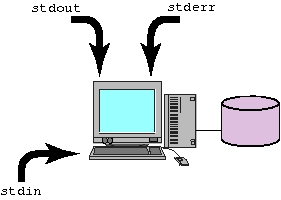
\includegraphics{./_Images/basic-notions/stdout-stderr-1.jpg}	\\
la sortie d'erreurs standard est redirig{\'e}e vers la valeur courante de la sortie 
standard, {\bf donc l'{\'e}cran}.\\[0.5cm]
%\epsfbox{_Images/basic-notions/stdout-stderr-2.eps}	\\
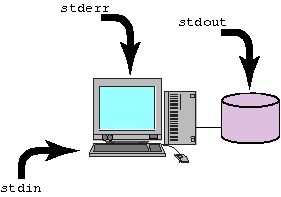
\includegraphics{./_Images/basic-notions/stdout-stderr-2.jpg} \\
la sortie standard vers un fichier. {\bf Donc seule la sortie standard a 
{\'e}t{\'e} redirig{\'e}e vers un fichier}.

Dans le deuxi{\`e}me cas~:
\begin{center}
	\fbox{\texttt{commande >fichier 2>\&1}}
\end{center}
le shell va ex{\'e}cuter les {\'e}tapes suivantes~:\\[0.5cm]
%	\epsfbox{_Images/basic-notions/stdout-stderr-2.eps}	\\
	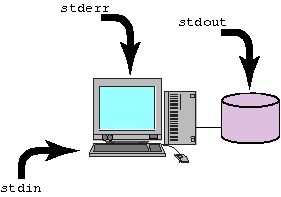
\includegraphics{./_Images/basic-notions/stdout-stderr-2.jpg}	\\
la sortie standard est redirig{\'e}e vers un fichier,\\[0.5cm]
%	\epsfbox{_Images/basic-notions/stdout-stderr-3.eps}	\\
	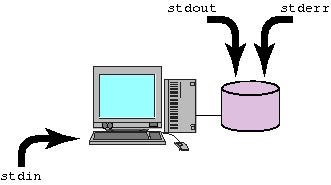
\includegraphics{./_Images/basic-notions/stdout-stderr-3.jpg}
la sortie d'erreurs standard est redirig{\'e}e vers la valeur courante sur laquelle
pointe la sortie standard, {\bf donc le fichier}. En cons{\'e}quence, 
{\bf la sortie standard et la sortie d'erreurs standard ont bien {\'e}t{\'e} redirig{\'e}es vers un 
m{\^e}me fichier}.

Le second mod{\`e}le est donc celui {\`a} retenir.

%%%%%%%%%%%%
\subsection{Redirection de la sortie standard d'une commande dans 
		l'entr{\'e}e standard d'une autre}

\begin{definition}{Syntaxe}
\begin{tabular}{ccc}
	\textsl{Commande A}				&	\texttt{|}	&	\textsl{Commande B}	\\
	Doit {\'e}crire sur \texttt{stdout}	&			&	Doit lire sur \texttt{stdin}\\
\end{tabular}
\end{definition}

Le symbole \index{|@\texttt{|}}"\texttt{|}" appel{\'e} \index{pipe}"\textsl{pipe}", est
utilis{\'e} pour relier deux commandes entre elles. La
\index{stdout@\texttt{stdout} (sortie standard)}sortie standard de la
commande {\`a} gauche du symbole "\texttt{|}" est utilis{\'e}e comme
\index{stdin@\texttt{stdin} (entr{\'e}e standard)}entr{\'e}e standard de
la commande de droite. La figure \ref{fig-basnot-out2in} illustre le
principe utilis{\'e} pour ce type de redirection.

\begin{figure}[hbtp]
	\centering
%	\epsfbox{_Images/basic-notions/out2in.eps}	\\
	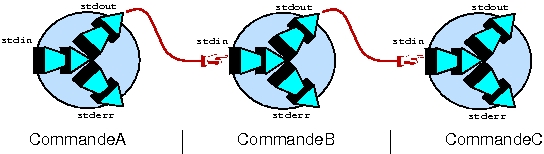
\includegraphics{./_Images/basic-notions/out2in.jpg}
	\caption{\label{fig-basnot-out2in}Enchainement de commandes, m{\'e}canisme du \textsl{pipe}.}
\end{figure}

C'est pourquoi~:
\begin{itemize}
	\item	toute commande situ{\'e}e {\`a} gauche du symbole "\texttt{|}" doit produire une
			sortie sur "\texttt{stdout}",
	\item	toute commande situ{\'e}e {\`a} droite du symbole "\texttt{|}" doit effectuer une
			lecture depuis "\texttt{stdin}",
	\item	toute commande entre les deux symboles "\texttt{|}" doit {\'e}crire sur
			"\texttt{stdout}" et lire sur "\texttt{stdin}". {\bf C'est donc un filtre}.
\end{itemize}

La redirection d'entr{\'e}e/sortie permet le passage d'informations entre un
processus et un fichier. Les \textsl{pipes} permettent le passage d'informations
entre processus. Ils constituent une solution pour utiliser la
sortie d'une commande en entr{\'e}e d'une autre commande sans passer par un
fichier interm{\'e}diaire.

{\Unix} repose sur le principe suivant. Chaque commande doit r{\'e}aliser
une seule chose. C'est la combinaison de ces commandes {\'e}l{\'e}mentaires,
gr{\^a}ce au m{\'e}canisme des \textsl{pipes} qui permet l'obtention de r{\'e}sultats
{\'e}labor{\'e}s.

%%%%%%%%%%%%%%%%%%%%%%%%%%%%%%%%%%%%%%%%%%%%%%%%%%%%%%%%%%%%%%%%%%%%%
\section{\label{basic-metacars}G{\'e}n{\'e}ration de noms de fichiers - Les m{\'e}tacaract{\`e}res}

%%%%%%%%%%%
\subsection{Introduction}

Les \index{m{\'e}tacaract{\`e}re}m{\'e}tacaract{\`e}res ne sont pas des
\index{wildcard}"\textsl{wildcards}". Un wildcard est
interpr{\'e}t{\'e} par une commande pour g{\'e}n{\'e}rer certains noms
de fichiers. Par contre les m{\'e}tacaract{\`e}res sont
interpr{\'e}t{\'e}s directement par le shell \textbf{avant
l'ex{\'e}cution de la commande}. Celle-ci re\c{c}oit des noms de
fichiers, comme si vous les aviez tap{\'e}s au clavier.

Les m{\'e}tacaract{\`e}res ne sont pas une aide {\`a} la frappe au clavier.
Les m{\'e}tacaract{\`e}res disponibles sont~:~\\
\begin{tabular}{lp{8cm}}
	\index{?@\texttt{?}}\texttt{?}		&
	Masque un caract{\`e}re, sauf le point en premi{\`e}re position.\\[0.5cm]
	\index{[]@\texttt{[]}}\texttt{[]}		&
	D{\'e}finit une classe de caract{\`e}res~:
	\begin{tabular}{lp{5cm}}
		\index{-@\texttt{-}}\texttt{-}	& pour d{\'e}finir une suite,\\
		\index{!@\texttt{!}}\texttt{!}	& pour exprimer une exclusion
	\end{tabular}
	Aucun s{\'e}parateur n'est utilis{\'e} pour exprimer une liste.\\[0.5cm]
	\index{*@\texttt{*}}\texttt{*}		&
	Masque toutes cha{\^\i}nes de caract{\`e}res, sauf le point en premi{\`e}re position.
\end{tabular}

\begin{remarque}
Les expressions utilisant les m{\'e}tacaract{\`e}res suivent les r{\`e}gles des expressions r{\'e}guli{\`e}res 
{\Unix}.
\end{remarque}

Les m{\'e}tacaract{\`e}res ne masquent jamais les fichiers cach{\'e}s. Le point en d{\'e}but du nom d'un 
fichier doit {\^e}tre tap{\'e} explicitement.

Le tableau \ref{tab-basenot-equiv-meta} donne les {\'e}quivalences entre {\Unix}
{\OpenVMS} et {\DOS} pour l'utilisation des m{\'e}tacaract{\`e}res sous {\Unix}.

\begin{table}[hbtp]
\centering
\begin{tabular}{|c|c|c|}
	\hline
		{\Unix}		&	{\OpenVMS}				&	{\DOS}		\\
	\hline \hline
		\texttt{*}	&	\texttt{*}				&	\texttt{*}				\\
	\hline
		\texttt{?}	&	\texttt{\%}				&	\texttt{?}				\\
	\hline
		\texttt{[]}	&	pas d'{\'e}quivalence	&	pas d'{\'e}quivalence	\\
	\hline
\end{tabular}
\caption{\label{tab-basenot-equiv-meta}\'{E}quivalence pour l'utilisation des m{\'e}tacaract{\`e}res
entre {\Unix}, {\OpenVMS} et {\DOS}.}
\end{table}

%%%%%%%%%%%
\subsection{Utilisation du m{\'e}tacaract{\`e}re "\texttt{?}"}

Le point d'interrogation \index{?@\texttt{?}}"\texttt{?}" masque un
et un seul caract{\`e}re sauf le point en premi{\`e}re position.

\begin{example}
\begin{tabular}{l@{\hspace{0.5cm}}p{8cm}}
	\texttt{echo ???}	&	Masque tous les noms de fichiers {\`a} trois caract{\`e}res.\\
	\texttt{ls A?C}	&	Masque tous les noms de fichiers {\`a} trois caract{\`e}res, dont
						le premier est "\texttt{A}" et le dernier est "\texttt{C}".\\
\end{tabular}
\end{example}

%%%%%%%%%%%
\subsection{Utilisation des m{\'e}tacaract{\`e}res "\texttt{[]}"}

Les crochets ouvrants et fermants
\index{[]@\texttt{[]}}\texttt{[]}"\texttt{[]}" d{\'e}finissent une
classe de caract{\`e}res, dont un et un seul sera masqu{\'e}.

\begin{example}
\begin{tabular}{l@{\hspace{0.5cm}}p{8cm}}
	\texttt{echo [abc]??}		&	Tous les fichiers dont le nom fait 3 caract{\`e}res et dont la
								premi{\`e}re lettre est soit "\texttt{a}", soit "\texttt{b}",
								soit "\texttt{c}".\\[0.5cm]
	\texttt{echo ?[a-zA-Z]}	&	Tous les fichiers dont le nom fait 2 caract{\`e}res et dont
								le dernier caract{\`e}re est une lettre (majuscule ou minuscule).
								\\[0.5cm]
	\texttt{echo [!a-zA-Z]??}	&	Tous les fichiers dont le nom fait 3 caract{\`e}res et dont le
								premier n'est pas une lettre.\\
\end{tabular}
\end{example}

%%%%%%%%%%%
\subsection{Utilisation du m{\'e}tacaract{\`e}re "\texttt{*}"}

L'{\'e}toile \index{*@\texttt{*}}"\texttt{*}" masque toute
cha{\^\i}ne de caract{\`e}res, m{\^e}me vide, sauf le point en
premi{\`e}re position.

\begin{example}
\begin{verbatim}
echo *
echo .*
echo *a*
\end{verbatim}
etc.
\end{example}

%%%%%%%%%%%%%%%%%%%%%%%%%%%%%%%%%%%%%%%%%%%%%%%%%%%%%%%%%%%%%%%%%%%%%
\section{\label{basic-quotes}Les quotes et les caract{\`e}res sp{\'e}ciaux}

\subsection{Introduction}

Nous avons vu dans les paragraphes pr{\'e}c{\'e}dents, les caract{\`e}res sp{\'e}ciaux suivants~:

\begin{longtable}{l@{\hspace{0.2cm}}p{8cm}}
	\texttt{\$}		&	utilis{\'e} pour la substitution d'une variable,						\\
	\texttt{? [] *}	&	utilis{\'e}s pour la g{\'e}n{\'e}ration des noms de fichiers par le Shell,		\\
	\verb=< > >>=	&	utilis{\'e}s pour la redirection des entr{\'e}es/sorties,					\\
	\spacekey		&	utilis{\'e} comme s{\'e}parateur par le Shell,								\\
	\texttt{|}		&	utilis{\'e} dans les \textsl{pipes}.										\\
\end{longtable}

Le contexte ne suffit pas toujours {\`a} d{\'e}terminer quel sens donner au
caract{\`e}re. C'est pourquoi il est n{\'e}cessaire d'avoir un moyen permettant
d'{\'e}chapper au sens sp{\'e}cial du caract{\`e}re et forcer celui-ci {\`a} {\^e}tre
consid{\'e}r{\'e} comme tel. \textbf{C'est le m{\'e}canisme de recours aux quotes}.

%%%%%%%%%%%%
\subsection{Les caract{\`e}res d'{\'e}chappements}

\begin{description}
	\item[\textbf{\index{\@$\mathtt{\backslash}$}back slash "$\mathtt{\backslash}$"}]\mbox{}\\
	Annule la signification particuli{\`e}re du caract{\`e}re imm{\'e}diatement apr{\`e}s.\\[0.5cm]
	\textsl{Exemple~:}\\
	\begin{tabular}{l@{\hspace{0.5cm}}p{6cm}}
		\verb=echo \$ABC=			&	renvoie la cha{\^\i}ne "\texttt{\$ABC}".\\
		\verb=echo abc \=\returnkey	&	annule l'interpr{\'e}tation du "\verb=<RETURN>=", il n'y a
										donc pas d'interpr{\'e}tation de la commande d'o{\`u} l'apparition d'un 
										"\textsl{prompt secondaire}" pour continuer la commande.\\
	\end{tabular}
	
	\item[\index{'@\texttt{'}}\textbf{simple quote "\texttt{'}"}]\mbox{}\\
	Annule l'interpr{\'e}tation de tous les caract{\`e}res {\`a} l'int{\'e}rieur des quotes {\`a} l'exception de la 
	simple quote elle-m{\^e}me.\\[0.5cm]
	\textsl{Exemple~:}\\
	\begin{tabular}{l@{\hspace{0.5cm}}p{6cm}}
		\verb=echo '$ABC > Bonjour'=	&	renvoie la cha{\^\i}ne "\verb=$ABC > Bonjour=" {\`a} l'{\'e}cran.\\
	\end{tabular}
	
	\item[\index{''@\texttt{''}}\textbf{doubles quotes "\texttt{"}"}]\mbox{}\\
		Annule l'interpr{\'e}tation de tous les caract{\`e}res entre les doubles quotes, {\`a} l'exception des 
		caract{\`e}res \verb=\=, \texttt{"}, \texttt{\$} et \texttt{`} (back quote).\\[0.5cm]
	\textsl{Exemple~:}\\
	\begin{tabular}{l@{\hspace{0.5cm}}p{6cm}}
		\texttt{ABC=Salut}	&	\\
		\verb=echo "$ABC > Bonjour"=	&
			\raisebox{2ex}[0pt]{renvoie la cha{\^\i}ne "\texttt{Salut > Bonjour}" {\`a} l'{\'e}cran.}\\
	\end{tabular}

\end{description}

%%%%%%%%%%%%
\subsection{R{\'e}sum{\'e}}

\begin{longtable}{|c|p{2.5cm}|p{5cm}|p{3cm}|}
	\hline
	\multicolumn{4}{|r|}{Suite de la page pr{\'e}c{\'e}dente.} \\
	\hline
	\multicolumn{1}{|c|}{Symbole}	&
	\multicolumn{1}{|c|}{Type}		&
	\multicolumn{1}{|c|}{Action}	&
	\multicolumn{1}{|c|}{Exception}	\\
	\hline
\endhead
	\hline
	\multicolumn{1}{|c|}{Symbole}	&
	\multicolumn{1}{|c|}{Type}		&
	\multicolumn{1}{|c|}{Action}	&
	\multicolumn{1}{|c|}{Exception}	\\
	\hline
\endfirsthead
	\hline
	\multicolumn{4}{|r|}{Suite page suivante $\cdots$} \\
	\hline
\endfoot
	\hline
\endlastfoot
	\index{\$@\texttt{\$}}\texttt{\$}	&	Caract{\`e}re sp{\'e}cial	&
		Substitue la valeur d'une variable.		&
		\multicolumn{1}{|c|}{\textsl{N.A.}}		\\
	\hline

	\index{>@\verb=>=}\verb=>=, \verb=>>=				&
		Caract{\`e}re sp{\'e}cial						&
		Redirige la sortie standard vers un fichier.	&
		\multicolumn{1}{|c|}{\textsl{N.A.}}				\\
	\hline

	\index{<@\verb=<=}\verb=<=	&	Caract{\`e}re sp{\'e}cial		&
		Redirige l'entr{\'e}e standard {\`a} partir d'un fichier.	&
		\multicolumn{1}{|c|}{\textsl{N.A.}}							\\
	\hline

	\index{|@\texttt{|}}\texttt{|}	&	Caract{\`e}re sp{\'e}cial	&
		Combine plusieurs commandes dans un \textsl{pipe}.			&
		\multicolumn{1}{|c|}{\textsl{N.A.}}							\\
	\hline

	\spacekey	&	Caract{\`e}re sp{\'e}cial	&
		D{\'e}limiteur dans une commande.		&
		\multicolumn{1}{|c|}{\textsl{N.A.}}		\\
	\hline

	\index{?@\texttt{?}}\texttt{?}	&	M{\'e}ta\-caract{\`e}re				&
		Masque un caract{\`e}re, sauf le point en premi{\`e}re position.	&
		\multicolumn{1}{|c|}{\textsl{N.A.}}									\\
	\hline

	\index{[]@\texttt{[]}}\texttt{[]}	&	M{\'e}ta\-caract{\`e}re		&
		D{\'e}finit une classe de caract{\`e}res {\`a} masquer.			&
		\multicolumn{1}{|c|}{\textsl{N.A.}}								\\
	\hline

	\index{*@\texttt{*}}\texttt{*}		&	M{\'e}ta\-caract{\`e}re	&
		Masque toutes cha{\^\i}nes de caract{\`e}res, sauf 
		le point en premi{\`e}re position.							&
		\multicolumn{1}{|c|}{\textsl{N.A.}}							\\
	\hline

	\index{\@$\mathtt{\backslash}$}\verb=\= (\textsl{back slash})	&
		Caract{\`e}re d'{\'e}chap\-pement						&
		Annule l'interpr{\'e}tation du caract{\`e}re suivant.	&
		\multicolumn{1}{|c|}{\textsl{Aucune.}} 			\\
	\hline
	
	\index{'@\texttt{'}}\texttt{'} (\textsl{simple quote})		&
		Caract{\`e}re d'{\'e}chap\-pement						&
		Annule l'interpr{\'e}tation de tous les caract{\`e}res
		entre les "\texttt{'}".								&
		\multicolumn{1}{|c|}{\textsl{Aucune.}} 					\\
	\hline

	\index{''@\texttt{''}}\texttt{"} (\textsl{double quotes})		&
		Caract{\`e}re d'{\'e}chap\-pement						&
		Annule l'interpr{\'e}tation de tous les caract{\`e}res
		entre les "\texttt{"}".								&
		\verb=\= (\textsl{back slash}), 
		"\texttt{\$}" (symbole dollar),
		"\texttt{"}" (double quotes),
		"\texttt{`}" (back quote).						\\
\end{longtable}

	%% Ok, index

%%%%%%%%%%%%%%%%%%%%%%%%%%%%%%%%%%%%%%%%%%%%%%%%%%%%%%%%%%%%%%%%%%%%%%%%
%                                                                      %
% This program is free software; you can redistribute it and/or modify %
% it under the terms of the GNU General Public License as published by %
% the Free Software Foundation; either version 2 of the License, or    %
% (at your option) any later version.                                  %
%                                                                      %
% This program is distributed in the hope that it will be useful,      %
% but WITHOUT ANY WARRANTY; without even the implied warranty of       %
% MERCHANTABILITY or FITNESS FOR A PARTICULAR PURPOSE.  See the        %
% GNU General Public License for more details.                         %
%                                                                      %
% You should have received a copy of the GNU General Public License    %
% along with this program; if not, write to the Free Software          %
% Foundation, Inc., 51 Franklin St, Fifth Floor, Boston,               %
% MA  02110-1301  USA                                                  %
%                                                                      %
%%%%%%%%%%%%%%%%%%%%%%%%%%%%%%%%%%%%%%%%%%%%%%%%%%%%%%%%%%%%%%%%%%%%%%%%
%
%	$Id$
%

\setcounter{remarque-cnt}{1}
\setcounter{example-cnt}{1}
\chapter{\label{multitask}Le mode multi-t{\^a}che}

%%%%%%%%%%%%%%%%%%%%%%%%%%%%%%%%%%%%%%%%%%%%%%%%%%%%%%%%%%%%%%%%%%%%%
\section{T{\^a}che de fond -- le {\sl background}}

\begin{definition}{Syntaxe}
\begin{tabular}{@{\hspace{1cm}}l}
	{\tt \% ligne-de-commande \&}\\[0.2cm]
	{\tt \% jobs}\\[0.2cm]
\end{tabular}
\end{definition}

Le caract{\`e}re \index{&@\texttt{\&}}"\verb=&=" permet
d'ex{\'e}cuter la commande en arri{\`e}re plan (\textsl{background}) et
permet de lancer pendant ce temps l{\`a} d'autres commandes en avant
plan. Lors de la d{\'e}connexion, tous les processes en arri{\`e}re plan
meurent. En effet, ils ne peuvent qu'exister que si leur p{\`e}re
existe.

Lorsqu'une commande est lanc{\'e}e en arri{\`e}re plan, le shell reporte
{\`a} l'utilisateur le num{\'e}ro de \index{PID@PID (\textsl{Process
IDentifier})}PID ({\sl Process IDentifier}) identifiant le processus
lanc{\'e} en arri{\`e}re plan avant de renvoyer le prompt. Une commande
s'ex{\'e}cutant en arri{\`e}re plan \textbf{ne peut pas} {\^e}tre
arr{\^e}t{\'e}e avec les touches \key{{\sc break}}, \control{C}, etc.
Par contre, une sortie de session (\textsl{logout}) tuera tous les
processus s'ex{\'e}cutant en arri{\`e}re plan.

Il est important qu'un processus lanc{\'e} en arri{\`e}re plan ait ses
entr{\'e}es/sorties redirig{\'e}es explicitement. Il est possible de
voir les processes lanc{\'e}s en arri{\`e}re plan avec la commande
\index{jobs@\texttt{jobs}} "\texttt{jobs}".
 
\begin{remarque}
\control{Z} {\bf ne sert pas {\`a} interrompre un process mais {\`a} le mettre
en attente en arri{\`e}re plan}. Si vous voulez interrompre une commande,
utilisez "\control{C}". Pour plus de renseignements sur les touches
d'interruption, reportez vous {\`a} la section \ref{multi-task-fg-bg}.
\end{remarque}

%%%%%%%%%%%%%%%%%%%%%%%%%%%%%%%%%%%%%%%%%%%%%%%%%%%%%%%%%%%%%%%%%%%%%
\section{\label{multi-task-backq}Substitution de commande - caract{\`e}re {\sl back quote}}

\begin{definition}{Syntaxe}
\begin{tabular}{@{\hspace{1cm}}l}
	{\tt `commande`}\\[0.2cm]
\end{tabular}
\end{definition}

La substitution de commande se fait en utilisant le caract{\`e}re back quote
("\index{`@\texttt{`}}\texttt{`}") pour lancer des commandes {\`a} ins{\'e}rer dans une cha{\^\i}ne de
caract{\`e}res.

La substitution de commandes dans une cha{\^\i}ne de caract{\`e}res est une autre
facilit{\'e} offerte par le shell. Elle permet de capturer la sortie d'une
commande et de l'assigner {\`a} une variable ou de l'utiliser comme un
argument d'une autre commande. Comme beaucoup de commandes {\Unix}
g{\'e}n{\`e}rent une sortie, la substitution de commandes peut {\^e}tre tr{\`e}s
int{\'e}ressante.

A propos de l'efficacit{\'e}, il est plus rapide, dans certains cas,
d'effectuer une substitution de commande plutot que de passer par une
redirection.

\begin{example}
\begin{verbatim}
% echo "my current shell is `basename $SHELL`"
% current_dir=`pwd`
% cd /etc
% cd $current_dir
\end{verbatim}
\end{example}

%%%%%%%%%%%%%%%%%%%%%%%%%%%%%%%%%%%%%%%%%%%%%%%%%%%%%%%%%%%%%%%%%%%%%
\section{Commandes associ{\'e}es}

%%%%%%%%%%%%
\subsection{\label{multi-task-kill}Commande "{\tt kill}"}

\begin{definition}{Syntaxe}
\begin{tabular}{@{\hspace{1cm}}l}
	{\tt kill [-sig\_no] PID [PID ...]}\\[0.2cm]
\end{tabular}
\end{definition}

La commande "\index{kill@\texttt{kill}}\texttt{kill}" peut {\^e}tre
utilis{\'e}e pour tuer n'importe quelle commande, y compris des
commandes lanc{\'e}es en arri{\`e}re plan. "{\tt kill}", plus
pr{\'e}cis{\'e}ment, envoie un signal aux processus d{\'e}sign{\'e}s.
L'action effectu{\'e}e par d{\'e}faut pour un process est de mourir sur
r{\'e}ception de certains signaux. Pour transmettre un signal {\`a} un
processus il faut en {\^e}tre le propri{\'e}taire; "{\tt kill}" ne
peut {\^e}tre utilis{\'e} pour tuer le process d'un autre utilisateur
{\`a} moins d'{\^e}tre le {\sl super user} (utilisateur "{\tt
root}").

Par d{\'e}faut "{\tt kill}" transmet le signal num{\'e}ro 15 au process sp{\'e}cifi{\'e}.
Dans le monde {\Unix}, il n'est pas possible de v{\'e}ritablement tuer un process
comme on pourrait le faire avec {\WindowsNT} et {\OpenVMS}. {\Unix}, en fait,
envoie une requ{\^e}te au processus pour qu'il se termine de lui-m{\^e}me. Il est
possible d'immuniser certaines commandes contre les signaux de terminaison. La
m{\'e}thode la plus efficace pour tuer un process est l'utilisation du signal 9.

Pour avoir la liste des signaux et leur action, reportez-vous {\`a} "{\tt signal(2)}".

\begin{example}
\begin{verbatim}
% cat /usr/man/man1/* >big.file &
[[1] 1234
% kill 1234
[1] + Terminated	cat /usr/man/man1/* >big.file
\end{verbatim}
\end{example}

%%%%%%%%%%%%
\subsection{Commande "{\tt wait}"}

\begin{definition}{Syntaxe}
\begin{tabular}{@{\hspace{1cm}}l}
	{\tt wait [PID]}\\[0.2cm]
\end{tabular}
\end{definition}

La commande "\index{wait@\texttt{wait}}\texttt{wait}" permet de
suspendre l'ex{\'e}cution d'un shell script jusqu'{\`a} ce que le
processus, dont le \index{PID@PID (\textsl{Process IDentifier})}\textsl{PID}
est sp{\'e}cifi{\'e} en argument, se termine. Si aucun \textsl{PID} n'est
sp{\'e}cifi{\'e}, on attendra, dans ce cas, que tous les processus lanc{\'e}s
en arri{\`e}re plan soient termin{\'e}s.

\begin{example}
\begin{verbatim}
% cat /usr/man1/* >big.file &
% find / -print >big.file2 &
% wait
% echo "cat et find sont termin{\'e}s ..."
\end{verbatim}
\end{example}

%%%%%%%%%%%%
\subsection{\label{multi-task-fg-bg}Les commandes "{\tt fg}" et "{\tt bg}"}

\begin{definition}{Syntaxe}
\begin{tabular}{@{\hspace{1cm}}l@{\hspace{1cm}}l}
	{\tt bg PID}				&	{\tt bg} = back ground (arri{\`e}re plan)	\\
	{\tt bg \% num{\'e}ro}			&	\\[0.2cm]
	{\tt fg PID}				&	{\tt fg} = foreground (avant plan)		\\
	{\tt fg \% num{\'e}ro}			&	\\[0.2cm]
\end{tabular}
\end{definition}

Nous avons vu qu'avec la touche "\control{Z}", il {\'e}tait possible de
faire passer une commande \textbf{en attente} en arri{\`e}re plan. {\large
L'ex{\'e}cution est suspendue mais le process est toujours actif}. Si vous
d{\'e}sirez qu'elle continue {\`a} s'ex{\'e}cuter, toujours en arri{\`e}re plan,
utilisez la commande "\index{bg@\texttt{bg}}{\tt bg}".

Pour refaire passer en avant plan une commande qui s'ex{\'e}cute en arri{\`e}re
plan utiliser la commande "\index{fg@\texttt{fg}}{\tt fg}". "\texttt{fg}"
permet aussi de r{\'e}activ{\'e} une commande suspendue par "\control{Z}".
Le processus associ{\'e} devient alors le processus courant jusqu'{\`a} ce que
cette commande soit achev{\'e}e.

Pour plus de renseignements, reportez vous {\`a} "\texttt{sh(1)}".

\begin{example}
\begin{verbatim}
% find / -print >/dev/null
\end{verbatim}
\control{Z}
\begin{verbatim}
[1] 1234 Suspended
% bg %1
[1] 1234 find / -print >/dev/null &
% ls
\end{verbatim}
$\cdots$\\
\begin{verbatim}
%fg %1
find / -print >/dev/null
\end{verbatim}
\end{example}

\begin{definition}{\'{E}quivalence}
\begin{tabular}{|l|l|}
	\hline
		\multicolumn{1}{|c|}{{\Unix}}	&
		\multicolumn{1}{|c|}{{\OpenVMS}}	\\
	\hline \hline
		\control{Z}	&	{\tt SET PROCESS/SUSPEND}	\\
	\hline
		{\tt fg}		&	{\tt RESUME}				\\
	\hline
		{\tt bg}		&	Pas d'{\'e}quivalence.			\\
	\hline
\end{tabular}
\end{definition}

%%%%%%%%%%%%
\subsection{Commandes "{\tt at}"}

\begin{definition}{Syntaxe}
\begin{tabular}{@{\hspace{0.5cm}}l}
	{\tt at [-c | -s | -k] [-m] [-q queuename] [-f file]} \\
	\hspace{1cm}{\tt date [increment] [command | file]}\\[0.2cm]
	{\tt at -r job\_number ...}\\[0.2cm]
	{\tt at -l [-q queuename] [user ...]}\\[0.2cm]
\end{tabular}
\end{definition}

La commande "\index{at@\texttt{at}}\texttt{at}" permet de diff{\'e}rer
l'ex{\'e}cution de travaux. Elle lit sur son entr{\'e}e standard les commandes
qu'elle doit lanc{\'e} {\`a} la date sp{\'e}cifi{\'e}e.

Au lieu d'envoyer les ordres {\`a} ex{\'e}cuter sur l'entr{\'e}e standard, vous pouvez~:
\begin{itemize}
	\item	sp{\'e}cifier directement la commande {\`a} la suite. Dans ce cas, l'entr{\'e}e standard
			de la commande qui aura {\'e}t{\'e} saisie, devra {\^e}tre prise {\`a} partir d'un fichier
			avec les m{\'e}canismes d{\'e}crits {\`a} la section \ref{basnot-stdin}.
	\item	donner le nom d'un fichier contenant les commandes {\`a} ex{\'e}cuter. Celui-ci n'est pas
			lu {\`a} la place de l'entr{\'e}e standard mais est trait{\'e} comme une proc{\'e}dure de commande.
			Il doit donc {\^e}tre accessible en ex{\'e}cution par le Shell (cf. sections
			\ref{cmds-protect} et \ref{basicnot-exec}).
\end{itemize}

La commande "\index{batch@\texttt{batch}}\texttt{ batch}" ex{\'e}cute les travaux seulement lorsque le
niveau de la charge du syst{\`e}me le permet. La commande "\texttt{at}"
redirige automatiquement sa sortie standard et sa sortie d'erreurs
standard dans la boite aux lettres du courrier {\'e}lectronique. Par d{\'e}faut,
la commande "\texttt{at}" utilise le Bourne Shell comme interpr{\'e}teur de
commandes. Si vous d{\'e}sirez changer l'interpr{\'e}teur de commande par
d{\'e}faut, les options suivantes devront {\^e}tre sp{\'e}cifi{\'e}es~:
\begin{center}
\begin{tabular}{|l|l|}
	\hline
		\multicolumn{1}{|c|}{Option}		&
		\multicolumn{1}{|c|}{Shell}			\\
	\hline \hline
		"{\tt -c}"	&	C Shell			\\
	\hline
		"{\tt -k}"	&	Korn Shell		\\
	\hline
\end{tabular}
\end{center}

Le param{\`e}tre "{\tt date}" a le format suivant~:
\begin{center}
{\tt [[CC]AA]MMJJhhmm[.ss]}
\end{center}
avec~:\\
\begin{tabular}{@{\hspace{0.2cm}}l@{\hspace{0.2cm}}l}
	{\tt CC}	&	les deux chiffres des centaines de l'ann{\'e}e,	\\
	{\tt AA}	&	les deux derniers chiffres de l'ann{\'e}e,		\\
	{\tt MM}	&	le mois (01-12),							\\
	{\tt JJ}	&	le jour (01-31),							\\
	{\tt hh}	&	l'heure (00-23),							\\
	{\tt mm}	&	les minutes (00-59),						\\
	{\tt ss}	&	les secondes (00-59).						\\
\end{tabular}

"{\tt CC}" et "{\tt AA}" sont optionnels, l'ann{\'e}e en cours est prise par d{\'e}faut.

Le param{\`e}tre "{\tt date}" admet aussi les formats suivants~:
\begin{itemize}
	\item	La commande "{\tt at}" interpr{\`e}te les valeurs compos{\'e}es d'un ou deux chiffres
			comme {\'e}tant des heures. Elle interpr{\`e}te les valeurs compos{\'e}es de quatre chiffres
			comme {\'e}tant des heures et des minutes. Vous pouvez {\'e}ventuellement s{\'e}parer les heures
			des minutes par le caract{\`e}re deux points "{\tt :}". Dans ce cas, le format sera
			"{`}{\tt hh:mm}>.
	\item	Vous pouvez indiquer le suffixe "{\tt am}", "{\tt pm}" ou "{\tt zulu}".
			Si vous ne sp{\'e}cifiez ni "{\tt am}" ni "{\tt pm}", la commande "{\tt at}"
			utilise une horloge de 24 heures. Si vous sp{\'e}cifiez "{\tt zulu}", le temps 
			universel\footnote{LE temps universel correspond au fuseau horaire de Greenwich.}
			est utilis{\'e}.
	\item	L'un des mots clefs suivants~:
		\begin{itemize}
			\item[$\star$]	"{\tt noon}" pour {\sl midi},
			\item[$\star$]	"{\tt midnight}" pour {\sl minuit},
			\item[$\star$]	"{\tt now}" pour repr{\'e}senter l'instant pr{\'e}sent,
			\item[$\star$]	"{\tt A}" en abr{\'e}viation de "{\tt am}",
			\item[$\star$]	"{\tt P}" en abr{\'e}viation de "{\tt pm}", 
			\item[$\star$]	"{\tt N}" en abr{\'e}viation de "{\tt noon}",
			\item[$\star$]	"{\tt M}" en abr{\'e}viation de "{\tt midnight}".
		\end{itemize}
\end{itemize}

\begin{remarque}
	Le mot clef "{\tt now}" peut {\^e}tre utilis{\'e} uniquement si vous indiquez le param{\`e}tre
	"{\tt date}" ou "{\tt increment}". Dans le cas contraire, le message 
	"{\tt too late}" s'affiche.
\end{remarque}

Le param{\`e}tre "{\tt date}" permet d'indiquer un nom de mois et un
num{\'e}ro de jour ({\'e}ventuellement un num{\'e}ro d'ann{\'e}e pr{\'e}c{\'e}d{\'e} d'une virgule),
ou un jour de la semaine. La commande "{\tt at}" reconna{\^\i}t deux
jours particuliers~: il s'agit de "{\tt today}" et de "{\tt
tomorrow}". Si l'heure indiqu{\'e}e est post{\'e}rieure {\`a} l'heure d'entr{\'e}e de
la commande, "{\tt today}" est utilis{\'e}e par d{\'e}faut en tant que
param{\`e}tre "{\tt date}". Dans le cas contraire, celui-ci prend la
valeur "{\tt tomorrow}". Si vous indiquez un mois ant{\'e}rieur {\`a} celui
en cours sans pr{\'e}ciser d'ann{\'e}e, l'ann{\'e}e suivante est utilis{\'e}e par
d{\'e}faut.

Le param{\`e}tre facultatif "{\tt increment}" peut prendre l'une des 
valeurs suivantes~:
\begin{itemize}
	\item	le signe plus "{\tt +}" suivi d'un nombre et de l'un des mots suivants~:
			"{\tt minute[s]}", "{\tt hour[s]}", "{\tt day[s]}", "{\tt week[s]}",
			"{\tt month[s]}" ou "{\tt year[s]}" (ou tout {\'e}quivalent en anglais).
	\item	le mot "{\tt next}" suivi de l'un des mots suivants~: "{\tt minute[s]}",
			"{\tt hour[s]}", "{\tt day[s]}", "{\tt week[s]}",
			"{\tt month[s]}" ou "{\tt year[s]}" (ou tout {\'e}quivalent en anglais).
\end{itemize}

\begin{definition}{Options}
\begin{tabular}{@{\hspace{0.2cm}}l@{\hspace{0.2cm}}p{6cm}}
	{\tt -c}					&	Indique que le C Shell sera utilis{\'e} pour ex{\'e}cuter
									le travail.\\[0.2cm]
	{\tt -k}					&	Indique que le Korn Shell sera utilis{\'e} pour ex{\'e}cuter le
									travail.\\[0.2cm]
	{\tt -l}					&	Liste les travaux {\`a} ex{\'e}cuter.\\[0.2cm]
	{\tt -m}					&	Envoie un message {\`a} l'utilisateur apr{\`e}s l'ex{\'e}cution de
									la commande.\\[0.2cm]
	{\tt -q} {\sl  queuename}	&	Sp{\'e}cifie la file d'attente dans laquelle on effectue le
									travail.\\[0.2cm]
	{\tt -s}					&	Indique que le Bourne Shell sera utilis{\'e} pour ex{\'e}cuter
									le travail.\\[0.2cm]
	{\tt -r} {\sl job}			&	Supprime des travaux programm{\'e}s par la commande
									"{\tt at}" (le param{\`e}tre "{\tt job}" correspond
									{\`a} un num{\'e}ro affect{\'e} par la commande).\\
\end{tabular}
\end{definition}

Par d{\'e}faut, l'attribution des files d'attente se fait de la fa\c{c}on suivante~:\\
\begin{tabular}{|c|p{6cm}|}
	\hline
	file d'attente	&	type de travaux \\
	\hline \hline
	{\tt a}		&	travaux soumis avec la commande "{\tt at}".\\
	{\tt b}		&	travaux "{\sl batch}".\\
	{\tt c}		&	travaux soumis par le "{\sl cron}".\\
	{\tt d}		&	travaux "{\sl sync}".\\
	{\tt e}		&	travaux Korn Shell.\\
	{\tt f}		&	travaux C Shell.\\
	\hline
\end{tabular}

\begin{remarque}
Les travaux "{\sl batch}" sous {\Unix} ont un sens diff{\'e}rent de celui
habituellement entendu sous {\OpenVMS}. Ceux-ci ne sont ex{\'e}cut{\'e}s seulement
si le syst{\`e}me dispose de suffisamment de ressources. Avec {\OpenVMS}, il est possible
d'affecter un niveau de priorit{\'e} des processus pris en compte par l'ordonnanceur du
syst{\`e}me ({\sl scheduler}). Il est donc possible d'avoir une file d'attente offrant
un niveau bas de ressource (priorit{\'e} faible), les travaux ne seront donc ex{\'e}cut{\'e}s
seulement si le syst{\`e}me dispose de suffisamment de ressources. Par contre, il est
aussi possible d'avoir une file d'attent avec un niveau {\'e}lev{\'e}. Dans ce cas, les travaux
passeront en priorit{\'e}. Ceci peut {\^e}tre utile en fonction de l'environnement
d'exploitation.
\end{remarque}

Pour plus de renseignements, reportez-vous {\`a} "{\tt at(1)}".

\begin{example}
Pour programmer l'ex{\'e}cution d'une commande {\`a} partir du terminal, entrez une commande 
semblable {\`a} l'un des exemples suivants.\\
Si "{\tt uuclean}" se trouve dans le r{\'e}pertoire courrant (ou dans un r{\'e}pertoire sp{\'e}cifi{\'e} dans la 
variable "{\tt PATH}")~:
\begin{verbatim}
% at 5 pm Friday uuclean
% at now next week uuclean
\end{verbatim}
Si "{\tt uuclean}" se trouve dans le r{\'e}pertoire "\verb=$HOME/bin/uuclean="~:
\begin{verbatim}
% at now + 2 days $HOME/bin/uuclean
% at now + 2 days
$HOME/bin/uuclean
\end{verbatim}
\control{D}
\end{example}

\begin{remarque}
Lorsque vous indiquez, sur la ligne de commande, un nom de commande
comme dernier {\'e}l{\'e}ment, vous devez sp{\'e}cifier le chemin d'acc{\`e}s complet si
celle-ci ne se trouve pas dans le r{\'e}pertoire courrant. En outre, la
commande "{\tt at}" ne prend en compte aucun argument pour les
commandes {\`a} lancer.
\end{remarque}

\begin{example}
Pour ex{\'e}cuter la commande "{\tt uuclean}" le 24 Janvier {\`a} 15 heures, entrez l'une des 
commandes ci-dessous~:
\begin{verbatim}
% echo uuclean | at 3:00 pm January 24
% echo uuclean | at 3pm Jan 24
% echo uuclean | at 1500 jan 24
\end{verbatim}
\end{example}

\begin{definition}{\'{E}quivalence}
\begin{center}
\begin{tabular}{|c|c|}
	\hline
		{\Unix}		&	{\OpenVMS}			\\
	\hline \hline
		{\tt at}		&	{\tt submit}			\\
	\hline
\end{tabular}
\end{center}
\end{definition}

%%%%%%%%%%%%%%%%%%%%%%%%%%%%%%%%%%%%%%%%%%%%%%%%%%%%%%%%%%%%%%%%%%%%%
\section{R{\'e}p{\'e}tition de t{\^a}ches~: {\tt crontab}}

%%%%%%%%%%%%
\subsection{Introduction -- Syntaxe}

\index{crontab}{\sl crontab}�st un utilitaire utilis{\'e} pour ex{\'e}cuter un certain nombre de t{\^a}ches
r{\'e}p{\'e}titives. Chaque utilisateur poss{\`e}de sa propre table de t{\^a}ches. Celle-ci est
enregistr{\'e}e dans un r{\'e}pertoire du syst{\`e}me d'exploitation (<<{\tt /var/spool/crontab}").

Cette fonctionnalit{\'e} du syst{\`e}me est associ{\'e} {\`a}~:
\begin{itemize}
	\item	la commande "{\tt crontab}",
	\item	un fichier de description des t{\^a}ches {\`a} effectuer.
\end{itemize}

La commande {\tt crontab} ob{\'e}it {\`a} la syntaxe explicit{\'e}e ci-apr{\`e}s.

\begin{definition}{Syntaxe}
{\tt crontab [ -u {\sl user} ] {\sl file}}\\
{\tt crontab [ -u {\sl user} ] \{ -l | -r | -e \}}
\end{definition}

Le premier format de la commande permet d'enregistrer les commandes {\`a} effectuer .
Le second format permet de consulter et de maintenir la table de description des
t{\^a}ches.
Les options disponibles sont~:
\begin{description}
	\item[{\tt -u user}]\mbox{}\\
		L'option "{\tt -u {\sl user}}" permet de pr{\'e}ciser pour  quel utilisateur, d{\'e}fini
		sur le syst{\`e}me, les op{\'e}rations sont {\`a} effectuer. Par d{\'e}faut, la commande
		{\tt crontab} concernera votre propre table de description.
		
	\item[{\tt -l}]\mbox{}\\
		L'option "{\tt -l}" affiche le contenu de la table de description de
		l'utilisateur concern{\'e} sur la sortie standard.
		
	\item[{\tt -r}]\mbox{}\\
		L'option "{\tt -r}" r{\'e}initialise la table de description de l'utilisateur
		concern{\'e}~: toutes les t{\^a}ches qui y sont d{\'e}finies seront supprim{\'e}es.
		
	\item[{\tt -e}]\mbox{}\\
		L'option "{\tt -e}" permet d'{\'e}diter la table de description de l'utilisateur
		concern{\'e}. L'{\'e}diteur utilis{\'e} sera celui pr{\'e}cis{\'e} par le contenu de la variable
		d'environnement "{\tt EDITOR}" ou bien la variable d'environnement
		"{\tt VISUAL}". Les modifications prendont effet imm{\'e}diatement apr{\`e}s la sortie
		de l'{\'e}diteur de texte. 
\end{description}

Pour plus de pr{\'e}cisions, reportez-vous {\`a} {\tt crontab(1)}.

%%%%%%%%%%%%
\subsection{Fichier de description de t{\^a}ches}

Le fichier de description des t{\^a}ches va contenir les instructions
n{\'e}cessaires au processus de supervision (processus "{\tt
cron(8)}"). Celui d{\'e}crira les op{\'e}rations de la fa\c{c}on suivante "{\sl
ex{\'e}cute cette commande {\`a} cette heure l{\`a} ce jour-ci}".

Dans ce fichier,
\begin{itemize}
	\item	toute ligne commen\c{c}ant par le caract{\`e}re "\verb=#=" est ignor{\'e}e (ligne
			de commentaires),
	\item	les lignes blanches sont ignor{\'e}es,
	\item	les espaces et les tabulations en d{\'e}but de ligne sont ignor{\'e}s.
\end{itemize}

\begin{remarque}
Il n'est pas possible de mettre des commentaires au milieu d'une ligne. Le signe de
commentaire doit donc {\^e}tre le premier caract{\`e}re de la ligne.
\end{remarque}

Chaque ligne de description, hormis les lignes de commentaires, peuvent , soit
d{\'e}finir des variables d'environnement pour l'ensemble des t{\^a}ches {\`a} effectuer,
soit des commandes {\`a} ex{\'e}cuter aux instants sp{\'e}cifi{\'e}s. La d{\'e}finition d'une
variable d'environnement dans le fichier ob{\'e}it {\`a} la syntaxe suivante~:
\begin{quote}
{\tt {\sl nom} = {\sl valeur}}
\end{quote}
o{\`u} "{\sl nom}" repr{\'e}sente le nom de la variable d'environnement et "{\sl
valeur}" repr{\'e}sente la valeur qui lui est affect{\'e}e. Les espaces de part et
d'autre du signe {\sl {\'e}gual} "{\tt =}" sont optionnels. Si la valeur {\`a}
affecter {\`a} la variable est une chaine de caract{\`e}res, il est pr{\'e}f{\'e}rable de la
mettre entre simple quotes ("{\tt '}"�u double quotes ("\verb="=").

{\bf Pour toutes les commandes qui seront ex{\'e}cut{\'e}es~:
\begin{itemize}
	\item	leur sortie standard et leur sortie d'erreur standard redirig{\'e}es vers
			la boite aux lettres de l'utilisateur,
	\item	leur entr{\'e}e standard devra {\^e}tre explicitement pr{\'e}cis{\'e}e si cela est
			nec{\'e}ssaire.
\end{itemize}
}

Certaines variables d'environnement sont automatiquement positionn{\'e}es par le
gestionnaire de t{\^a}ches {\tt cron(8)}~:\\
\begin{tabular}{|c|p{8cm}|}
	\hline
	\multicolumn{1}{|c|}{Variable}	&	\multicolumn{1}{|c|}{Description} \\
	\hline \hline
	{\tt SHELL}		&	repr{\'e}sente l'interpr{\'e}teur de commande par d{\'e}faut. Cette variable est initialis{\'e}e {\`a}
					"{\tt /bin/sh}", donc le Bourne Shell.\\
	\hline
	{\tt LOGNAME}	&	repr{\'e}sente le nom de connexion de l'utilisateur. Par d{\'e}faut, elle
					correspond {\`a} votre entr{\'e}e dans la base des utilisateurs.\\
	\hline
	{\tt USER}		&	a exactement les m{\^e}mes fonctionnalit{\'e}s que la variable "{\tt LOGNAME}". Cependant,
					certains utilitaires issus des syst{\`e}mes BSD\footnote{comme SunOS 4 et Ultrix.} utilisent
					"{\tt USER}" plut{\^o}t que "{\tt LOGNAME}".\\
	\hline
	{\tt HOME}		&	repr{\'e}sente votre r{\'e}pertoire de connexion. Par d{\'e}faut, il correspond {\`a} celui
					d{\'e}fini dans les caract{\'e}ristiques de l'utilisateur.\\
	\hline
	{\tt MAILTO}	&	En plus des variables {\tt LOGNAME}, {\tt HOME} et {\tt SHELL},
					le processus "{\tt cron(8)}" examine le contenu de la variable
					d'environnement "{\tt MAILTO}" afin de savoir s'il est n{\'e}cessaire
					d'envoyer un message donnant le r{\'e}sultat de l'ex{\'e}cution des commandes.
					Si cette variable est d{\'e}finie et non vide, elle doit contenir l'adresse
					courrier de la personne {\`a} qui envoyer les messages. Si elle est d{\'e}finie
					{\bf mais vide}\footnote{Dans ce cas la variable est initialis{\'e}e avec
					la chaine vide de la fa\c{c}on suvante~: ":MAILTO="":".}, aucun
					message ne sera envoy{\'e}.\\
					&	Au cas o{\`u} aucune option se serait pr{\'e}cis{\'e} gr{\^a}ce {\`a} la variable
					"{\tt MAILTO}", le r{\'e}sultat produit sur la sortie standard
					est envoy{\'e} dans la boite aux lettres de l'utilisateur poss{\'e}dant
					cette liste de t{\^a}ches {\`a} ex{\'e}cuter.\\
	\hline
\end{tabular}

\begin{remarque}
Cette fonctionnanlit{\'e} offerte gr{\^a}ce {\`a} la variable "{\tt MAILTO}" peut {\^e}tre
tr{\`e}s utile si vous d{\'e}cidez d'utiliser un autre serveur de messagerie que
"{\tt /usr/lib/sendmail}". Dans ce cas, "{\tt /bin/mail}" sera employ{\'e}
pour assurer l'acheminement des messages. "{\tt /bin/mail}" n'utilisera
pas la notion d'{\sl aliases} de "{\tt /usr/lib/sendmail}".
\end{remarque}

Les lignes de description de t{\^a}ches se composent de plusieurs champs s{\'e}par{\'e}s
par des espaces ou tabulations. Chaque ligne poss{\`e}de~:
\begin{itemize}
	\item	cinq champs pr{\'e}cisant la date et l'heure {\`a} laquelle la commande
			doit {\^e}tre lanc{\'e}e,
	\item	dans le cas o{\`u} la table de description est celle de l'administrateur,
			le nom de l'utilisateur pour lequel on lance la commande\footnote{Cette
			fonctionnalit{\'e} n'est pas disponible sur tous les {\Unix}. On la trouvera
			par exemple sous {\Linux}.},
	\item	la commande {\`a} lancer.
\end{itemize}
Le service "{\tt cron(8)}"\footnote{"{\tt cron(8)}"
est un processus syst{\`e}me s'ex{\'e}cutant en permanence. Dans le jargon {\Unix}, un
tel processus est appel{\'e} "{\sl d{\'e}mon}" ou "{\sl daemon}".} examine toutes les
minutes, les tables de description. Lorsque la date pr{\'e}cis{\'e}e dans une entr{\'e}e 
d'une table de description de t{\^a}ches, le service "{\tt cron(8)}" cr{\'e}e un sous
processus sous l'identit{\'e} de la personne et lance la commande {\`a} l'int{\'e}rieur
de ce contexte. La sp{\'e}cification de la date et de l'heure se compose
des cinq informations suivantes~:\\[0.5cm]
\begin{tabular}{|l|l|}
	\hline
	\multicolumn{1}{|c|}{Champ}	&	\multicolumn{1}{|c|}{Valeurs autoris{\'e}es}	\\
	\hline
	minute				&	0-59 \\
	heure				&	0-23 \\
	jour du mois		&	1-31 \\
	mois				&	1-12 \\
	jour de la semaine	&	0-7\footnote{0 ou 7 repr{\'e}sente "{\sl dimanche}")}\\
	\hline
\end{tabular}

Si l'un de ces champs contient le caract{\`e}re "\verb=*=", celui-ci ne
doit pas {\^e}tre pris en compte, ou bien l'une des bornes inf{\'e}rieure ou sup{\'e}rieure
doit {\^e}tre consid{\'e}r{\'e}e dans la d{\'e}termination de la date. Par exemple~:\\[0.5cm]
\begin{tabular}{|l|@{\hspace{0.2cm}indique~:~}p{8cm}|}
	\hline
	{\tt 0 1 * * *}	&	"{\sl tous les jours {\`a} 01:00}"\\
	{\tt 0 0 * * 1}	&	"{\sl tous les lundis {\`a} minuit}"\\
	{\tt * * * 2 3}	&	"{\sl tous les mardis du mois de f{\'e}vrier {\`a} minuit}"\\
	\hline
\end{tabular}

Pour chaque champ, il est possible de donner~:
\begin{itemize}
	\item	une s{\'e}quence de nombres s{\'e}par{\'e}s par des virgules,
	\item	des plages de nombre, en sp{\'e}cifiant les bornes inf{\'e}rieurs et sup{\'e}rieures
			s{\'e}par{\'e}es par le caract{\`e}re "{\tt -}",
	\item	de combiner les deux possibilit{\'e}s.
\end{itemize}

\begin{example}
\begin{tabular}{|l|@{\hspace{0.2cm}correspond {\`a} la s{\'e}quence ~:~}p{3cm}|}
	\hline
	{\tt 1,5}		&	"{\sl 1, 5}"\\
	{\tt 8-10}		&	"{\sl 8, 9, 10}"\\
	{\tt 0-5,7,9}	&	"{\sl 0, 1, 2, 3, 4, 5, 7, 9}"\\
	{\tt 0-4,8-12}	&	"{\sl 0, 1, 2, 3, 4, 8, 9, 10, 11, 12}"\\
	\hline
\end{tabular}
\end{example}

\begin{remarque}
Aucun espace ne doit {\^e}tre introduit dans les cinq champs associ{\'e}s {\`a} la date et 
{\`a} l'heure de lancement d'une commande.
\end{remarque}

\begin{remarque}
Certaines extensions du service "{\tt cron(8)}" permettent
de modifier l'incr{\'e}ment des plages de nombres. Une plage de nombres suivie de
"\verb=/<number>=>> indique le pas entre les valeurs {\`a} prendre {\`a} l'int{\'e}rieur
de l'intervalle. Par exemple, "\verb=0-23/2=", dans le champ <<{\sl heure}"
sp{\'e}cifie toutes les deux heures d'une journ{\'e}e (c'est-{\`a}-dire
"{\tt 0,2,4,6,8,10,12,14,16,18,20,22}"). Cette option est aussi autoris{\'e}e
{\`a} la suite du caract{\`e}re "{\tt *}". Par exemple, "\verb=*/2=" au niveau du
champ "{\sl heure}", sera identique {\`a} l'exmple pr{\'e}c{\'e}dent, c'est-{\`a}-dire
qu'il signifiera "{\sl toutes les deux heures}".
\end{remarque}

Le dernier champ, c'est-{\`a}-dire le reste de la ligne, sp{\'e}cifie la commande
{\`a} ex{\'e}cuter. {\bf Par cons{\'e}quent, la sp{\'e}cification doit {\^e}tre inscrite sur
une seule ligne}. La commande sera ex{\'e}cut{\'e}e dans le contexte du Bourne Shell
({\tt /bin/sh}) ou celui pr{\'e}cis{\'e} gr{\^a}ce {\`a} la variable d'environnement "{\tt SHELL}".

\begin{remarque}
Le jour de l'ex{\'e}cution d'une commande peut {\^e}tre pr{\'e}cis{\'e} dans deux champs~�
\begin{itemize}
	\item	le jour du mois ($3^e$ champ),
	\item	le jour de la semaine ($5^e$ champ).
\end{itemize}
Si ces deux champs sont renseign{\'e}s, c'est-{\`a}-dire qu'ils ne contiennent pas le
caract{\`e}re "{\tt *}", la commande sera ex{\'e}cut{\'e}e d{\`e}s que la date courrante correspondra
{\`a} l'une des deux possibilit{\'e}s. Par exemple, "{\tt 30 4 1,15 * 5}" indiquera que la
commande devra {\^e}tre ex{\'e}cut{\'e}e {\`a} 04:30 le $1^{ier}$ et le quinze de chaque mois, mais
aussi tous les vendredi.
\end{remarque}

%%%%%%%%%%%%
\subsection{Exemple de fichier de description}

\begin{example}
\begin{verbatim}
# Utiliser /bin/sh pour executer les commandes et non pas celui
# pr{\'e}ciser dans le fichier /etc/passwd.
SHELL=/bin/sh
# Envoyer un message a "bart" pour rediriger la sortie standard
# toutes les commandes.
MAILTO=bart
#
# Commande a lancer 5 minutes apres minuit chaque jour.
5  0  *  *  *    $HOME/bin/daily.job >> $HOME/tmp/out 2>&1
# Commande a lancer a 14:15 le premier de chaque mois -- la sortie
# standard de la commande arrive dans la boite aux lettres de "bart".
15 14 1  *  *    $HOME/bin/monthly
# Commande a lancer a 22:00 tous les jours de la semaine (hors week-end)
0  22 *  *  1-5  if [ -d /var/adm/acct ]; then chacct; else echo "no acct"; fi
# Autres commandes
23 0-23/2 * * *  echo "execute tous les jours 23 minutes apres 0h, 2h, 4h ..."
5  4  *  *  0    echo "execute a 04:05 chaque dimanche"
\end{verbatim}
\end{example}
	%% Ok, index

%%%%%%%%%%%%%%%%%%%%%%%%%%%%%%%%%%%%%%%%%%%%%%%%%%%%%%%%%%%%%%%%%%%%%%%%
% Partie 3
%%%%%%%%%%%%%%%%%%%%%%%%%%%%%%%%%%%%%%%%%%%%%%%%%%%%%%%%%%%%%%%%%%%%%%%%
\mypart{\label{prgm-shell}Introduction {\`a} la programmation Bourne Shell}

%%%%%%%%%%%%%%%%%%%%%%%%%%%%%%%%%%%%%%%%%%%%%%%%%%%%%%%%%%%%%%%%%%%%%%%%
%                                                                      %
% This program is free software; you can redistribute it and/or modify %
% it under the terms of the GNU General Public License as published by %
% the Free Software Foundation; either version 2 of the License, or    %
% (at your option) any later version.                                  %
%                                                                      %
% This program is distributed in the hope that it will be useful,      %
% but WITHOUT ANY WARRANTY; without even the implied warranty of       %
% MERCHANTABILITY or FITNESS FOR A PARTICULAR PURPOSE.  See the        %
% GNU General Public License for more details.                         %
%                                                                      %
% You should have received a copy of the GNU General Public License    %
% along with this program; if not, write to the Free Software          %
% Foundation, Inc., 51 Franklin St, Fifth Floor, Boston,               %
% MA  02110-1301  USA                                                  %
%                                                                      %
%%%%%%%%%%%%%%%%%%%%%%%%%%%%%%%%%%%%%%%%%%%%%%%%%%%%%%%%%%%%%%%%%%%%%%%%
%
%	$Id$
%

\setcounter{remarque-cnt}{1}
\setcounter{example-cnt}{1}
\chapter{Introduction}
\thispagestyle{fancy}

%%%%%%%%%%%%%%%%%%%%%%%%%%%%%%%%%%%%%%%%%%%%%%%%%%%%%%%%%%%%%%%%%%%%%%%%%%%%%%%%%%%%%
\section{D{\'e}finition}

Un programme \index{shell!script}shell est un fichier r{\'e}gulier
contenant des commandes {\Unix} ou bien des commandes
"intrins{\`e}ques" du shell. Les permissions de ce fichier doivent
au moins {\^e}tre lecture et ex{\'e}cution. Pour ex{\'e}cuter un
programme shell, taper le nom du programme apr{\`e}s le prompt {\`a}
condition que le programme shell se trouve dans un des r{\'e}pertoires
sp{\'e}cifi{\'e}s dans la variable \index{variable!PATH@\texttt{PATH}}
\texttt{PATH}. Nous verrons ce point plus en d{\'e}tail {\`a} la
section{call-shell}.

%%%%%%%%%%%%%%%%%%%%%%%%%%%%%%%%%%%%%%%%%%%%%%%%%%%%%%%%%%%%%%%%%%%%%%%%%%%%%%%%%%%%%
\section{Historique des shells}

Le premier Shell d{\'e}velopp{\'e} pour {\Unix} fut appel{\'e} le
\index{shell!sh@\texttt{sh}}Bourne Shell, nom provenant du responsable
de l'{\'e}quipe de d{\'e}veloppement ({\sl Steve Bourne}). Les personnes
de l'universit{\'e} de Berkeley en Californie\footnote{University of
California Berkeley = UCB.} trouv{\`e}rent des lacunes au Bourne Shell
(d'apr{\`e}s eux, trop de donn{\'e}es devaient {\^e}tre saisies) et
d{\'e}velopp{\`e}rent un nouveau Shell~: le
\index{shell!csh@\texttt{csh}}"{\sl C Shell}" \footnote{C comme
Californie et non pas comme le langage.}. Le "{\sl C Shell}" offrit
de nouvelles caract{\'e}ristiques que n'avait pas le Bourne Shell~:
\begin{itemize}
	\item	Premi{\`e}rement, l'utilisateur pouvait rappeler les commandes et les {\'e}diter. La proc{\'e}dure
			n'est pas tr{\`e}s ais{\'e}e\footnote{Les rappels des commandes avec le "{\sl C Shell}" consiste
			{\`a} rappeler la derni{\`e}re commande commen\c{c}cant par une chaine de caract{\`e}res ou bien la $n^{e}$
			commande saisie. Il suffit alors de faire pr{\'e}c{\'e}dent la chaine ou bien le num{\'e}ro de la
			commande par le caract{\`e}re "{\tt !}".} mais fonctionnait et avait, au moins, le m{\'e}rite d'exister
			contrairement au Bourne Shell.
	\item	En second, le "{\sl C shell}" permettait de d{\'e}finir diff{\'e}rents noms pour une
			commande~: les "{\sl aliases}".
	\item	Troisi{\`e}mement, le "{\sl C shell}" permit la g{\'e}n{\'e}ration automatique
			de fin de nom de fichier. Il permettait de terminer le nom du fichier en tapant
			sur la touche "{\sl Escape}" du clavier.
	\item	En fin, l'initialisation et la terminaision du contexte d'une session utilisateur
			appelle un ou plusieurs fichiers de configuration, en fonction du mode d'appel.
			Il a donc {\'e}t{\'e} distingu{\'e}~:
			\begin{itemize}
				\item[$\star$] l'initialisation d'une session interactive,
				\item[$\star$] l'initialisation de l'environnement li{\'e} {\`a} une proc{\'e}dure ou
								un {\it sous-shell}\footnote{Un {\it sous-shell} correspond
								{\`a} un sous-processus associ{\'e} {\`a} un interpr{\'e}teur de commande
								(ou {\it shell}), lanc{\'e} {\`a} partir d'une session interactive.},
				\item[$\star$] la fin d'une session interactive.
			\end{itemize}.
			Par cons{\'e}quent, il est possible de param{\`e}trer son environnement plus finement.
\end{itemize}

Il pr{\'e}senta donc beaucoup d'autres avantages par rapport au Bourne Shell mais avait deux
inconv{\'e}nients majeurs~:
\begin{itemize}
	\item	il n'{\'e}tait pas standard,
	\item	il {\'e}tait incompatible avec les programmes Bourne Shell.
\end{itemize}

Finalement, David {\sc Korn} des laboratoires {\sc Bell} d'AT\&T e{\^u}t
le dernier mot. Il {\'e}crivit le \index{shell!ksh@\texttt{ksh}}"{\sl
Korn Shell}" (appel{\'e} K Shell) avec son {\'e}quipe de
d{\'e}veloppeurs. Celui-ci poss{\`e}de les meilleures
caract{\'e}ristiques du Bourne Shell, inclut celles du C Shell tout en
{\'e}tant 100\% compatible avec le Bourne Shell. Il rajouta aussi un
certain nombre de fonctionnalit{\'e}s pour la programmation de
proc{\'e}dures de commandes. Enfin, pour {\sl concurencer} le "{\sl
Korn Shell}", son {\'e}quivalent fut d{\'e}velopp{\'e} avec les
syntaxes du "{\sl C Shell}"~: le "{\tt tcsh}". Ce dernier est un
sur-ensemble du "{\sl C Shell}" avec un effort accrue sur la
souplesse d'utilisation de l'interpr{\'e}teur de commande (utilisation
plus {\it conviviale}, fonctionnalit{\'e}s pour les proc{\'e}dures de
commandes accrues, etc.).

Toutefois, l'{\'e}quipe du "{\sl Bourne Shell}" n'en resta pas
l{\`a}. Ses fonctionnalit{\'e}s furent accrues avec le
\index{shell!bash@\texttt{bash}}"{\tt bash}" signifiant "{\sl
Bourne another Shell}".

\begin{definition}{En conclusion}
Il existe deux grandes familles pour les syntaxes~:
\begin{itemize}
	\item	celle du "{\sl Bourne Shell}", regroupant
			le Bourne Shell, le Korn Shell et le {\tt bash},
	\item	celle du "{\sl C Shell}", regroupant
			le C Shell et le {\tt tcsh}.
\end{itemize}
Nous ne parlerons dans ce document que du "{\sl Bourne Shell}",
premi{\`e}re {\'e}tape vers la cr{\'e}ation de proc{\'e}dures sous
{\Unix}. La correspondance entre les syntaxes du "{\sl Bourne
Shell}" et du "{\sl C Shell}" seront explicit{\'e}es {\`a}
l'annexe \ref{ann-csh-sh}.
\end{definition}

\begin{remarque}
Le Shell POSIX s'appuie sur le "{\sl Korn Shell}". Donc si vous
voulez rester dans la norme POSIX, exigez le "{\sl Korn Shell}".
\end{remarque}


%%%%%%%%%%%%%%%%%%%%%%%%%%%%%%%%%%%%%%%%%%%%%%%%%%%%%%%%%%%%%%%%%%%%%%%%%%%%%%%%%%%%%
\section{Quelques r{\`e}gles et recommandations pour l'{\'e}criture des shells-scripts}

\subsection{\label{pgm-intro-basic-rules}R{\`e}gles {\`a} observer}

\begin{longtable}{l@{\hspace{0.2cm}}p{10cm}}
	\multicolumn{2}{r}{{\sl Suite page suivante $\cdots$}} \\
\endfoot
	R{\`e}gle 1~:	&
		Commentez abondamment et documentez syst{\'e}matiquement vos scripts avec une en-t{\^e}te comprenant~:
		\begin{itemize}
			\item	le nom de l'auteur,
			\item	la date,
			\item	une pr{\'e}sentation des fonctionnalit{\'e}s.
		\end{itemize}
		\\[0.2cm]
	R{\`e}gle 2~:	&
		V{\'e}rifier les param{\`e}tres d'appel, et indiquer l'usage si l'appel est incorrect.
		\\[0.2cm]
	R{\`e}gle 3~:	&
		Assortir toute sortie anormale d'un message d'erreur et d'un appel {\`a} "{\tt exit}"
		avec un num{\'e}ro d'erreur afin de pouvoir {\^e}tre test{\'e} dans tout script appelant.
		\\[0.2cm]
	R{\`e}gle 4~:	&
		Adopter une approche modulaire avec usage de~:
		\begin{itemize}
			\item	fonctions internes,
			\item	scripts externes,
			\item	appel {\`a} des scripts existants.
		\end{itemize}
		\\[0.2cm]
	R{\`e}gle 5~:	&
		Utilisez les minuscules pour les noms de variables internes {\`a} un script ou
		une fonction (hors environnement) et les majuscules pour les variables empil{\'e}es
		dans ou h{\'e}rit{\'e}es de l'environnement.
		\\[0.2cm]
	R{\`e}gle 6~:	&
		Si des param{\`e}tres d'environnement propres au d{\'e}roulement ou {\`a} l'encha{\^\i}nement
		de scripts sont n{\'e}cessaires, les terminaisons normales et anormales doivent assurer
		le d{\'e}pilement de ces param{\`e}tres, afin de ne pas polluer inutilement
		l'environnement utilisateur au fur et {\`a} mesure des appels.
		\\[0.2cm]
	R{\`e}gle 7~:	&
		Si un script fait r{\'e}f{\'e}rence {\`a} des ressources (fichiers) qu'il ne cr{\'e}e pas lui-m{\^e}me,
		et/ou s'il atteint un certain volume (sup{\'e}rieur {\`a} une page par exemple), r{\'e}digez les
		traces (jalonnement de "{\tt stdout}") et des messages d'erreurs ("{\tt stderr}")
		sur un m{\^e}me fichier de {\sl log}, portant le m{\^e}me nom que le script avec l'extension
		"{\tt .log}".
		\\[0.2cm]
	R{\`e}gle 8~:	&
		Si des messages et/ou des erreurs doivent {\^e}tre redirig{\'e}es sur la console\footnote{La console
		est un terminal sp{\'e}cial du syst{\`e}me charg{\'e} d'afficher tous les messages syst{\`e}mes. En g{\'e}n{\'e}ral,
		ce p{\'e}riph{\'e}que est connect{\'e} physiquement {\`a} la machine sous {\Unix}. Elle peut toutefois {\^e}tre
		d{\'e}port{\'e}e de diff{\'e}rentes fa\c{c}ons.}, alors pr{\'e}fixez les du nom du script qui les g{\'e}n{\`e}rent.
		\\[0.2cm]
	R{\`e}gle 9~:	&
		Tout fichier temporaire doit {\^e}tre cr{\'e}{\'e} dans un r{\'e}pertoire {\bf r{\'e}serv{\'e} et distinct} qui sera
		identifi{\'e} par une variable d'environnement ("{\tt D\_TEMP}" par exemple). {\bf Ce r{\'e}pertoire
		sera distinct de "{\tt /tmp}"}. La n{\'e}cessit{\'e} de plusieurs r{\'e}pertoires temporaires sera
		satisfaite par la cr{\'e}ation de sous-r{\'e}pertoires dans celui-ci. Le "{\sl PID}"\footnote{{\sl
		PID~: Process IDentifier.}} (accessible gr{\^a}ce {\`a} la variable "\verb=$$="\footnote{cf. section
		\ref{variables-special-var}.}) du script sera utilis{\'e} {\bf syst{\'e}matiquement} comme suffixe des noms de fichiers
		temporaires g{\'e}n{\'e}r{\'e}s.
		\\
				&
		Toutes les ressources temporaires (sous-r{\'e}pertoires et fichiers) seront {\'e}vacu{\'e}es
		de cette zone par destruction (commande "{\tt rm}") ou rang{\'e}es ailleurs (commande
		"{\tt mv}") lors des terminaisons.
		\\[0.2cm]
	R{\`e}gle 10~:	&
		Tout script aura comme premi{\`e}re ligne, la description du Shell {\`a} lancer. On aura
		donc~:
		\\[0.2cm]
				&
		\begin{tabular}{|c|l|}
			\hline
			\multicolumn{1}{|c|}{Shell}	&
			\multicolumn{1}{|c|}{Premi{\`e}re ligne}	\\
			\hline \hline
			Bourne Shell			&	\verb=#!/bin/sh=	\\
			\hline
			C Shell					&	\verb=#!/bin/csh=	\\
			\hline
			Korn Shell				&	\verb=#!/bin/ksh=	\\
			\hline
			TC Shell				&	\verb=#!/bin/tcsh=	\\
			\hline
			Bourne Another Shell	&	\verb=#!/bin/bash=	\\
			\hline
		\end{tabular}
		\\[0.2cm]
				&
		{\bf La ch{\^a}ine de caract{\`e}re sp{\'e}cifiant le nom de l'ex{\'e}cutable doit {\^e}tre {\'e}crite
		sans espaces et d{\`e}s la premi{\`e}re colonne.}
		\\[0.2cm]
\end{longtable}


%%%%%%%%%%%%%%
\subsection{Recommandations}

Le premier souci du d{\'e}veloppeur de {\sl shell script} doit {\^e}tre la portabilit{\'e}.
En effet, il est dispendieux d'avoir {\`a} r{\'e}adapter des proc{\'e}dures d'exploitation {\`a}
chaque introduction d'une nouvelle machine. Les scripts d{\'e}velopp{\'e}s sur une
architecture d'un constructeur sous le m{\^e}me syst{\`e}me d'exploitation ({\Unix}),
doivent se comporter de fa\c{c}on identique sur {\sl SunOS}, {\sl Solaris}, {\sc
HP--UX}, {\sl Irix}, {\sl Digital {\Unix}}, {\sl AIX}, etc. La normalisation POSIX
est l{\`a} pour le permettre.

Les d{\'e}veloppements ne doivent pas {\^e}tre des op{\'e}rations o{\`u} l'on red{\'e}couvre et reconstruit la roue.
Un usage syst{\'e}matique des utilitaires ad-hoc (de la "{\sl section 1}") est recommand{\'e}. Quand cela s'av{\`e}re
n{\'e}cessaire pour les traitements de donn{\'e}es symboliques, on utilisera en priorit{\'e} les utilitaires de
manipulation de fichiers.

On limitera volontairement l'usage des utilitaires "{\tt sed}" et
"{\tt awk}"  {\`a} des s{\'e}quences simples de traitement, d{\`e}s
l'instant o{\`u} l'on a recours {\`a} des expressions
r{\'e}guli{\`e}res. D{\'e}composez les traitements {\`a} effectuer.
Exploitez la philosophie et les possibilit{\'e}s d'{\Unix}~:
\begin{itemize}
	\item	chaque commande s'ex{\'e}cute dans un sous process,
	\item	{\Unix} dispose d'un ensemble de commande tr{\`e}s vastes, chacune ayant une fonction bien
			pr{\'e}cise (t{\^a}che {\'e}l{\'e}mentaire).
\end{itemize}

Il est beaucoup plus {\'e}conomique d'utiliser plusieurs commandes qui s'encha{\^\i}nent (avec les
m{\'e}canismes des {\sl pipes}) pour r{\'e}aliser une t{\^a}che complexe. Vous y gagnerez en simplicit{\'e} de
raisonnement et de mise au point.

N'oubliez pas que le {\sl C Shell}, le {\sl TC Shell}, le {\sl Bourne Another
Shell} (ou {\tt bash}) et le Korn Shell ex{\'e}cutent, {\`a} chaque lancement, les
fichiers suivants~:

\begin{tabular}{|c|l|}
	\hline
	Shell						&	\multicolumn{1}{|c|}{Fichier}	\\
	\hline \hline
	C Shell						&	\verb=~/.cshrc=					\\
	TC Shell					&	\verb=~/.tcshrc=				\\
	Bourne Another Shell		&	\verb=~/.bashrc=				\\
	Korn Shell					&	\verb=~/.kshrc=					\\
	\hline
\end{tabular}

Par cons{\'e}quent, {\`a} chaque lancement d'un script {\sl C Shell}, {\sl TC Shell}, {\sl Bourne Another
Shell} (ou {\tt bash}) ou Korn Shell, le fichier d'initialisation est
ex{\'e}cut{\'e} par d{\'e}faut.
		%% Ok, index

%%%%%%%%%%%%%%%%%%%%%%%%%%%%%%%%%%%%%%%%%%%%%%%%%%%%%%%%%%%%%%%%%%%%%%%%
%                                                                      %
% This program is free software; you can redistribute it and/or modify %
% it under the terms of the GNU General Public License as published by %
% the Free Software Foundation; either version 2 of the License, or    %
% (at your option) any later version.                                  %
%                                                                      %
% This program is distributed in the hope that it will be useful,      %
% but WITHOUT ANY WARRANTY; without even the implied warranty of       %
% MERCHANTABILITY or FITNESS FOR A PARTICULAR PURPOSE.  See the        %
% GNU General Public License for more details.                         %
%                                                                      %
% You should have received a copy of the GNU General Public License    %
% along with this program; if not, write to the Free Software          %
% Foundation, Inc., 51 Franklin St, Fifth Floor, Boston,               %
% MA  02110-1301  USA                                                  %
%                                                                      %
%%%%%%%%%%%%%%%%%%%%%%%%%%%%%%%%%%%%%%%%%%%%%%%%%%%%%%%%%%%%%%%%%%%%%%%%
%
%	$Id$
%


\setcounter{remarque-cnt}{1}
\setcounter{example-cnt}{1}
\chapter{Les arguments des programmes shell}
\thispagestyle{fancy}

Tout programme shell peut {\^e}tre invoqu{\'e} depuis la ligne de
commande. Les \index{shell!arguments}arguments de la ligne de commande
sont r{\'e}f{\'e}renc{\'e}s par le programme shell lui-m{\^e}me en
fonction de leur position relative dans la ligne de commande. Ces
arguments sont appel{\'e}s param{\`e}tres ou
\index{variable!positionnelle}variables positionnels. Ils prennent la
valeur correspondante {\`a} l'argument de la ligne de commande. Les
param{\`e}tres positionnels peuvent {\^e}tre utilis{\'e}s dans les
programmes shell de la m{\^e}me mani{\`e}re que les variables shell,
c'est-{\`a}-dire que pour les r{\'e}f{\'e}rencer, il suffit d'utiliser
le symbole "\verb=$=". On ne r{\'e}f{\'e}rencer que jusqu'{\`a} neuf
arguments de la ligne de commande (\verb=$1= {\`a} \verb=$9=). Nous
verrons qu'il est possible de r{\'e}cup{\'e}rer tous les arguments de la
ligne de commande.

L'argument z{\'e}ro de la ligne de commande (variable "\verb=$0=" correspond au
nom de la commande.

\begin{definition}{En r{\'e}sum{\'e}}
Ligne de commande~:\\
\verb=$ nom_prog arg1 arg2 arg3 arg4 ...=

Dans le programme Shell~:\\

\begin{tabular}{|l|l|l|l|}
		\hline
		\multicolumn{2}{|l|}{}					&
		\multicolumn{2}{|c|}{\'{E}quivalences}	\\
	\hline
		\multicolumn{1}{|c|}{Commande shell}	&
		\multicolumn{1}{|c|}{Sortie}			&
		\multicolumn{1}{|c|}{{\OpenVMS}}		&
		\multicolumn{1}{|c|}{Langage C}			\\
	\hline \hline
		{\tt echo \$0}					&
		{\tt nom\_prog}					&
		{\sl pas d'{\'e}quivalent}			&
		{\tt argv[0]}					\\
	\hline
		{\tt echo \$1}					&
		{\tt arg1}						&
		{\tt P1}						&
		{\tt argv[1]}					\\
	\hline
		{\tt echo \$2}					&
		{\tt arg2}						&
		{\tt P2}						&
		{\tt argv[2]}					\\
	\hline
		\multicolumn{4}{|l|}{$\cdots$}	\\
	\hline
		{\tt echo \$8}					&
		{\tt arg8}						&
		{\tt P8}						&
		{\tt argv[8]}					\\
	\hline
		{\tt echo \$9}					&
		{\tt arg9}						&
		{\sl pas d'{\'e}quivalent}			&
		{\tt argv[9]}					\\
	\hline
\end{tabular}
\end{definition}

Il est possible de r{\'e}f{\'e}rencer la totalit{\'e} des arguments
{\`a} l'int{\'e}rieur d'un script shell. Pour cela, la variable
\index{variable!\#@\texttt{\#}}"\verb=$#=" et la commande
\index{shift@\texttt{shift}}"{\tt shift}" seront utilis{\'e}es.
Reportez-vous aux sections \ref{variables-special-var} et
\ref{advcmds-shift}.
	%% Ok, index

%%%%%%%%%%%%%%%%%%%%%%%%%%%%%%%%%%%%%%%%%%%%%%%%%%%%%%%%%%%%%%%%%%%%%%%%
%                                                                      %
% This program is free software; you can redistribute it and/or modify %
% it under the terms of the GNU General Public License as published by %
% the Free Software Foundation; either version 2 of the License, or    %
% (at your option) any later version.                                  %
%                                                                      %
% This program is distributed in the hope that it will be useful,      %
% but WITHOUT ANY WARRANTY; without even the implied warranty of       %
% MERCHANTABILITY or FITNESS FOR A PARTICULAR PURPOSE.  See the        %
% GNU General Public License for more details.                         %
%                                                                      %
% You should have received a copy of the GNU General Public License    %
% along with this program; if not, write to the Free Software          %
% Foundation, Inc., 51 Franklin St, Fifth Floor, Boston,               %
% MA  02110-1301  USA                                                  %
%                                                                      %
%%%%%%%%%%%%%%%%%%%%%%%%%%%%%%%%%%%%%%%%%%%%%%%%%%%%%%%%%%%%%%%%%%%%%%%%
%
%	$Id$
%

\setcounter{remarque-cnt}{1}
\setcounter{example-cnt}{1}
\chapter{Les variables}
\thispagestyle{fancy}

%%%%%%%%%%%%%%%%%%%%%%%%%%%%%%%%%%%%%%%%%%%%%%%%%%%%%%%%%%%%%%%%%%%%%%%%
\section{\label{variables-special-var}Les variables sp{\'e}ciales}

La variable \index{variable!\#@\texttt{\#}}<<~\verb=#=~>>  renvoie le
nombre d'arguments pass{\'e}s {\`a} la proc{\'e}dure.

La variable \index{variable!*@\texttt{*}}<<~\verb=*=~>> renvoie la liste
de tous les arguments pass{\'e}s {\`a} la proc{\'e}dure m{\^e}me s'ils
sont plus de neuf.

Le fait de lancer un programme shell cr{\'e}e un process dans lequel un
shell s'ex{\'e}cute pour interpr{\'e}ter les commandes du Shell Script.
La variable \index{variable!\$@\texttt{\$}}<<~\verb=$=~>> renvoie le PID
du nouveau shell qui est lanc{\'e}.

La variable \index{variable!\!@\texttt{\!}}<<~\verb=!=~>> renvoie le
num{\'e}ro de process (PID) de la derni{\`e}re commande lanc{\'e}e en
arri{\`e}re plan gr{\^a}ce au caract{\`e}re de terminaison
<<~\verb=&=~>>. Cette variable peut {\^e}tre utile pour synchroniser  un
script gr{\^a}ce {\`a} la commande interne
\index{wait@\texttt{wait}}<<~\verb=wait=~>>.

La variable \index{variable!-@\texttt{-}}<<~\verb=-=~>> renvoie la liste
des options positionn{\'e}es pour le shell courant gr{\^a}ce {\`a} la
commande interne \index{set@\texttt{set}}<<~{\tt set}~>> (cf. <<~{\tt
sh(1)}~>>).

La variable \index{variable!?@\texttt{?}}<<~\verb=?=~>> contient le code de retour de la derni{\`e}re commande qui
a {\'e}t{\'e} ex{\'e}cut{\'e}e. De fa\c{c}on g{\'e}n{\'e}rale, une valeur nulle indique {\sl VRAI}, un retour
non nul indique une erreur.

\begin{definition}{En r{\'e}sum{\'e}}
\begin{tabular}{|c|p{8cm}|}
	\hline
		\multicolumn{1}{|c|}{Variable}			&
		\multicolumn{1}{|c|}{Valeur retourn{\'e}e}	\\
	\hline
		{\tt \#}		&
		Nombre d'arguments.	\\
	\hline
		{\tt *}		&
		Liste des arguments du script.\\
	\hline
		{\tt \$}	&
		Num{\'e}ro du process shell dans lequel s'ex{\'e}cute le script. \\
	\hline
		{\tt !}		&
		Num{\'e}ro du process de la derni{\`e}re commande lanc{\'e}e en
		arri{\`e}re plan (gr{\^a}ce au caract{\`e}re <<~\verb=&=~>>) \\
	\hline
		{\tt -}		&
		Liste des options du shell positionn{\'e}es avec la commande
		{\tt set}.\\
	\hline
		{\tt ?}		&
		Code de retour de la derni{\`e}re commande ex{\'e}cut{\'e}e.\\
	\hline
\end{tabular}
\end{definition}

\begin{example}
\begin{tabular}{l@{\hspace{3ex}}p{9cm}}
	\multicolumn{2}{l}{{\tt \% nom\_prog arg1 arg2 arg3}}				\\[0.5ex]
	\verb=echo $#=	&	affiche <<~{\tt 3}~>> dans le programme shell.	\\
	\verb=echo $*=	&	affiche la chaine <<~\verb*=arg1 arg2 arg3=~>>
						dans le programme shell, <<~\verb*= =~>>
						repr{\'e}sentant \spacekey.	\\
	\verb=echo $$=	&	affiche le num{\'e}ro du processus dans le programme shell
						s'ex{\'e}cute.\\
\end{tabular}
\end{example}

%%%%%%%%%%%%%%%%%%%%%%%%%%%%%%%%%%%%%%%%%%%%%%%%%%%%%%%%%%%%%%%%%%%%%%%%
\section{\label{variables-manip}Manipulation sur les variables}

Il est possible de combiner des appels {\`a} une variable avec une
\index{variable!expression d'initialisation}expression qui sera
{\'e}valu{\'e}e par le shell et, ainsi, renverra une valeur suivant le
contexte.

\begin{longtable}{|l|p{7cm}|}
	\hline
	\multicolumn{2}{|r|}{Suite de la page pr{\'e}c{\'e}dente.} \\
	\hline
	\multicolumn{1}{|c|}{Expression}				&
	\multicolumn{1}{|c|}{R{\'e}sultat de l'{\'e}valuation}	\\
	\hline
\endhead
	\hline
	\multicolumn{1}{|c|}{Expression}				&
	\multicolumn{1}{|c|}{R{\'e}sultat de l'{\'e}valuation}	\\
	\hline
\endfirsthead
	\hline
		\multicolumn{2}{|r|}{Suite page suivante $\cdots$} \\
	\hline
\endfoot
	\hline
\endlastfoot
	\hline
		\verb,${variable-chaine},	&
		Si la variable est initialis{\'e}e, l'expression renvoie son contenu. Dans
		le cas contraire, elle renvoie la cha{\^\i}ne de caract{\`e}res sp{\'e}cifi{\'e}e.	\\
	\hline
		\verb,${variable:-chaine},	&
		Si la variable est initialis{\'e}e et est non vide (diff{\'e}rente de la cha{\^\i}ne
		vide <<~>>), l'expression renvoie son contenu. Dans le cas contraire,
		elle renvoie la cha{\^\i}ne de caract{\`e}res sp{\'e}cifi{\'e}e.	\\
	\hline
		\verb,${variable=chaine},	&
		Si la variable est initialis{\'e}e, l'expression renvoie son contenu. Dans
		le cas contraire, la variable est initialis{\'e}e avec la cha{\^\i}ne sp{\'e}cifi{\'e}e
		dans l'expression. La valeur finale retourn{\'e}e au shell est le nouveau
		contenu de la variable (donc la cha{\^\i}ne sp{\'e}cifi{\'e}e dans l'expression).	\\
	\hline
		\verb,${variable:=chaine},	&
		Si la variable est initialis{\'e}e et est non vide (diff{\'e}rente de la cha{\^\i}ne
		vide <<~>>), l'expression renvoie son contenu. Dans le cas contraire, la
		variable est initialis{\'e}e avec la cha{\^\i}ne sp{\'e}cifi{\'e}e dans l'expression. La
		valeur finale retourn{\'e}e au shell est le nouveau contenu de la
		variable (donc la cha{\^\i}ne sp{\'e}cifi{\'e}e dans l'expression).	\\
	\hline
		\verb,${variable?chaine},	&
		Si la variable est initialis{\'e}e, l'expression renvoie son contenu. Dans
		le cas contraire, le shell affiche un message d'erreur dont la forme
		est~: <<~{\tt variable:~cha{\^\i}ne}~>>.	\\
	\hline
		\verb,${variable:?chaine},	&
		Si la variable est initialis{\'e}e et est non vide (diff{\'e}rente de la cha{\^\i}ne
		vide <<~>>), l'expression renvoie son contenu. Dans le cas contraire, le
		shell affiche un message d'erreur dont la forme est~: <<~{\tt variable:~cha{\^\i}ne}~>>.	\\
	\hline
		\verb,${variable+chaine},	&
		Si la variable est initialis{\'e}e, l'expression renvoie la valeur de la
		cha{\^\i}ne. Dans le cas contraire, on renvoie une cha{\^\i}ne nulle.\\
	\hline
		\verb,${variable:+chaine},	&
		Si la variable est initialis{\'e}e et est non vide (diff{\'e}rente de la cha{\^\i}ne
		vide <<~>>), l'expression renvoie la valeur de la cha{\^\i}ne. Dans le cas
		contraire, on renvoie une cha{\^\i}ne nulle.	\\
	\hline
\end{longtable}

\vspace{3ex}
\begin{example}
\begin{verbatim}
echo ${MY_VAR-"non defini"}
echo ${HOME_ADM=/home/adm}
echo ${MY_VAR?"Variable non initialisee dans `basename $0`"}
echo ${MY_VAR+"Ca roule, ma poule"}
\end{verbatim}
\end{example}

\begin{remarque}
{\bf Attention}, le contenu de la variable <<~{\tt *}~>> est le r{\'e}sultat
de l'{\'e}valuation de la ligne de commande. Par cons{\'e}quent, les espaces ou
tabulations suppl{\'e}mentaires d{\'e}limitant les arguments du script seront {\'e}limin{\'e}s.

Par cons{\'e}quent, le programme appel{\'e} de la fa\c{c}on suivante sur la ligne de commandes~:
\begin{sloppypar}
\centering \verb*=% nom_prog arg1  arg2   arg3     arg4=
\end{sloppypar}
contiendra la valeur suivante dans la variable <<~{\tt *}~>>~:
\begin{sloppypar}
\centering \verb*=arg1 arg2 arg3 arg4=
\end{sloppypar}
{\bf et non pas}~:
\begin{sloppypar}
\centering \verb*=arg1  arg2   arg3     arg4=
\end{sloppypar}
\end{remarque}
	%% Ok, index

%%%%%%%%%%%%%%%%%%%%%%%%%%%%%%%%%%%%%%%%%%%%%%%%%%%%%%%%%%%%%%%%%%%%%%%%
%                                                                      %
% This program is free software; you can redistribute it and/or modify %
% it under the terms of the GNU General Public License as published by %
% the Free Software Foundation; either version 2 of the License, or    %
% (at your option) any later version.                                  %
%                                                                      %
% This program is distributed in the hope that it will be useful,      %
% but WITHOUT ANY WARRANTY; without even the implied warranty of       %
% MERCHANTABILITY or FITNESS FOR A PARTICULAR PURPOSE.  See the        %
% GNU General Public License for more details.                         %
%                                                                      %
% You should have received a copy of the GNU General Public License    %
% along with this program; if not, write to the Free Software          %
% Foundation, Inc., 51 Franklin St, Fifth Floor, Boston,               %
% MA  02110-1301  USA                                                  %
%                                                                      %
%%%%%%%%%%%%%%%%%%%%%%%%%%%%%%%%%%%%%%%%%%%%%%%%%%%%%%%%%%%%%%%%%%%%%%%%
%
%	$Id$
%

\setcounter{remarque-cnt}{1}
\setcounter{example-cnt}{1}
\chapter{Commandes {\'e}volu{\'e}es pour les scripts}
\thispagestyle{fancy}

%%%%%%%%%%%%%%%%%%%%%%%%%%%%%%%%%%%%%%%%%%%%%%%%%%%%%%%%%%%%
\section{\label{advcmds-shift}La commande "\texttt{shift}"}

\begin{definition}{Syntaxe}
\begin{verbatim}
shift [n]
\end{verbatim}
\end{definition}

La commande \index{shift@\texttt{shift}}"\texttt{shift}" permet de g{\'e}rer les arguments pass{\'e}s {\`a} un
script au niveau de la ligne de commandes. Les actions effectu{\'e}es sont~:
\begin{itemize}
	\item	d{\'e}calage de toutes les cha{\^\i}nes de la variable "\texttt{*}"
			de "\texttt{n}" positions vers la gauche,
	\item	d{\'e}cr{\'e}mentation de la variable "\texttt{\#}" de "\texttt{n}".
\end{itemize}
Par d{\'e}faut, "\texttt{n}" est positionn{\'e} {\`a} 1.

La commande "\texttt{shift}" est une commande \textbf{interne du Shell}.

%%%%%%%%%%%%%%%%%%%%%%%%%%%%%%%%%%%%%%%%%%%%%%%%%%%%%%%%%%%%
\section{La commande "\texttt{read}"}

\begin{definition}{Syntaxe}
\begin{verbatim}
read variable [variable...]
\end{verbatim}
\end{definition}

La commande \index{read@\texttt{read}}"\texttt{read}" est utilis{\'e}e pour lire les informations sur
l{'}entr{\'e}e standard. S'il y a plus de variables dans la commande
"\texttt{read}" que de valeurs r{\'e}ellement saisies\footnote{N'oubliez pas
l'espace ou "\spacekey{}" est s{\'e}parateur au niveau de la ligne
de commandes.}, les variables les plus {\`a} droites sont assign{\'e}es {\`a}
"\texttt{NULL}" (cha{\^\i}ne vide).

Si l'utilisateur saisit plus de mots qu'il n'y a de variables, toutes les donn{\'e}es
de droite sont affect{\'e}es {\`a} la derni{\`e}re variable de la liste.
Une fois positionn{\'e}es, celles-ci sont acc{\'e}d{\'e}es comme les autres.

La commande "\texttt{read}" est une commande \textbf{interne du Shell}.

\begin{example}
On suppose qu'un script contient la commande suivante~:
\begin{sloppypar}
\centering \verb=read var1 var2 var3=
\end{sloppypar}

\begin{description}
	\item[\textsl{Premier cas}~:]\mbox{}\\
		L'utilisateur saisit la cha{\^\i}ne suivante~:
		\begin{sloppypar}
		\centering \verb*=chaine1 chaine2 chaine3=
		\end{sloppypar}
		Dans ce cas, les variables contiendront~:\\[1.5ex]
		\begin{tabular}{|c|l|}
			\hline
			Variable	&	Valeur			\\
			\hline \hline
			\texttt{var1}	&	\texttt{chaine1}	\\
			\texttt{var2}	&	\texttt{chaine2}	\\
			\texttt{var3}	&	\texttt{chaine3}	\\
			\hline
		\end{tabular}
	\item[\textsl{Deuxi{\`e}me cas}~:]\mbox{}\\
		L'utilisateur saisit la cha{\^\i}ne suivante~:
		\begin{sloppypar}
		\centering \verb*=chaine1 chaine2=
		\end{sloppypar}
		Dans ce cas, les variables contiendront~:\\[1.5ex]
		\begin{tabular}{|c|l|}
			\hline
			Variable	&	Valeur			\\
			\hline \hline
			\texttt{var1}	&	\texttt{chaine1}	\\
			\texttt{var2}	&	\texttt{chaine2}	\\
			\texttt{var3}	&	\texttt{NULL}		\\
			\hline
		\end{tabular}
	\item[\textsl{Troisi{\`e}me cas}~:]\mbox{}\\
		L'utilisateur saisit la cha{\^\i}ne suivante~:
		\begin{sloppypar}
		\centering \verb*=chaine1 chaine2 chaine3 chaine4 chaine 5=
		\end{sloppypar}
		Dans ce cas, les variables contiendront~:\\[1.5ex]
		\begin{tabular}{|c|l|}
			\hline
			Variable	&	Valeur			\\
			\hline \hline
			\texttt{var1}	&	\texttt{chaine1}	\\
			\texttt{var2}	&	\texttt{chaine2}	\\
			\texttt{var3}	&	\verb*=chaine3 chaine4 chaine 5=	\\
			\hline
		\end{tabular}
\end{description}
\end{example}

%%%%%%%%%%%%%%%%%%%%%%%%%%%%%%%%%%%%%%%%%%%%%%%%%%%%%%%%%%%%
\section{La commande "\texttt{expr}"}

\begin{definition}{Syntaxe}
\begin{verbatim}
expr expression
\end{verbatim}
\end{definition}

Les arguments de la commande \index{expr@\texttt{expr}}"\texttt{expr}" sont consid{\'e}r{\'e}s comme une expression.
La commande "\texttt{expr}" {\'e}value ses arguments et {\'e}crit le r{\'e}sultat sur
la sortie standard. "\texttt{expr}", comme toutes les commandes {\Unix},
doit avoir ses arguments \textbf{s{\'e}par{\'e}s par des espaces}.
La premi{\`e}re utilisation de "\texttt{expr}" concerne les op{\'e}rations arithm{\'e}tiques
simples. Les op{\'e}rateurs \verb=+=, \verb=-=, \verb=*= et \verb=/= correspondent
respectivement {\`a} l'addition, {\`a} la soustraction, {\`a} la multiplication et
{\`a} la division.

La seconde utilisation de la commande "\texttt{expr}" concerne la comparaison et
la gestion des cha{\^\i}nes de caract{\`e}res gr{\^a}ce {\`a} l'op{\'e}rateur "\verb=:=".
Celui-ci permet de compter combien de fois appara{\^\i}t, dans l'expression plac{\'e}e
en premier membre, \index{expression r{\'e}guli{\`e}re}l'expression r{\'e}guli{\`e}re sp{\'e}cifi{\'e}e en second membre.
Pour plus de renseignements, reportez vous au chapitre \ref{reg-exp}.

Il est possible d'effectuer des regroupements gr{\^a}ce {\`a} des parenth{\`e}ses, comme
dans toute op{\'e}ration arithm{\'e}tique.

\begin{definition}{{\large Attention}}
Ne pas oublier que le processus \index{shell!m{\'e}canisme
d'{\'e}valuation}d'{\'e}valuation du shell effectue ses op{\'e}rations
avant de passer le contr{\^o}le {\`a} la commande "\texttt{expr}".
Par cons{\'e}quent, les caract{\`e}res "\verb=*=", "\verb=(=" et
"\verb=)=" risquent d'{\^e}tre {\'e}valu{\'e}s par le shell et non
pas pass{\'e} en argument {\`a} la commande "\texttt{expr}". Il
faudra donc les faire pr{\'e}c{\'e}der du caract{\`e}re "\verb=\="
(cf. sections \ref{basic-metacars} et \ref{listfcts}).
\end{definition}


\begin{example}
Exemples valides~:
\begin{verbatim}
% X=3; Y=5
% Z=`expr $X + 4 `
% echo $Z
7
% Z=`expr \( $Z + $X \) \* $Y`
% echo $Z
50
% X=abcdef
% Z=`expr $X : '.*' `
% echo $Z
6
% Z=`expr \( $X : '.*' \) + $Y`
% echo $Z
11
\end{verbatim}

Exemples non valides~:\\[2ex]
\begin{longtable}{l@{\hspace{2ex}}p{8cm}}
	\verb*,Z=`expr $X+4`,		& \\
	\multicolumn{2}{@{\hspace{4ex}}p{8cm}}{
	Tout d'abord, le shell cherche une variable dont le nom est "\texttt{X+4}".
	En supposant qu'elle n'existe pas, la commande "\texttt{expr}" ne re\c{c}oit
	qu'un seul argument~:l'expression "\texttt{X+4}", ce qui n'a aucun sens.
	}
	\\
	\verb*,Z=`expr $X * $Y`,	&	\\
	\multicolumn{2}{@{\hspace{4ex}}p{10cm}}{
	Les variables "\texttt{X}" et "\texttt{Y}" existent bien et contiennent
	des valeurs num{\'e}riques. Par cons{\'e}quent, le r{\'e}sultat de l'{\'e}valuation de
	"\texttt{\$X}" et "\texttt{\$Y}" est valide. Par contre, "\texttt{*}"
	est un m{\'e}tacaract{\`e}re valide du shell (cf. section \ref{basic-metacars}). Il
	doit donc {\^e}tre remplac{\'e} par les fichiers correspondants, c'est-{\`a}-dire tous
	les fichiers du r{\'e}pertoire courant. L'expression devient alors~:
	}
	\\
	\hspace{4ex}\verb*,Z=`expr 3 fic1 fic2 fic3 fic4 fic5 fic6 4`,	&
	\\
	\multicolumn{2}{@{\hspace{4ex}}p{10cm}}{
	en supposant que les variables "\texttt{X}" et "\texttt{Y}" contiennent
	respectivement les valeurs "\texttt{3} " et "\texttt{4}" et que le
	r{\'e}pertoire courant contient les fichiers "\texttt{fic1}", "\texttt{fic2}",
	"\texttt{fic3}", "\texttt{fic4}", "\texttt{fic5}" et "\texttt{fic6}".
	}
	\\
	\verb*,Z=`expr ( $X \* $Y ) + $Z`,	&	\\
	\multicolumn{2}{@{\hspace{4ex}}p{10cm}}{
	Ici, les caract{\`e}res "\texttt{(}" et "\texttt{)}" sont pris en compte
	par le m{\'e}canisme d'{\'e}valuation du shell~: ils indiquent une expression {\`a} ex{\'e}cuter
	dans un processus s{\'e}par{\'e} (cf. section \ref{listfcts}). Il appara{\^\i}t que, ne serait-ce que pour la syntaxe,
	cette expression est invalide pour le shell. C'est donc le shell qui renverra une erreur
	et non pas la commande "\texttt{expr}".
	}
\end{longtable}
\end{example}
		%% Ok, index

%%%%%%%%%%%%%%%%%%%%%%%%%%%%%%%%%%%%%%%%%%%%%%%%%%%%%%%%%%%%%%%%%%%%%%%%
%                                                                      %
% This program is free software; you can redistribute it and/or modify %
% it under the terms of the GNU General Public License as published by %
% the Free Software Foundation; either version 2 of the License, or    %
% (at your option) any later version.                                  %
%                                                                      %
% This program is distributed in the hope that it will be useful,      %
% but WITHOUT ANY WARRANTY; without even the implied warranty of       %
% MERCHANTABILITY or FITNESS FOR A PARTICULAR PURPOSE.  See the        %
% GNU General Public License for more details.                         %
%                                                                      %
% You should have received a copy of the GNU General Public License    %
% along with this program; if not, write to the Free Software          %
% Foundation, Inc., 51 Franklin St, Fifth Floor, Boston,               %
% MA  02110-1301  USA                                                  %
%                                                                      %
%%%%%%%%%%%%%%%%%%%%%%%%%%%%%%%%%%%%%%%%%%%%%%%%%%%%%%%%%%%%%%%%%%%%%%%%
%
%	$Id$
%

\setcounter{remarque-cnt}{1}
\setcounter{example-cnt}{1}
\chapter{\label{listfcts}Les listes de commandes et les fonctions}

%%%%%%%%%%%%%%%%%%%%%%%%%%%%%%%%%%%%%%%%%%%%%%%%%%%%%%%%%%%%
\section{Les listes de commandes}

Une \index{commande!liste}liste de commandes est une s{\'e}quence d'un
ou plusieurs \index{pipe}pipes  ou commandes s{\'e}par{\'e}s par l'un
des caract{\`e}res suivants~:

\begin{longtable}{|l|p{10cm}|}
	\hline
	\multicolumn{2}{|r|}{Suite de la page pr{\'e}c{\'e}dente $\cdots$} \\
	\hline
	\multicolumn{1}{|c|}{Caract{\`e}re}	&
	\multicolumn{1}{|c|}{Signification}	\\
	\hline
\endhead
	\hline
	\multicolumn{1}{|c|}{Caract{\`e}re}	&
	\multicolumn{1}{|c|}{Signification}	\\
	\hline
\endfirsthead
	\hline
	\multicolumn{2}{|r|}{Suite page suivante $\cdots$} \\
	\hline
\endfoot
	\hline
\endlastfoot
	\hline
		\index{;@\texttt{;}}\texttt{;}		&
		Le shell attend que l{'}expression pr{\'e}c{\'e}dant le caract{\`e}re "\texttt{;}" soit termin{\'e} 
		pour passer {\`a} la suivante.
		\\
	\hline
		\index{&@\texttt{\&}}\texttt{\&}	&
		Le shell ex{\'e}cute l{'}expression pr{\'e}c{\'e}dent en arri{\`e}re plan et passe {\`a} la suivante.
		\\
	\hline
		\index{&&@\texttt{\&\&}}\verb=&&=	&
		Le shell ne passe que l{'}expression suivant seulement si le premier a 
		renvoyer une valeur nulle comme code de retour (code "\texttt{TRUE}").
		\\
	\hline
		\index{||@\texttt{||}}\verb=||=	&
		Le shell ne passe qu'au {\sl pipe} suivant seulement si le premier a renvoy{\'e} 
		une valeur non nulle comme code de retour (code "\texttt{FALSE}").
		\\
\end{longtable}

\begin{example}
\begin{verbatim}
ls -lR | wc -l; more /usr/lib/sendmail/sendmail.cf
ls /usr/bin; cat /etc/passwd
find / -print >big.file & ls /usr/bin
[ -f /etc/passwd] && cat /etc/passwd
\end{verbatim}
\end{example}

Chaque liste de commandes peut {\^e}tre regroup{\'e}e de deux fa\c{c}ons~:\\[2ex]
\begin{longtable}{|l|p{10cm}|}
	\hline
	\multicolumn{2}{|r|}{Suite de la page pr{\'e}c{\'e}dente $\cdots$} \\
	\hline
	\multicolumn{1}{|c|}{Syntaxe}	&
	\multicolumn{1}{|c|}{Signification}	\\
	\hline
\endhead
	\hline
	\multicolumn{1}{|c|}{Syntaxe}	&
	\multicolumn{1}{|c|}{Signification}	\\
	\hline
\endfirsthead
	\hline
	\multicolumn{2}{|r|}{Suite page suivante $\cdots$} \\
	\hline
\endfoot
	\hline
\endlastfoot
	\hline
		\verb*=(liste)=		&
		Ex{\'e}cute la liste dans un sous shell sans perturber le 
		contexte du shell courant.
		\\
	\hline
		\verb*={liste ;}=	&
		Ex{\'e}cute la liste dans le shell courant. Aucun sous shell n'est cr{\'e}{\'e}.
		\\
\end{longtable}

\begin{example}
L'exemple ci-apr{\`e}s permet de recopier le contenu d'un r{\'e}pertoire vers un autre.
Pour cela, on utilise la commande "\texttt{tar(1)}". L'option "\texttt{-c}" permet
de cr{\'e}er une archive, l'option "\texttt{-x}" permet d'extraire les informations.
Lorsque l'option "\texttt{-f}" est pr{\'e}cisi{\'e}e sur la ligne de commande, le
premier argument de la commande "\texttt{tar}" est le nom du fichier o{\`u} l'archive doit
{\^e}tre {\'e}crite ou lue. Le fichier sp{\'e}cifi{\'e} ici est "\texttt{-}" indiquant l'entr{\'e}e ou la
sortie standart. Lors de la cr{\'e}ation d'une archive, la commande "\texttt{tar}"
admet au moins un argument~: le fichier {\`a} sauvegarder ou bien le nom d'un r{\'e}pertoire
contenant le point de l'arborescence {\`a} sauvegarder.

\begin{verbatim}
cd /home/users/schmoll; tar -cvf - . | (cd /tmp/trf; tar -xvf -)
\end{verbatim}

L'expression pr{\'e}c{\'e}dente peut se d{\'e}composer en trois {\'e}tapes~:
\begin{enumerate}
	\item	Changement de r{\'e}pertoire.
	\item	Cr{\'e}ation d'un processus dans lequel la commande "\texttt{tar}"
			doit s'ex{\'e}cuter. Celle-ci cr{\'e}e une archive contenant l'arborescence
			du  r{\'e}pertoire courant (le r{\'e}pertoire "\texttt{/home/users/schmoll}")
			et l'envoie sur sa sortie standard.
	\item	Cr{\'e}ation d'un nouveau processus dont l'entr{\'e}e standard est redirig{\'e}e sur
			la sortie standard de la commande "\texttt{tar}" pr{\'e}c{\'e}dente. Ce sous processus
			se d{\'e}place dans l'arborescence (r{\'e}pertoire "\verb=/tmp/trf=") et
			cr{\'e}e un  nouveau sous processus pour ex{\'e}cuter une autre commande
			"\texttt{tar}" lisant le contenu de l'archive {\`a} extraire sur l'entr{\'e}e
			standard.
\end{enumerate}

\begin{figure}[hbtp]
\setlength{\unitlength}{0.92pt}
\begin{picture}(241,74)
	\thinlines
	\put(170,81){\framebox(0,1){cd /tmp/trf; tar -xvf -}}
	\put(174,37){\circle{54}}
	\put(64,37){\vector(1,0){83}}
	\put(37,37){\circle{54}}
	\put(51,-7){\framebox(0,0){cd /home/users/schmoll; tar -cvf - .}}
\end{picture}
\caption{\label{list-fncts-example}Encha{\^\i}nement de commandes et mod{\`e}le d'ex{\'e}cution}
\end{figure}

En conclusion, le premier membre de l'expression ({\`a} gauche du symbole
"\verb=|=" prend le contenu du r{\'e}pertoire
"\verb=/home/users/schmoll=" et l'envoie sur sa	sortie standard
via le format d'archive "\texttt{tar}". Le second membre change de r{\'e}pertoire et restaure
le contenu de le r{\'e}pertoire courant. Cette expression se r{\'e}sume donc au sch{\'e}ma
\ref{list-fncts-example}.
\end{example}

%%%%%%%%%%%%%%%%%%%%%%%%%%%%%%%%%%%%%%%%%%%%%%%%%%%%%%%%%%%%
\section{\label{sh-functions}Les fonctions}

%%%%%%%%%%%%
\subsection{D{\'e}claration et utilisation des fonctions}

\begin{definition}{Syntaxe}
\begin{verbatim}
nom_fonction ()
{
    liste
}
\end{verbatim}
\end{definition}

Une \index{fonction}fonction doit {\^e}tre d{\'e}crite avant tout appel. Elle g{\`e}re ses param{\`e}tres de la m{\^e}me fa\c{c}on qu'un 
shell script (variables "\texttt{0}" {\`a} "\texttt{9}", commande "\texttt{shift}", etc.).
Elle n{'}est connu seulement que {\bf du process dans lequel elle a {\'e}t{\'e} d{\'e}finie}.

L{'}utilisation des fonctions en Shell diff{\`e}re de celle que l{'}on peut en faire avec les langages {\'e}volu{\'e}s. 
Elles servent {\`a} effectuer un traitement {\'e}l{\'e}mentaire {\`a} l{'}int{\'e}rieur d{'}un script (connu de lui seul). Si le 
traitement doit {\^e}tre commun {\`a} un ensemble de proc{\'e}dure, il est pr{\'e}f{\'e}rable d{'}utiliser un script 
externe.

Une fonction en Shell diff{\`e}re de celles que l'on peut trouver dans un langage {\'e}volu{\'e} comme
le C ou le Fortran par le fait qu'elle ne sait renvoyer qu'un status d'ex{\'e}cution. Elle
ne permet donc  pas de remonter de valeurs au programme appelant, voire-m{\^e}me
modifier des arguments qui lui seraient pass{\'e}s.

\begin{remarque}
Pour plus de clart{\'e}, il est pr{\'e}f{\'e}rable de faire pr{\'e}c{\'e}d{\'e} le nom de chaque fonction par le 
caract{\`e}re "\texttt{\_}" (underscore).
\end{remarque}

Une fonction s'ex{\'e}cute dans le shell courant,  c{'}est-{\`a}-dire dans le m{\^e}me processus. Par 
cons{\'e}quent, tout appel {\`a} la commande "\texttt{exit}" entra{\^\i}ne la fin du shell script.

\begin{example}
La fonction ci-apr{\`e}s va nous permettre de demander {\`a} l'utilisateur de r{\'e}pondre par
"\texttt{O}" pour {\sl oui} ou "\texttt{N}" pour {\sl non}. A chaque fois que le
script aura besoin de poser ce type de question, cette fonction sera appel{\'e}e. Elle
va donc admettre les agurments suivants~:
\begin{itemize}
	\item	la question,
	\item	la r{\'e}ponse par d{\'e}faut.
\end{itemize}

Sachant qu'une fonction ne peut renvoyer qu'un status d'ex{\'e}cution, il faudra utiliser d'autres
m{\'e}canismes si l'on veut retourner la r{\'e}ponse effectivement saisie~: {\sl le m{\'e}canisme des
redirections d'entr{\'e}es/sorties}.

Dans le cas qui nous interresse, tous les messages de la fonction seront redirig{\'e}s sur la sortie
d'erreurs standard et la r{\'e}ponse saisie par l'utilisateur, sur la sortie standard.

Nous aurons donc~:

\begin{verbatim}
_ask ()
{
    # Arg1 = message
    # Arg2 = reponse par defaut

    if [ $# -ne 2 ]; then
        echo "Missing arguments in function \"ask\"." >&2
        exit
    fi
    case "$2" in
        o|O)
            message="$1 ([o]/n):"
            ;;
        n|N)
            message="$1 (o/[n]):"
            ;;
        *)
            echo "Invalid default answer in function \"ask\"." >&2
            exit
            ;;
    esac
    while
        echo "$message \c" >&2
        read answer
        [ "$answer" = "" ] && answer=$2
        answer=`echo $answer | tr '[A-Z]' '[a-z]'`
        [ "$answer" != "o" -a "$answer" != "n" ]
    do
        echo "Reponse invalide. Recommencez." >&2
    done
    echo $answer
}

rep=`_ask "Voulez-vous  vraiment poursuivre ce programme" "o"`

if [ "$rep" = "n" ]; then
    exit
fi

echo "Bonjour."
echo "Voici un programme Shell."

rep=`_ask "Est-ce que l'on continue" "o"`
\end{verbatim}
$\cdots$
\end{example}

%%%%%%%%%%%%
\subsection{Commande "\texttt{return}"}

\begin{definition}{Syntaxe}
\begin{verbatim}
return [n]
\end{verbatim}
\end{definition}

La commande interne \index{return@\texttt{return}}"\texttt{return}" permet de renvoyer un code de fin d'ex{\'e}cution au programme 
appelant dans la variable \index{variable!?@\texttt{?}}"\texttt{?}".

Si aucune valeur n'est sp{\'e}cifi{\'e}e apr{\`e}s la commande "\texttt{return}", la valeur par d{\'e}faut sera le
status de la derni{\`e}re commande ex{\'e}cut{\'e}e {\`a} l'int{\'e}rieur de la fonction.

	%% Ok, index

%%%%%%%%%%%%%%%%%%%%%%%%%%%%%%%%%%%%%%%%%%%%%%%%%%%%%%%%%%%%%%%%%%%%%%%%
%                                                                      %
% This program is free software; you can redistribute it and/or modify %
% it under the terms of the GNU General Public License as published by %
% the Free Software Foundation; either version 2 of the License, or    %
% (at your option) any later version.                                  %
%                                                                      %
% This program is distributed in the hope that it will be useful,      %
% but WITHOUT ANY WARRANTY; without even the implied warranty of       %
% MERCHANTABILITY or FITNESS FOR A PARTICULAR PURPOSE.  See the        %
% GNU General Public License for more details.                         %
%                                                                      %
% You should have received a copy of the GNU General Public License    %
% along with this program; if not, write to the Free Software          %
% Foundation, Inc., 51 Franklin St, Fifth Floor, Boston,               %
% MA  02110-1301  USA                                                  %
%                                                                      %
%%%%%%%%%%%%%%%%%%%%%%%%%%%%%%%%%%%%%%%%%%%%%%%%%%%%%%%%%%%%%%%%%%%%%%%%
%
%	$Id$
%

\setcounter{remarque-cnt}{1}
\setcounter{example-cnt}{1}
\chapter{Les commentaires et les techniques d'ex{\'e}cution}
\thispagestyle{fancy}

%%%%%%%%%%%%%%%%%%%%%%%%%%%%%%%%%%%%%%%%%%%%%%%%%%%%%%%%%%%%%%%%
\section{\label{commexec-comments}Les commentaires}

\begin{definition}{Syntaxe}
\begin{verbatim}
# <ligne de commentaire>
commande	# commentaire
\end{verbatim}
\end{definition}

Le signe \index{#@\texttt{\#}}"\verb=#=" marque le d{\'e}but d{'}une zone de \index{commentaire}commentaire du script.
Elle se termine {\`a} la fin de la ligne. Tout ce qui suit ce caract{\`e}re est donc ignor{\'e} par le shell.

%%%%%%%%%%%%
\section{Interpr{\'e}tation sp{\'e}ciale du signe "\texttt{\#}" sur la premi{\`e}re ligne d'un shell script}

Si l'on satisfait les conditions suivantes~:
\begin{itemize}
	\item	le signe "\verb=#=" se trouve en premi{\`e}re ligne du fichier shell script {\bf et}
			sur la premi{\`e}re colonne,
	\item	il est suivi du caract{\`e}re "\verb=!=",
	\item	la s{\'e}quence "\verb=#!=" est suivie du nom de l'ex{\'e}cutable d'un shell (chemin absolu),
\end{itemize}

alors, cette ligne permettra d'avoir la description du shell {\`a} lancer au moment de l'ex{\'e}cution.

Le processus mis en place est le suivant lorsqu'une telle ligne est trouv{\'e}e~:
\begin{itemize}
	\item	lancement du shell sp{\'e}cifi{\'e} sur la premi{\`e}re ligne,
	\item	lecture du fichier et {\'e}valuation/ex{\'e}cution des commandes par le shell que l'on
			vient le lancer.
\end{itemize}

Cette d{\'e}marche est obligatoire pour tout shell script (cf. r{\`e}gle 10 de la section \ref{pgm-intro-basic-rules}).

Cette technique est donc utilis{\'e} pour l'ensemble des langages interpr{\'e}t{\'e}s sous {\Unix} comme~:
\begin{itemize}
	\item	les diff{\'e}rentes variantes du shell (Bourne Shell, C-Shell, Korn Shell, etc.),
	\item	des utilitaires admettant des fichiers de requ{\^e}tes comme "\texttt{egrep}" (cf. section \ref{adv-fltrs-egrep}),
			"\texttt{sed}" (cf. section \ref{adv-fltrs-sed}) et "\texttt{awk}" (cf. section \ref{adv-fltrs-awk}),
	\item	des langages interpr{\'e}t{\'e}s comme "\texttt{perl}"\cite{learning-perl,programming-perl,advpgm-perl}.
\end{itemize}

Nous pourrons donc avoir les cas de figure suivants~:

\begin{longtable}{|l|p{10cm}|}
	\hline
	\multicolumn{2}{|r|}{Suite de la page pr{\'e}c{\'e}dente $\cdots$} \\
	\hline
	\multicolumn{1}{|c|}{Syntaxe}	&
	\multicolumn{1}{|c|}{Signification}	\\
	\hline
\endhead
	\hline
	\multicolumn{1}{|c|}{Syntaxe}	&
	\multicolumn{1}{|c|}{Signification}	\\
	\hline
\endfirsthead
	\hline
	\multicolumn{2}{|r|}{Suite page suivante $\cdots$} \\
	\hline
\endfoot
	\hline
\endlastfoot
	\hline
		\verb=#!/bin/sh=	&
			Tout ce qui va suivre ob{\'e}it {\`a} la syntaxe Bourne Shell. Le processus
			{\`a} lancer pour ex{\'e}cuter et {\'e}valuer les instructions suivantes ex{\'e}cutera le
			programme "\verb=/bin/sh=".
			\\
	\hline
		\verb=#!/bin/csh=	&
			Tout ce qui va suivre ob{\'e}it {\`a} la syntaxe C Shell. Le processus
			{\`a} lancer pour ex{\'e}cuter et {\'e}valuer les instructions suivantes ex{\'e}cutera le
			programme "\verb=/bin/csh=".
			\\
	\hline
		\verb=#!/bin/ksh=	&
			Tout ce qui va suivre ob{\'e}it {\`a} la syntaxe Korn Shell. Le processus
			{\`a} lancer pour ex{\'e}cuter et {\'e}valuer les instructions suivantes ex{\'e}cutera le
			programme "\verb=/bin/ksh=".
			\\
	\hline
		\verb=#!/bin/egrep=	&
			Tout ce qui va suivre ob{\'e}it {\`a} la syntaxe de la commande "/bin/egrep". Le processus
			{\`a} lancer pour ex{\'e}cuter et {\'e}valuer les instructions suivantes ex{\'e}cutera le
			programme "\verb=/bin/egrep=".
			\\
	\hline
		\verb=#!/bin/sed=	&
			Tout ce qui va suivre ob{\'e}it {\`a} la syntaxe de la commande "\texttt{/bin/sed}". Le processus
			{\`a} lancer pour ex{\'e}cuter et {\'e}valuer les instructions suivantes ex{\'e}cutera le
			programme "\verb=/bin/sh=".
			\\
	\hline
		\verb=#!/bin/awk=	&
			Tout ce qui va suivre ob{\'e}it {\`a} la syntaxe de l'utilitaire "\texttt{awk}". Le processus
			{\`a} lancer pour ex{\'e}cuter et {\'e}valuer les instructions suivantes ex{\'e}cutera le
			programme "\verb=/bin/awk="
			\\
	\hline
		\verb=#!/usr/bin/perl=	&
			Tout ce qui va suivre ob{\'e}it {\`a} la syntaxe de Perl. Le processus
			{\`a} lancer pour ex{\'e}cuter et {\'e}valuer les instructions suivantes ex{\'e}cutera le
			programme "\verb=/usr/bin/perl="
			\\
	\hline
		\multicolumn{2}{|l|}{etc.}
		\\
\end{longtable}

%%%%%%%%%%%%
\subsection{Les appels d'un shell script au niveau de la ligne de commandes}

La notion expos{\'e}e ici s'applique {\`a} tout type de programmes
\index{shell!script!appel, ex{\'e}cution}interpr{\'e}t{\'e}s sous {\Unix}. Nous ne traiterons ici que l'exemple
du Bourne Shell ("\texttt{/bin/sh}").

\begin{definition}{Syntaxes}
\begin{longtable}{|l|p{5cm}|}
	\hline
	\multicolumn{2}{|r|}{Suite page suivante $\cdots$}	\\
	\hline
	\multicolumn{1}{|p{5cm}|}{Appel au niveau de la ligne de commande}	&
	\multicolumn{1}{|c|}{Descriptions -- Restrictions}	\\
	\hline
\endhead
	\hline
	\multicolumn{1}{|p{5cm}|}{Appel au niveau de la ligne de commande}	&
	\multicolumn{1}{|c|}{Descriptions -- Restrictions}	\\
	\hline
\endfirsthead
	\hline
	\multicolumn{2}{|r|}{Suite de la page pr{\'e}c{\'e}dente.}	\\
	\hline
\endfoot
	\hline
\endlastfoot
	\hline
	\texttt{shell\_script [arguments-programme]}	&
		"\texttt{shell\_script}" repr{\'e}sente le nom du fichier. Celui-ci doit {\^e}tre accessible en
		lecture {\bf et en ex{\'e}cution}.
		\\
	\hline
	\texttt{/bin/sh shell\_cript [arguments-programme]}	&
		"\texttt{shell\_script}" repr{\'e}sente le nom du fichier. Celui-ci doit {\^e}tre accessible en
		lecture {\bf uniquement}.
		\\
	\hline
	\texttt{/bin/sh -vx shell\_script [arguments-programme]}	&
		"\texttt{shell\_script}" repr{\'e}sente le nom du fichier. Celui-ci doit {\^e}tre accessible en
		lecture. Chaque ligne du fichier est interpr{\'e}t{\'e}e et affich{\'e}e avant son ex{\'e}cution sur la
		sortie d'erreurs standard.
		\\
\end{longtable}
\end{definition}

\begin{remarque}
L'option "\texttt{-vx}" est propre au Bourne Shell, C Shell et Korn
Shell. Pour d'autres outils comme
\index{sed@\texttt{sed}}"\texttt{sed}",
\index{awk@\texttt{awk}}"\texttt{awk}" ou "\texttt{perl}",
reportez-vous {\`a} la page du manuel associ{\'e}e.
\end{remarque}
		%% Ok, index

%%%%%%%%%%%%%%%%%%%%%%%%%%%%%%%%%%%%%%%%%%%%%%%%%%%%%%%%%%%%%%%%%%%%%%%%
%                                                                      %
% This program is free software; you can redistribute it and/or modify %
% it under the terms of the GNU General Public License as published by %
% the Free Software Foundation; either version 2 of the License, or    %
% (at your option) any later version.                                  %
%                                                                      %
% This program is distributed in the hope that it will be useful,      %
% but WITHOUT ANY WARRANTY; without even the implied warranty of       %
% MERCHANTABILITY or FITNESS FOR A PARTICULAR PURPOSE.  See the        %
% GNU General Public License for more details.                         %
%                                                                      %
% You should have received a copy of the GNU General Public License    %
% along with this program; if not, write to the Free Software          %
% Foundation, Inc., 51 Franklin St, Fifth Floor, Boston,               %
% MA  02110-1301  USA                                                  %
%                                                                      %
%%%%%%%%%%%%%%%%%%%%%%%%%%%%%%%%%%%%%%%%%%%%%%%%%%%%%%%%%%%%%%%%%%%%%%%%
%
%	$Id$
%

\setcounter{remarque-cnt}{1}
\setcounter{example-cnt}{1}
\chapter{Les tests et les boucles}
\thispagestyle{fancy}

%%%%%%%%%%%%%%%%%%%%%%%%%%%%%%%%%%%%%%%%%%%%%%%%%%%%%%%%%%%%
\section{Les tests}

%%%%%%%%%%%%%%%
\subsection{La commande <<~\texttt{test}~>>}

La commande \index{tests}\index{test@\texttt{test}}<<~\texttt{test}~>> {\'e}value l'expression sp{\'e}cifi{\'e}e en argument et positionne la valeur de retour~:
\begin{itemize}
	\item	{\`a} 0 si l'expression est vraie,
	\item	{\`a} une valeur non nulle si l'expression est fausse.
\end{itemize}

\begin{definition}{Syntaxe}
\verb*=[ =\textit{expression}\verb*= ]=\\
ou\\
\verb*=test =\textit{expression}\\[1ex]
Les espaces doivent {\^e}tre respect{\'e}s avant et apr{\`e}s les <<~\verb=[=~>>, <<~\verb=]=~>>.
\end{definition}

\begin{remarque}
La commande <<~\texttt{test}~>> est une commande externe au Shell.
\end{remarque}

La commande <<~\texttt{test}~>> est utilis{\'e}e pour {\'e}valuer si une expression est vraie
ou fausse. Elle sera alors utilis{\'e}e par d'autres commandes du shell permettant
d'effectuer~:
\begin{itemize}
	\item	des branchements conditionnels (<<~\texttt{if}~>>),
	\item	des boucles,
	\item	etc.
\end{itemize}

%%%%%%%%%%%%%%%
\subsection{Tests sur les fichiers}

\begin{definition}{Syntaxe}
\verb*=[ option fichier ]=\\
ou \\
\verb*=test option fichier=
\end{definition}

\index{tests!sur les fichiers}Les options usuelles sont~:\\[2ex]
\begin{longtable}
{|@{\hspace{1ex}}p{2.5cm}@{\hspace{1ex}}|@{\hspace{1ex}}p{10cm}@{\hspace{1ex}}|}
	\hline
	\multicolumn{2}{|r|}{Suite de la page pr{\'e}c{\'e}dente $\cdots$}	\\
	\hline
	\multicolumn{1}{|c|}{Options}	&
	\multicolumn{1}{|c|}{Actions}	\\
	\hline
\endhead
	\hline
	\multicolumn{1}{|c|}{Options}	&
	\multicolumn{1}{|c|}{Actions}	\\
	\hline
\endfirsthead
	\hline
	\multicolumn{2}{|r|}{Suite page suivante $\cdots$}	\\
	\hline
\endfoot
	\hline
\endlastfoot
	\hline
		\multicolumn{1}{|c|}{\texttt{-f}}	&
		Vrai si le fichier est de type ordinaire (type <<~\texttt{-}~>>).	\\
	\hline
		\multicolumn{1}{|c|}{\texttt{-r}}	&
		Vrai si le fichier existe et est accessible en lecture.			\\
	\hline
		\multicolumn{1}{|c|}{\texttt{-w}}	&
		Vrai si le fichier existe et est accessible en {\'e}criture.		\\
	\hline
		\multicolumn{1}{|c|}{\texttt{-x}}	&
		Vrai si le fichier existe et est accessible en ex{\'e}cution.		\\
	\hline
		\multicolumn{1}{|c|}{\texttt{-d}}	&
		Vrai si le fichier existe et est un r{\'e}pertoire.					\\
	\hline
		\multicolumn{1}{|c|}{\texttt{-s}}	&
		Vrai si le fichier existe et est de taille non nulle.			\\
	\hline
		\multicolumn{1}{|c|}{\texttt{-c}}	&
		Vrai si le fichier existe et est un fichier p{\'e}riph{\'e}rique de
			type <<~\textsl{raw device}~>>.								\\
	\hline
		\multicolumn{1}{|c|}{\texttt{-b}}	&
		Vrai si le fichier existe et est un fichier p{\'e}riph{\'e}rique de
			type <<~\textsl{block device}~>>.								\\
\end{longtable}

%%%%%%%%%%%%%%%
\subsection{Tests sur les cha{\^\i}nes de caract{\`e}res}

\begin{definition}{Syntaxe}
\begin{tabular}{l@{\hspace{2ex}}c@{\hspace{3ex}}c}
	\multirow{5}{3ex}{ou}
	&	Est \'{E}gal	&	N'est pas \'{E}gal	\\
	&	\verb*,[ chaine1 = chaine2 ],	&	\verb*,[ chaine1 != chaine2 ],	\\[2ex]
	&	Est \'{E}gal	&	N'est pas \'{E}gal	\\
	&	\verb*,test chaine1 = chaine2,	&	\verb*,test chaine1 != chaine2,	\\
\end{tabular}
\end{definition}

\index{tests!cha{\^\i}nes de caract{\`e}res}Quand un test est
effectu{\'e} sur une variable shell, il est judicieux de penser que
celle-ci peut tr{\`e}s bien ne rien contenir. Par exemple,
consid{\'e}rons le test suivant~:
\begin{center}
\verb,[ $XX = oui ],
\end{center}

Si la variable <<~\texttt{XX}~>> n'est pas initialis{\'e}e, c'est {\`a} dire si
<<~\texttt{XX}~>> est nulle, le shell r{\'e}alisera la substitution de
variable et tentera d'ex{\'e}cuter le test suivant~:
\begin{center}
\verb,[  = oui ],
\end{center}
qui est incorrect au niveau syntaxe et promet un message d'erreur. Le
moyen simple pour pallier {\`a} ce probl{\`e}me est de pr{\'e}ciser le nom de
variable entre double quotes (<<~\verb="=~>>) ce qui assure l'affectation de la
variable m{\^e}me si celle-ci est \texttt{NULL}. Soit~:
\begin{center}
\verb,[ "$XX" = oui ],
\end{center}
ce qui donne apr{\`e}s {\'e}valuation du shell~:
\begin{center}
\verb,[ "" = oui ],
\end{center}

Remarquez {\'e}galement que si la variable est susceptible de contenir des
caract{\`e}res blancs, il est int{\'e}ressant d'entourer celle-ci de double
quotes.

%%%%%%%%%%%%%%%
\subsection{Les test num{\'e}riques}

\begin{definition}{Syntaxe}
\begin{verbatim*}
test nombre relation nombre
\end{verbatim*}
ou
\begin{verbatim*}
[ nombre relation nombre ]
\end{verbatim*}
\end{definition}

\index{tests!num{\'e}riques}Les relations support{\'e}es sont~:
\begin{center}
\begin{longtable}
	{|@{\hspace{1ex}}c@{\hspace{1ex}}|@{\hspace{1ex}}p{7cm}@{\hspace{1ex}}|}
	\hline
	\multicolumn{2}{|r|}{Suite de la page pr{\'e}c{\'e}dente $\cdots$}	\\
	\hline
	Relation	&	Signification	\\
	\hline
\endhead
	\hline
	Relation	&	Signification	\\
	\hline
\endfirsthead
	\hline
	\multicolumn{2}{|r|}{Suite page suivante $\cdots$}	\\
	\hline
\endfoot
	\hline
\endlastfoot
	\hline
		\texttt{-lt}	&	Strictement inf{\'e}rieur {\`a}	\\[1.5ex]
		\texttt{-le}	&	Inf{\'e}rieur ou {\'e}gal {\`a}	\\[1.5ex]
		\texttt{-gt}	&	Strictement sup{\'e}rieur {\`a}	\\[1.5ex]
		\texttt{-ge}	&	Sup{\'e}rieur ou {\'e}gal {\`a}	\\[1.5ex]
		\texttt{-eq}	&	{\'E}gal {\`a}					\\[1.5ex]
		\texttt{-ne}	&	Diff{\'e}rent de				\\[0.5ex]
	\hline
\end{longtable}
\end{center}

%%%%%%%%%%%%%%%
\subsection{Autres op{\'e}rations}

\begin{longtable}
	{|@{\hspace{1ex}}c@{\hspace{1ex}}|@{\hspace{1ex}}p{10cm}@{\hspace{1ex}}|}
	\hline
	\multicolumn{2}{|r|}{Suite de la page pr{\'e}c{\'e}dente $\cdots$}	\\
	\hline
	Op{\'e}ration	&	Signification	\\
	\hline
\endhead
	\hline
	\index{tests!op{\'e}rateurs logiques}Op{\'e}ration	&	Signification	\\
	\hline
\endfirsthead
	\hline
	\multicolumn{2}{|r|}{Suite page suivante $\cdots$}	\\
	\hline
\endfoot
	\hline
\endlastfoot
	\hline
		\texttt{-o}		&	OU logique				\\[1.5ex]
		\texttt{-a}		&	ET logique				\\[1.5ex]
		\texttt{!}			&	N{\'e}gation logique	\\[1.5ex]
		\verb*=\( \)=	&	Regroupement (les parenth{\`e}ses
						doivent {\^e}tre pr{\'e}c{\'e}d{\'e}es de back slash <<~\verb=\=~>>)
													\\[0.5ex]
	\hline
\end{longtable}

%%%%%%%%%%%%%%%%%%%%%%%%%%%%%%%%%%%%%%%%%%%%%%%%%%%%%%%%%%%%
\section{La construction <<~\texttt{if}~>>}

\begin{definition}{Syntaxe}
\begin{longtable}{|p{2.5cm}|@{\hspace{1ex}}p{8cm}|}
	\hline
	\multicolumn{2}{|r|}{Suite de la page pr{\'e}c{\'e}dente $\cdots$}	\\
	\hline
	\textsl{Syntaxe}		&	\textsl{Ex{\'e}cution}	\\
	\hline
\endhead
	\hline
	\textsl{Syntaxe}		&	\textsl{Ex{\'e}cution}	\\
	\hline
\endfirsthead
	\hline
	\multicolumn{2}{|r|}{Suite page suivante $\cdots$}	\\
	\hline
\endfoot
	\hline
\endlastfoot
	\hline
	\index{if@\texttt{if}}\texttt{if}	&					\\
	\hspace{0.5cm}\textsl{liste A}		&	<<~\textsl{liste A}~>> est ex{\'e}cut{\'e}e.	\\
	\texttt{then}						&					\\[1.5ex]
	\hspace{0.5cm}\textsl{liste B}		&
		Si la valeur de retour de la derni{\`e}re commande de <<~\textsl{liste A}~>>
		est nulle (vrai), le shell ex{\'e}cute <<~\textsl{liste B}~>>, puis saute
		{\`a} la premi{\`e}re instruction apr{\`e}s <<~\texttt{fi}~>>.	\\[1.5ex]
	\texttt{elif}						&	Optionnel.		\\[1.5ex]
	\hspace{0.5cm}\textsl{liste C}		&
		Si le code retour de la derni{\`e}re commande de <<~\textsl{liste A}~>> est non nul
		(faux), on ex{\'e}cute <<~\textsl{liste C}~>>.			\\
	\texttt{then}						&					\\[1.5ex]
	\hspace{0.5cm}\textsl{liste D}		&
		Si le code retour de la derni{\`e}re commande de <<~\textsl{liste C}~>> est nul,
		le shell ex{\'e}cute <<~\textsl{liste D}~>>, puis saute {\`a} la premi{\`e}re instruction
		apr{\`e}s le <<~\texttt{fi}~>>.						\\[1.5ex]
	\textsl{etc.}						&					\\[1.5ex]
	\texttt{else}						&	Optionnel.		\\[1.5ex]
	\hspace{0.5cm}\textsl{liste E}		&
		Si le code retour de la derni{\`e}re commande de <<~\textsl{liste C}~>> est non nul,
		le shell ex{\'e}cute <<~\textsl{liste E}~>> puis saute {\`a} la premi{\`e}re instruction apr{\`e}s
		le <<~\texttt{fi}~>>.								\\
	\texttt{fi}						&					\\
	\hline
\end{longtable}
\end{definition}

Une liste de commandes (\textsl{liste A}, \textsl{liste B}, etc.) est une
s{\'e}quence de commandes shell s{\'e}par{\'e}es par des points virgule (<<~\texttt{;}~>>) ou bien
par un retour chariot (\returnkey).

%%%%%%%%%%%%%%%%%%%%%%%%%%%%%%%%%%%%%%%%%%%%%%%%%%%%%%%%%%%%
\section{La construction <<~\texttt{case}~>>}

La construction \index{case@\texttt{case}}<<~\texttt{case}~>> est
utilis{\'e}e pour des branchements multiples.

\begin{definition}{Syntaxe}
\begin{longtable}{|p{3cm}@{\hspace{1ex}}|@{\hspace{1ex}}p{8cm}|}
	\hline
	\multicolumn{2}{|r|}{Suite de la page pr{\'e}c{\'e}dente $\cdots$}	\\
	\hline
	\textsl{Syntaxe}		&	\textsl{Ex{\'e}cution}	\\
	\hline
\endhead
	\hline
	\textsl{Syntaxe}		&	\textsl{Ex{\'e}cution}	\\
	\hline
\endfirsthead
	\hline
	\multicolumn{2}{|r|}{Suite page suivante $\cdots$}	\\
	\hline
\endfoot
	\hline
\endlastfoot
	\hline
	\texttt{case} \textsl{mot} \texttt{in}		&				\\
	\hspace{0.5cm}\textsl{choix1}\texttt{)}		&
			Le mot est compar{\'e} {\`a} <<~\textsl{choix1}~>>.	\\

	\hspace{1cm}\textsl{liste A}				&
		S'il correspond, <<~\textsl{liste A}~>> est ex{\'e}cut{\'e}e puis
		le shell se branche {\`a} la premi{\`e}re instruction suivant le
		<<~\texttt{esac}~>>.								\\
	\hspace{1cm}{\verb=;;=}						&			\\[1.5ex]
	\hspace{0.5cm}\textsl{choix2}\texttt{)}		&			\\
	\hspace{1cm}\textsl{liste B}				&
		Si <<~\textsl{choix1}~>> ne correspond pas, le mot est
		compar{\'e} {\`a} <<~\textsl{choix2}~>> et ainsi de suite. S'il n'y a
		aucune correspondance, on continue.					\\
	\hspace{1cm}{\verb=;;=}						&			\\[1.5ex]
	\texttt{esac}								&			\\
	\hline
\end{longtable}
\end{definition}

Les choix sont construits {\`a} partir des caract{\`e}res du shell de g{\'e}n{\'e}ration
de nom de fichiers. Il est {\'e}galement possible d'utiliser le caract{\`e}re
<<~\texttt{|}~>> signifiant <<~\textsl{OU logique}~>>.

%%%%%%%%%%%%%%%%%%%%%%%%%%%%%%%%%%%%%%%%%%%%%%%%%%%%%%%%%%%%
\section{La boucle <<~\texttt{while}~>>}

\begin{definition}{Syntaxe}
\begin{tabular}{l}
	\index{while@\texttt{while}}\texttt{while}	\\
		\hspace{0.5cm}\textsl{liste A}			\\
	\texttt{do}									\\
		\hspace{0.5cm}\textsl{liste B}			\\
	\texttt{done}								\\
\end{tabular}
\end{definition}

\begin{definition}{Ex{\'e}cution}
\begin{description}
	\item[{\'e}tape 1~:] <<~\textsl{liste A}~>> est ex{\'e}cut{\'e}e.
	\item[{\'e}tape 2~:] Si la valeur de retour de la derni{\`e}re commande de
		<<~\textsl{liste A}~>> est nulle (vrai), <<~\textsl{{``}liste B}~>> est ex{\'e}cut{\'e}e et
		retourne {\`a} l'{\'e}tape 1.
	\item[{\'e}tape 3~:] Si la valeur de retour de la derni{\`e}re commande de
		<<~\textsl{liste A}~>> est non nulle (faux),
		le shell se branche {\`a} la premi{\`e}re instruction suivant <<~\texttt{done}~>>.
\end{description}
\end{definition}

%%%%%%%%%%%%%%%%%%%%%%%%%%%%%%%%%%%%%%%%%%%%%%%%%%%%%%%%%%%%
\section{La boucle <<~\texttt{until}~>>}

\begin{definition}{Syntaxe}
\begin{tabular}{l}
	\index{until@\texttt{until}}\texttt{until}	\\
		\hspace{0.5cm}\textsl{liste A}			\\
	\texttt{do}									\\
		\hspace{0.5cm}\textsl{liste B}			\\
	\texttt{done}								\\
\end{tabular}
\end{definition}

\begin{definition}{Ex{\'e}cution}
\begin{description}
	\item[{\'e}tape 1~:] <<~\textsl{liste A}~>> est ex{\'e}cut{\'e}e.
	\item[{\'e}tape 2~:] Si la valeur de retour de la derni{\`e}re commande de
		<<~\textsl{liste A}~>> est non nul (faux), <<~\textsl{{``}liste B}~>> est ex{\'e}cut{\'e}e et
		retourne {\`a} l'{\'e}tape 1.
	\item[{\'e}tape 3~:] Si la valeur de retour de la derni{\`e}re commande de
		<<~\textsl{liste A}~>> est nulle (vrai),
		le shell se branche {\`a} la premi{\`e}re instruction suivant <<~\texttt{done}~>>.
\end{description}
\end{definition}

%%%%%%%%%%%%%%%%%%%%%%%%%%%%%%%%%%%%%%%%%%%%%%%%%%%%%%%%%%%%
\section{La boucle <<~\texttt{for}~>>}

\begin{definition}{Syntaxe}
\begin{tabular}{l}
	\index{for@\texttt{for}}\texttt{for} \textsl{var} \texttt{in} \textsl{liste}	\\
	\texttt{do}										\\
		\hspace{0.5cm}\textsl{liste A}				\\
	\texttt{done}									\\
\end{tabular}
\end{definition}

<<~\textsl{var}~>> est une variable du shell et <<~\textsl{liste}~>> est une
liste de cha{\^\i}nes de caract{\`e}res d{\'e}limit{\'e}es par des espaces ou des
tabulations. \textbf{Le nombre de cha{\^\i}nes de caract{\`e}res de la liste d{\'e}termine le
nombre d'occurrence de la boucle}.

\begin{definition}{Ex{\'e}cution}
\begin{description}
	\item[{\'e}tape 1~:] <<~\textsl{var}~>> est positionn{\'e} {\`a} la valeur de la premi{\`e}re cha{\^\i}ne de
			caract{\`e}res de la liste.
	\item[{\'e}tape 2~:] <<~\textsl{liste A}~>> est ex{\'e}cut{\'e}e.
	\item[{\'e}tape 3~:] <<~\textsl{var}~>> est positionn{\'e}e {\`a} la valeur de la seconde cha{\^\i}ne
			de caract{\`e}res de la liste, puis reprise {\`a} l'{\'e}tape 2.
	\item[{\'e}tape 4~:] R{\'e}p{\'e}tition jusqu'{\`a} ce que toutes les cha{\^\i}nes de caract{\`e}res aient
			{\'e}t{\'e} utilis{\'e}es.
\end{description}
\end{definition}

\begin{remarque}
Toute cha{\^\i}ne de caract{\`e}res comprises entre les caract{\`e}res <<~\texttt{"}~>> et <<~\texttt{'}~>>
comptent pour une it{\'e}ration pour la boucle <<~{\t for}~>>.
Par cons{\'e}quent~:\\
\begin{tabular}{|l@{\hspace{5ex}}p{5cm}|}
	\hline
	\verb*=for var in "Ceci est une cha{\^\i}ne"=	&	compte 1 it{\'e}ration.		\\
	\verb*=do=									&							\\
	$\cdots$									&							\\
	\verb*=done=								&							\\
	\hline \hline
	\verb*=for var in Ceci est une cha{\^\i}ne=	&	compte 4 it{\'e}ration.		\\
	\verb*=do=									&							\\
	$\cdots$									&							\\
	\verb*=done=								&							\\
	\hline
\end{tabular}
\end{remarque}

%%%%%%%%%%%%%%%%%%%%%%%%%%%%%%%%%%%%%%%%%%%%%%%%%%%%%%%%%%%%
\section{\label{test-loop-break}Les commandes <<~\texttt{break}~>>, <<~\texttt{continue}~>> et <<~\texttt{exit}~>>}

\begin{tabular}{l@{\hspace{3ex}}p{10cm}}
	\index{break@\texttt{break}}\texttt{break}~[\textsl{n}]		&
		Provoque la fin de la n$^{e}$ boucle pour les boucles imbriqu{\'e}es.	\\[1.5ex]
	\index{continue@\texttt{continue}}\texttt{continue}~[\textsl{n}]	&
		Reprise {\`a} la n$^{e}$ boucle pour les boucles imbriqu{\'e}es.				\\[1.5ex]
	\index{exit@\texttt{exit}}\texttt{exit}~[\textsl{n}]		&
		Stoppe l'ex{\'e}cution du programme shell et positionne le code retour {\`a} la
		valeur <<~\textsl{n}~>>.												\\[1.5ex]
\end{tabular}

Pour l'une quelconque des trois boucles (<<~\index{while@\texttt{while}}\texttt{while}~>>,
\index{until@\texttt{until}}<<~\texttt{until}~>>, et \index{for@\texttt{for}}<<~\texttt{for}~>>),
vous pouvez utiliser les commandes <<~\texttt{break}~>> et
<<~\texttt{continue}~>> pour en modifier le d{\'e}roulement.

La commande <<~\texttt{break}~>> provoquera la fin de la boucle et le saut {\`a} la premi{\`e}re
commande suivant <<~\texttt{done}~>>.

La commande <<~\texttt{continue}~>> est l{\'e}g{\`e}rement diff{\'e}rente. Les
commandes suivantes du corps de la boucle seront ignor{\'e}es et l'ex{\'e}cution
reprendra au d{\'e}but de la liste d'initialisation dans le cas des boucles
<<~\texttt{while}~>> et <<~\texttt{until}~>>. Utilis{\'e}e dans une boucle <<~\texttt{for}~>>,
les commandes suivantes du corps de la boucle seront ignor{\'e}es et la
variable sera positionn{\'e}e {\`a} la valeur suivante de la liste.

Par d{\'e}faut, le nombre de boucles consid{\'e}r{\'e}es par les commandes <<~\texttt{break}~>>
et <<~\texttt{continue}~>> est 1.

La commande <<~\texttt{exit}~>> provoquera \textbf{l'arr{\^e}t d{\'e}finitif du
programme shell} et le positionnement du code de retour de ce programme
shell {\`a} la valeur de l'argument s'il est sp{\'e}cifi{\'e}. Si aucun n'est
sp{\'e}cifi{\'e}, le code de retour du programme shell sera positionn{\'e} {\`a} la
valeur de retour de la derni{\`e}re commande ex{\'e}cut{\'e}e juste avant <<~\texttt{exit}~>>.

\begin{remarque}
Comme nous l'avons vu, la commande <<~\texttt{exit}~>> provoque l'arr{\^e}t d{\'e}finitif du
programme shell. Par extension, elle provoque l'arr{\^e}t de l'interpr{\'e}teur de commandes
courant. Elle permet donc de se d{\'e}connecter (cf. section \ref{bcpts-login}).
\end{remarque}

%%%%%%%%%%%%%%%%%%%%%%%%%%%%%%%%%%%%%%%%%%%%%%%%%%%%%%%%%%%%
\section{Signaux et traps}

%%%%%%%%%%%%
\subsection{D{\'e}finition des signaux et des traps}

%%%%%%%%%%%%
\subsubsection{Les signaux}

Certains {\'e}v{\'e}nement g{\'e}n{\`e}rent des \index{signal}signaux
qui sont envoy{\'e}s au processus.

Par exemple~:
\begin{itemize}
	\item	lors d'une d{\'e}connexion, le signal $1$ est envoy{\'e} aux processes lanc{\'e}s en
			arri{\`e}re plan,
	\item	la pression de \control{C} envoie un signal $2$ aux
			processes en avant plan,
	\item	la commande <<~\index{kill@\texttt{kill}}\texttt{kill}~>> envoie, par d{\'e}faut, le signal 15 aux processus
			sp{\'e}cifi{\'e}s en argument (cf. section \ref{multi-task-kill}).
\end{itemize}

%%%%%%%%%%%%
\subsubsection{Les \textsl{traps}}

Un \index{signal!trap@\textsl{trap} (d{\'e}finition)}\textsl{trap} est un <<~pi{\`e}ge~>> pour <<~attraper~>> un signal. Il est alors possible de lui
associer l'ex{\'e}cution de quelques actions.

Un \textsl{trap} est une fa\c{c}on d'interrompre le d{\'e}roulement normal d'un
processus pour r{\'e}pondre {\`a} un signal en ex{\'e}cutant une action pr{\'e}vue {\`a} cet
effet. Cette action est appel{\'e}e <<~\textsl{action de gestion d'interruption}~>>
\footnote{Interrupt Service Routine.}. Elle ne sera ex{\'e}cut{\'e}e que dans le cas o{\`u}
une interruption sp{\'e}cifique surviendrait. Il est possible d'avoir
plusieurs actions distinctes en r{\'e}ponse {\`a} plusieurs signaux distincts.

Le signal $9$ correspond {\`a} l'interruption absolue. Il ne pourra pas {\^e}tre ignor{\'e} ni
\textsl{trapp{\'e}} comme les autres.

%%%%%%%%%%%%
\subsubsection{La commande <<~\texttt{trap}~>>}

\begin{definition}{Syntaxe}
\verb*=trap 'commande' signo [signo ...]=
\end{definition}

\index{signal!trap@\texttt{trap} (commande)}\index{trap@\texttt{trap}}
<<~\texttt{trap}~>> permettra d'ex{\'e}cuter des commandes si le signal
<<~\textsl{signo}~>> survient.

La plupart du temps, la r{\'e}ception d'un signal quelconque provoquera
l'arr{\^e}t du process qui le re\c{c}oit. La commande <<~\texttt{trap}~>> pourra
{\^e}tre utilis{\'e}e dans des programmes shell pour pi{\'e}ger des signaux avant
qu'ils n'interrompent le process g{\'e}n{\'e}r{\'e} par l'ex{\'e}cution du programme.
Ceci permet au programmeur de pr{\'e}voir une r{\'e}ponse pour certains signaux.

Les commandes <<~\texttt{trap}~>> sont, en g{\'e}n{\'e}ral, plac{\'e}es au d{\'e}but des
programmes shell, mais elles peuvent {\^e}tre plac{\'e}es n'importe o{\`u} de fa\c{c}on
{\`a} contr{\^o}ler au mieux le d{\'e}roulement d'un processus. \`{A} la lecture des
commandes <<~\texttt{trap}~>>, le shell positionne des pi{\`e}ges {\`a} signaux qui seront
activ{\'e}s lors de la venue des dits signaux.

Les signaux {\`a} pi{\'e}ger sp{\'e}cifi{\'e}s dans la commande <<~\texttt{trap}~>> le sont
par leur num{\'e}ro (\textsl{signo}). Pour ignorer des signaux, il suffit de taper la
commande (ou de l'ins{\'e}rer dans un shell script)~:
\begin{center}
\verb*=$ trap '' signo [signo ...]=
\end{center}

<<~\texttt{trap}~>> ne d{\'e}finit les pi{\`e}ges que pour le process courant et tous les sous processus.
<<~\texttt{trap}~>> est une commande interne au shell.
	%% Ok, index

%%%%%%%%%%%%%%%%%%%%%%%%%%%%%%%%%%%%%%%%%%%%%%%%%%%%%%%%%%%%%%%%%%%%%%%%
%                                                                      %
% This program is free software; you can redistribute it and/or modify %
% it under the terms of the GNU General Public License as published by %
% the Free Software Foundation; either version 2 of the License, or    %
% (at your option) any later version.                                  %
%                                                                      %
% This program is distributed in the hope that it will be useful,      %
% but WITHOUT ANY WARRANTY; without even the implied warranty of       %
% MERCHANTABILITY or FITNESS FOR A PARTICULAR PURPOSE.  See the        %
% GNU General Public License for more details.                         %
%                                                                      %
% You should have received a copy of the GNU General Public License    %
% along with this program; if not, write to the Free Software          %
% Foundation, Inc., 51 Franklin St, Fifth Floor, Boston,               %
% MA  02110-1301  USA                                                  %
%                                                                      %
%%%%%%%%%%%%%%%%%%%%%%%%%%%%%%%%%%%%%%%%%%%%%%%%%%%%%%%%%%%%%%%%%%%%%%%%
%
%	$Id$
%

\setcounter{remarque-cnt}{1}
\setcounter{example-cnt}{1}
\chapter{\label{reg-exp}Les expressions r{\'e}guli{\`e}res}
\thispagestyle{fancy}

%%%%%%%%%%%%%%%%%%%%%%%%%%%%%%%%%%%%%%%%%%%%%%%%%%%%%%%%%%%%
\section{Introduction - D{\'e}finition}

Une \index{expression r{\'e}guli{\`e}re}expression r{\'e}guli{\`e}re est
une s{\'e}quence de symboles qui r{\'e}pond {\`a} une syntaxe
pr{\'e}cise permettant de d'identifier des cha{\^\i}nes de
caract{\`e}res existantes mais ne permet jamais d'en cr{\'e}er. Dans une
expression r{\'e}guli{\`e}re, on peut trouver tous les caract{\`e}res
sauf le caract{\`e}re de saut de ligne (fin de ligne, \verb=\n=,
{\ASCII}$(10)$, \textsl{line feed}).

Les expressions r{\'e}guli{\`e}res sont utilis{\'e}es dans beaucoup de commandes
{\Unix} ("\index{sed@\texttt{sed}}\texttt{sed}",
"\index{awk@\texttt{awk}}\texttt{awk}", "\index{grep@\texttt{grep}}\texttt{grep}",
etc.). Elles sont aussi {\`a} la base d'outils mutli plateforme pour le \textsc{Web}
comme "\texttt{perl}"\cite{learning-perl,programming-perl,advpgm-perl}.
Leur syntaxe et leur lisibilit{\'e} ne sont pas des plus claires mais elles
constituent, en grande partie, la puissance des Shells.

%%%%%%%%%%%%%%%%%%%%%%%%%%%%%%%%%%%%%%%%%%%%%%%%%%%%%%%%%%%%
\section{Sp{\'e}cification de caract{\`e}res particuliers}

\begin{longtable}{|@{\hspace{1ex}}c@{\hspace{1ex}}|@{\hspace{1ex}}p{10cm}@{\hspace{1ex}}|}
	\hline
	\multicolumn{2}{|r|}{Suite de la page pr{\'e}c{\'e}dente $\cdots$}	\\
	\hline
	Symbole			&	Signification		\\
	\hline
\endhead
	\hline
	Symbole			&	Signification		\\
	\hline
\endfirsthead
	\hline
	\multicolumn{2}{|r|}{Suite page suivante $\cdots$}	\\
	\hline
\endfoot
	\hline
\endlastfoot
	\texttt{x}			&
		un caract{\`e}re pr{\'e}cis (ici le caract{\`e}re "\texttt{x}").		\\
	\texttt{.}			&
		un caract{\`e}re quelconque sauf le caract{\`e}re \textsl{line-feed}.	\\
	\index{\^@\texttt{\^}}\verb=^=		&
		d{\'e}but de ligne.												\\
	\index{\$@\texttt{\$}}\texttt{\$}		&
		fin de ligne.												\\
	\index{\@$\mathtt{\backslash}$}\verb=\=		&
		inhibition de l'interpr{\'e}tation d'un caract{\`e}re sp{\'e}cial.		\\
	\index{[]@\texttt{[]}}\verb=[liste]=	&
		un caract{\`e}re quelconque dans la liste.						\\
	\verb=[^liste]=	&
		un caract{\`e}re quelconque absent de la liste.					\\
\end{longtable}

Le caract{\`e}re "\verb=\=" permet de d{\'e}signer les caract{\`e}res
particuliers, utilis{\'e}s dans la d{\'e}finition d'une expression r{\'e}guli{\`e}re,
qui ne doivent pas {\^e}tre interpr{\'e}t{\'e}s.

L'expression r{\'e}guli{\`e}re "\verb=[liste]=" d{\'e}signe n'importe quel
caract{\`e}re de la liste, mais un et un seul seulement. L'expression
r{\'e}guli{\`e}re "\verb=[^liste]=" d{\'e}signe n'importe quel caract{\`e}re sauf les
caract{\`e}res contenus dans la liste. La liste de ces deux expressions
r{\'e}guli{\`e}res peut avoir deux formats~:
\begin{itemize}
	\item	une suite de caract{\`e}res {\`a} prendre en compte. Par exemple:
			"\verb=[abcABC]=" d{\'e}signe l'un de ces six caract{\`e}res. De m{\^e}me
			"\verb*=[ abcABC]=" d{\'e}signe les m{\^e}me caract{\`e}res que pr{\'e}c{\'e}demment,
			\textbf{l'espace en plus}. Ce type d'expression r{\'e}guli{\`e}re s'appelle
			 \textsl{classe de caract{\`e}res} (\textsl{character class}).
	\item	une s{\'e}quence de caract{\`e}res en ne pr{\'e}cisant que les bornes s{\'e}par{\'e}es par
			le caract{\`e}re "\texttt{-}". Par exemple: <<\verb=[r-v]=" d{\'e}signe
			tous les caract{\`e}res compris entre "\texttt{r}" et "\texttt{v}").
			Ce type d'expression r{\'e}guli{\`e}re s'appelle \textsl{character range}
			(intervalle de caract{\`e}res).
\end{itemize}

%%%%%%%%%%%%%%%%%%%%%%%%%%%%%%%%%%%%%%%%%%%%%%%%%%%%%%%%%%%%
\section{Exemples d'application}

\begin{longtable}{|@{\hspace{1ex}}c@{\hspace{1ex}}|@{\hspace{1ex}}p{10cm}@{\hspace{1ex}}|}
	\hline
	\multicolumn{2}{|r|}{Suite de la page pr{\'e}c{\'e}dente $\cdots$}	\\
	\hline
	Expression r{\'e}guli{\`e}re			&	Signification		\\
	\hline
\endhead
	\hline
	Expression r{\'e}guli{\`e}re			&	Signification		\\
	\hline
\endfirsthead
	\hline
	\multicolumn{2}{|r|}{Suite page suivante $\cdots$}	\\
	\hline
\endfoot
	\hline
\endlastfoot
	\hline
	\texttt{abc}	&	d{\'e}signe la cha{\^\i}ne "\texttt{abc}".	\\
	\hline
	\verb=\\= \verb=\*= \verb=\$=	&
		d{\'e}signe le caract{\`e}re qui suit "\verb=\=" comme la constante caract{\`e}re
		et non comme un caract{\`e}re {\`a} interpr{\'e}ter (ici "\verb=\=", "\verb=*=" et
		"\verb=$=").	\\
	\hline
	\verb=c$=	&
		d{\'e}signe le caract{\`e}re "\texttt{c}" en fin de ligne.	\\
	\hline
	\verb=c\$=	&
		d{\'e}signe la cha{\^\i}ne "\verb=c$=".	\\
	\hline
	\verb=^abc=	&
		d{\'e}signe la cha{\^\i}ne "\texttt{abc}" en d{\'e}but de ligne.	\\
	\hline
	\verb=abc$=	&
		d{\'e}signe la cha{\^\i}ne "\texttt{abc}" en fin de ligne.		\\
	\hline
	\verb=^abc$=	&
		d{\'e}signe la cha{\^\i}ne "\texttt{abc}". C'est la seule chaine de la ligne.\\
	\hline
	\verb=^abc.=	&
		d{\'e}signe la cha{\^\i}ne "\texttt{abc}" en d{\'e}but de ligne suivi de n'importe
		quel caract{\`e}re.	\\
	\hline
	\verb=[Aa]=		&
		d{\'e}signe une cha{\^\i}ne contenant le caract{\`e}re "\texttt{A}" ou "\texttt{a}".	\\
	\hline
	\verb=x[Aa][Bb]=	&
		d{\'e}signe une cha{\^\i}ne contenant le caract{\`e}re "\texttt{x}" suivi de "\texttt{A}"
		ou "\texttt{a}" puis de "\texttt{B}" ou "\texttt{b}".	\\
	\hline
	\verb=[^Aa]=	&
		d{\'e}signe une cha{\^\i}ne ne contenant ni caract{\`e}re "\texttt{A}" ni le
		caract{\`e}re "\texttt{a}".	\\
	\hline
	\verb=[r-v]=	&
		d{\'e}signe tous les caract{\`e}res compris entre "\texttt{r}" et "\texttt{v}"
		("\texttt{r}","\texttt{s}","\texttt{t}", "\texttt{u}", "\texttt{v}").	\\
	\hline
	\verb=[^r-v]=	&
		d{\'e}signe tous les caract{\`e}res sauf "\texttt{r}", "\texttt{s}", "\texttt{t}",
		"\texttt{u}" et "\texttt{v}".	\\
\end{longtable}

%%%%%%%%%%%%%%%%%%%%%%%%%%%%%%%%%%%%%%%%%%%%%%%%%%%%%%%%%%%%
\section{Recherche de caract{\`e}res suivant un nombre d'occurrences}

\begin{definition}{Symboles~:}
\begin{longtable}{|@{\hspace{1ex}}c@{\hspace{1ex}}|@{\hspace{1ex}}p{10cm}@{\hspace{1ex}}|}
	\hline
	\multicolumn{2}{|r|}{Suite de la page pr{\'e}c{\'e}dente $\cdots$}	\\
	\hline
	Symbole		&	Signification		\\
	\hline
\endhead
	\hline
	Symbole		&	Signification		\\
	\hline
\endfirsthead
	\hline
	\multicolumn{2}{|r|}{Suite page suivante $\cdots$}	\\
	\hline
\endfoot
	\hline
\endlastfoot
	\hline
	\index{*@\texttt{*}}\verb=*=	&	recherche du caract{\`e}re point{\'e} de 0 {\`a} $n$ fois.	\\
	\hline
	\index{+@\texttt{+}}\verb=+=	&	recherche du caract{\`e}re point{\'e} de 1 {\`a} $n$ fois.	\\
	\hline
	\index{?@\texttt{?}}\verb=?=	&	recherche du caract{\`e}re point{\'e} 0 ou 1 fois.		\\
	\hline
	\index{|@\texttt{|}}\verb=expr1|expr2=	&
		d{\'e}signe une cha{\^\i}ne correspondant {\`a} l'une ou l'autre des deux expressions
		r{\'e}guli{\`e}res.	\\
	\hline
	\index{()@\texttt{()}}\texttt{(}$\cdots$\texttt{)}	&
		partie d'expression r{\'e}guli{\`e}re. \\
\end{longtable}
\end{definition}

Une fois le caract{\`e}re sp{\'e}cifi{\'e}, on peut s{\'e}lectionner le nombre
d'occurrences d'apparition dans l'expression r{\'e}guli{\`e}re.
\begin{itemize}
	\item	Le symbole "\verb=*=" d{\'e}signe que le caract{\`e}re point{\'e} peut appara{\^\i}tre
			de 0 {\`a} $n$ fois dans la cha{\^\i}ne.
	\item	Le symbole "\verb=+=" d{\'e}signe que le caract{\`e}re point{\'e} doit appara{\^\i}tre
			au moins une fois dans la cha{\^\i}ne.
	\item	Le symbole "\verb=?=" d{\'e}signe que le caract{\`e}re point{\'e} doit appara{\^\i}tre
			au plus une fois dans la cha{\^\i}ne.
	\item	Le symbole "\verb=|=" permet de combiner plusieurs expressions r{\'e}guli{\`e}res.
			La condition est satisfaite si au moins l'une des deux expressions est
			satisfaite.
\end{itemize}

Les parenth{\`e}ses permettent de regrouper des expressions r{\'e}guli{\`e}res, afin de fixer des
priorit{\'e}s.

\begin{example}
\begin{longtable}{|@{\hspace{1ex}}c@{\hspace{1ex}}|@{\hspace{1ex}}p{10cm}@{\hspace{1ex}}|}
	\hline
	\multicolumn{2}{|r|}{Suite de la page pr{\'e}c{\'e}dente $\cdots$}	\\
	\hline
	Expression r{\'e}guli{\`e}re		&	Signification		\\
	\hline
\endhead
	\hline
	Expression r{\'e}guli{\`e}re		&	Signification		\\
	\hline
\endfirsthead
	\hline
	\multicolumn{2}{|r|}{Suite page suivante $\cdots$}	\\
	\hline
\endfoot
	\hline
\endlastfoot
	\hline
	\verb=56*=	&
		d{\'e}signe une cha{\^\i}ne contenant un "\texttt{5}" suivi de 0 ou plusieurs
		"\texttt{6}".	\\
	\hline
	\verb=56+=	&
		d{\'e}signe une cha{\^\i}ne contenant un "\texttt{5}" suivi d'au moins un
		"\texttt{5}".	\\
	\hline
	\verb=56?7=	&
		d{\'e}signe une cha{\^\i}ne contenant un "\texttt{5}" suivi d'un "\texttt{6}" ou pas
		puis d'un "\texttt{7}".	\\
	\hline
	\verb=123|321=	&
		d{\'e}signe une cha{\^\i}ne contenant la s{\'e}quence "\texttt{123}" ou la
		s{\'e}quence "\texttt{321}".	\\
\end{longtable}
\end{example}
		%% Ok, index

%%%%%%%%%%%%%%%%%%%%%%%%%%%%%%%%%%%%%%%%%%%%%%%%%%%%%%%%%%%%%%%%%%%%%%%%
%                                                                      %
% This program is free software; you can redistribute it and/or modify %
% it under the terms of the GNU General Public License as published by %
% the Free Software Foundation; either version 2 of the License, or    %
% (at your option) any later version.                                  %
%                                                                      %
% This program is distributed in the hope that it will be useful,      %
% but WITHOUT ANY WARRANTY; without even the implied warranty of       %
% MERCHANTABILITY or FITNESS FOR A PARTICULAR PURPOSE.  See the        %
% GNU General Public License for more details.                         %
%                                                                      %
% You should have received a copy of the GNU General Public License    %
% along with this program; if not, write to the Free Software          %
% Foundation, Inc., 51 Franklin St, Fifth Floor, Boston,               %
% MA  02110-1301  USA                                                  %
%                                                                      %
%%%%%%%%%%%%%%%%%%%%%%%%%%%%%%%%%%%%%%%%%%%%%%%%%%%%%%%%%%%%%%%%%%%%%%%%
%
%	$Id$
%

\setcounter{remarque-cnt}{1}
\setcounter{example-cnt}{1}
\chapter{\label{adv-filters}Utilisation avanc{\'e}es de certains filtres}
\thispagestyle{fancy}

%%%%%%%%%%%%%%%%%%%%%%%%%%%%%%%%%%%%%%%%%%%%%%%%%%%%%%%%%%%%
\section{Introduction}

Dans la section \ref{bcpts-filters}, nous avons d{\'e}j{\`a} examiner la
syntaxe de quelques filtres. Nous allons maintenant regarder comment
certains d'entre eux utilisent les expressions r{\'e}guli{\`e}res. Nous
examinerons les filtres suivants~:
\begin{itemize}
	\item	<<~{\tt grep}~>>,
	\item	<<~{\tt egrep}~>>,
	\item	<<~{\tt fgrep}~>>.
\end{itemize}

%%%%%%%%%%%%%%%%%%%%%%%%%%%%%%%%%%%%%%%%%%%%%%%%%%%%%%%%%%%%
\section{\texorpdfstring{Utilisation avanc{\'e}e de <<~{\tt grep}~>>, <<~{\tt egrep}~>> et <<~{\tt fgrep}~>>}{Utilisation avanc{\'e}e de <<~grep~>>, <<~egrep~>> et <<~fgrep~>>}}

%%%%%%%%%%%%
\subsection{Introduction - Rappels}

Le filtre \index{grep@\texttt{grep}}<<~{\tt grep}~>> est utilis{\'e} pour rechercher, dans un fichier,
les lignes qui contiennent une cha{\^\i}ne de caract{\`e}res pr{\'e}cise.

\begin{definition}{Syntaxe~:}
{\tt grep [{\sl options}] {\sl expression-r{\'e}guli{\`e}re} [{\sl liste-de-fichiers}]}
\end{definition}

<<~{\tt grep}~>> compare les lignes sur son entr{\'e}e standard ou dans le
(les) fichier(s) {\`a} une expression r{\'e}guli{\`e}re plac{\'e}e sur la ligne de
commande. Il envoie ensuite sur la sortie standard toutes les lignes en
entr{\'e}e correspondant {\`a} l'expression r{\'e}guli{\`e}re. Si l'expression r{\'e}guli{\`e}re
contient des caract{\`e}res pouvant {\^e}tre interpr{\'e}t{\'e}s par le Shell, elle doit
{\^e}tre plac{\'e}e dans ce cas entre simple quotes <<~\verb='=~>> ou doubles quotes <<~\verb="=~>>.

\begin{definition}{Principales options}
\begin{tabular}{l@{\hspace{3ex}}p{10cm}}
	{\tt -c}	&	donne uniquement le nombre d'occurrences trouv{\'e}es,\\[0.5ex]
	{\tt -i}	&	ignore les majuscules/minuscules,\\[0.5ex]
	{\tt -l}	&	donne uniquement le nom des fichiers en entr{\'e}e dans lesquels
					au moins une occurrence a {\'e}t{\'e} trouv{\'e}e,\\[0.5ex]
	{\tt -n}	&	affiche le num{\'e}ro de la ligne o{\`u} se trouve
					l'occurrence,\\[0.5ex]
	{\tt -v}	&	donne les lignes dans lesquelles aucune occurrence n'a pas
					{\'e}t{\'e} trouv{\'e}e.\\
\end{tabular}
\end{definition}

\begin{remarque}
Les options <<~{\tt -c}~>>, <<~{\tt -v}~>> et <<~{\tt -n}~>> ne peuvent pas se
combiner entre elles.
\end{remarque}

\begin{example}
\begin{tabular}{l@{\hspace{2ex}}p{6cm}}
	\verb=grep dulac /etc/passwd=	&
		Recherche la chaine <<~{\tt dulac}~>> dans le fichier
		<<~{\tt /etc/passwd}~>>.	\\[0.5ex]
	\verb=grep '\\' albert=			&
		Recherche la chaine <<~\verb=\\=~>> dans le fichier <<~{\tt albert}~>>
		se trouvant dans le r{\'e}pertoire courant.	\\[0.5ex]
	\verb=grep \' arthur=			&
		Recherche la chaine <<~{\tt '}~>> dans le fichier <<~{\tt albert}~>>
		se trouvant dans le r{\'e}pertoire courant.	\\[0.5ex]
	\verb=grep "''" the.king=		&
		Recherche la chaine <<~\verb=''=~>> dans le fichier <<~{\tt the.king}~>>
		se trouvant dans le r{\'e}pertoire courant.	\\
\end{tabular}
\end{example}

%%%%%%%%%%%%
\subsection{\texorpdfstring{Utilisation de <<~{\tt grep}~>>}{Utilisation de <<~grep~>>}}

\index{grep@\texttt{grep}!utilisation}<<~{\tt grep}~>> accepte un ensemble restreint d'expressions r{\'e}guli{\`e}res,
en particulier, il n'accepte pas les symboles suivants~:\\
\begin{center}
\begin{tabular}{c@{\hspace{5ex}}c}
	\verb=+=	&	\verb=?=	\\
	\verb=|=	&	\verb=( )=	\\
\end{tabular}
\end{center}

<<~{\tt grep}~>> renvoie au shell un statut sur le r{\'e}sultat de sa recherche.
Les diff{\'e}rentes valeurs possibles sont~:

\begin{center}
\begin{tabular}
	{|@{\hspace{0.5ex}}c@{\hspace{0.5ex}}|@{\hspace{0.5ex}}p{5cm}@{\hspace{0.5ex}}|}
	\hline
		Code	&	Description	\\
	\hline \hline
		0		&	une occurrence au moins a {\'e}t{\'e} trouv{\'e}e.	\\[0.5ex]
		1		&	aucune occurrence n'a {\'e}t{\'e} trouv{\'e}e.		\\[0.5ex]
		2		&	il y a une erreur de syntaxe ou bien un
					des fichiers en entr{\'e}e n'est pas
					accessible								\\
	\hline
\end{tabular}
\end{center}

\begin{remarque}
Un statut <<~0~>> est {\'e}quivalent {\`a} <<~{\sl Vrai}~>>.\\
Un statut non nul {\'e}quivaut {\`a} <<~{\sl Faux}~>>.
\end{remarque}

On peut donc utiliser ce code dans les scripts lors de tests. Par exemple,
il est possible d'afficher un message lorsque la recherche a {\'e}t{\'e} fructueuse
ou non. Pour cela, la sortie standard de la commande <<~{\tt grep}~>> sera
redirig{\'e}e dans un fichier sp{\'e}cial et seul le statut d'ex{\'e}cution sera
utilis{\'e}.

\begin{example}
\begin{alltt}
if grep expression fichier >/dev/null 2>&1; then
    echo "Gagn{\'e}"
else
    echo "Perdu"
fi
\end{alltt}
Dans cet exemple, la commande <<~{\tt grep}~>> effectue sa recherche
dans <<~{\tt fichier}~>>. Tout message d'erreur ou r{\'e}sultat d'affichage
n'appara{\^i}tra pas {\`a} l'{\'e}cran. Si la recherche donne un r{\'e}sultat
(<<~\verb,$? = 0,~>>), le message <<~{\tt Gagn{\'e}}~>> sera affich{\'e}. Si la
recherche est infructueuse ou s'il se produit une erreur, <<~{\tt Perdu}~>>
sera affich{\'e}.
\end{example}

\begin{example}
\begin{verbatim}
grep '^[0-9][0-9]' fichier
\end{verbatim}
Dans cet exemple, on fait appel {\`a} la notion d'expression r{\'e}guli{\`e}re
(cf. \ref{reg-exp}). L'expression <<~\verb=^[0-9][0-9]=~>> se d{\'e}compose
de la fa\c{c}on suivante~:\\[1ex]
\begin{tabular}{l@{\hspace{2ex}}p{10cm}}
	\verb=^=		&	D{\'e}but de ligne.	\\[0.5ex]
	\verb=[0-9]=	&	Caract{\`e}re quelconque compris entre les codes
						{\ASCII} de 0 et de 9. Ces caract{\`e}res sont~: 0, 1, 2,
						3, 4, 5, 6, 7, 8, 9. Par cons{\'e}quent <<~\verb=[0-9]=~>>
						repr{\'e}sente un chiffre quelconque. Celui-ci doit
						appara{\^\i}tre une seule fois juste apr{\`e}s le d{\'e}but de
						ligne	\\[0.5ex]
	\verb=[0-9]=	&	Le second <<~\verb=[0-9]=~>> repr{\'e}sente lui-aussi
						un chiffre quelconque. Celui-ci doit appara{\^\i}tre une
						seule fois juste apr{\`e}s le pr{\'e}c{\'e}dent chiffre.
\end{tabular}
Cette expression r{\'e}guli{\`e}re permet de d{\'e}crire toute chaine de caract{\`e}res
commencant par deux chiffres quelconque. La commande <<~{\tt grep}~>>
va donc extraire de <<~{\tt fichier}~>>, toutes les lignes commencant
par deux chiffres.
\end{example}

%%%%%%%%%%%%
\section{\texorpdfstring{\label{adv-fltrs-egrep}Utilisation de <<~{\tt egrep}~>>}{Utilisation de <<~egrep~>>}}

\index{egrep@\texttt{egrep}}\index{grep@\texttt{grep}!egrep@\texttt{egrep}}La
commande <<~{\tt egrep}~>> fonctionne comme la commande <<~{\tt grep}~>>.
Par contre~:
\begin{itemize}
	\item	elle accepte la d{\'e}finition compl{\`e}te des expressions r{\'e}guli{\`e}res
			y compris <<~\verb=+=~>>, <<~\verb=?=~>>, <<~\verb=|=~>>
			et <<~\verb=( )=~>>.
	\item	elle admet une option suppl{\'e}mentaire <<~{\tt -f}~>>.
			Celle-ci permet de sp{\'e}cifier le nom d'un fichier contenant
			l'ensemble des expressions r{\'e}guli{\`e}res {\`a} rechercher dans
			les fichiers pr{\'e}sents sur la ligne de commande.
\end{itemize}

\begin{example}
\begin{verbatim}
egrep -f fic.expressions.regulieres fichier1 fichier2
\end{verbatim}
Cet exemple donne un apercu de l'utilisation de l'option <<~{\tt -f}~>>.
Toutes les lignes de <<~{\tt fichier1}~>> et <<~{\tt fichier2}~>>
satisfaisant les expressions r{\'e}guli{\`e}res contenues dans le fichier <<~{\tt
fic.expressions.regulieres}~>> seront affich{\'e}es {\`a} l'{\'e}cran.
\end{example}

\begin{example}
\begin{verbatim}
ypcat -k aliases | egrep '^schmoll:.*$' | cut -d@ -f2
\end{verbatim}
\vspace{2ex}
Cet exemple combine l'utilisation des filtres avec le symbole <<~\verb=|=~>>.
La commande <<~{\tt ypcat(1)}~>> permet d'interroger le syst{\`e}me d'annuaire
r{\'e}parti <<~{\sl NIS}\footnote{NIS = Network Information Service
\cite{nfs-nis-automnt}}~>>. <<~{\tt ypcat -k aliases}~>> interroge les
entr{\'e}es d{\'e}crivant les boites aux lettres du r{\'e}seau. Les r{\'e}ponses sont envoy{\'e}es
sur la sortie standard et leur format est~:\\[1ex]
\centerline{{\sl nom-utilisateur}{\tt :}{\sl boite aux lettres}}

\vspace{2ex}
La description des boites aux lettres ob{\'e}it {\`a} la syntaxe des adresses
de courrier {\'e}lectronique SMTP\footnote{SMTP = Simple Mail Transfert
Protocol.}~:\\[1ex]
\centerline{{\sl nom}{\tt @}{\sl domaine}}

\vspace{2ex}
La commande <<~{\tt egrep}~>> r{\'e}cup{\`e}re la sortie standard de la commande
<<~{\tt ypcat}~>> sur son entr{\'e}e standard et recherche les lignes
satisfaisant l'expression r{\'e}guli{\`e}re <<~\verb=^schmoll:.*$=~>>. Celle-ci
correspond {\`a} toute chaine commencant par <<~{\tt schmoll:}~>> suivit
d'un nombre quelconque de n'importe quels caract{\`e}res.

Le r{\'e}sultat de cette extraction sera donc toutes les lignes de la
forme~:\\[1ex]
\centerline{{\tt schmoll: {\sl nom}@{\sl domaine}}}

\vspace{2ex}
Ce r{\'e}sultat est redirig{\'e} sur l'entr{\'e}e standard de la commande <<~{\tt cut}~>>,
qui devra extraire le second champ de chaque ligne, le caract{\`e}re d{\'e}limiteur
{\'e}tant <<~{\tt @}~>>.

Nous aurons donc, comme r{\'e}sultat, tous les domaines des adresses
{\'e}lectroniques des boites aux lettres de <<~{\tt schmoll}~>>.
\end{example}

%%%%%%%%%%%%
\section{\texorpdfstring{Utilisation de <<~{\tt fgrep}~>>}{Utilisation de <<~fgrep~>>}}

\index{fgrep@\texttt{fgrep}}\index{grep@\texttt{grep}!fgrep@\texttt{fgrep}}La
commande <<~{\tt fgrep}~>> fonctionne comme la commande <<~{\tt grep}~>>
sauf qu'elle n'admet aucune expression r{\'e}guli{\`e}re. Par contre elle dispose
de l'option <<~{\tt -f}~>> identique {\`a} la commande <<~{\tt egrep}~>>.

Le fichier contiendra alors les cha{\^\i}nes de caract{\`e}res {\`a} rechercher sur
les fichiers en entr{\'e}e.

\begin{example}
\begin{verbatim}
fgrep "^[a-zA-Z]" fichier
\end{verbatim}
Cette commande permet de recherche la cha{\^\i}ne <<~\verb=[a-zA-Z]=~>>
tr{\`e}s exactement sans chercher {\`a} la traiter comme une expression r{\'e}guli{\`e}re.
\end{example}

\begin{example}
\begin{verbatim}
fgrep -f liste fichier1 fichier2
\end{verbatim}
Cet exemple donne un apercu de l'utilisation de l'option <<~{\tt -f}~>>.
Toutes les lignes dans <<~{\tt fichier1}~>> et <<~{\tt fichier2}~>>
contenant les chaines pr{\'e}sentes dans le fichier <<~{\tt liste}~>> seront
affich{\'e}es {\`a} l'{\'e}cran.
\end{example}

\begin{remarque}
La commande <<~{\tt fgrep}~>> poss{\`e}de un algorithme plus rapide que les
commandes <<~{\tt grep}~>> et <<~{\tt egrep}~>>. Elle permet de travailler
sur de tr{\`e}s gros volumes de donn{\'e}es.
\end{remarque}


%%%%%%%%%%%%%%%%%%%%%%%%%%%%%%%%%%%%%%%%%%%%%%%%%%%%%%%%%%%%
\section{\texorpdfstring{\label{adv-filters-f}Remarque sur l'utilisation de l'option <<~{\tt -f}~>>}{Remarque sur l'utilisation de l'option <<~-f~>>}}

{\`A} la r{\`e}gle 10 explicit{\'e}e {\`a} la section \ref{pgm-intro-basic-rules}, nous avions pr{\'e}ciser que la premi{\`e}re ligne d'un script devait sp{\'e}cifier le nom de l'ex{\'e}cutable associ{\'e} au shell utiliser.

Nous avons vu de m{\^e}me, que les commandes <<~{\tt egrep}~>> et <<~{\tt fgrep}~>> disposent de l'option <<~{\tt -f}~>>, permettant de pr{\'e}ciser un fichier de requ{\^e}tes de recherche.

Si l'analogie est faite avec le shell, le processus charg{\'e} d'{\'e}valuer chaque ligne du fichier est l'ex{\'e}cutable sp{\'e}cifi{\'e} au niveau de la premi{\`e}re ligne du fichier contenant les instructions. Par cons{\'e}quent si le fichier contenant les requ{\^e}tes de recherche~:
\begin{itemize}
	\item	a comme premi{\`e}re ligne <<~\verb=#!/usr/bin/egrep=~>> ou
			<<~\verb=#!/usr/bin/fgrep=~>>\footnote{Nous
			consid{\'e}rons ici que les ex{\'e}cutables de <<~{\tt egrep}~>> et
			<<~{\tt fgrep}~>> se trouvent dans
			le r{\'e}pertoire <<~{\tt /usr/bin}~>>. Pour en conna{\^\i}tre la
			localisation exacte sur votre syst{\`e}me, vous pouvez utiliser
			la commande <<~{\tt which(1)}~>> ou <<~{\tt whereis(1)}~>>.},
	\item	est accessible en ex{\'e}cution,
\end{itemize}
il peut {\^e}tre consid{\'e}r{\'e} comme un filtre ex{\'e}cutant les requ{\^e}tes de recherche associ{\'e} {\`a} <<~{\tt egrep}~>> ou <<~{\tt fgrep}~>> qu'il contient.

Si nous prenons tout d'abord l'exemple de <<~{\tt egrep}~>>, l'exemple suivant
permet de rechercher, sur l'entr{\'e}e standard (ou bien dans la liste de fichiers sp{\'e}cifi{\'e}e en argument), toutes les lignes satisfaisant les expressions r{\'e}guli{\`e}res suivantes~:
\begin{itemize}
	\item	<<~\verb=^[A-Z]=~>>, c'est-{\`a}-dire tout ligne commen\c{c}ant par une lettre majuscule,
	\item	<<~\verb=[0-9]$=~>>, c'est-{\`a}-dire toute ligne se terminant par un chiffre,
\end{itemize}
et d'afficher le r{\'e}sultat sur la sortie standard.
\begin{quote}
\begin{verbatim}
#!/usr/bin/egrep
^[A-Z]
[0-9]$
\end{verbatim}
\end{quote}

Le r{\'e}sultat affich{\'e} seront toutes les lignes satisfaisant au moins l'un des deux crit{\`e}res. Si cet exemple est enregistr{\'e} dans le fichier <<~{\tt localise}~>>, et que celui-ci est accessible en ex{\'e}cution, il suffira de taper la commande suivante pour obtenir le r{\'e}sultat escompt{\'e}~:
\begin{quote}
{\tt localise~{\sl fichier $\cdots$}}
\end{quote}
ou bien, si la commande est utilis{\'e}e comme un filtre~:
\begin{quote}
{\sl commande\_envoyant\_sur\_la\_sortie\_standard}~\verb=| localise=~{\sl fichier $\cdots$}
\end{quote}

Le principe d'utilisation pour la commande <<~{\tt fgrep}~>> reste identique {\`a} la restriction pr{\`e}s que <<~{\tt fgrep}~>> recherche des cha{\^\i}nes sans aucune interpr{\'e}tation des expressions sp{\'e}cifi{\'e}es dans le fichier. Par cons{\'e}quent, si nous avons~:
\begin{quote}
\begin{verbatim}
#!/usr/bin/fgrep
^[A-Z]
[0-9]$
\end{verbatim}
\end{quote}
cette nouvelle commande, en supposant que le fichier soit enregistr{\'e} sous le nom <<~{\tt localise2}~>>, recherchera sur les fichiers sp{\'e}cifi{\'e}s en argument, ou bien sur l'entr{\'e}e standard, toutes les lignes contenant au moins l'une des deux chaines suivantes~:
\begin{itemize}
	\item	<<~\verb=^[A-Z]=~>>,
	\item	<<~\verb=[0-9]$=~>>.
\end{itemize}

Tout comme la commande pr{\'e}c{\'e}dente, l'appel pourra se faire selon les deux m{\'e}thodes ci-apr{\`e}s~:
\begin{quote}
{\tt localise2~{\sl fichier $\cdots$}}
\end{quote}
ou bien, si la commande est utilis{\'e}e comme un filtre~:
\begin{quote}
{\sl commande\_envoyant\_sur\_la\_sortie\_standard}~\verb=| localise2=~{\sl fichier $\cdots$}
\end{quote}

	%% Ok, index

%%%%%%%%%%%%%%%%%%%%%%%%%%%%%%%%%%%%%%%%%%%%%%%%%%%%%%%%%%%%%%%%%%%%%%%%
%                                                                      %
% This program is free software; you can redistribute it and/or modify %
% it under the terms of the GNU General Public License as published by %
% the Free Software Foundation; either version 2 of the License, or    %
% (at your option) any later version.                                  %
%                                                                      %
% This program is distributed in the hope that it will be useful,      %
% but WITHOUT ANY WARRANTY; without even the implied warranty of       %
% MERCHANTABILITY or FITNESS FOR A PARTICULAR PURPOSE.  See the        %
% GNU General Public License for more details.                         %
%                                                                      %
% You should have received a copy of the GNU General Public License    %
% along with this program; if not, write to the Free Software          %
% Foundation, Inc., 51 Franklin St, Fifth Floor, Boston,               %
% MA  02110-1301  USA                                                  %
%                                                                      %
%%%%%%%%%%%%%%%%%%%%%%%%%%%%%%%%%%%%%%%%%%%%%%%%%%%%%%%%%%%%%%%%%%%%%%%%
%
%	$Id$
%

\setcounter{remarque-cnt}{1}
\setcounter{example-cnt}{1}
\chapter{\texorpdfstring{\label{adv-fltrs-sed}Utilisation de <<~{\tt sed}~>>}{Utilisation de <<~sed~>>}}
\thispagestyle{fancy}

%%%%%%%%%%%%%%%%%%%%%%%%%%%%%%%%%%%%%%%%%%%%%%%%%%%%%%%%%%%%
\section{Introduction}

La commande \index{sed@\texttt{sed}}<<~{\tt sed}~>> est un {\'e}diteur non interactif (comme peuvent l'{\^e}tre <<~\index{vi@\texttt{vi}}{\tt vi(1)}~>> et <<~{\tt ed(1)}~>>). Elle est utilis{\'e}e g{\'e}n{\'e}ralement comme filtre.

\begin{definition}{Syntaxe}
\verb=sed [-n requ{\^e}te] [-e requ{\^e}te]=~$\cdots$~\verb=[-f fichier.requ{\^e}tes] [fichiers]=~$\cdots$
\end{definition}

\begin{definition}{Description des options}
\begin{tabular}{l@{\hspace{2ex}}p{8cm}}
	{\tt -e} {\it requ{\^e}te}	&
		Cette option indique que la requ{\^e}te fait partie de la ligne de
		commandes. Il est possible de faire appel plusieurs fois {\`a} cette
		option pour un m{\^e}me appel {\`a} la commande <<~{\tt sed}~>>.
		Les requ{\^e}tes seront trait{\'e}es s{\'e}quentiellement pour chaque ligne
		lues sur l'entr{\'e}e standard ou sur les fichiers sp{\'e}cifi{\'e}s en
		argument.	\\[1ex]
	{\tt -f} {\it fichier.requ{\^e}tes}	&
		Cette option permet d'utiliser un fichier comme texte de
		requ{\^e}tes.	\\[1ex]
	{\tt -n} {\it requ{\^e}te}	&
		Cette option permet d'emp{\^e}cher l'impression des lignes trait{\'e}es.
					\\[1ex]
\end{tabular}
\end{definition}

\begin{remarque}
Les requ{\^e}tes sp{\'e}cifi{\'e}es avec les options <<~{\tt -n}~>> ou <<~{\tt -e}~>> peuvent {\^e}tre prot{\'e}g{\'e}es gr{\^a}ce aux caract{\`e}res <<~{\tt "}~>> et <<~{\tt '}~>> pour {\'e}viter l'interpr{\'e}tation par le Shell.
\end{remarque}

\begin{example}
\begin{verbatim}
sed -e 'requ1' -e 'req2' fichier.in > fichier.out
\end{verbatim}
\end{example}

%%%%%%%%%%%%%%%%%%%%%%%%%%%%%%%%%%%%%%%%%%%%%%%%%%%%%%%%%%%%
\section{\label{sed-fonct}Mode de fonctionnement}

La commande \index{sed@\texttt{sed}!fonctionnement}<<~{\tt sed}~>> permet de copier les fichiers indiqu{\'e}s sur la sortie standard en l'{\'e}ditant en fonction du texte de requ{\^e}tes.
Si aucun fichier n'est pr{\'e}cis{\'e} en entr{\'e}e, <<~{\tt sed}~>> lit sur son entr{\'e}e standard.

La sortie standard peut {\^e}tre redirig{\'e}e sur un fichier avec les m{\'e}canismes classiques du Shell (cf. section \ref{redirect-io}). Les requ{\^e}tes de la commande <<~{\tt sed}~>> dont identiques {\`a} celles de la commande <<~{\tt ed(1)}~>>. La r{\'e}p{\'e}tition des requ{\^e}tes globales de substitution est plus efficace avec <<~{\tt sed}~>> qu'avec <<~{\tt ed}~>>.

Pendant son ex{\'e}cution, la commande <<~{\tt sed}~>> proc{\`e}de de la fa\c{c}on suivante~:
\begin{enumerate}
	\item	Chaque ligne s{\'e}lectionn{\'e}e par les adresses est copi{\'e}e dans un
			espace de travail (<<~{\sl pattern space}~>>) et toutes les
			commandes lui sont appliqu{\'e}es.
	\item	Lorsque toutes les commandes ont {\'e}t{\'e} appliqu{\'e}es, le contenu
			de l'espace de travail modifi{\'e} est envoy{\'e} sur la sortie
			standard. Le contenu de l'espace de travail est supprim{\'e} afin
			de recevoir un nouveau contenu.
	\item	En plus de l'espace de travail, <<~{\tt sed}~>> dispose d'un espace m{\'e}moire
			(<<~{\sl hold space}~>>) o{\`u} peut {\^e}tre stock{\'e} temporairement
			le contenu de l'espace de travail. L'utilisation de cet espace
			est utilis{\'e} par les commandes <<~{\tt g}~>>, <<~{\tt G}~>>,
			<<~{\tt h}~>> et <<~{\tt H}~>> d{\'e}crites {\`a} la section
			\ref{sed-cmds}.
\end{enumerate}

%%%%%%%%%%%%%%%%%%%%%%%%%%%%%%%%%%%%%%%%%%%%%%%%%%%%%%%%%%%%
\section{Formulation des requ{\^e}tes}

%%%%%%%%%%%%
\subsection{Introduction}

La forme g{\'e}n{\'e}rale d'une \index{sed@\texttt{sed}!requ{\^e}te}requ{\^e}te est~:
\begin{center}
\begin{verbatim}
[adresse1],[adresse2]commande[argument]
\end{verbatim}
\end{center}

Les adresses sp{\'e}cifi{\'e}es dans une requ{\^e}tes d{\'e}signent les limites
(d{\'e}but et fin) o{\`u} doit s'appliquer la  commande. L'argument repr{\'e}sente une cha{\^i}ne de caract{\`e}res, ou du texte ou bien encore un fichier suivant les commandes utilis{\'e}es.

%%%%%%%%%%%%
\subsection{\label{sed-def-addr}D{\'e}finition des adresses}

Les adresses peuvent {\^e}tre d{\'e}crites de deux fa\c{c}ons~:
\begin{itemize}
	\item	soit par des valeurs num{\'e}riques donnant les num{\'e}ros de lignes
			de l'espace de travail ou le caract{\`e}re <<~\verb=$=~>>
			indiquant sa derni{\`e}re ligne,
	\item	soit par des expressions r{\'e}guli{\`e}res plac{\'e}es entre deux
			{\sl slash} <<~{\tt /}~>>.
\end{itemize}
Une requ{\^e}te pr{\'e}c{\'e}d{\'e}e par deux adresses  s'applique {\`a} toutes les lignes comprises entre ces deux adresses. Dans le cas o{\`u} deux adresses seraient identiques, il suffit de la sp{\'e}cifier seulement une fois. Si aucune adresse n'est sp{\'e}cifi{\'e}e, l'espace de travail correspond {\`a} la totalit{\'e} des lignes en entr{\'e}e. La commande <<~{\tt sed}~>> est donc appliqu{\'e}e {\`a} toutes les lignes.

\begin{definition}{Syntaxes}
{\tt {\sl Adresse1},{\sl Adresse2Commande}\\
{\sl Adresse1},/{\sl Expression$_{r\acute{e}guli\grave{e}re}$}/{\sl Commande}\\
/{\sl Expression$_{r\acute{e}guli\grave{e}re}$}/,{\sl Adresse2Commande}\\
/{\sl Expression$^1_{r\acute{e}guli\grave{e}re}$}/,/{\sl Expression$^2_{r\acute{e}guli\grave{e}re}$}/{\sl Commande}\\
{\sl AdresseCommande}\\
/{\sl Expression$_{r\acute{e}guli\grave{e}re}$}/{\sl Commande}\\
{\sl Commande}
}
\end{definition}

\begin{example}
On utilise ici, {\`a} titre d'exemple pour les adresses, la commande <<~{\tt d}~>>, permettant de d{\'e}truire les lignes correspondantes de l'espace de travail.

\begin{tabular}{l@{\hspace{2ex}}p{8cm}}
	\verb=10,20d=		&
		D{\'e}truit les lignes comprises entre la dixi{\`e}me et la vingti{\`e}me
		ligne .	\\[1ex]
	\verb=/^#/,$d=		&
		D{\'e}truit les lignes comprises entre la premi{\`e}re ligne commen\c{c}ant
		par <<~{\tt \#}~>> jusqu'{\`a} la derni{\`e}re ligne du fichier
		(num{\'e}ro de ligne <<~\verb=$=~>>).	\\[1ex]
	\verb=/^#/,/end$/d=	&
		D{\'e}truit les lignes comprises entre la premi{\`e}re ligne commen\c{c}ant
		par <<~{\tt \#}~>> et la premi{\`e}re ligne se terminant par
		<<~{\tt end}~>>.	\\[1ex]
	\verb=10d=			&
		D{\'e}truit la dixi{\`e}me ligne.	\\[1ex]
	\verb=/10/d=		&
		D{\'e}truit toute ligne contenant la cha{\^\i}ne <<~{\tt 10}~>>.	\\[1ex]
	\verb=d=			&
		D{\'e}truit l'ensemble de l'espace de travail.\\
\end{tabular}
\end{example}

%%%%%%%%%%%%
\subsection{\label{sed-cmds}Les Commandes}

La liste des \index{sed@\texttt{sed}!commandes}commandes cit{\'e}es dans ce paragraphe font parties des plus utilis{\'e}es. Cette liste n'est pas exhaustive. Pour plus de renseignements, reportez vous au manuel des commandes <<~{\tt sed(1)}~>> et <<~{\tt ed(1)}~>>.

\begin{tabular}
	{|@{\hspace{1ex}}l@{\hspace{1ex}}|@{\hspace{1ex}}p{8cm}@{\hspace{1ex}}|}
	\hline
	Commande	&	Description	\\
	\hline
	\hline
		{\tt p}				&
			Copie le contenu de l'espace de travail sur la sortie
			standard.\\[1ex]
		{\tt a}{\it texte}	&
			Ajoute du texte apr{\`e}s la position courante.	\\[1ex]
		{\tt i}{\it texte}	&
			Ajoute du texte avant la position courante.	\\[1ex]
		{\tt c}{\it texte}	&
			Change le texte de la ligne courant par <<~{\it texte}~>>.	\\[1ex]
		{\tt s/}{\it expr$_1$}{\tt /}{\it expr$_2$}{\tt /}$[${\tt g}$]$	&
			Substitue la premi{\`e}re chaine satisfaisant l'expression
			r{\'e}guli{\`e}re 1 ({\it expr$_1$}) par le texte correspondant {\`a}
			l'expression r{\'e}guli{\`e}re 2 ({\it expr$_2$}). L'option
			<<~{\tt g}~>> signifie que la substitution doit se
			faire autant de fois que n{\'e}cessaire sur la ligne trait{\'e}e.
			En effet, par d{\'e}faut, la commande <<~{\tt s}~>> ne s'applique
			qu'{\`a} la premi{\`e}re chaine satisfaisant l'expression
			r{\'e}guli{\`e}re dans la ligne courante de l'espace de travail.
			Avec l'option <<~{\tt g}~>>, toute chaine satisfaisant
			l'expression r{\'e}guli{\`e}re <<~{\it expr$_1$}~>> dans la
			ligne courante de l'espace de travail sera remplac{\'e}e.	\\[1ex]
		{\tt d}			&
			D{\'e}truit la ligne courante.	\\[1ex]
		{\tt g}			&
			Remplace le contenu de l'espace de travail ({\sl pattern space})
			par le contenu de l'espace m{\'e}moire ({\sl holder space}).\\[1ex]
		{\tt G}			&
			Ajoute le contenu de l'espace m{\'e}moire ({\sl holder space})
			au contenu de l'espace de travail ({\sl pattern space}).\\[1ex]
		{\tt h}			&
			Remplace le contenu de l'espace m{\'e}moire ({\sl holder space})
			par le contenu de l'espace de travail ({\sl pattern space}).\\[1ex]
		{\tt H}			&
			Ajoute le contenu de l'espace de travail ({\sl pattern space})
			au contenu de l'espace m{\'e}moire ({\sl holder space}).	\\[1ex]
		\verb*=r ={\it fichier}	&
			Ins{\`e}re le contenu d'un fichier apr{\`e}s la ligne courante.	\\[1ex]
		\verb*=w ={\it fichier}	&
			Met le contenu de l'espace de travail dans un fichier.	\\
	\hline
\end{tabular}

\begin{example}
\verb*=sed -n "/lancelot/p" donjons.dragons=\\[0.5cm]
Copie toutes les lignes de l'espace de travail contenant la chaine
<<~{\tt lancelot}~>>.\\[0.5cm]

\verb*=sed -e '/lancelot/a et arthur' donjons.dragons=\\[0.5cm]
Ins{\`e}re la chaine <<~\verb*= et arthur=~>>\footnote{Notez les espaces
dans la chaine <<~{\tt $_\sqcup$et$_\sqcup$arthur}~>>.} apr{\`e}s la chaine
<<~{\tt lancelot}~>> sur la totalit{\'e} de l'espace de travail.\\[0.5cm]

\verb*=sed -e '/dulac/ilancelot ' donjons.dragons=\\[0.5cm]
Ins{\`e}re la chaine <<~\verb*=lancelot =~>>\footnote{Notez l'espace
suivant la chaine <<~{\tt lancelot}~>>.} avant la chaine <<~{\tt dulac}~>>
sur la totalit{\'e} de l'espace de travail.\\[0.5cm]

\verb*=sed -e 's/Salut/Bonjour/g' welcome.txt=\\[0.5cm]
Substitue <<~{\tt Salut}~>> par <<~{\tt Bonjour}~>> dans la totalit{\'e}
du fichier <<~{\tt welcome.txt}~>>.
\end{example}


%%%%%%%%%%%%
\subsection{Les symboles particuliers}

Les \index{sed@\texttt{sed}!symboles}symboles particuliers sont tous ceux des expressions r{\'e}guli{\`e}res {\`a} l'exception des symboles <<~{\tt +}~>> et <<~{\tt |}~>>. A cette liste, on rajoute les symboles de la commande de substitution <<~{\tt s}~>>.
Ces symboles sont~:

\begin{center}
\begin{tabular}{|@{\hspace{2ex}}l@{\hspace{2ex}}|@{\hspace{2ex}}p{7cm}@{\hspace{2ex}}|}
	\hline
	Symbole	&	Description	\\
	\hline \hline
	<<~\verb=\(=~>> et <<~\verb=\)=~>>	&
		D{\'e}finit une portion d'expression r{\'e}guli{\`e}re.	\\[0.5ex]
	\hline
	<<~\verb=\=$n$~>>					&
		Ne fait pas partie des expressions r{\'e}guli{\`e}res mais repr{\'e}sente
			la $n^{i\grave{e}me}$ portion d'une expression r{\'e}guli{\`e}re.
			\\[0.5ex]
	\hline
	<<~\verb=&=~>>						&
		Ne fait pas partie des expressions r{\'e}guli{\`e}res mais repr{\'e}sente
		la portion de ligne d'entr{\'e}e qui correspond {\`a} l'expression
		r{\'e}guli{\`e}re.
		\\
	\hline
\end{tabular}
\end{center}

\begin{example}
\begin{verbatim*}
s/\([ \t]*function[ \t]*\)\([0-z]*\)\([ \t]*(.*)\)/#FONCTION \2/
\end{verbatim*}

La commande <<~{\tt sed}~>> utilis{\'e}e ici est la commande <<~{\tt s}~>>. Sa
syntaxe est~:
\begin{center}
$[${\sl adresse1}$[$,{\sl adresse2}$]${\tt s/}{\it expr$_1$}{\tt /}{\it expr$_2$}{\tt /}$[${\tt g}$]$
\end{center}

On constate donc que les adresses de d{\'e}but et de fin sont absentes. Par cons{\'e}quent, cette requ{\^e}te s'applique {\`a} toutes les lignes en entr{\'e}e (cf. \ref{sed-def-addr}). Apr{\`e}s analyse, il appara{\^\i}t que cette requ{\^e}te <<~{\tt sed}~>> se d{\'e}compose de la fa\c{c}on suivante~:\\[1ex]
{\tt s/}\\
\hspace{0.5cm}\verb*=\([ \t]*function[ \t]*\)=\\
\hspace{0.5cm}\verb*=\([0-z]*\)=\\
\hspace{0.5cm}\verb*=\([ \t]*(.*)\)=\\
{\tt /}\\
\hspace{0.5cm}\verb*=#FONCTION \2=\\
{\tt /}\\[1ex]
Nous distinguons donc trois regroupements d'expression r{\'e}guli{\`e}re~:
\begin{enumerate}
	\item	<<~\verb*=[ \t]*funtion[ \t]*=~>>
	\item	<<~\verb=[0-z]*=~>>
	\item	<<~\verb*=[ \t]*(.*)=~>>
\end{enumerate}
Dans le second membre de la commande <<~{\tt s}~>> (<<~\verb=#FONCTION \2=~>>)
l'expression <<~\verb=\2=~>> r{\'e}f{\'e}rence donc la chaine correspondant {\`a}
<<~\verb=[0-z]*=~>>.

Analysons chaque regroupement du premier membre de cette requ{\^e}te~:
<<~\verb*=[ \t]*funtion[ \t]*=~>>.

Tout d'abord <<~\verb*=[ \t]*=~>> d{\'e}signe le caract{\`e}re \spacekey ou bien \tabkey un nombre quelconque de fois. <<~{\tt function}~>> repr{\'e}sente tout simplement cette chaine de caract{\`e}res. Par cons{\'e}quent, <<~\verb*=[ \t]*funtion[ \t]*=~>> d{\'e}signe la chaine <<~{\tt function}~>> suivie et pr{\'e}c{\'e}d{\'e}e d'espaces et de tabulations.

La seconde partie, <<~\verb=[0-z]*=~>>, d{\'e}signe un des caract{\`e}res dont le code {\ASCII} est compris entre celui de <<~{\tt 0}~>> et celui de <<~{\tt z}~>>\footnote{Cette plage inclue l'ensemble des chiffres, toutes les lettres minuscules et majuscules, plus un certain nombre de caract{\`e}res de ponctuation. Pour plus de pr{\'e}cisions, reportez-vous {\`a} la table du jeu de caract{\`e}res {\ASCII}.}, un nombre quelconque de fois.
Nous avons donc, approximativement, une chaine de caract{\`e}re quelconque {\bf sans espaces ni tabulations}.

La troisi{\`e}me partie, <<~\verb*=[ \t]*(.*)=~>> reprend la s{\'e}quence
<<~\verb*=[ \t]*=~>> repr{\'e}sentant une s{\'e}quence d'espaces et de tabulations un nombre quelconque de fois. <<~\verb*=(.*)=~>> d{\'e}signe le caract{\`e}re
<<~{\tt (}~>>, suivi de caract{\`e}res quelconques un nombre ind{\'e}termin{\'e} de fois (<<~\verb=.*=~>>), suivi par le caract{\`e}re <<~{\tt )}~>>. En conclusion, cette derni{\`e}re partie repr{\'e}sente une chaine de caract{\`e}res quelconque ({\'e}vuentuellement vide) encadr{\'e}e par des parenth{\`e}ses et pr{\'e}c{\'e}d{\'e}e par un nombre quelconque d'espaces et de tabulations.

Le premier membre de cette requ{\^e}te <<~{\tt sed}~>>,
\begin{center}
\begin{verbatim*}
\([ \t]*function[ \t]*\)\([0-z]*\)\([ \t]*(.*)\)
\end{verbatim*}
\end{center}
repr{\'e}sente donc~:
\begin{enumerate}
	\item	le mot <<~{\tt function}~>> pr{\'e}c{\'e}d{\'e} et suivi d'un nombre
			quelconque d'espaces et de tabulations,
	\item	une chaine de caract{\`e}res quelconques {\bf sans espaces ni
			tabulations},
	\item	une chaine de caract{\`e}res entre parenth{\`e}ses pr{\'e}c{\'e}d{\'e}e te suivie
			d'un nombre quelconque d'espaces et de tabulations.
\end{enumerate}

La seconde partie de la requ{\^e}te <<~{\tt sed}~>>,
\begin{center}
\begin{verbatim*}
#FONCTION \2
\end{verbatim*}
\end{center}
substitue l'ensemble de la ligne par~:
\begin{itemize}
	\item	la chaine <<~\verb*=#FONCTION =~>>,
	\item	la partie correspondant au second membre de l'expression
			r{\'e}guli{\`e}re pr{\'e}c{\'e}dente, c'est-{\`a}-dire une chaine de caract{\`e}res
			quelconques {\bf sans espaces ni tabulations}.
\end{itemize}
\end{example}

\begin{example}
\begin{verbatim}
s/abcdef1234567890/&ghijkl/
\end{verbatim}

Cette requ{\^e}te <<~{\tt sed}~>> {\'e}quivaut {\`a}~:
\begin{verbatim}
s/abcdef1234567890/abcdef1234567890ghijkl/
\end{verbatim}
\end{example}

%%%%%%%%%%%%%%%%%%%%%%%%%%%%%%%%%%%%%%%%%%%%%%%%%%%%%%%%%%%%
\section{Exemples avanc{\'e}s}

Pour plus d'exemples sur la commande <<~{\tt sed}~>>, reportez vous au chapitre \ref{adv-programming}.


%%%%%%%%%%%%%%
\subsection{\label{adv-fltrs-sed-ex1}Exemple 1}

Le but de cet exemple est de~:
\begin{description}
	\item[But~:]\mbox{}\\
		L'utilisateur d{\'e}sire conna{\^\i}tre la localisation dans l'arborescence du
		syst{\`e}me de diverses commandes.\\[2ex]
	\item[R{\'e}alisation~:]\mbox{}\\
		On se propose, alors, de d{\'e}velopper un script en Bourne Shell, dont le nom est
		<<~{\tt locate}~>>, acceptant un nombre quelconque d'arguments
		repr{\'e}sentant les commandes {\`a} localiser et d'afficher le chemin absolu de
		chaque ex{\'e}cutable correspondant. Si, par hasard, aucun fichier n'a pu {\^e}tre
		trouv{\'e}, on affichera un message d'erreur.\\[2ex]
	\item[Syntaxe~:]\mbox{}\\
		La syntaxe propos{\'e}e, pour appeler ce script est~:
		\begin{quote}
		{\tt locate}~{\sl file}$\cdots$
		\end{quote}
\end{description}

Le script obtenu est alors~:
\begin{verbatim}
#!/bin/sh
if [ $# -eq 0 ]; then
    echo "`basename $0`: missing arguments." >&2
    echo "usage: `basename $0` file ..." >&2
    exit -1
fi
while
    [ $# -ne 0 ]
do
    find_it=0
    for dir in `echo $PATH | sed -e 's/:/ /g'`
    do
        if [ -f $dir/$1 ]; then
            echo $dir/$1
            find_it=1
            break
        fi
    done
    [ $find_it -eq 0 ] && echo "$1 not found in \"PATH\" variable." >&2
    shift
done
\end{verbatim}

Nous allons maintenant d{\'e}tailler le fonctionnement.

\begin{verbatim}
#!/bin/sh
if [ $# -eq 0 ]; then
    echo "`basename $0`: missing arguments." >&2
    echo "usage: `basename $0` file ..." >&2
    exit -1
fi
\end{verbatim}
\begin{quote}

Tout d'abord, le script v{\'e}rifie que le nombre d'arguments est bien non nul gr{\^a}ce {\`a} la variable <<~\verb,$#,~>>. Si ce n'est pas le cas, on extrait le nom du script, contenu dans la variable <<~\verb,$0,~>> pour afficher le message d'erreur correspondant, ainsi que la fa\c{c}on de l'utiliser.
\end{quote}

\begin{verbatim}
while
    [ $# -ne 0 ]
do
\end{verbatim}
\vspace{2ex}
$\cdots$
\\[2ex]
\begin{verbatim}
    shift
done
\end{verbatim}
\begin{quote}
Afin de pouvoir analyser tous les arguments, le programme va effectuer une boucle tant que le nombre d'arguments est non nul. L'utilisation de la commande <<~{\tt shift}~>> permettra de mettre {\`a} jour la valeur qui y est contenue et l'argument qui sera trait{\'e} sera toujours contenu dans la variable positionnelle <<~{\tt 1}~>> (son contenu sera appel{\'e} gr{\^a}ce {\`a} <<~\verb=$1=~>>).
\end{quote}

\begin{verbatim}
find_it=0
for dir in `echo $PATH | sed -e 's/:/ /g'`
do
\end{verbatim}
\vspace{2ex}
$\cdots$
\\[2ex]
\begin{verbatim}
done
\end{verbatim}
\begin{quote}
La variable <<~{\tt PATH}~>> contient la liste des r{\'e}pertoires {\`a} examiner, sachant que chaque nom est s{\'e}par{\'e} par le caract{\`e}re <<~{\tt :}~>>. La boucle <<~{\tt for}~>> admet une liste de valeurs s{\'e}par{\'e}es par des espaces. Par cons{\'e}quent, il faut fournir {\`a} <<~{\tt for}~>>, cette liste {\`a} partir du contenu de <<~{\tt PATH}~>> dont il faudra remplacer <<~{\tt :}~>> par \spacekey.

Pour cela, la commande <<~\verb,echo $PATH,~>> renvoie sur l'entr{\'e}e standard de la commande <<~{\tt sed}~>>. La requ{\^e}te <<~\verb*,s/:/ /g,~>> substitue chaque occurence (gr{\^a}ce {\`a} l'option <<~{\tt g}~>>) du caract{\`e}re <<~{\tt :}~>> par \spacekey.

Le r{\'e}sultat de <<~\verb*,`echo $PATH | sed -e 's/:/ /g'`,~>> est {\'e}valu{\'e} par le shell lors de l'{\'e}tape des <<~{\sl substitutions de commandes}~>>. Le r{\'e}sultat obtenu est donc~:
\begin{center}
\verb,for dir in, {\sl rep1} {\sl rep2} {\sl rep3} $\cdots$
\end{center}
Par cons{\'e}quent, la variable <<~{\tt dir}~>> va contenir, {\`a} chaque it{\'e}ration, l'un des r{\'e}pertoires contenus dans la variable <<~{\tt PATH}~>>. Il ne restera plus qu'{\`a} v{\'e}rifier l'existance du fichier concern{\'e}, dont le nom, lui, est contenu dans la variable <<~{\tt 1}~>>. Cette variable prendra, {\`a} tour de r{\^o}le, la valeur des diff{\'e}rents arguments pass{\'e} au script, gestion assur{\'e} par la boucle <<~{\tt while}~>> associ{\'e} {\`a} la commande <<~{\tt shift}~>>.

La variable <<~{\tt find\_it}~>> est un {\it flag} indiquant si le fichier a {\'e}t{\'e} trouv{\'e} lors de l'ex{\'e}cution de la boucle <<~{\tt for}~>>.
\end{quote}

\begin{verbatim}
if [ -f $dir/$1 ]; then
    echo $dir/$1
    find_it=1
    break
fi
\end{verbatim}
\begin{quote}
Cette op{\'e}ration est simple. Un test v{\'e}rifie l'existance du fichier. S'il existe, le nom complet est affich{\'e} sur la sortie standard et le {\it flag} <<~{\tt find\_it}~>> est positionn{\'e} {\`a} la valeur $1$ et on force la sortie de la boucle <<~{\tt for}~>>. Dans le cas contraire, l'ex{\'e}cution de la boucle se poursuit.
\end{quote}

\begin{verbatim}
[ $find_it -eq 0 ] && echo "$1 not found in \"PATH\" variable." >&2
shift
\end{verbatim}
\begin{quote}
{\`A} ce stade de l'ex{\'e}cution, chaque r{\'e}pertoire contenu dans la variable <<~{\tt PATH}~>> a {\'e}t{\'e} examin{\'e}, {\`a} moins qu'une sortie n'aie {\'e}t{\'e} provoqu{\'e} lorsque le fichier a {\'e}t{\'e} trouv{\'e}.
Dans ce cas, le script affichera le message d'information sur la sortie d'erreur standard (redirection gr{\^a}ce {\`a} <<~\verb=>&2=~>>) {\`a} condition que la variable <<~\verb=find_it=~>> soit non nulle.

Il ne restera plus qu'{\`a} passer {\`a} l'argument suivant gr{\^a}ce {\`a} la commande <<~\verb=shift=~>>.
\end{quote}


%%%%%%%%%%%%%%
\subsection{\label{adv-fltrs-sed-ex2}Exemple 2}

Le but de cet exemple est d'afficher toutes les lignes d'un fichier se terminant par <<~\verb=*/=~>>.

Pour cela, nous allons utiliser la notion des espaces de travail de <<~{\tt sed}~>>.
Nous avons vu, {\`a} la section \ref{sed-fonct}, que <<~{\tt sed}~>> copiait dans son espace de travail, toutes les lignes (ou {\sl enregistrements}), arrivant sur son entr{\'e}e standard, correspondant aux crit{\`e}res de s{\'e}lection sp{\'e}cifi{\'e}s dans les adresses de d{\'e}but et de fin de la requ{\^e}te.

Il ne nous reste donc qu'{\`a} formuler le crit{\`e}re de s{\'e}lection ad{\'e}quat et d'afficher sur la sortie standard, le contenu de l'espace de travail.

La cha{\^\i}ne {\`a} consid{\'e}rer est donc <<~\verb=*/=~>>. Or le caract{\`e}re <<~\verb=*=~>> a une signification particuli{\`e}re dans une expression r{\'e}guli{\`e}re. Par cons{\'e}quent, le caract{\`e}re d'{\'e}chappement <<~\verb=\=~>> doit {\^e}tre utilis{\'e}. L'expression r{\'e}guli{\`e}re correspondant {\`a} la cha{\^\i}ne <<~\verb=*/=~>> est donc <<~\verb=\*/=~>>. Il ne reste plus qu'{\`a} y ajouter le caract{\`e}re ad{\'e}quat pour les expressions r{\'e}guli{\`e}res caract{\'e}risant la fin d'une ligne, c'est-{\`a}-dire <<~\verb=$=~>>. Nous obtenons donc l'expression suivante~:
\begin{center}
\verb=\*\/$=
\end{center}

Le crit{\`e}re de s{\'e}lection {\`a} appliquer dans la sp{\'e}cification des adresses de d{\'e}but et de fin pour la requ{\^e}te <<~{\tt sed}~>> correspond {\`a} toutes les lignes satisfaisant l'expression r{\'e}guli{\`e}re pr{\'e}c{\'e}dente. Ces deux adresses seront donc identiques et correspondront {\`a} cette expression. Il suffira donc de ne la sp{\'e}cifier qu'une seule fois en la d{\'e}limitant par le caract{\`e}re <<~\verb=/=~>>.

La commande permettant d'afficher l'espace de travail sur la sortie standard, est <<~{\tt p}~>>.

Nous obtenons donc~:
\begin{quote}
\begin{verbatim}
sed -n '/\*\/$/p' fichier
\end{verbatim}
\end{quote}

%%%%%%%%%%%%%%
\subsection{\label{adv-fltrs-sed-ex3}Exemple 3}

Le but de cet exemple est de~:
\begin{itemize}
	\item	supprimer les lignes commen\c{c}ant par <<~\verb=#=~>>,
	\item	sur une ligne, tout ce qui suit le caract{\`e}re <<~\verb=#=~>>.
\end{itemize}

Nous devons donc proc{\'e}der en deux {\'e}tapes~:
\begin{description}
	\item[{\sl Premi{\`e}re {\'e}tape~:}]\mbox{}\\
		Le premier traitement {\`a} effectuer est celui de supprimer toute ligne
		comman\c{c}ant par <<~\verb=#=~>>. En effet, si notre commande supprime
		tout d'abord tout ce qui suit le caract{\`e}re <<~\verb=#=~>>, y compris
		celui-ci, nous obtiendrons une ligne blanche {\`a} supprimer, qu'il ne sera pas
		possible de distinguer d'une ligne d{\'e}j{\`a} blanche qui, elle, ne devra pas {\^e}tre
		supprim{\'e}e.
	\item[{\sl Seconde {\'e}tape~:}]\mbox{}\\
		Le traitement doit s'effectuer sur le r{\'e}sultat de la premi{\`e}re {\'e}tape. Nous obtenons
		une s{\'e}rie d'enregistrements ({\sl lignes de fichiers}) dont, aucune ne commence
		par <<~\verb=#=~>>. Il ne restera donc plus qu'{\`a} substituer tout ce qui suit le
		caract{\`e}re <<~\verb=#=~>> par rien, caract{\`e}re <<~\verb=#=~>> compris.
		Ce traitement s'effectuera sur toutes les lignes. L'op{\'e}ration de substitution ne
		s'ex{\'e}cutera donc seulement si il existe une occurence du caract{\`e}re <<~\verb=#=~>>
		sur la ligne.
\end{description}

Deux m{\'e}thodes sont possibles~:
\begin{itemize}
	\item	soit nous utilisons deux commandes <<~{\tt sed}~>> disposant chacune
			de la requ{\^e}te associ{\'e}e {\`a} l'{\'e}tape consid{\'e}r{\'e}e et reli{\'e}es entre elles
			par le m{\'e}canisme des <<~{\sl pipe}~>> gr{\^a}ce au caract{\`e}re <<~\verb=|=~>>,
	\item	soit nous utilisons une seule commande <<~{\tt sed}~>> devant ex{\'e}cuter
			ces deux requ{\^e}tes.
\end{itemize}

Dans un but p{\'e}dagogique, nous montrerons la seconde m{\'e}thode. En effet, elle mettra en {\'e}vidence comment combiner les requ{\^e}tes entre-elles et aussi la fa\c{c}on de les ordonner.

Examinons la requ{\^e}te {\`a} {\'e}crire pour ex{\'e}cuter la premi{\`e}re {\'e}tape. Tout d'abord, la commande <<~{\tt sed}~>> associ{\'e}e {\`a} la suppression est <<~{\tt d}~>>. {\`A} cette commande, la sp{\'e}cification des adresses de d{\'e}but et de fin doit correspondre {\`a} toute ligne commen\c{c}ant par <<~\verb=#=~>>. Nous allons donc utiliser une expression r{\'e}guli{\`e}re et les deux adresses seront identiques. L'expression r{\'e}guli{\`e}re ad{\'e}quate correspond {\`a}~:
\begin{enumerate}
	\item	d{\'e}but de ligne,
	\item	caract{\`e}re <<~\verb=#=~>>,
	\item	quelque chose {\'e}ventuellement, c'est-{\`a}-dire un caract{\`e}re quelconque un
			nombre quelconque de fois (z{\'e}ro {\'e}ventuellement).
\end{enumerate}
Les correspondances, au niveau des expressions r{\'e}guli{\`e}res sont~:\\
\begin{center}
\begin{tabular}{|@{\hspace{0.5cm}}l@{\hspace{0.5cm}}|@{\hspace{0.5cm}}l@{\hspace{0.5cm}}|}
	\hline
		\hfill Description \hfill	&
		\hfill Expression \hfill	\\
	\hline \hline
		d{\'e}but de ligne					&	\verb=^=		\\
		caract{\`e}re <<~\verb=#=~>>		&	\verb=#=		\\
		quelque chose {\'e}ventuellement	&	\verb=.*=		\\
	\hline
\end{tabular}
\end{center}

La requ{\^e}te correspondant {\`a} la premi{\`e}re {\'e}tape est donc~:
\begin{center}
\verb=/^#.*/d=
\end{center}

Examinons maintenant la requ{\^e}te {\`a} {\'e}crire pour ex{\'e}cuter la seconde {\'e}tape. Comme il a {\'e}t{\'e} dit pr{\'e}c{\'e}demment, cette requ{\^e}te devra s'appliquer sur toutes les lignes obtenues par la premi{\`e}re. Sachant que les requ{\^e}tes s'ex{\'e}cutent s{\'e}quentiellement, lors de l'appel {\`a} la seconde, les enregistrements qui lui sont fournis sont ceux qui r{\'e}sultent de la {\sl premi{\`e}re} ex{\'e}cution. Par cons{\'e}quent, les adresses de d{\'e}but et de fin ne sont pas {\`a} sp{\'e}cifier car ce sont toutes les lignes qu'il faut traiter.

La commande de substitution de <<~{\tt sed}~>> est <<~{\tt s}~>>. Sa syntaxe est~:
\begin{center}
{\tt s/}{\sl expression$_1$}{\tt /}{\sl expression$_2$}{\tt /}[{\tt g}]
\end{center}
Ici, <<~{\sl expression$_1$}~>> devra correspondre {\`a} la s{\'e}quence suivante~:
\begin{itemize}
	\item	caract{\`e}re <<~\verb=#=~>>,
	\item	quelque chose {\'e}ventuellement, c'est-{\`a}-dire une suite de caract{\`e}res
			quelconques un nombre quelconque de fois,
	\item	fin de ligne.
\end{itemize}
Quant {\`a} <<~{\sl expression$_2$}~>>, elle devra repr{\'e}sent{\'e} ce par quoi <<~{\sl expression$_1$}~>> devra {\^e}tre remplac{\'e}, c'est-{\`a}-dire <<~{\bf rien}~>>.
Par cons{\'e}quent, {\bf <<~{\sl expression$_2$}~>> sera vide}. Il ne nous reste donc plus qu'{\`a} formuler l'expression r{\'e}gul{\`e}re associ{\'e}e {\`a} <<~{\sl expression$_1$}~>>.
En fonction de ce que doit d{\'e}crire <<~{\sl expression$_1$}~>>, nous avons les correspondances suivantes avec les expressions r{\'e}guli{\`e}res~:
\begin{center}
\begin{tabular}{|@{\hspace{0.5cm}}l@{\hspace{0.5cm}}|@{\hspace{0.5cm}}l@{\hspace{0.5cm}}|}
	\hline
		\hfill Description \hfill	&
		\hfill Expression \hfill	\\
	\hline \hline
		caract{\`e}re <<~\verb=#=~>>		&	\verb=#=	\\
		quelque chose {\'e}ventuellement	&	\verb=.*=	\\
		fin de ligne					&	\verb=$=	\\
	\hline
\end{tabular}
\end{center}

La requ{\^e}te correspondant {\`a} la seconde {\'e}tape est donc~:
\begin{center}
\verb=s/#.*$//=
\end{center}
Nous prenons donc bien en compte tout ce qu'il y a entre la premi{\`e}re occurence du caract{\`e}re <<~\verb=#=~>> jusqu'{\`a} la fin de la ligne. Cette entit{\'e} est substitu{\'e}e par <<~{\sl rien}~>>.

Nous obtenons donc~:
\begin{quote}
\begin{verbatim}
sed -e '/^#.*/d' -e 's/#.*$//' fichier
\end{verbatim}
\end{quote}

%%%%%%%%%%%%%%
\subsection{\label{adv-fltrs-sed-ex4}Exemple 4}

Le but de cet exemple est de r{\'e}cup{\'e}rer le champ <<~{\sl login}~>> et <<~{\sl UID}~>> du fichier <<~{\tt /etc/passwd}~>>.

D'apr{\`e}s le format utilis{\'e} pour ce fichier (explicit{\'e} dans {\tt passwd(5)}), tous les champs sont s{\'e}par{\'e}s par le caract{\`e}re <<~{\tt :}~>>. Par cons{\'e}quent, le contenu de chaque champ interdit l'utilisation de ce caract{\`e}re. Les champs de ce fichier auront donc comme propri{\'e}t{\'e}~:
\begin{quote}
Les caract{\`e}res contenus pour chaque champ du fichier {\tt /etc/passwd} sont
tous les caract{\`e}res alphanum{\'e}riques valides {\`a} l'exception du caract{\`e}re <<~{\tt :}~>>.
\end{quote}
Pour repr{\'e}senter une cha{\^\i}ne de caract{\`e}res ne contenant pas <<~{\tt :}~>> {\`a} l'aide des expressions r{\'e}guli{\`e}res, nous allons utiliser les plages de caract{\`e}res en excluant les caract{\`e}res non valides. Nous aurons donc~:
\begin{center}
\verb=[^:]*=\\[1ex]
\end{center}

Les champs <<~{\sl login}~>> et <<~{\sl UID}~>> repr{\'e}sentent les premier et
troisi{\`e}me champ du fichier <<~{\tt /etc/passwd}~>>. Par cons{\'e}quent, la m{\'e}thode {\`a} suivre pour d{\'e}crire notre requ{\^e}te est la suivante~:
\begin{itemize}
	\item	le d{\'e}but de ligne,\\[2ex]
	\item	une s{\'e}quence de caract{\`e}res ne contenant pas <<~{\tt :}~>> permettant
			d'isoler le premier champ, donc le champ <<~{\sl login}~>>,\\[2ex]
	\item	le caract{\`e}re <<~{\tt :}~>>,\\[2ex]
	\item	une s{\'e}quence de caract{\`e}res ne contenant pas <<~{\tt :}~>> permettant
			d'isoler le second champ,\\[2ex]
	\item	le caract{\`e}re <<~{\tt :}~>>,\\[2ex]
	\item	une s{\'e}quence de caract{\`e}res ne contenant pas <<~{\tt :}~>> permettant
			d'isoler le troisi{\`e}me  champ, donc le champ <<~{\sl UID}~>>,\\[2ex]
	\item	une s{\'e}quence de caract{\`e}res quelconques (<<~{\tt :}~>> pouvant y
			appara{\^\i}tre),\\[2ex]
	\item	la fin de la ligne.
\end{itemize}
Nous avons donc identifi{\'e} quatre groupements~:
\begin{itemize}
	\item	le premier associ{\'e} au champ <<~{\sl login}~>>,\\[2ex]
	\item	le second associ{\'e} {\`a} une s{\'e}quence de caract{\`e}res ne
			contenant pas <<~{\tt :}~>>, encadr{\'e}e {\`a} gauche et {\`a} droite par
			<<~{\tt :}~>>\footnote{Ce regroupement permet d'isoler le second
			champ avec les caract{\`e}res de d{\'e}limitation.},\\[2ex]
	\item	le troisi{\`e}me associ{\'e} au champ <<~{\sl UID}~>>,\\[2ex]
	\item	le quatri{\`e}me associ{\'e} {\`a} une s{\'e}quence de caract{\`e}res quelconques
			(<<~{\tt :}~>> pouvant y appara{\^\i}tre) jusqu'{\`a} la fin de la ligne.
\end{itemize}

Examinons maintenant l'expression r{\'e}guli{\`e}re associ{\'e}e~:
\begin{center}
\begin{tabular}{|@{\hspace{0.5cm}}l@{\hspace{0.5cm}}|@{\hspace{0.5cm}}l@{\hspace{0.5cm}}|}
	\hline
		\hfill Description \hfill	&
		\hfill Expression \hfill	\\
	\hline \hline
		d{\'e}but de ligne					&	\verb=^=		\\[2ex]
		s{\'e}quence de caract{\`e}res
		ne contenant pas <<~{\tt :}~>>	&	\verb=[^:]*=	\\[2ex]
		le caract{\`e}re <<~{\tt :}~>>		&	\verb=:=		\\[2ex]
		s{\'e}quence de caract{\`e}res
		ne contenant pas <<~{\tt :}~>>	&	\verb=[^:]*=	\\[2ex]
		le caract{\`e}re <<~{\tt :}~>>		&	\verb=:=		\\[2ex]
		s{\'e}quence de caract{\`e}res
		ne contenant pas <<~{\tt :}~>>	&	\verb=[^:]*=	\\[2ex]
		s{\'e}quence de caract{\`e}res
		quelconques						&	\verb=.*=		\\[2ex]
		fin de ligne					&	\verb=$=		\\
	\hline
\end{tabular}
\end{center}

En fonction des regroupements explicit{\'e}s pr{\'e}c{\'e}demment, nous obtenons
l'expression suivante~:
\begin{quote}
\begin{verbatim}
^\([^:]*\)\(:[^:]*:\)\([^:]*\)\(.*$\)
\end{verbatim}
\end{quote}

Maintenant, il ne nous reste plus qu'{\`a} prendre tout ce qui correspond au premier et troisi{\`e}me regroupement dans chaque enregistrement (lignes arrivant sur l'entr{\'e}e standard), et formater la sortie de la fa\c{c}on suivante~:
\begin{quote}
\begin{center}
\fbox{{\sl login}}~\tabkey~\fbox{{\sl UID}}
\end{center}
donc~:
\begin{center}
\fbox{{\sl regroupement$_1$}}~\tabkey~\fbox{{\sl regroupement$_3$}}
\end{center}
\end{quote}

Nous obtenons donc~:
\begin{quote}
\begin{verbatim*}
sed -e 's/^\([^:]*\)\(:[^:]*:\)\([^:]*\)\(.*$\)/\1\t\3/' /etc/passwd
\end{verbatim*}
\end{quote}

%%%%%%%%%%%%%%
\subsection{\label{adv-fltrs-sed-ex5}Exemple 5}

Le but de cet exemple est de copier de tous les utilisateurs pr{\'e}c{\'e}dent l'entr{\'e}e du compte <<~{\tt uucp}~>> dans <<~{\tt /etc/passwd}~>> et d{\'e}placer de les {\`a} la fin, compte <<~{\tt uucp}~>> compris. Le r{\'e}sultat sera affich{\'e} sur la sortie standard.

Pour cela on fait appel {\`a} un fichier de commandes <<~{\tt sed}~>> que l'on nommera <<~{\tt script.sed}~>>. L'appel se fera de la fa\c{c}on suivante~:
\begin{quote}
\begin{verbatim}
sed -f script.sed /etc/passwd
\end{verbatim}
\end{quote}


D{\'e}taillons les op{\'e}rations {\`a} effectuer~:
\begin{itemize}
	\item	{\sl Couper} dans un espace de travail particulier, {\`a} partir de
			la premi{\`e}re ligne jusqu'{\`a} celle commen\c{c}ant par <<~{\tt uucp}~>>.
	\item	Se placer {\`a} la fin de l'espace m{\'e}moire contenant les enregistrements
			{\`a} traiter par <<~{\tt sed}~>> et {\sl coller} le contenu de l'espace
			pr{\'e}c{\'e}dent.
\end{itemize}

Pour cela, nous allons utiliser les commandes li{\'e}es {\`a} la gestion de l'espace m{\'e}moire et l'espace de travail de <<~{\tt sed}~>>. Comme il l'a {\'e}t{\'e} d{\'e}crit {\`a} la section \ref{sed-fonct}, <<~{\tt sed}~>> dispose d'un espace m{\'e}moire permettant de stocker temporairement, un certain nombre d'informations.

La premi{\`e}re {\'e}tape consiste donc {\`a} partir du d{\'e}but du fichier (donc de la premi{\`e}re ligne) et parcourir jusqu'{\`a} la premi{\`e}re ligne commen\c{c}ant par <<~{\tt uucp}~>>. Sachant que les nom d'utilisateurs sont uniques, le fichier ne contiendra qu'une et une seule ligne commen\c{c}ant par
<<~{\tt uucp}~>>. Les adresses de d{\'e}but et de fin sont donc~:
\begin{center}
\begin{tabular}{|@{\hspace{0.5cm}}l@{\hspace{0.5cm}}|@{\hspace{0.5cm}}l@{\hspace{0.5cm}}|}
	\hline
		\hfill Description \hfill	&
		\hfill Expression \hfill	\\
	\hline \hline
		Premi{\`e}re ligne									&	\verb=1=		\\
		Premi{\`e}re ligne commen\c{c}ant par <<~{\tt uucp}~>>	&	\verb=/^uucp/=	\\
	\hline
\end{tabular}
\end{center}
La commande <<~{\tt sed}~>> appropri{\'e}e pour stocker l'ensemble de ces lignes
dans un espace m{\'e}moire est <<~{\tt H}~>> (cf. section \ref{sed-cmds}).
La requ{\^e}te associ{\'e}e est donc~:
\begin{quote}
\begin{verbatim}
1,/^uucp/H
\end{verbatim}
\end{quote}

{\`A} ce stade de l'ex{\'e}cution, l'enregistrement courrant arrivant sur l'entr{\'e}e de <<~{\tt sed}~>> est la ligne du fichier <<~{\tt /etc/passwd}~>> d{\'e}finissant le compte utilisateur suivant celui de <<~{\tt uucp}~>>. Aucune action n'est sp{\'e}cifi{\'e}e.
Les lignes sont donc r{\'e}{\'e}critures sans aucune op{\'e}ration sur la sortie standard.

Lorsque la fin de fichier est rencontr{\'e}e, <<~{\tt sed}~>> doit afficher ce qu'il a pr{\'e}c{\'e}demment m{\'e}moriser dans son espace m{\'e}moire. Par cons{\'e}quent, l'adresse valide pour ex{\'e}cuter la requ{\^e}te est celle correspondant {\`a} la fin de fichier~:
<<~\verb=$=~>>. Ici les adresses de d{\'e}but et de fin sont identiques~: elles doivent correspondre toutes les deux {\`a} la fin de fichier.
La commande <<~{\tt sed}~>> appropri{\'e}e pour afficher sur la sortie standard
l'ensemble de ces lignes pr{\'e}c{\'e}demment stock{\'e}es dans un espace m{\'e}moire est <<~{\tt G}~>> (cf. section \ref{sed-cmds}).
La requ{\^e}te associ{\'e}e est donc~:
\begin{quote}
\begin{verbatim}
$G
\end{verbatim}
\end{quote}

En conclusion, le contenu du fichier <<~{\tt script.sed}~>> est~:
\begin{quote}
\begin{verbatim}
1,/^uucp/H
$G
\end{verbatim}
\end{quote}

\begin{remarque}
L'espace m{\'e}moire utilis{\'e} est, bien s{\^u}r, propre {\`a} <<~{\tt sed}~>>. Les op{\'e}rations <<~{\tt g}~>> et <<~{\tt h}~>> sont similaires mais avec un espace vide au d{\'e}part.
\end{remarque}


%%%%%%%%%%%%%%%%%%%%%%%%%%%%%%%%%%%%%%%%%%%%%%%%%%%%%%%%%%%%
\section{\texorpdfstring{\label{adv-fltrs-sed-f}Remarque sur l'utilisation de l'option <<~{\tt -f}~>>}{Remarque sur l'utilisation de l'option <<~-f~>>}}

{\`A} la r{\`e}gle 10 explicit{\'e}e {\`a} la section \ref{pgm-intro-basic-rules}, nous avions pr{\'e}ciser que la premi{\`e}re ligne d'un script devait sp{\'e}cifier le nom de l'ex{\'e}cutable associ{\'e} au shell utiliser.

Nous avons vu de m{\^e}me, que la commande <<~{\tt sed}~>> dispose de l'option
<<~{\tt -f}~>>, permettant de pr{\'e}ciser un fichier de requ{\^e}tes <<~{\tt sed}~>>.

Si l'analogie est faite avec le shell, le processus charg{\'e} d'{\'e}valuer chaque ligne du fichier est l'ex{\'e}cutable sp{\'e}cifi{\'e} au niveau de la premi{\`e}re ligne du fichier contenant les instructions. Par cons{\'e}quent si le fichier contenant les requ{\^e}tes <<~{\tt sed}~>>~:
\begin{itemize}
	\item	a comme premi{\`e}re ligne <<~\verb=#!/usr/bin/sed=~>>\footnote{Nous
			consid{\'e}rons ici que l'ex{\'e}cutable de <<~{\tt sed}~>> se trouve dans
			le r{\'e}pertoire <<~{\tt /usr/bin}~>>. Pour en conna{\^\i}tre la
			localisation exacte sur votre syst{\`e}me, vous pouvez utiliser
			la commande <<~{\tt which(1)}~>> ou <<~{\tt whereis(1)}~>>.},
	\item	est accessible en ex{\'e}cution,
\end{itemize}
il peut {\^e}tre consid{\'e}r{\'e} comme un filtre ex{\'e}cutant les requ{\^e}tes <<~{\tt sed}~>> qu'il contient.

Par exemple, si cette notion est appliqu{\'e}e au fichier d{\'e}crit dans l'exemple de la section \ref{adv-fltrs-sed-ex5}, le contenu de ce fichier sera~:
\begin{quote}
\begin{verbatim}
#!/usr/bin/sed
1,/^uucp/H
$G
\end{verbatim}
\end{quote}

La commande qui sera saisie deviendra~:
\begin{quote}
\begin{verbatim}
script.sed /etc/passwd
\end{verbatim}
\end{quote}

	%% Ok, index

%%%%%%%%%%%%%%%%%%%%%%%%%%%%%%%%%%%%%%%%%%%%%%%%%%%%%%%%%%%%%%%%%%%%%%%%
%                                                                      %
% This program is free software; you can redistribute it and/or modify %
% it under the terms of the GNU General Public License as published by %
% the Free Software Foundation; either version 2 of the License, or    %
% (at your option) any later version.                                  %
%                                                                      %
% This program is distributed in the hope that it will be useful,      %
% but WITHOUT ANY WARRANTY; without even the implied warranty of       %
% MERCHANTABILITY or FITNESS FOR A PARTICULAR PURPOSE.  See the        %
% GNU General Public License for more details.                         %
%                                                                      %
% You should have received a copy of the GNU General Public License    %
% along with this program; if not, write to the Free Software          %
% Foundation, Inc., 51 Franklin St, Fifth Floor, Boston,               %
% MA  02110-1301  USA                                                  %
%                                                                      %
%%%%%%%%%%%%%%%%%%%%%%%%%%%%%%%%%%%%%%%%%%%%%%%%%%%%%%%%%%%%%%%%%%%%%%%%
%
%	$Id$
%

\setcounter{remarque-cnt}{1}
\setcounter{example-cnt}{1}
\chapter{\label{adv-fltrs-awk}Utilisation de "{\tt awk}"}
\thispagestyle{fancy}

%%%%%%%%%%%%%%%%%%%%%%%%%%%%%%%%%%%%%%%%%%%%%%%%%%%%%%%%%%%%
\section{Introduction}

\index{awk@\texttt{awk}}"\texttt{awk}" est un processeur d'{\'e}l{\'e}ments syntaxiques qui~:
\begin{itemize}
	\item	sert {\`a} traiter, de mani{\`e}re non interactive, un texte au
			niveau de ses {\'e}l{\'e}ments syntaxiques,
	\item	travaille sur la base d'une ligne, et ligne apr{\`e}s ligne,
	\item	permet de d{\'e}finir, analyser, transformer les mots ou {\'e}l{\'e}ments
			syntaxiques qui composent chaque ligne.
\end{itemize}

"\texttt{awk}" traitera chaque ligne en entr{\'e}e comme un
\index{awk@\texttt{awk}!enregistrement}enregistrement. C'est ce terme qui sera
employ{\'e} par la suite. Chaque enregistrement est compos{\'e} de champs. Ces
\index{awk@\texttt{awk}!champ}champs sont s{\'e}par{\'e}s, par d{\'e}faut, par un
ou plusieurs espaces ou bien une ou plusieurs tabulations. C'est aussi un langage
de programmation dont la fonction premi{\`e}re est de rechercher des cha{\^\i}nes
de caract{\`e}res suivant certains crit{\`e}res et d'y appliquer des actions. On
aura donc toujours un mod{\`e}le~: \centerline{\textsl{s{\'e}lection} +
\textsl{action}}

Le corps de chaque action est un bloc constitu{\'e} d'une ou plusieurs commandes,
d{\'e}limit{\'e} par les caract{\`e}res "\verb={=" et <<\verb=}=". On aura
alors~:
\begin{center}
{\tt s{\'e}lection \{ commande }$\cdots$\verb= }=
\end{center}

Pour la petite histoire, le nom "\texttt{awk}" est d{\'e}riv{\'e} des initiales de
ses auteurs: Alfred V. \textsc{Aho}, Peter J. \textsc{Weinberger} et Brian W.
\textsc{Kerninghan}.

\begin{definition}{Syntaxe}
\texttt{awk '}\textsl{corps du programme awk}\verb= ' [=\textsl{fichier}=$\cdots$\verb= ]=\\
ou
\texttt{awk -f }\textsl{fichier.programme}\verb= [=\textsl{fichier} $\cdots$\verb=]=
\end{definition}

Dans le premier cas de syntaxe, le corps du programme "\texttt{awk}"
est appliqu{\'e} directement aux fichiers ou {\`a} l'entr{\'e}e standard. Dans le
second cas de syntaxe, le programme "\texttt{awk}" est contenu dans un
fichier et appliqu{\'e} aux fichiers ou {\`a} l'entr{\'e}e standard.

%%%%%%%%%%%%%%%%%%%%%%%%%%%%%%%%%%%%%%%%%%%%%%%%%%%%%%%%%%%%
\section{Les s{\'e}lecteurs}

%%%%%%%%%%%%
\subsection{Introduction, D{\'e}finition}

On a vu que chaque requ{\^e}te "\texttt{awk}" {\'e}tait constitu{\'e}e d'une
s{\'e}lection et d'une action. Nous allons examiner dans ce paragraphe la
syntaxe pour la sp{\'e}cification des s{\'e}lections. Les s{\'e}lections des lignes
en entr{\'e}es sont d{\'e}crites par des \index{awk@\texttt{awk}!s{\'e}lecteur}s{\'e}lecteurs.

Un s{\'e}lecteur est~:
\begin{itemize}
	\item	une expression r{\'e}guli{\`e}re,
	\item	un mot clef.
\end{itemize}

Chaque fois que l'expression d{\'e}crite par un s{\'e}lecteur est vraie,
l'action cor\-res\-pon\-dante est ex{\'e}cut{\'e}e. Les s{\'e}lecteurs et les actions
peuvent faire appel {\`a} des variables, {\`a} des param{\`e}tres et {\`a} des
expressions logiques. Les actions, elles, peuvent contenir des
structures de contr{\^o}le ("\texttt{if}", "\texttt{while}", etc.).

%%%%%%%%%%%%
\subsection{Les s{\'e}lecteurs pr{\'e}d{\'e}fini}

Les deux seuls s{\'e}lecteurs pr{\'e}d{\'e}finis dans "\texttt{awk}" sont~:
\begin{itemize}
	\item	\index{awk@\texttt{awk}!s{\'e}lecteur!BEGIN@\texttt{BEGIN}}\texttt{BEGIN}
	\item	\index{awk@\texttt{awk}!s{\'e}lecteur!END@\texttt{BEGIN}}\texttt{END}
\end{itemize}

Le s{\'e}lecteur "\texttt{BEGIN}" est vrai avant le traitement du premier
enregistrement. Ce s{\'e}lecteur est g{\'e}n{\'e}ralement utilis{\'e} pour initialiser
des variables, d{\'e}finir des champs de saisie, etc.

Le s{\'e}lecteur "\texttt{END}" est vrai apr{\`e}s le traitement du dernier
enregistrement. Ce s{\'e}lecteur est g{\'e}n{\'e}ralement utilis{\'e} pour afficher les
r{\'e}sultats finaux.

\begin{example}
L'exemple suivant permet d'afficher les noms de tous les fichiers du
r{\'e}pertoire et leurs tailles.
\begin{verbatim}
ls -al | awk '
    BEGIN {
        totalsize = 0
        print "Fichier(Taille) du r{\'e}pertoire courant."
    }
    {
        totalsize += $5
        printf ("%s (%d)\n", $9, $5)
    }
    END {
        printf (Taille totale = %d octet(s).\n", totalsize)
        print "Fin de la liste."
    }
'
\end{verbatim}

Pour rappel, la commande "\texttt{ls -al}" permet d'obtenir la liste de
tous les fichiers dans le r{\'e}pertoire courant, y compris les fichiers
cach{\'e}s. Le cinqui{\`e}me champ correspond {\`a} la taille du fichier, le neuvi{\`e}me
{\`a} son nom (cf. section \ref{cmds-unix-ls}).

Lors de l'ex{\'e}cution du s{\'e}lecteur "\texttt{BEGIN}", le programme
"\texttt{awk}" initialise la variable "\texttt{totalsize}" {\`a} $0$,
afin de pouvoir effectuer un cumul sur le cinqui{\`e}me champ, c'est-{\`a}-dire
la taille des fichiers. Il affiche aussi un message avant ex{\'e}cution.

Pour chaque enregistrement, c'est-{\`a}-dire pour chaque fichier,
on cumule sur le cinqui{\`e}me champ ("\verb,totalsize += $5,")
et on affiche les informations d{\'e}sir{\'e}es.

Enfin, lors de l'ex{\'e}cution du s{\'e}lecteur "\texttt{END}", le
programme "\texttt{awk}" affiche la valeur du cumul (variable
"\texttt{totalsize}") et un message de fin.

Par exemple, si la commande "\texttt{ls -al}" produit le r{\'e}sultat
suivant~:
\begin{verbatim}
-rw-r----- 1 schmoll esme     102 Jul 12 10:00 .cshrc
-rw-r----- 1 schmoll esme     123 Jul 12 10:00 .login
-rw-r----- 1 schmoll esme     124 Jul 12 10:00 .logout
-rw-r----- 1 schmoll esme      24 Jul 25 10:00 mes
-rw-r--r-- 1 schmoll esme      12 Jul 25 12:00 fichiers
-rwxr-xr-x 1 schmoll esme    1337 Jul 25 12:00 a
-rw-r--r-- 1 schmoll esme 1221337 Jul 25 12:00 moi
\end{verbatim}
le programme "\texttt{awk}" produira la sortie suivante~:
\begin{verbatim}
Fichier(Taille) du r{\'e}pertoire courant.
.cshrc (102)
.login (123)
.logout (124)
mes (24)
fichiers (12)
a (1337)
moi (1221337)
Taille totale = 1223058 octet(s).
\end{verbatim}
\end{example}


%%%%%%%%%%%%
\subsection{Les r{\`e}gles de s{\'e}lection}

Un s{\'e}lecteur est une expression r{\'e}guli{\`e}re  qui va {\^e}tre compar{\'e}e {\`a}
l'enregistrement courant du fichier en entr{\'e}e. Si une correspondance est
trouv{\'e}e entre l'expression r{\'e}guli{\`e}re et l'enregistrement, le s{\'e}lecteur
devient vrai et l'action correspondante est ex{\'e}cut{\'e}e. Cette expression
r{\'e}guli{\`e}re peut aussi s'appliquer seulement sur un ou plusieurs champs.

%%%%%%%%%%%%
\subsection{Les caract{\`e}res sp{\'e}ciaux pour la s{\'e}lection}

\begin{longtable}{|l|p{6cm}|}
	\hline
	\multicolumn{2}{|r|}{Suite de la page pr{\'e}c{\'e}dente $\cdots$}	\\
	\hline
	Caract{\`e}re	&	Description	\\
	\hline
\endhead
	\hline
	Caract{\`e}re	&	Description	\\
	\hline
\endfirsthead
	\hline
	\multicolumn{2}{|r|}{Suite page suivante $\cdots$}	\\
	\hline
\endfoot
	\hline
\endlastfoot
	\hline
		\verb=/=		&
			D{\'e}limiteur d'une expression r{\'e}guli{\`e}re.					\\[1ex]
		\verb="=		&
			D{\'e}limiteur d'une cha{\^\i}ne de caract{\`e}res.					\\[1ex]
		\verb=\=		&
			Permet de sp{\'e}cifier un caract{\`e}re sp{\'e}cial en tant que caract{\`e}re
			normal. Par exemple "\verb=\/=" d{\'e}signe le caract{\`e}re "\verb=/=".
			\\[1ex]
		\verb=$=$n$		&
			Repr{\'e}sente le $n^{i\grave{e}me}$ champ de l'enregistrement courant.
			La valeur de "$n$" n'est limit{\'e}e que par le nombre de champs dans
			l'enregistrement courant.								\\[1ex]
		\verb=$0=		&
			Repr{\'e}sente la totalit{\'e} de l'enregistrement en entr{\'e}e.	\\[1ex]
\end{longtable}

%%%%%%%%%%%%
\subsection{Les expressions logiques pour la s{\'e}lection}

\begin{longtable}{|@{\hspace{0.5ex}}l@{\hspace{0.5ex}}|@{\hspace{0.5ex}}p{6cm}@{\hspace{0.5ex}}|}

	\hline
	\multicolumn{2}{|r|}{Suite de la page pr{\'e}c{\'e}dente $\cdots$}	\\
	\hline
	Op{\'e}rateur	&	Description	\\
	\hline
\endhead
	\hline
	Op{\'e}rateur	&	Description	\\
	\hline
\endfirsthead
	\hline
	\multicolumn{2}{|r|}{Suite page suivante $\cdots$}	\\
	\hline
\endfoot
	\hline
\endlastfoot
	\hline
		\verb=<=	&	Inf{\'e}rieur {\`a}			\\[1ex]
		\verb=>=	&	Sup{\'e}rieur {\`a}			\\[1ex]
		\verb,==,	&	{\'E}galit{\'e}				\\[1ex]
		\verb,!=,	&	Diff{\'e}rent			\\[1ex]
		\verb=&&=	&	\textsl{ET} logique	\\[1ex]
		\verb=||=	&	\textsl{OU} logique	\\[1ex]
		\verb=~=	&	Permet de comparer l'expression r{\'e}guli{\`e}re
						{\`a} un champ pr{\'e}cis.	\\[1ex]
\end{longtable}

%%%%%%%%%%%%
\subsection{Syntaxe des s{\'e}lecteurs}

La syntaxe des \index{awk@\texttt{awk}!s{\'e}lecteur!syntaxe}s{\'e}lecteur peut s'exprimer de trois fa\c{c}ons~:
\begin{itemize}
	\item	s{\'e}lection en fonction d'une expression r{\'e}guli{\`e}re,
	\item	s{\'e}lection en fonction d'expression logiques,
	\item	s{\'e}lection en utilisant les deux formats pr{\'e}c{\'e}dents.
\end{itemize}

Dans le premier cas de figure, si aucun champ n'est sp{\'e}cifi{\'e} dans le s{\'e}lecteur,
l'expression r{\'e}guli{\`e}re s'applique {\`a} l'ensemble de l'enregistrement. On aura donc
les syntaxes suivantes~:
\begin{quote}
\verb=/=expression$_{r\acute{e}guli\grave{e}re}$\verb=/=\\
\verb=$=champ~\verb=~ /=expression$_{r\acute{e}guli\grave{e}re}$\verb=/=
\end{quote}

Dans le second cas de figure, on peut {\'e}crire une expression logique en utilisant
les op{\'e}rateurs logiques pr{\'e}c{\'e}demment d{\'e}crits. On pourra donc avoir, par exemple~:
\begin{quote}
\begin{verbatim}
$1 == $2
$2 < $3
$2 != $3
( $2 < $3 ) && ($2 > $4)
(($2 > 100) || ( $2 == $3*50)) && ($4 > 10)
\end{verbatim}
\end{quote}

Il est {\'e}videmment possible d'utiliser les op{\'e}rateurs logiques pour relier les
expressions correspondant au premier cas de figure. On pourra donc avoir~:
\begin{quote}
\begin{verbatim}
($1 ~ /[a-z]/) && ($2 ~ /[0-9]/)
($1 ~ /[a-z]/) && ($2 ~ /[0-9]/) && ($2 < 10)
\end{verbatim}
\end{quote}

%%%%%%%%%%%%%%%%%%%%%%%%%%%%%%%%%%%%%%%%%%%%%%%%%%%%%%%%%%%%
\section{Les variables}

\index{awk@\texttt{awk}!variables}"\texttt{awk}" permet l'utilisation de
variables internes. Ces variables peuvent {\^e}tre de type num{\'e}rique ou bien
alphanum{\'e}rique.

Il poss{\`e}de aussi un certain nombre de variables pr{\'e} d{\'e}finies permettant de
param{\`e}trer l'environnement de "\texttt{awk}" ou bien d'obtenir des informations
sur le contexte courant. Ces \index{awk@\texttt{awk}!variables pr{\'e} d{\'e}finies}variables sont~:

\begin{tabular}{|l|p{10cm}|}
	\hline
		\multicolumn{1}{|c|}{Variable}		&
		\multicolumn{1}{|c|}{Description}	\\
	\hline \hline
		\index{awk@\texttt{awk}!variables!FILENAME@\texttt{FILENAME}}\texttt{FILENAME}	&
		nom du fichier courant en entr{\'e}e.	\\
	\hline
		\index{awk@\texttt{awk}!variables!NR@\texttt{NR}}\texttt{NR}					&
		num{\'e}ro de l'enregistrement courant.	\\
	\hline
		\index{awk@\texttt{awk}!variables!NF@\texttt{NF}}\texttt{NF}					&
		nombre de champs dans l'enregistrement courant.	\\
	\hline
		\index{awk@\texttt{awk}!variables!FS@\texttt{FS}}\texttt{FS}					&
		caract{\`e}re s{\'e}parateur de champs.		\\
	\hline
		\index{awk@\texttt{awk}!variables!RS@\texttt{RS}}\texttt{RS}					&
		caract{\`e}re de s{\'e}paration d'enregistrements.	\\
	\hline
		\index{awk@\texttt{awk}!variables!\$0@\texttt{\$0}}\verb=$0=						&
		l'enregistrement courant.			\\
	\hline
		\index{awk@\texttt{awk}!variables!\$i@\texttt{\$}\textit{i}}\verb=$=\textit{n}	&
		le $n^{i\grave{e}me}$ champ de l'enregistrement courant.	\\
	\hline
		\index{awk@\texttt{awk}!variables!IFS@\texttt{IFS}}\texttt{IFS}					&
		caract{\`e}re s{\'e}parateur de champs en entr{\'e}e.	\\
	\hline
		\index{awk@\texttt{awk}!variables!IRS@\texttt{IRS}}\texttt{IRS}					&
		caract{\`e}re de s{\'e}paration d'enregistrements en entr{\'e}e.	\\
	\hline
		\index{awk@\texttt{awk}!variables!OFS@\texttt{OFS}}\texttt{OFS}					&
		caract{\`e}re s{\'e}parateur de champs en sortie.	\\
	\hline
		\index{awk@\texttt{awk}!variables!ORS@\texttt{ORS}}\texttt{ORS}					&
		caract{\`e}re de s{\'e}paration d'enregistrements en sortie.	\\
	\hline
		\index{awk@\texttt{awk}!variables!OFMT@\texttt{OFMT}}\texttt{OFMT}				&
		format de sortie pour les chiffres.	\\
	\hline
\end{tabular}

\begin{example}
Commande~:
\begin{quote}
\begin{verbatim}
awk '
    BEGIN {
        print "Liste du fichier ", FILENAME
        print
        printf ("N.L.\tUID"\t|\tNom de login\n")
        FS=":"
        OFS="\t|\t"
    }
    {
        printf ("%03d:\t",NR)
        print $3,$1
    }
' /etc/passwd
\end{verbatim}
\end{quote}

Le programme "\texttt{awk}" pr{\'e}c{\'e}dent s'applique au fichier "\texttt{/etc/passwd}",
contenant la liste des utilisateurs autoris{\'e}s {\`a} se connecter au syst{\`e}me. Ce fichier
se compose des champs suivants s{\'e}par{\'e}s par le caract{\`e}re "\texttt{:}"~:
\begin{itemize}
	\item	le nom de connexion ou "\textsl{logname}",
	\item	le mot de passe crypt{\'e} de l'utilisateur,
	\item	son identifiant num{\'e}rique unique, l'UID,
	\item	son identifiant num{\'e}rique de groupe, le GID,
	\item	un champ de commentaires, appel{\'e} "GCOS", contenant usuellement
			le pr{\'e}nom et le nom complet de l'utilisateur,
	\item	son r{\'e}pertoire de connexion, c'est-{\`a}-dire le r{\'e}pertoire qu'il aura
			par d{\'e}faut lorsqu'il se connectera au syst{\`e}me\footnote{Ce r{\'e}pertoire
			est celui utilis{\'e} par d{\'e}faut par la commande "\texttt{cd}", cf.
			section \ref{cmds-pwd-cd}.}
	\item	le nom de l'ex{\'e}cutable correspondant {\`a} son interpr{\'e}teur de commandes.
\end{itemize}
Pour plus de renseignements sur ce fichiers, reportez-vous {\`a} "\texttt{passwd(5)}".

Ce programme se d{\'e}compose en deux parties~:
\begin{enumerate}
	\item	Le s{\'e}lecteur "\texttt{BEGIN}" permet d'afficher un texte pr{\'e}limaire
			indiquant~:
			\begin{itemize}
				\item	la liste des utilisateurs du fichier trait{\'e} (r{\'e}f{\'e}renc{\'e} par la
						variable "\texttt{FILENAME}",
				\item	une ligne blanche (commande "\texttt{print}" sans arguments),
				\item	la premi{\`e}re ligne du tableau g{\'e}n{\'e}r{\'e} par le programme.
			\end{itemize}
			L'initialisation de la variable "\texttt{FS}" permet de sp{\'e}cifier la nouvelle
			valeur du s{\'e}parateur de champ. Celui-ci devient le caract{\`e}re "\texttt{:}".
			L'initialisation de la variable "\texttt{OFS}" permet de sp{\'e}cifier
			le nouveau format d'affichage de la commande "\texttt{print}". Chaque
			argument de cette commande sera s{\'e}par{\'e} par le caract{\`e}re "\verb=|="
			pr{\'e}c{\'e}d{\'e} et suivi d'une tabulation.\\[0.5cm]
	\item	Le second s{\'e}lecteur ne poss{\`e}de aucun crit{\`e}re, les actions qui y sont pr{\'e}sentes
			s'appliquent {\`a} chaque enregistrement du fichier c'est-{\`a}-dire {\`a} chaque
			ligne. Les deux actions pr{\'e}sentes ont les fonctions suivantes~:
			\begin{itemize}
				\item	la premi{\`e}re affiche le num{\'e}ro de l'enregistrement courant sur
						trois chiffres\footnote{Les formats utilis{\'e}s
						par la commande "\texttt{printf}" de "\texttt{awk}" sont
						identiques {\`a} ceux de la fonction "\texttt{printf(3)}".}
						gr{\^a}ce {\`a} la variable "\texttt{NR}",
				\item	la seconde affiche le troisi{\`e}me et le premier champ en utilisant
						le format de sortie contenu dans la variable "\texttt{OFS}".
			\end{itemize}
\end{enumerate}

Le r{\'e}sultat obtenu sera donc~:
\begin{quote}
\begin{verbatim}
liste du fichier /etc/passwd

N.L.	UID	|	Nom de login
001:	0	|	root
\end{verbatim}
etc.
\end{quote}
\end{example}


La d{\'e}finition des variables utilisateur est dynamique. Par cons{\'e}quent, leur
d{\'e}claration se fait {\`a} la premi{\`e}re utilisation et leur type s'adapte en fonction
de la valeur {\`a} laquelle elle a {\'e}t{\'e} initialis{\'e}e. Le type d'une variable d{\'e}pend de
son utilisation. Il peut {\^e}tre~:
\begin{itemize}
	\item	num{\'e}rique (virgule flottante ou enti{\`e}re)
	\item	alphanum{\'e}rique
\end{itemize}

Les variables sont d{\'e}clar{\'e}es de fa\c{c}on globale {\`a} tous les blocs action de toutes
les requ{\^e}tes "\texttt{awk}". Par cons{\'e}quent, une variable cr{\'e}{\'e}e dans la requ{\^e}te
"\texttt{BEGIN}", sera accessible par toutes les requ{\^e}tes "\texttt{awk}".


%%%%%%%%%%%%
\subsection{Les tableaux}

\index{awk@\texttt{awk}!tableaux}"\texttt{awk}" sait aussi g{\'e}rer des
tableaux. Les types disponibles pour ces tableaux sont les m{\^e}mes que les
variables. On a donc les types suivants~:
\begin{itemize}
	\item	type num{\'e}rique (virgule flottante ou entier),
	\item	alphanum{\'e}rique.
\end{itemize}

La dimension d'un tableau est dynamique. Il n'y a donc pas besoin de d{\'e}clarer
sa dimension  avant de l'utiliser, il suffit de l'initialiser. Les indices
peuvent {\^e}tre num{\'e}riques ou bien alphanum{\'e}riques, c'est-{\`a}-dire
qu'un {\'e}l{\'e}ment du tableau peut {\^e}tre repr{\'e}sent{\'e} par un indice
num{\'e}rique ou bien par un indice symbolis{\'e} par une cha{\^\i}ne de
caract{\`e}res. Ce deuxi{\`e}me cas correspond aux tableaux
"\textsl{associatifs}". Tout comme les variables, les tableaux sont communs
{\`a} tous les blocs "\textsl{action}" de toutes les requ{\^e}tes
"\texttt{awk}"~: ils sont d{\'e}clar{\'e}s "\textsl{en global}".

\begin{example}
Indi\c{c}age de tableaux~:
\begin{quote}
\begin{verbatim}
array[0]="ABC"
other_array[schmoll]="bidule"
\end{verbatim}
\end{quote}
\end{example}

%%%%%%%%%%%%%%%%%%%%%%%%%%%%%%%%%%%%%%%%%%%%%%%%%%%%%%%%%%%%
\section{Les actions}

Les \index{awk@\texttt{awk}!action}actions sont des blocs constituant une
requ{\^e}te "\texttt{awk}". Ils d{\'e}crivent les op{\'e}rations {\`a}
effectuer lorsque la s{\'e}lection d{\'e}crite en t{\^e}te de requ{\^e}te est
v{\'e}rifi{\'e}e. Les gens connaissant le langage C retrouveront la plupart des
fonctions standards avec des syntaxes identiques. On trouvera aussi un ensemble
de fonctions sp{\'e}cifiques.

Les \index{awk@\texttt{awk}!op{\'e}rateurs arithm{\'e}tiques}op{\'e}rateurs
arithm{\'e}tiques autoris{\'e}s dans ces blocs sont explicit{\'e}s dans le
tableau suivant~:

\begin{longtable}{|l|p{10cm}|}
	\hline
		\multicolumn{2}{|r|}{Suite de la page pr{\'e}c{\'e}dente $\cdots$}	\\
	\hline
		\multicolumn{1}{|c|}{Op{\'e}rateur}		&
		\multicolumn{1}{|c|}{Description}	\\
	\hline
\endhead
	\hline
		\multicolumn{1}{|c|}{Op{\'e}rateur}		&
		\multicolumn{1}{|c|}{Description}	\\
	\hline
\endfirsthead
	\hline
		\multicolumn{2}{|r|}{Suite page suivante $\cdots$}	\\
	\hline
\endfoot
	\hline
\endlastfoot
	\hline
		\texttt{=}	&	affectation						\\
	\hline
		\texttt{+}	&	addition binaire				\\
	\hline
		\texttt{++}	&	incr{\'e}mentation de $1$		\\
	\hline
		\texttt{+=}	&	addition unaire					\\
	\hline
		\texttt{-}	&	soustraction binaire			\\
	\hline
		\verb=--=	&	d{\'e}cr{\'e}mentation de $1$	\\
	\hline
		\texttt{-=}	&	soustraction unaire				\\
	\hline
		\verb=*=	&	multiplication binaire			\\
	\hline
		\verb,*=,	&	multiplication unaire			\\
	\hline
		\verb=/=	&	division binaire				\\
	\hline
		\verb,/=,	&	division unaire					\\
	\hline
		\verb=%=	&	modulo							\\
\end{longtable}



La concat{\'e}nation de champs se fait sans op{\'e}rateur sp{\'e}cifique. Il suffit
de lister les cha{\^\i}nes {\`a} concat{\'e}ner.

\begin{example}
\begin{tabular}{l@{\hspace{1cm}}p{6cm}}
	\verb,cumul=0,						&	\\
	\verb,taux=$2,						&	\\
	\verb,nom=$1 "du genoux" $2,		&	\\
	\verb,nom=$1 $2,					&	\\
	\verb,cumul=cumul + 10,				&	\\
	\verb,ttc=$4 + $5,					&	\\
	\verb,cumul ++,						&	identique {\`a}	"\texttt{cumul = cumul + 1}"\\
	\verb,cumul += $2,					&	identique {\`a}	"\texttt{cumul = cumul + \$2}"\\
	\verb,cumul = cumul - $2,			&	\\
	\verb,ht = ttc - tva,				&	\\
	\verb,cumul --,						&	identique {\`a}	"\texttt{cumul = cumul - 1}"\\
	\verb,cumul -= $2,					&	identique {\`a}	"\texttt{cumul = cumul - \$2}"\\
	\verb,total = cumul * 100,			&	\\
	\verb,carre = $1 * $1,				&	\\
	\verb,cumul *= $2,					&	identique {\`a}	"\texttt{cumul = cumul * \$2}"\\
	\verb,pourcent = $2 / cumul * 100,	&	\\
	\verb,cumul /= $2,					&	identique {\`a}	"\texttt{cumul = cumul / \$2}"\\
	\verb,reste = cumul % 3,			&	\\
\end{tabular}
\end{example}

%%%%%%%%%%%%
\subsection{Les fonctions pr{\'e}d{\'e}finies}

La liste des \index{awk@\texttt{awk}!fonctions pr{\'e}d{\'e}finies}fonctions
suivantes n'est pas exhaustive. Elle donne celles qui sont usuellement
utilis{\'e}es. Les tableaux explicitent ces fonctions. Le tableau
\ref{tab-awk-fct-num} donne une liste de fonctions acceptant un argument de type
num{\'e}rique, le tableau \ref{tab-awk-fct-str} donne une liste de fonctions
acceptant un argument de type "\textsl{cha{\^\i}ne de caract{\`e}res}".

\begin{table}[hbtp]
\begin{tabular}{|l|p{10cm}|}
	\hline
		\multicolumn{1}{|c|}{Fonction}			&
		\multicolumn{1}{|c|}{Description}		\\
	\hline \hline
		\index{awk@\texttt{awk}!fonctions pr{\'e}d{\'e}finies!sqrt@\texttt{sqrt}}\texttt{sqrt(\textsl{arg})}	&
			renvoie la racine carr{\'e} de l'argument.							\\
	\hline
		\index{awk@\texttt{awk}!fonctions pr{\'e}d{\'e}finies!log@\texttt{log}}\texttt{log(\textsl{arg})}		&
			renvoie le logarithme n{\'e}p{\'e}rien de l'argument.				\\
	\hline
		\index{awk@\texttt{awk}!fonctions pr{\'e}d{\'e}finies!exp@\texttt{exp}}\texttt{exp(\textsl{arg})}		&
			renvoie l'exponentiel de l'argument.								\\
	\hline
		\index{awk@\texttt{awk}!fonctions pr{\'e}d{\'e}finies!int@\texttt{int}}\texttt{int(\textsl{arg})}		&
			renvoie la partie enti{\`e}re\footnote{C'est-{\`a}-dire
			la fonction math{\'e}matique $E(x)$.} de l'argument..				\\
	\hline
\end{tabular}
\caption{\label{tab-awk-fct-num}Fonctions acceptant un argument de type num{\'e}rique.}
\end{table}

\begin{table}[hbtp]
\begin{tabular}{|l|p{8cm}|}
	\hline
		\multicolumn{1}{|c|}{Fonction}					&
		\multicolumn{1}{|c|}{Description}				\\
	\hline \hline
		\index{awk@\texttt{awk}!fonctions pr{\'e}d{\'e}finies!length@\texttt{length}}\texttt{length}\footnote{L'appel {\`a} "\texttt{length}" ne poss{\`e}de aucun argument.}
														&
		renvoie la longueur de l'enregistrement courant.		\\
	\hline
		\texttt{length(\textsl{arg})}							&
		renvoie la longueur de la chaine pass{\'e}e en argument.	\\
	\hline
		\index{awk@\texttt{awk}!fonctions pr{\'e}d{\'e}finies!substr@\texttt{substr}}\texttt{substr(\textsl{arg},\textsl{m}[,\textsl{n}])}		&
		renvoie la sous cha{\^\i}ne de la chaine "\textsl{arg}" commen\c{c}ant
		{\`a} la position "\textsl{m}" et de longueur "\textsl{n}". Le premier caract{\`e}re
		est {\`a} la position "$1$"\footnote{Alors qu'en langage C, le premier
		caract{\`e}re d'une chaine est {\`a} la position "$0$".}. Si "\textsl{n}" n'est pas
		sp{\'e}cifi{\'e}, la fonction "\texttt{substr}" renvoie la fin de l'argument {\`a} partir
		de la position "\textsl{m}".							\\
	\hline
		\index{awk@\texttt{awk}!fonctions pr{\'e}d{\'e}finies!index@\texttt{index}}\texttt{index($str_1$,$str_2$)}					&
		renvoie la position de "$str_2$" dans la cha{\^\i}ne "$str_1$". Si
		"$str_1$" ne contient pas la cha{\^\i}ne "$str_2$", "\texttt{index}"
		renvoie "$0$"\footnote{$0$ ne correspond {\`a} aucune position dans une chaine
		puisque, dans "\texttt{awk}", le premier caract{\`e}re d'une chaine a la position
		"$1$", \textbf{ce qui n'est pas le cas en langage C.}}.	\\
	\hline
		\index{awk@\texttt{awk}!fonctions pr{\'e}d{\'e}finies!print@\texttt{print}}\texttt{print [$arg_1$[,$arg_2$],$\cdots$] [> \textsl{dest}]}	&
		affiche les arguments "$arg_1$", "$arg_1$", $\cdots$ sur
		la sortie standard sans les formater. Avec l'option "\texttt{>~\textsl{dest}}",
		l'affichage est redirig{\'e} sur le fichier "\textsl{dest}" au lieu de la
		sortie standard.										\\
	\hline
		\index{awk@\texttt{awk}!fonctions pr{\'e}d{\'e}finies!printf@\texttt{printf}}\texttt{printf(\textsl{format},$arg_1$,$arg_2$,$\cdots$)	[> \textsl{dest}]}	&
		affiche les arguments $arg_1$, $arg_2$, $\cdots$ sur la sortie standard apr{\`e}s
		les avoir format{\'e}s {\`a} l'aide de la cha{\^\i}ne de contr{\^o}le "\textsl{format}". Avec
		l'option "\texttt{> \textsl{dest}}", l'affichage est redirig{\'e} sur le fichier
		"\textsl{dest}" au lieu de la sortie standard.			\\
	\hline
		\index{awk@\texttt{awk}!fonctions pr{\'e}d{\'e}finies!sprintf@\texttt{sprintf}}\texttt{sprintf(\textsl{format},$arg_1$,$arg_2$,$\cdots$)}	&
		renvoie une cha{\^\i}ne de caract{\`e}res format{\'e}e int{\'e}grant $arg_1$, $arg_2$, $\cdots$
		correspondant aux instruction de formatage en fonction de la
		cha{\^\i}ne de contr{\^o}le "\textsl{format}". \textbf{Attention}, cette fonction a un
		comportement diff{\'e}rent de celui de la fonction "\texttt{sprintf(3)}".	\\
	\hline
\end{tabular}
\caption{\label{tab-awk-fct-str}Fonctions acceptant des arguments de type alphanum{\'e}rique.}
\end{table}

\begin{remarque}
Pour plus de pr{\'e}cisions sur les instructions de formatage, reportez-vous
{\`a} l'annexe \ref{ann-format}.
\end{remarque}

\begin{example}
\noindent \textsl{Exemple d'utilisation des fonctions pr{\'e}d{\'e}finies~:}\\
\begin{verbatim}
if (length > 80 ) {
    print "la ligne no: ", NR, " du fichier ",FILENAME, \
        "est trop longue"
}
lentexte += length ($2)
val=sqrt (cumul)
val = log(sqrt(cumul))
val = exp(log(cumul))
modulo = int(cumul/100) * 100
codepostal = substr("75006 Paris",1,5)
pos = index("75006 Paris","Paris")      renvoie 7
print $1,$2,cumul
print "resultats", cumul > /tmp/result.tmp
print "cumuls", $1+$2 > $3
nom = sprintf ("%10.10s %10.10s .", nom, prenom)
\end{verbatim}
\end{example}

%%%%%%%%%%%%
\subsection{Les fonctions utilisateur}

En plus des fonctions pr{\'e}d{\'e}finies, l'utilisateur peut d{\'e}finir ses
propres \index{awk@\texttt{awk}!fonctions utilisateur}fonctions. Ces fonctions
peuvent se trouver n'importe o{\`u} dans le corps du programme
"\texttt{awk}". La d{\'e}claration d'une fonction se fait de la fa\c{c}on
suivante~:
\begin{quote}
\begin{verbatim}
function nom_fonction (arguments)
{
    instructions
}
\end{verbatim}
\end{quote}

La fonction peut {\^e}tre appel{\'e}e dans n'importe quel bloc action d'une
requ{\^e}te "\texttt{awk}". Il suffit de la r{\'e}f{\'e}rencer par son nom. Les
fonctions utilisateurs peuvent {\^e}tre r{\'e}cursives.

\begin{example}
\begin{verbatim}
function factoriel (num)
{
    if (num == 0) return 1
    return (num * factoriel(num - 1))
}

$1 ~ /^Factoriel$/ { print factoriel($2) }
$1 ~ /^Minimum$/        { print minimum ($2, $3) }

function minimum (n,m) {
    return (m < n ? m : n)
}
\end{verbatim}
\end{example}

%%%%%%%%%%%%
\subsection{Les structures de contr{\^o}le}

L'ensemble des \index{awk@\texttt{awk}!structures de contr{\^o}le}structures de contr{\^o}le de "\texttt{awk}" fonctionnent
comme celles du langage C. Nous allons donc ne faire qu'un bref rappel
sur la syntaxe des diff{\'e}rentes structures de contr{\^o}les disponibles.

Dans toute la suite de ce paragraphe, le terme instruction d{\'e}signe un
ensemble d'instructions "\texttt{awk}" s{\'e}par{\'e}es par le caract{\`e}re
"\texttt{;}" ou "\returnkey"et encadr{\'e}es par des "\{","\}".

\index{awk@\texttt{awk}!structures de contr{\^o}le!if@\texttt{if}}
\index{if@\texttt{if}}
\textsl{Structure de contr{\^o}le "\texttt{if}, \texttt{else}"~:}
\begin{quote}
\begin{verbatim}
if (condition)
    instruction
else
    instruction
\end{verbatim}
\end{quote}

\index{awk@\texttt{awk}!structures de contr{\^o}le!while@\texttt{while}}
\index{while@\texttt{while}}
\textsl{Structure de contr{\^o}le "\texttt{while}"~:}
\begin{quote}
\begin{verbatim}
while (condition)
    instruction
\end{verbatim}
\end{quote}

\index{awk@\texttt{awk}!structures de contr{\^o}le!for@\texttt{for}}
\index{for@\texttt{for}}
\textsl{Structure de contr{\^o}le "\texttt{for}"~:}
\begin{quote}
\begin{verbatim}
for (init;condition;it{\'e}ration)
    instruction
\end{verbatim}
\end{quote}

\index{awk@\texttt{awk}!structures de contr{\^o}le!break@\texttt{break}}
\index{break@\texttt{break}}
\noindent \textsl{Instruction "\texttt{break}"~:}
\begin{quote}
L'instruction "\texttt{break}" provoque la sortie du niveau courant d'une
boucle "\texttt{while}" ou "\texttt{for}".
\end{quote}

\index{awk@\texttt{awk}!structures de contr{\^o}le!continue@\texttt{continue}}
\index{continue@\texttt{continue}}
\noindent \textsl{Instruction "\texttt{continue}"~:}
\begin{quote}
L'instruction "\texttt{continue}" provoque l'it{\'e}ration suivante au niveau
courant d'une boucle "\texttt{while}" ou "\texttt{for}".
\end{quote}

\index{awk@\texttt{awk}!structures de contr{\^o}le!next@\texttt{next}}
\index{next@\texttt{next}}
\noindent \textsl{Instruction "\texttt{next}"~:}
L'instruction "\texttt{next}" force "\texttt{awk}" {\`a} passer {\`a} la ligne
suivante du fichier en entr{\'e}e.

\index{awk@\texttt{awk}!exit@\texttt{exit}}
\index{exit@\texttt{exit}}
\noindent \textsl{Instruction "\texttt{exit}"~:}
\begin{quote}
L'instruction "\texttt{exit}" force "\texttt{awk}" \textbf{{\`a} interrompre} la lecture
du fichier d'entr{\'e}e comme si la fin avait {\'e}t{\'e} atteinte.
\end{quote}

\begin{example}
\begin{verbatim}
if ($3 == foo*5) {
    a = $6 % 2;
    print $5, $6, "total", a;
    b = 0;
}
else {
    next
}
while ( i <= NF) {
    print $i;
    i ++;
}
for (i=1; ( i<= NF) && ( i <= 10); i++) {
    if ( i < 0 ) break;
    if ( i == 5) continue;
    print $i;
}
\end{verbatim}
\end{example}

\begin{remarque}
Ces structures de contr{\^o}les et les instructions qui y sont li{\'e}es , bien
que leur nom soit identique {\`a} celui utilis{\'e} pour les structures du shell
sont diff{\'e}rentes en de multiples points~:
\begin{itemize}
	\item	tout d'abord, leur syntaxe est diff{\'e}rente,
	\item	les structures de contr{\^o}les pour "\texttt{awk}" s'ex{\'e}cutent dans
			le processus li{\'e} {\`a} cet utilitaire,
	\item	les structures de contr{\^o}les du shell sont ex{\'e}cut{\'e}es dans le processus
			li{\'e} au script ou bien {\`a} l'interpr{\'e}teur de commandes actif.
\end{itemize}
\textbf{Par cons{\'e}quent, l'utilisation d'un "\texttt{if}" peut {\^e}tre li{\'e} au
shell ou bien {\`a} un utilitaire comme "\texttt{awk}".}
\end{remarque}

%%%%%%%%%%%%%%%%%%%%%%%%%%%%%%%%%%%%%%%%%%%%%%%%%%%%%%%%%%%%
\section{Trucs et astuces}

%%%%%%%%%%%%
\subsection{Commentaires}

Le caract{\`e}re permettant d'introduire des commentaires dans un programme
"\texttt{awk}" est le caract{\`e}re "\verb=#=". Tout ce qui suit ce caract{\`e}re
est ignor{\'e}. La notion de commentaires n'a d'int{\'e}r{\^e}t que lorsque le
programme "\texttt{awk}" se trouve dans un fichier s{\'e}par{\'e}.

%%%%%%%%%%%%
\subsection{Passage de param{\`e}tres du shell vers le programme "\texttt{awk}"}

La notion de passage d'arguments n'a d'int{\'e}r{\^e}t que lorsque le programme
"\texttt{awk}" se trouve dans un fichier s{\'e}par{\'e}. Elle n'est aussi
utilisable que si "\texttt{awk}" re\c{c}oit les donn{\'e}es sur son entr{\'e}e
standard. Dans ce cas, "\texttt{awk}" maintient deux variables~:
\begin{itemize}
	\item	\index{awk@\texttt{awk}!ARGC@\texttt{ARGC}}"\texttt{ARGC}" contenant le nombre d'arguments,
	\item	\index{awk@\texttt{awk}!ARGV@\texttt{ARGV}}"\texttt{ARGV}" tableau contenant la liste des arguments pass{\'e}s au
			programme "\texttt{awk}".
\end{itemize}

\begin{example}
\begin{verbatim}
cat mon.fichier | awk -f program.awk a v=4 b "autre arg"
\end{verbatim}

Dans ce cas, on aura~:\\
\begin{tabular}{|c|c|}
	\hline
		Variable	&
		Valeur		\\
	\hline \hline
		\texttt{ARGC}		&	5					\\
		\verb=ARGV[0]=	&	\texttt{awk}			\\
		\verb=ARGV[1]=	&	\texttt{a}				\\
		\verb=ARGV[2]=	&	\verb,v=4,			\\
		\verb=ARGV[3]=	&	\texttt{b}				\\
		\verb=ARGV[4]=	&	\verb*,autre arg,	\\
	\hline
\end{tabular}
\end{example}

%%%%%%%%%%%%
\subsection{Utilisation de variables du Shell dans le corps du programme
				"\texttt{awk}"}

Cette notion n'est applicable que si "\texttt{awk}" est appel{\'e} {\`a}
l'int{\'e}rieur d'un Shell script et que le corps du programme "{\tt
awk}" ne se trouve pas dans un fichier s{\'e}par{\'e}. Dans ce cas, on aura~:
\begin{quote}
\begin{verbatim}
awk '
    corps du programme awk
' [fichier]
\end{verbatim}
\end{quote}

Pour pouvoir utiliser des variables Shell ou bien le r{\'e}sultat de
commandes, il suffit de les ins{\'e}rer entre deux simples quotes (caract{\`e}re
"\texttt{'}") {\`a} condition que le bloc programme de "awk" soit compris
entre deux simples quotes, ce qui est pr{\'e}f{\'e}rable par rapport aux doubles
quotes (caract{\`e}re """).

\begin{example}
\begin{verbatim}
#!/bin/sh
echo "Entrez une chaine :\c"
read answer
echo $answer | awk '
    BEGIN {
        status=0;
        today='`date +%H%M`'
    }
    NR > 1 { status=1}
    $1 ~ /[0-9].*/ {
        printf ("La chaine %s comprend une partie num{\'e}rique: %d\n",
            '$answer', $1);
    }
    END {
        printf ("Execut{\'e}e le %s\n", today)
    }
'
\end{verbatim}
\end{example}

\noindent{\Large \textbf{ATTENTION}}


%%%%%%%%%%%%%%%%%%%%%%%%%%%%%%%%%%%%%%%%%%%%%%%%%%%%%%%%%%%%
\section{\label{adv-fltrs-awk-ex}Exemple}

Soit le fichier "\texttt{donjon}"~:
\begin{quote}
\begin{tabular}{|l|}
	\hline
	\verb=LANCELOT:DULAC:chevalier:200=	\\
	\verb=GODEFROY:DE BOUILLON:chevalier:300=	\\
	\verb=ARTHUR::roi:150=	\\
	\verb=MERLIN:L'ENCHANTEUR:magicien:0=	\\
	\verb=GODEFROY:DE BOUILLON:chevalier:400=	\\
	\verb=LANCELOT:DULAC:chevalier:300=	\\
	\hline
\end{tabular}
\end{quote}

Soit le fichier programme "\texttt{cumul.awk}"~:
\begin{quote}
\begin{verbatim}
BEGIN {
    FS=":"
    print "Statistiques sur le nombre de sarrasins occis"
    nb=0
}

$1 ~ /[a-zA-Z]/ {
    cumul[$1] += $4
    for (i=1; (i <= nb) && (list[i] != $1; i++)
    if ( i > nb) {
        nb ++
        list[nb]=$1 $2
    }
}
END {
    printf ("%.20s\t%.20s \n","Zigoto", "Cumul")
    for (i=1; i <= nb; i++)
        printf ("%.20s\t%.20s \n",
             list[i], cumul[list[i]])
}
\end{verbatim}
\end{quote}

La commande
\begin{center}
\begin{verbatim}
awk -f cumul.awk donjon
\end{verbatim}
\end{center}
produit le r{\'e}sultat suivant~:
\begin{quote}
\begin{verbatim}
Statistiques sur le nombre de sarrasins occis
Zigoto                  Cumul
LANCELOT DULAC          500
GODEFROY DE BOUILLON    700
ARTHUR                  150
MERLIN L'ENCHANTEUR     0
\end{verbatim}
\end{quote}

%%%%%%%%%%%%%%%%%%%%%%%%%%%%%%%%%%%%%%%%%%%%%%%%%%%%%%%%%%%%
\section{\label{adv-fltrs-awk-f}Remarque sur l'utilisation de l'option "\texttt{-f}"}

{\`A} la r{\`e}gle 10 explicit{\'e}e {\`a} la section \ref{pgm-intro-basic-rules}, nous
avions pr{\'e}ciser que la premi{\`e}re ligne d'un script devait sp{\'e}cifier le nom
de l'ex{\'e}cutable associ{\'e} au shell utiliser.

Nous avons vu de m{\^e}me, que la commande "\texttt{awk}" dispose de l'option
"\texttt{-f}", permettant de pr{\'e}ciser un fichier de requ{\^e}tes "\texttt{awk}".

Si l'analogie est faite avec le shell, le processus charg{\'e} d'{\'e}valuer chaque
ligne du fichier est l'ex{\'e}cutable sp{\'e}cifi{\'e} au niveau de la premi{\`e}re
ligne du fichier contenant les instructions. Par cons{\'e}quent si le fichier
contenant les requ{\^e}tes "\texttt{awk}"~:
\begin{itemize}
	\item	a comme premi{\`e}re ligne "\verb=#!/usr/bin/awk="\footnote{Nous
			consid{\'e}rons ici que l'ex{\'e}cutable de "\texttt{awk}" se trouve dans
			le r{\'e}pertoire "\texttt{/usr/bin}". Pour en conna{\^\i}tre la
			localisation exacte sur votre syst{\`e}me, vous pouvez utiliser
			la commande "\texttt{which(1)}" ou "\texttt{whereis(1)}".},
	\item	est accessible en ex{\'e}cution,
\end{itemize}
il peut {\^e}tre consid{\'e}r{\'e} comme un filtre ex{\'e}cutant les requ{\^e}tes "\texttt{awk}"
qu'il contient.

Par exemple, si cette notion est appliqu{\'e}e au fichier d{\'e}crit dans l'exemple
de la section \ref{adv-fltrs-awk-ex}, le contenu du fichier
"\texttt{cumul.awk}"~:
\begin{quote}
\begin{verbatim}
#!/usr/bin/awk
BEGIN {
    FS=":"
    print "Statistiques sur le nombre de sarrasins occis"
    nb=0
}

$1 ~ /[a-zA-Z]/ {
    cumul[$1] += $4
    for (i=1; (i <= nb) && (list[i] != $1; i++)
    if ( i > nb) {
        nb ++
        list[nb]=$1 $2
    }
}
END {
    printf ("%.20s\t%.20s \n","Zigoto", "Cumul")
    for (i=1; i <= nb; i++)
        printf ("%.20s\t%.20s \n",
             list[i], cumul[list[i]])
}
\end{verbatim}
\end{quote}

La commande qui sera saisie deviendra~:
\begin{quote}
\begin{verbatim}
cumul.awk donjon
\end{verbatim}
\end{quote}

Si nous voulons utiliser le programme "\texttt{cumul.awk}" comme un filtre,
il sera alors possible de saisir la commande suivante~:
\begin{quote}
\begin{verbatim}
cat donjon | cumul.awk
\end{verbatim}
\end{quote}

Dans tous les cas, le r{\'e}sultat obtenu sur la sortie standard sera identique {\`a}
celui montr{\'e} {\`a} la section \ref{adv-fltrs-awk-ex}.
	%% Ok, index

%%%%%%%%%%%%%%%%%%%%%%%%%%%%%%%%%%%%%%%%%%%%%%%%%%%%%%%%%%%%%%%%%%%%%%%%
%                                                                      %
% This program is free software; you can redistribute it and/or modify %
% it under the terms of the GNU General Public License as published by %
% the Free Software Foundation; either version 2 of the License, or    %
% (at your option) any later version.                                  %
%                                                                      %
% This program is distributed in the hope that it will be useful,      %
% but WITHOUT ANY WARRANTY; without even the implied warranty of       %
% MERCHANTABILITY or FITNESS FOR A PARTICULAR PURPOSE.  See the        %
% GNU General Public License for more details.                         %
%                                                                      %
% You should have received a copy of the GNU General Public License    %
% along with this program; if not, write to the Free Software          %
% Foundation, Inc., 51 Franklin St, Fifth Floor, Boston,               %
% MA  02110-1301  USA                                                  %
%                                                                      %
%%%%%%%%%%%%%%%%%%%%%%%%%%%%%%%%%%%%%%%%%%%%%%%%%%%%%%%%%%%%%%%%%%%%%%%%
%
%	$Id$
%

\setcounter{remarque-cnt}{1}
\setcounter{example-cnt}{1}
\chapter{\label{adv-programming}Programmation avanc{\'e}e de Shell Scripts}
\thispagestyle{fancy}

%%%%%%%%%%%%%%%%%%%%%%%%%%%%%%%%%%%%%%%%%%%%%%%%%%%%%%%%%%%%%%%%%%%%%%%%
\section{Introduction}

Ce chapitre a pour vocation de pr{\'e}senter un certain nombre de commandes
en utilisant des exemples complexes.

Les exemples que nous aborderons, auront les fonctionnalit{\'e}s suivantes~:
\begin{description}
    \item[Exemple 1~:]\mbox{}\\
        Cet exemple se chargera de trier le fichier "{\tt /etc/hosts}"
        par adresse IP.
    \item[Exemple 2~:]\mbox{}\\
        Cet exemple devra localiser le dernier "UID" disponible
        dans une plage de valeurs pr{\'e}d{\'e}finies.
    \item[Exemple 3~:]\mbox{}\\
        Cet exemple se chargera de cr{\'e}er toutes les entr{\'e}es n{\'e}cessaires
        pour cr{\'e}er des comptes "utilisateur" {\`a} partir de fichiers de
        donn{\'e}es. Cet exemple est utilis{\'e} dans un cas r{\'e}el~: cr{\'e}ation
        des comptes utilisateur {\Unix} {\`a} partir des d{\'e}finitions
        des comptes {\OpenVMS}.
\end{description}

%%%%%%%%%%%%%%%%%%%%%%%%%%%%%%%%%%%%%%%%%%%%%%%%%%%%%%%%%%%%%%%%%%%%%%%%
\section{\label{adv-programming-ex1}Tri par adresse IP du fichier "{\tt /etc/hosts}"}

%%%%%%%%%%%%
\subsection{{\'E}tude des fonctionnalit{\'e}s}

Le fichier "{\tt hosts(5)}" permet au syst{\`e}me {\Unix} d'associ{\'e} une
adresse r{\'e}seau IP {\`a} un ou plusieurs noms de machine.En se reportant au
manuel du fichier "{\tt hosts(5)}", le format utilis{\'e} est le
suivante~:
\begin{itemize}
	\item	Le fichier peut contenir des commentaires, tout caract{\`e}re
			saisi apr{\`e}s le caract{\`e}re "\verb=#=" est ignor{\'e},
	\item	Chaque ligne d{\'e}crivant l'association "{\sl adresse IP},{\sl noms
			de machine}" est compos{\'e}e d'au moins deux champs s{\'e}par{\'e}s par un
			ou plusieurs espaces ou tabulations. Le premier champ est l'adresse
			IP de la machine sous sa forme usuelle (format d{\'e}cimal), le second
			est le nom officiel de la machine, c'est-{\`a}-dire celui qui lui
			sera vraiment affect{\'e}. Les autres champs, s{\'e}par{\'e}s de la m{\^e}me fa\c{c}on
			sont les noms non-officiels, c'est-{\`a}-dire une s{\'e}rie de noms
			qu'il sera possible d'utiliser pour la joindre.
\end{itemize}

Le probl{\`e}me est donc de faire un tri {\bf num{\'e}rique} sur les quatre champs
de l'adresse IP (chacun {\'e}tant s{\'e}par{\'e} par le caract{\`e}re "{\tt .}" sachant
que le s{\'e}parateur de champ du fichier "{\tt hosts}" est diff{\'e}rent et que
les champs le constituant sont diff{\'e}rents. De plus, le caract{\`e}re "{\tt .}"
peut {\^e}tre utilis{\'e} dans les noms de machines, en particulier lorsque les domaines
Bind/DNS sont pr{\'e}cis{\'e}s (cf. \cite{dns-bind}).

%%%%%%%%%%%%
\subsection{M{\'e}thode utilis{\'e}e}

Comme il l'a {\'e}t{\'e} explicit{\'e} pr{\'e}c{\'e}demment, le probl{\`e}me r{\'e}side essentiellement
dans les points suivants~:
\begin{itemize}
	\item	le s{\'e}parateur de champ pour le fichier "{\tt hosts(5)}" est
			diff{\'e}rent de celui qui pourrait nous servir pour faire le tri
			sur les champs de l'adresse IP,
	\item	le nom d'une machine, si son domaine est sp{\'e}cifi{\'e}, peut comporter
			un certain nombre de "{\tt .}", lui-m{\^e}me s{\'e}parateur de champs
			pour l'adresse IP (cf \cite{dns-bind}),
	\item	le tri doit {\^e}tre effectu{\'e} en num{\'e}rique uniquement sur les champs
			de l'adresse IP.
\end{itemize}

Il est clair, que la commande {\`a} utiliser pour faire ce tri, est la commande
"{\tt sort(1)}". Par contre, nous devrons faire en sorte que l'entr{\'e}e
du tri comporte cinq champs~:
\begin{itemize}
	\item	le premier champ num{\'e}rique de l'adresse IP,
	\item	le second champ num{\'e}rique de l'adresse IP,
	\item	le troisi{\`e}me champ num{\'e}rique de l'adresse IP,
	\item	le quatri{\`e}me champ num{\'e}rique de l'adresse IP,
	\item	le ou les noms de la machine.
\end{itemize}
Il suffira alors de faire un tri num{\'e}rique sur les quatre premiers champs.
Le r{\'e}sultat {\`a} afficher devra reformater de telle sorte qu'il ob{\'e}isse
au format du fichier "{\tt hosts(5)}".

Nous aurons donc les {\'e}tapes suivantes~:
\begin{enumerate}
	\item	convertir le fichier "{\tt hosts(5)}" de telle sorte que l'on
			dispose des cinq champs explicit{\'e}s pr{\'e}c{\'e}demment,
	\item	effectuer le tri,
	\item	reformater le r{\'e}sultat du tri pour ob{\'e}ir au format usuel et
			l'afficher sur la sortie standard.
\end{enumerate}

Or, un nom de machine peut utiliser le caract{\`e}re "{\tt .}" afin d'identifier
son domaine DNS. Par cons{\'e}quent, il faudra utiliser un autre caract{\`e}re pour
s{\'e}parer

%%%%%%%%%%%%
\subsection{D{\'e}veloppement}

Comme tout script {\Unix}, le but est de n'utiliser, dans la mesure du possible,
aucun fichier temporaire. Comme il l'a {\'e}t{\'e} d{\'e}velopp{\'e} au paragraphe pr{\'e}c{\'e}dent,
il est clair que les r{\'e}sultats s'enchainent les uns aux autres. Nous utiliserons
donc les m{\'e}canismes de redirection d'entr{\'e}e/sortie et des filtres.

Apr{\`e}s les commentaires d'ent{\^e}te d'usage, la premi{\`e}re chose {\`a}
faire est de reformater le fichier "{\tt hosts(5)}" pour
l'{\sl envoyer} {\`a} la commande de tri "{\tt sort(1)}". Pour cela, nous
utiliserons la commande "{\tt sed(1)}". Celle-ci nous servira, dans
un premier temps, {\`a} supprimer les {\'e}ventuels commentaires du fichier
(pour plus de d{\'e}tails, cf. \ref{adv-fltrs-sed-ex3}). Nous aurons donc~:
\begin{quote}
\begin{verbatim}
sed -e '/^#.*/d' -e 's/#.*$//' /etc/hosts
\end{verbatim}
\end{quote}

Dans un deuxi{\`e}me temps, la commande "{\tt sed(1)}" va nous servir
{\`a} reformater l'adresse IP, afin de substituer le caract{\`e}re "{\tt .}"
par le caract{\`e}re "{\tt :}". Sachant que le format d'une telle
adresse est compos{\'e} de quatre nombres s{\'e}par{\'e}s par "{\tt .}", l'expression
r{\'e}guli{\`e}re suivante la d{\'e}crit parfaitement~:
\begin{quote}
\begin{center}
\begin{verbatim}
[0-9]{3}\.[0-9]{3}\.[0-9]{3}\.[0-9]{3}
\end{verbatim}
\end{center}
\end{quote}
Par cons{\'e}quent, toute ligne du fichier "{\tt host(5)}" peut {\^e}tre d{\'e}crite
par l'expression suivante~:
\begin{quote}
\begin{verbatim}
\([0-9]{3}\)\.\([0-9]{3}\)\.\([0-9]{3}\)\.\([0-9]{3}\)\(.*$\)
\end{verbatim}
Ce qui nous permet d'avoir les r{\'e}f{\'e}rences suivantes pour l'expression
r{\'e}guli{\`e}re~:\\
\begin{tabular}{|c|p{7cm}|}
	\hline
		\multicolumn{1}{|c|}{R{\'e}f{\'e}rence}								&
		\multicolumn{1}{|c|}{Description}							\\
	\hline \hline
		\verb=\1=	&	Premier champ num{\'e}rique de l'adresse IP.	\\
		\verb=\2=	&	Second champ num{\'e}rique de l'adresse IP.		\\
		\verb=\3=	&	Troisi{\`e}me champ num{\'e}rique de l'adresse IP.	\\
		\verb=\4=	&	Quatri{\`e}me champ num{\'e}rique de l'adresse IP.	\\
		\verb=\5=	&	Noms de la machine.							\\
	\hline
\end{tabular}
\end{quote}
Nous pourrons donc {\'e}crire la requ{\^e}te de substitution suivante~:
\begin{quote}
\begin{verbatim}
s/\([0-9]{3}\)\.\([0-9]{3}\)\.\([0-9]{3}\)\.\([0-9]{3}\)\(.*$\)/\1:\2:\3:\4:\5/
\end{verbatim}
\end{quote}
Ce qui nous donne~:
\begin{quote}
\begin{verbatim}
sed -e '/^#.*/d' -e 's/#.*$//' /etc/hosts    |\
  sed -e \
    's/\([0-9]{3}\)\.\([0-9]{3}\)\.\([0-9]{3}\)\.\([0-9]{3}\)\(.*$\)/\1:\2:\3:\4:\5/'
\end{verbatim}
\end{quote}

Il ne reste plus qu'{\`a} effectuer le tri sachant que~:
\begin{itemize}
	\item	le tri doit s'effectuer par ordre num{\'e}rique croissant sur les
			quatre premiers champs,
	\item	chaque champ est s{\'e}par{\'e} par le caract{\`e}re "{\tt :}".
\end{itemize}
Nous obtenons~:
\begin{quote}
\begin{verbatim}
sed -e '/^#.*/d' -e 's/#.*$//' /etc/hosts    |\
  sed -e \
    's/\([0-9]{3}\)\.\([0-9]{3}\)\.\([0-9]{3}\)\.\([0-9]{3}\)\(.*$\)/\1:\2:\3:\4:\5/' |\
  sort -t: +n
\end{verbatim}
\end{quote}

Il faut maintenant reformater le r{\'e}sultat pour obtenir celui qui est conforme
au fichier "{\tt hosts(5)}". Nous allons ici utiliser lLa commande "{\tt awk(1)}".
Celle-ci recevra donc des lignes (ou enregistrements) s{\'e}par{\'e}s par le caract{\`e}re "{\tt :}"
et devra effectuer le traitement suivant pour chacunes~:
\begin{itemize}
	\item	afficher le premier champ,
	\item	afficher le caract{\`e}re "{\tt .}",
	\item	afficher le second champ,
	\item	afficher le caract{\`e}re "{\tt .}",
	\item	afficher le troisi{\`e}me champ,
	\item	afficher le caract{\`e}re "{\tt .}",
	\item	afficher le quatri{\`e}me champ,
	\item	afficher le cinqui{\`e}me ,
	\item	ins{\'e}rer un retour {\`a} la ligne pour marquer la fin de l'enregistrement obtenu
			en r{\'e}sultat.
\end{itemize}
Nous avons donc~:
\begin{quote}
\begin{verbatim}
awk '
    BEGIN { FS=":" }
    {
        printf ("%d.%d.%d.%d%s\n", ^$1, $2, $3, $4, $5)
    }
  '
\end{verbatim}
\end{quote}

%%%%%%%%%%%%
\subsection{Programme obtenu}

\begin{verbatim}
#!/bin/sh
#
# Description : Tri du fichier /etc/hosts par adresse IP
#
# Appel du programme : sorthost
#
# Fichiers externes : Non
#
sed -e '/^#.*/d' -e 's/#.*$//' /etc/hosts    |\
  sed -e 's/\([0-9]{3}\)\.\([0-9]{3}\)\.\([0-9]{3}\)\.\([0-9]{3}\)\(.*$\)/\1:\2:\3:\4:\5/' |\
  sort -t: +n |\
  awk '
    BEGIN { FS=":" }
    {
        printf ("%d.%d.%d.%d%s\n", ^$1, $2, $3, $4, $5)
    }
  '
\end{verbatim}


%%%%%%%%%%%%%%%%%%%%%%%%%%%%%%%%%%%%%%%%%%%%%%%%%%%%%%%%%%%%%%%%%%%%%%%%
\section{\label{adv-programming-ex2}Recherche des UID et GID disponibles}

%%%%%%%%%%%%
\subsection{\label{adv-programming-ex2-fcnt}{\'E}tude des fonctionnalit{\'e}s}

La proc{\'e}dure que nous voulons mettre en place doit permettre de cr{\'e}er
de nouvelles entr{\'e}es dans le fichier "{\tt passwd(5)}". Pour rappel,
ce fichier permet d{\'e}finir la liste des utilisateurs pouvant se connecter au
syst{\`e}me. Comme il l'a {\'e}t{\'e} pr{\'e}cis{\'e} {\`a} la section \ref{cmds-unix-id}, chaque
utilisateur sous {\Unix} doit poss{\'e}der un identifiant num{\'e}rique unique et
un num{\'e}ro de groupe. Ce num{\'e}ro doit {\^e}tre unique {\bf par groupe et non pas
par utilisateur}.

Par cons{\'e}quent, en se fixant une valeur de d{\'e}part, il faudra chercher dans
le fichier "{\tt passwd}" le dernier identifiant non attribu{\'e} {\`a} partir
de la valeur de d{\'e}part. Le but de ce programme n'est donc pas de prendre
le dernier num{\'e}ro attribu{\'e} et de l'incr{\'e}menter de 1 mais bien de d{\'e}terminer
le premier num{\'e}ro disponible sup{\'e}rieur {\`a} la valeur de d{\'e}part. Il faudra
proc{\'e}der de m{\^e}me pour pouvoir ins{\'e}rer une nouvelle entr{\'e}e dans
le fichier "{\tt group(5)}". Il en r{\'e}sulte que nous allons introduire
une option dans le lancement de notre proc{\'e}dure qui, en fonction de celle-ci,
d{\'e}terminera le dernier UID ou GID disponible. Nous aurons donc les options
suivantes~:
\begin{center}
\begin{tabular}{|l|p{5cm}|}
	\hline
		\multicolumn{1}{|c|}{Option}	&
		\multicolumn{1}{|c|}{Action}	\\
	\hline \hline
		{\tt -u}	&	D{\'e}termination du dernier UID disponible.	\\
	\hline
		{\tt -g}	&	D{\'e}termination du dernier GID disponible.	\\
	\hline
\end{tabular}
\end{center}

Pour pouvoir utiliser le r{\'e}sultat de cette proc{\'e}dure, nous afficherons la
valeur ad{\'e}quate sur la sortie standard. Ainsi, si notre proc{\'e}dure
s'appelle "{\tt searchid}", nous pourrons r{\'e}cuperer le r{\'e}sultat
de la fa\c{c}on suivante~:
\begin{quote}
\begin{verbatim}
variable=`searchid -u`
\end{verbatim}
ou bien
\begin{verbatim}
variable=`searchid -g`
\end{verbatim}
\end{quote}

%%%%%%%%%%%%
\subsection{\label{adv-programming-ex2-meth}M{\'e}thode utilis{\'e}e}

La m{\'e}thode utilis{\'e}e est, de partir de cette valeur de base, stock{\'e}e dans
la variable d'environnement "{\tt START\_UID}" pour les identifiants
d'utilisateur ou "{\tt START\_GID}" pour les identifiants de groupe,
de parcourir le fichier ad{\'e}quat et ainsi de localiser la valeur.

Si nous nous r{\'e}f{\'e}rons au manuel des fichiers "{\tt passwd(5)}" et
"{\tt group(5)}", la valeur de l'UID ou du GID est le troisi{\`e}me champ,
sachant que chaque champ est s{\'e}par{\'e} par le caract{\`e}re "{\tt :}".

Nous allons donc~:
\begin{enumerate}
	\item	extraire ce champ de tous les enregistrements,
	\item	trier cette s{\'e}rie de nombre par ordre croissant,
	\item	n'en extraire que les valeurs sup{\'e}rieures ou {\'e}gales {\`a} la borne
			inf{\'e}rieure (contenue dans la variable d'environnement
			"{\tt START\_UID}" ou "{\tt START\_GID}" en fonction
			de l'option sp{\'e}cifi{\'e}e),
	\item	d{\'e}terminer, dans cette s{\'e}rie, le premier num{\'e}ro disponible
			sup{\'e}rieur {\`a} la borne inf{\'e}rieure.
\end{enumerate}

Par cons{\'e}quent, nous utiliserons les commandes suivantes~:
\begin{itemize}
	\item	"{\tt cut}" pour l'extraction des champs,
	\item	"{\tt sort}" pour l'op{\'e}ration de tri,
	\item	"{\tt awk}" pour faire une s{\'e}lection sur les valeurs,
	\item	"{\tt awk}" pour calculer le premier num{\'e}ro disponible.
\end{itemize}

Notre proc{\'e}dure disposera des codes de retour suivants~:
\begin{center}
\begin{tabular}{|l|p{3cm}|}
	\hline
		\multicolumn{1}{|c|}{Retour}		&
		\multicolumn{1}{|c|}{Description}	\\
	\hline \hline
		0					&	Retour sans erreur.	\\
		valeur non nulle	&	Erreur d'ex{\'e}cution.	\\
	\hline
\end{tabular}
\end{center}

%%%%%%%%%%%%
\subsection{D{\'e}veloppement}

Apr{\`e}s les commentaires d'ent{\^e}te d'usage, la premi{\`e}re chose
{\`a} faire est d'initia\-liser les variables d'environnement
n{\'e}cessaires au programme. Toutefois, sachant qu'elles peuvent
{\^e}tre d{\'e}finies au niveau du shell, les valeurs sp{\'e}cifi{\'e}es
ici seront les valeurs par d{\'e}faut. Pour cela, nous utiliserons la
syntaxe
\begin{center}
"\verb,VARIABLE=${VARIABLE:=valeur},"
\end{center}
 (cf. section \ref{variables-manip}). Nous aurons donc~:
\begin{quote}
\begin{verbatim}
TMP_DIR=${TMP_DIR:=/home/adm/tmp}
START_UID=${START_UID:=1000}
START_GID=${START_GID:=1000}
PASSWD=${PASSWD:=/etc/passwd}
GROUP=${GROUP:=/etc/group}
AWK=${AWK:=/usr/ucb/gawk}

export TMP_DIR START_UID START_GID PASSWD GROUP AWK
\end{verbatim}
\end{quote}

\begin{remarque}
Nous utilisons ici une extension de la commande "{\tt awk}"~: "{\tt gawk}".
Les fonctionnalit{\'e}s et les syntaxes vues {\`a} la section \ref{adv-fltrs-awk} sont
identiques. Par contre, ses possibilit{\'e}s sont {\'e}tendues et les options disponibles
sur la ligne de commande sont plus importantes. Pour assurer l'ind{\'e}pendance du
script, nous utiliserons une variable d'environnement "{\tt AWK}" r{\'e}f{\'e}ren\c{c}ant
l'ex{\'e}cutable "{\sl awk}" {\`a} prendre en compte.
\end{remarque}

En cas d'erreur de syntaxe, il est de r{\`e}gle de pr{\'e}ciser {\`a} l'utilisateur
le format de la commande, ainsi que les options. Pour cela, nous allons cr{\'e}er
une fonction qui affichera la syntaxe {\`a} utiliser sur la sortie d'erreur standard,
canal {\`a} utiliser pour tout affichage de messages d'erreur. Nous aurons donc~:
\begin{quote}
\begin{verbatim}
_usage()
{
    echo "Usage: `basename $0` -u|-g" >&2
}
\end{verbatim}
\end{quote}

Maintenant, nous allons voir si le nombre d'arguments sp{\'e}cifi{\'e}s sur la ligne de
commandes est conforme. D'apr{\`e}s le format explicit{\'e} au paragraphe
\ref{adv-programming-ex2-fcnt}, ce script doit avoir un et un seul argument
sur la ligne de commande qui est l'option sp{\'e}cifiant si la recherche
doit s'effectuer pour les UID ou les GID. Par cons{\'e}quent, la valeur
de la variable "\verb=#=" doit {\^e}tre {\'e}gal {\`a} 1. Dans tous les autres
cas, l'appel de cette proc{\'e}dure est incorrect. Nous aurons donc~:
\begin{quote}
\begin{verbatim}
if [ $# -lt 1 ]; then
    _usage
    exit 1
fi
\end{verbatim}
\end{quote}

Nous devons maintenant~:
\begin{itemize}
	\item	analyser l'argument pass{\'e} sur la ligne de commande,
	\item	m{\'e}moriser le fichier sur lequel les informations sont {\`a} prendre
			(stocker dans la variable locale "{\tt map}"),
	\item	m{\'e}moriser quelle sera la valeur de la borne inf{\'e}rieure (stock{\'e}e
			dans la variable "{\tt start\_id}" {\`a} partir de la variable
			d'environnement ad{\'e}quate,
	\item	afficher un message d'erreur si l'option sp{\'e}cifi{\'e}e n'est pas
			connue.
\end{itemize}
Nous utiliserons donc l'instruction "{\tt case}" permettant de faire
des branchements conditionnels {\`a} partir de la valeur contenue dans
le seul et unique argument, pr{\'e}sent dans la variable "{\tt 1}" (dont le
contenu est obtenu par la s{\'e}quence "\verb=$1="). Nous avons donc~:
\begin{quote}
\begin{verbatim}
case $1 in
    -u)
        map=$PASSWD
        start_id=$START_STUDENT_UID
        ;;

    -g)
        map=$GROUP
        start_id=$START_PROJECT_GID
        ;;
    *)
        _usage
        exit 1
        ;;
esac
\end{verbatim}
\end{quote}

Sachant que les informations seront extraites {\`a} partir du fichier dont le
nom est contenu dans la variable locale "{\tt map}", avant toute op{\'e}ration
de traitement de fichier, il est pr{\'e}f{\'e}rable de v{\'e}rifier que celui-ci existe.
Si c'est le cas, aucun probl{\`e}me. Par contre, s'il n'existe pas, on peut consid{\'e}rer
que nous sommes en train d'en cr{\'e}er un nouveau de toute pi{\`e}ce. Par cons{\'e}quent,
la premi{\`e}re valeur {\`a} affecter est la borne inf{\'e}rieure. Nous avons donc~:
\begin{quote}
\begin{verbatim}
if [ ! -f $map ]; then
    echo $start_id
    exit 0
fi
\end{verbatim}
\end{quote}

{\`A} ce point du programme,
\begin{itemize}
	\item	nous sommes s{\^u}r de la pr{\'e}sence des informations dans les fichiers
			ad{\'e}quats,
	\item	nous connaissons la valeur de la borne inf{\'e}rieure,
	\item	nous connaissons le type d'information {\`a} communiquer (UID ou GID).
\end{itemize}

Comme nous l'avons vu au paragraphe \ref{adv-programming-ex2-meth}, la m{\'e}thode
utilis{\'e}e pour calculer cette donn{\'e}e repose sur~:
\begin{enumerate}
	\item	l'extraction de tous les valeurs d{\'e}j{\`a} affect{\'e}es,
	\item	le tri de ces valeurs,
	\item	la s{\'e}lection des valeurs d{\'e}j{\`a} allou{\'e}es sup{\'e}rieures ou {\'e}gales {\`a} la
			borne inf{\'e}rieure,
	\item	le calcul de la premi{\`e}re valeur disponible.
\end{enumerate}

Pour extraire les donn{\'e}es, il suffit d'utiliser la commande "{\tt cut}"
{\`a} partir des informations contenues dans le fichier dont le nom est
stock{\'e} dans la valriable locale "{\tt map}". Sachant que le champ UID
du fichier "{\tt passwd(5)}" et le champ GID du fichier "{\tt group(5)}"
est, dans les deux cas, le troisi{\`e}me champ et que le s{\'e}parateur de champ
est le caract{\`e}re "{\tt :}", il nous suffit d'{\'e}crire~:
\begin{quote}
\begin{verbatim}
cut -f3 -d: $map
\end{verbatim}
\end{quote}
Le r{\'e}sultat est donc envoy{\'e} sur la sortie standard, r{\'e}sultat {\`a} traiter pour
l'{\'e}tape suivante.

Le tri de ces valeurs doit se faire dans l'ordre num{\'e}rique. La commande
"{\tt sort}" est don,c utilis{\'e}e avec l'option "{\tt -n}". Ici, nous n'avons
pas {\`a} sp{\'e}cifier de s{\'e}parateur de champs, ni m{\^e}me de champs sur lesquels le tri est
effectu{\'e}. En effet, chaque enregistrement (c'est-{\`a}-dire chaque ligne arrivant
sur l'entr{\'e}e standard), n'est compos{\'e}e que d'un seul champ~: le r{\'e}sultat de
la commande "{\tt cut}". Nous avons donc~:
\begin{quote}
\begin{verbatim}
cut -f3 -d: $map	|\
    sort -n -u
\end{verbatim}
\end{quote}
L'option "{\tt -u}" de "{\tt sort}" permet d'{\'e}liminer les {\'e}ventuels
doublons\footnote{Il existe des techniques d'administrations sous {\Unix}
affectant le m{\^e}me UID {\`a} deux utilisateurs diff{\'e}rents dans un soucis d'exploitation.
Nous ne rentrerons pas dans ces d{\'e}tails. Sachez uniquement que cette
possibilit{\'e} existe.}
Le r{\'e}sultat est donc envoy{\'e} sur la sortie standard, r{\'e}sultat {\`a} traiter pour
l'{\'e}tape suivante.

L'{\'e}tape suivante consiste {\`a} ne s{\'e}lectionner les informations dont la
valeur est sup{\'e}rieure ou {\'e}gale {\`a} la borne inf{\'e}rieure contenue dans la
variable locale "{\tt start\_id}". Nous allons, pour cela, utiliser
"{\tt awk}". {\`A} partir de la ligne de commande, on initialise une
variable interne {\`a} "{\tt awk}", la variable "{\tt min\_id}", {\`a}
partir de la valeur contenue dans la variable "{\tt start\_id}" du
shell. Si le contenu du premier champ (voire m{\^e}me de la totalit{\'e} de
l'enregistrement) est sup{\'e}rieur ou {\'e}gal {\`a} la variable "{\tt min\_id}",
alors l'enregistrement est affich{\'e} sur la sortie standard. Nous obtenons
donc~:
\begin{quote}
\begin{verbatim}
cut -f3 -d: $map                            |\
    sort -n -u                              |\
    $AWK -v min_id=$start_id '$1 >= min_id { print $0}'
\end{verbatim}
\end{quote}
Comme pour les {\'e}tapes pr{\'e}c{\'e}dentes, le r{\'e}sultat obtenu est dirig{\'e} sur la sortie
standard, canal par d{\'e}faut pour le filtre "{\tt awk}".

\begin{remarque}
Comme il l'a {\'e}t{\'e} pr{\'e}cis{\'e} pr{\'e}c{\'e}demment, la variable d'environnement
"{\tt AWK}" permet de r{\'e}f{\'e}rencer l'ex{\'e}cutable "{\tt awk}" souhait{\'e}.
\end{remarque}


La derni{\`e}re {\'e}tape consiste {\`a} prendre les donn{\'e}es pr{\'e}c{\'e}dentes et de d{\'e}terminer
quelle est la premi{\`e}re valeur disponible. Pour cela, nous allons utiliser {\`a} nouveau
la commande "{\tt awk}" (ou plus pr{\'e}cisemment celle contenue dans la variable
d'environnement "{\tt AWK}"). Comme pr{\'e}c{\'e}demment, les donn{\'e}es arrivant
sur l'entr{\'e}e standard sont une suite de nombres, chacun sur une ligne distincte.
Nous allons proc{\'e}der de la fa\c{c}on suivante~:
\begin{itemize}
	\item	On initialise une variable interne {\`a} "{\tt awk}", la variable
			"{\tt min\_id}", {\`a} partir de la variable du shell
			"{\tt start\_id}".
	\item	Avant tout traitement des enregistrements, on enregistre cette
			valeur dans une variable "{\tt awk}", la variable
			"{\tt affected\_id}", qui nous permettra par la suite de comparer
			la valeur de l'enregistrement courrant {\`a} celle contenue dans cette
			variable.
	\item	Chaque enregistrement, dont les valeurs sont ordonn{\'e}es, est compar{\'e}
			{\`a} la valeur courrante de la variable "{\tt affected\_id}".
			\begin{itemize}
				\item	S'il y a {\'e}galit{\'e}, la valeur contenue dans
						"{\tt affected\_id}" est donc
						d{\'e}j{\`a} enregistr{\'e}e dans le fichier de donn{\'e}es.
						Il faut donc prendre une valeur sup{\'e}rieure, pour cela elle
						est incr{\'e}ment{\'e}e de "1".
				\item	Dans le cas, contraire, cette valeur est disponible. Par
						cons{\'e}quent, elle reste inchang{\'e}e. Tous les enregistrements
						suivants auront donc une valeur diff{\'e}rente de celle contenue
						dans la variable "{\tt affected\_id}".
			\end{itemize}
	\item	En fonction de l'algorithme d{\'e}crit pr{\'e}c{\'e}demment, lorsque le dernier
			enregistrement est trait{\'e}, nous avons deux cas de figure possibles~:
			\begin{enumerate}
				\item	Une valeur interm{\'e}diaire a {\'e}t{\'e} localis{\'e}e. Dans ce cas,
						la variable "{\tt awk}", "{\tt affected\_id}",
						contient cette valeur.
				\item	Aucune valeur interm{\'e}diaire n'a {\'e}t{\'e} localis{\'e}e. Dans ce
						cas, la variable "{\tt affected\_id}" a {\'e}t{\'e}
						syst{\'e}matiquement incr{\'e}ment{\'e}e de "1". Elle contient
						donc la plus grande valeur enregistr{\'e}e dans le fichier
						de donn{\'e}es incr{\'e}ment{\'e}e de "1".
			\end{enumerate}
			Par cons{\'e}quent, lorsque le dernier enregistrement est trait{\'e}, la
			variable "{\tt affected\_id}" contient la valeur ad{\'e}quate. Il suffit
			donc d'en afficher le contenu sur la sortie standard.
\end{itemize}
Nous obtenons donc~:
\begin{quote}
\begin{verbatim}
cut -f3 -d: $map                            |\
    sort -n -u                              |\
    $AWK -v min_id=$start_id '$1 >= min_id { print $0}' |\
    $AWK -v min_id=$start_id '
        BEGIN {
            affected_id=min_id
        }
        {
            if ( $1 == affected_id )
                affected_id ++
        }
        END {
            print affected_id
        }'
\end{verbatim}
\end{quote}

Sachant que nous voulons r{\'e}cup{\'e}rer ce r{\'e}sultat dans une variable, il suffit
de faire en sorte que l'{\'e}valuation de l'expression pr{\'e}c{\'e}dente serve {\`a} initialiser
une variable. Or nous avons vu que le r{\'e}sultat de l'{\'e}valuation {\'e}tait dirig{\'e} sur
la sortie standard. Gr{\^a}ce {\`a} la syntaxe examin{\'e}e {\`a} la section \ref{multi-task-backq},
le r{\'e}sultat d'une commande affich{\'e}e sur la sortie standard peut {\^e}tre m{\'e}moris{\'e}e
dans une variable de la fa\c{c}on suivante~:
\begin{quote}
\begin{center}
\verb,variable=`expression`,
\end{center}
\end{quote}
Par cons{\'e}quent, si le r{\'e}sultat de l'expression pr{\'e}c{\'e}dente doit {\^e}tre m{\'e}moris{\'e}e dans
la variable {\sl shell} "{\tt no\_id}", il suffit d'{\'e}crire~:
\begin{quote}
\begin{verbatim}
no_id=` cut -f3 -d: $map                    |\
    sort -n -u                              |\
    $AWK -v min_id=$start_id '$1 >= min_id { print $0}' |\
    $AWK -v min_id=$start_id '
        BEGIN {
            affected_id=min_id
        }
        {
            if ( $1 == affected_id )
                affected_id ++
        }
        END {
            print affected_id
        }'`
\end{verbatim}
\end{quote}


Il ne reste plus qu'{\`a} afficher la valeur de la variable sur la
sortie standard et terminer avec un code de sortie {\'e}quivalent {\`a}
un bon d{\'e}roulement des op{\'e}rations. Nous avons donc~:
\begin{quote}
\begin{verbatim}
echo $no_id
exit 0
\end{verbatim}
\end{quote}

%%%%%%%%%%%%
\subsection{Programme obtenu}

\begin{verbatim}
#!/bin/sh
#
#
#   SERVICE DES ADMINISTRATEURS:
#       Administration des utilisateurs
#       Recherche pour l'affectation d'un UID ou d'un GID
#
#   Programme: $DIR_USERS_BIN/searchid
#
#   Codes de retour:
#       OK          0
#       ERREUR      1
#       Autre       2,...
#
#   Exemples: searchid -u     Retourne le prochaine uid libre
#             searchid -g     Retourne le prochaine gid libre
#
#   Creation: S. Baudry
#
#   Modifications:
#

#-----------------------------------------------------------
# Initialisation
#
TMP_DIR=${TMP_DIR:=/home/adm/tmp}
START_UID=${START_UID:=1000}
START_GID=${START_GID:=1000}
PASSWD=${PASSWD:=/etc/passwd}
GROUP=${GROUP:=/etc/group}
AWK=${AWK:=/usr/ucb/gawk}

export TMP_DIR START_UID START_GID PASSWD GROUP AWK

#-----------------------------------------------------------
# Fonctions locales
#
_usage()
{
    echo "Usage: `basename $0` -u|-g" >&2
    exit 1
}

#-----------------------------------------------------------
# Analyse de la ligne de commande
#
#
# Teste le passage de parametre
#
if [ $# -lt 1 ]; then
    _usage
    exit 1
fi

case $1 in
    -u)
        map=$PASSWD
        start_id=$START_STUDENT_UID
        ;;

    -g)
        map=$GROUP
        start_id=$START_PROJECT_GID
        ;;
    *)
        _usage
        exit 1
        ;;
esac

#-----------------------------------------------------------
# Corps du programme
#

if [ ! -f $map ]; then
	echo $start_id
    exit 0
fi

#
# Calcul du numero a creer
#

no_id=` cut -f3 -d: $map                    |\
    sort -n -u                              |\
    $AWK -v min_id=$start_id '$1 >= min_id { print $0}' |\
    $AWK -v min_id=$start_id '
        BEGIN {
            affected_id=min_id
        }
        {
            if ( $1 == affected_id )
                affected_id ++
        }
        END {
            print affected_id
        }'`

#-----------------------------------------------------------
# Fin du programme
#

echo $no_id
exit 0
\end{verbatim}

%%%%%%%%%%%%%%%%%%%%%%%%%%%%%%%%%%%%%%%%%%%%%%%%%%%%%%%%%%%%%%%%%%%%%%%%
\section{\label{adv-programming-ex3}Traduction de fichiers d'informations}

%%%%%%%%%%%%
\subsection{\label{adv-programming-ex3-fcts}{\'E}tude des fonctionnalit{\'e}s}

Le but de cet exemple met en {\'e}vidence comment, avec une {\sl simple} proc{\'e}dure, il
est possible de mettre en place des outils puissants de conversion.

Le but de cet exemple est de transformer la base compl{\`e}te des comptes utilisateurs
et projets sur un syst{\`e}me {\OpenVMS} vers un syst{\`e}me {\Unix}. Nous consid{\'e}rerons
qu'{\'e}ventuellement, une partie des ces comptes sont d{\'e}j{\`a} existants sur la machine
{\Unix} et, par cons{\'e}quent, l'entr{\'e}e d{\'e}j{\`a} existante doit {\^e}tre prise en
compte. En effet, si nous consid{\'e}rons que~:
\begin{itemize}
	\item	tout {\'e}l{\`e}ve de l'ann{\'e}e "$n$" doit poss{\'e}der un compte
			sur la machine {\Unix},
	\item	seulement une partie des {\'e}l{\`e}ves de l'ann{\'e}e "$n+1$" doit
			poss{\'e}der un compte sur la machine {\Unix},
	\item	tous les {\'e}l{\`e}ves de toutes les ann{\'e}es poss{\`e}dent un compte sur
			{\OpenVMS},
	\item	le nom du compte {\OpenVMS} fait au plus douze caract{\`e}res,
	\item	le nom du compte {\Unix} fait au plus huit caract{\`e}res,
	\item	le nom du compte {\OpenVMS} est de la forme
			"{\sl nom}{\tt \_}{\sl initiale\_pr{\'e}nom}" en majuscules,
	\item	le nom du compte {\Unix} est de la forme "{\sl nom}" en minuscules,
	\item	le nom des groupes projets sur {\OpenVMS} est de la forme
			"{\sl projet}",
	\item	le nom des groupes projets sur {\Unix} est de la forme
			"{\tt p}{\sl projet}".
\end{itemize}

Nous supposons que nous disposons d'un ensemble de fichiers donnant les
caract{\'e}ristiques des utilisateurs {\`a} cr{\'e}er. Dans le cas
pr{\'e}sent nous disposons des informations d{\'e}crites au tableau
\ref{adv-programming-ex3-filelink}.

\begin{table}[hbtp]
\begin{center}
\begin{tabular}{|p{3cm}|p{10cm}|}
	\hline
		\multicolumn{1}{|c|}{Fichier}		&
		\multicolumn{1}{|c|}{Description}	\\
	\hline \hline
		{\tt lcluaf.txt}	&
			Contient la liste des noms des groupes de projets sur
			{\OpenVMS}. Chaque ligne est compos{\'e}e de deux champs s{\'e}par{\'e}s
			par le caract{\`e}re "{\tt :}" avec~:
			\begin{itemize}
				\item	le nom du groupe projet sur {\OpenVMS},
				\item	la liste des noms de compte {\OpenVMS} appartenant {\`a}
						ce projet, chaque nom {\'e}tant s{\'e}par{\'e} par le caract{\`e}re
						"{\tt ,}".
			\end{itemize}
			\\
	\hline
		{\tt list.txt}		&
			La liste de tous les noms de compte {\OpenVMS} devant poss{\'e}der un acc{\`e}s
			sur la machine {\Unix}.
			\\
	\hline
		{\tt who.txt}		&
			Toutes les informations sur les utilisateurs {\OpenVMS}. Nous aurons le
			pr{\'e}nom, le nom et la classe en toute lettre. Le format de ce fichier est
			le suivant~:
			\begin{itemize}
				\item	le nom du compte {\OpenVMS},
				\item	un nombre quelconque d'espaces,
				\item	le caract{\`e}re "{\tt !}",
				\item	un espace,
				\item	le pr{\'e}nom et le nom
				\item	un espace,
				\item	le caract{\`e}re "{\tt -}",
				\item	un espace,
				\item	la classe
			\end{itemize}
			\\
	\hline
		{\tt passwd}		&
			La base des utilisateurs {\Unix} actuels.
			\\
	\hline
\end{tabular}
\end{center}
\caption{\label{adv-programming-ex3-filelink}Description des fichiers
	en entr{\'e}e ou en sortie pour la converions des utilisateurs {\OpenVMS}
	vers {\Unix}.}
\end{table}

\begin{remarque}
Le fichier "{\tt list.txt}" est facilement d{\'e}duisible du fichier
"{\tt lcluaf.txt}". Afin de ne pas surchager cet exemple, nous consid{\`e}rerons
qu'un utilitaire en amont a g{\'e}n{\'e}r{\'e} le premier {\`a} partir du second.
\end{remarque}

\begin{remarque}
Le fichier "{\tt who.txt}" est le r{\'e}sultat de la commande {\OpenVMS} "{\tt WHO}"
pour l'ensemble des comptes dont il faut une entr{\'e}e sur {\Unix}.
\end{remarque}

La cr{\'e}ation des bases utilisateur sur le syst{\`e}me {\Unix} n{\'e}cessite la cr{\'e}ation
de plusieurs fichiers~:
\begin{itemize}
	\item	un fichier ob{\'e}issant au format du fichier "{\tt passwd(5)}"
			donnant la liste des nouveaux utilisateurs du syst{\`e}me,
	\item	un fichier ob{\'e}issant au format du fichier "{\tt group(5)}"
			contenant la liste des nouveaux groupes associ{\'e}s chacun {\`a} un
			projet, sur chaque ligne, on trouvera aussi les membres de ce
			projets (les noms seront les noms des comptes utilisateur
			{\Unix}),
	\item	un fichier ob{\'e}issant au format du fichier "{\tt shadow(5)}"
			associ{\'e} {\`a} la liste des nouveaux utilisateurs afin d'assurer la
			gestion du vieillissement des mots de passe,
	\item	un fichier permettant de faire la liaison entre le nom du r{\'e}pertoire
			pour le compte personnel et le serveur de disque ad{\'e}quat (ce fichier
			sera utilis{\'e} par le processus "{\tt autofs(8)}" {\Unix}),
	\item	un fichier permettant de faire la liaison entre le nom du r{\'e}pertoire
			associ{\'e} au projet et le serveur de disque ad{\'e}quat (ce fichier
			sera utilis{\'e} par le processus "{\tt autofs(8)}" {\Unix}),
	\item	un fichier de compte-rendu sur les op{\'e}rations effectu{\'e}es avec~:
			\begin{itemize}
				\item	le nom du compte {\Unix},
				\item	le nom du compte {\OpenVMS},
				\item	le num{\'e}ro d'utilisateur {\Unix} (UID),
				\item	le projet auquel appartient cet utilisateur.
			\end{itemize}
\end{itemize}

Nous consid{\`e}rerons ici que l'ensemble des fichiers en entr{\'e}e se trouvent dans un
r{\'e}pertoire donn{\'e} et que les fichiers r{\'e}sultats se trouveront dans un autre r{\'e}pertoire.

\begin{remarque}
L'ancien fichier des mots de passe contient la classe de l'ann{\'e}e pass{\'e}e. Par cons{\'e}quent,
lors de la reprise des anciennes entr{\'e}es, il faudra {\'e}liminer cette information pour
la remplacer par celle correspondant {\`a} l'ann{\'e}e en cours.
\end{remarque}

%%%%%%%%%%%%
\subsection{\label{adv-programming-ex3-meth}M{\'e}thode utilis{\'e}e}

Comme dans tout script de cette importance, deux autres fichiers y sont syst{\'e}matiquement
attach{\'e}s~:
\begin{itemize}
	\item	un fichier initialisant l'ensemble des variables d'environnement, dont le
			nom, par convention, se termine par "{\tt .define}",
	\item	un fichier contenant l'ensemble des fonctions shell qui seront utilis{\'e}es, dont
			le nom, par convention, se termine par "{\tt .functions}".
\end{itemize}
{\`A} ce programme est attach{\'e} un autre script v{\'e}rifiant la pr{\'e}sence de tous les fichiers
n{\'e}cessaires, c'est-{\`a}-dire~:
\begin{itemize}
	\item	l'ensemble des fichiers en entr{\'e}e,
	\item	les fichiers en sortie,
	\item	l'ensemble des scripts ou programmes externes n{\'e}cessaires pour g{\'e}n{\'e}rer les
			informations.
\end{itemize}

De m{\^e}me, la convention utilis{\'e}e dans l'{\'e}criture des scripts veut que {\bf seulement
certaines} variables d'environnements permettant de g{\'e}n{\'e}rer l'ensemble de l'envi\-ron\-nement,
donc, dans le cas pr{\'e}sent, de charger le fichier des d{\'e}finitions. De m{\^e}me, il convient, en
g{\'e}n{\'e}ral, de d{\'e}finir une variable d'environnement donnant le r{\'e}pertoire de base, et,
ensuite, de s'en servir pour initialiser les valeurs de toutes les autres.

Si, par hasard, le script n{\'e}cessite des fichiers ex{\'e}cutables binaires, c'est-{\`a}-dire
de programmes g{\'e}n{\'e}r{\'e}s {\`a} partir d'un programme source, il convient de pouvoir le
reg{\'e}n{\'e}rer {\`a} partir d'un fichier "{\tt Makefile}\footnote{cf. commande
"{\tt make(1)}".}".

La premi{\`e}re {\'e}tape de d{\'e}veloppement consiste {\`a} g{\'e}n{\'e}rer un fichier
temporaire {\`a} partir des anciennes entr{\'e}es du fichier des mots de passe,
en supprimant l'information de la classe. Celle-ci occupe les cinq
derniers caract{\`e}res du champ "{\sl GCOS}\footnote{Cinqui{\`e}me champ du
fichier.}" du fichier "{\tt passwd(5)}". C'est ce fichier
temporaire qui sera utilis{\'e} dans toute la suite. Ce fichier sera
r{\'e}f{\'e}renc{\'e} gr{\^a}ce {\`a} la variable d'environnement "{\tt PASSWD\_REF}".

La seconde {\'e}tape consiste {\`a} g{\'e}n{\'e}rer l'{\'e}quivalent {\`a} partir du fichier
"{\tt who.txt}" (r{\'e}f{\'e}renc{\'e} gr{\^a}ce {\`a} la variable "{\tt WHO}").
Le r{\'e}sultat sera stock{\'e} dans un fichier temporaire dont le nom
sera contenu dans la variable d'environnement "{\tt WHO\_REF}".
C'est celui-ci qui sera utilis{\'e} par la suite.

Pour chaque nouvel utilisateur {\`a} cr{\'e}er, connu gr{\^a}ce {\`a} la liste contenue
dans le fichier "{\tt list.txt}", il suffit ex{\'e}cuter les {\'e}tapes
suivantes~:
\begin{enumerate}
	\item	d{\'e}terminer les nouvelles entr{\'e}es {\`a} cr{\'e}er en fonction des anciens
			utilisateurs d{\'e}j{\`a} enregistr{\'e}s et la liste compl{\`e}te des comptes {\`a} cr{\'e}er,
	\item	pour chaque utilisateur {\`a} cr{\'e}er (nouveaux comme anciens), g{\'e}n{\'e}rer
			toutes les informations n{\'e}cessaires et {\'e}viter les {\'e}ventuels doublons (en
			effet, la d{\'e}finition des comptes utilisateurs sous {\OpenVMS} se
			fait sur 12 caract{\`e}res alors que sous {\Unix} seulement 8 sont
			significatifs),
	\item	supprimer les anciens r{\'e}pertoires, associ{\'e}s aux comptes {\`a} supprimer
			(on supposera qu'une sauvegarde aura {\'e}t{\'e} faite au pr{\'e}alable),
	\item	cr{\'e}er les entr{\'e}es n{\'e}cessaires pour la gestion des comptes
			"{\sl projet}" gr{\^a}ce au fichier "{\tt group(5)}",
	\item	cr{\'e}er l'ensemble des r{\'e}pertoires n{\'e}cessaires (utilisateurs et projets)
			en y affectant les droits d'acc{\`e}s ad{\'e}quat.
\end{enumerate}


%%%%%%%%%%%%
\subsection{\label{adv-programming-ex3-devl}D{\'e}veloppement}

Nous ne d{\'e}taillerons ici que le corps du script principal. En effet, les
fichiers associ{\'e}s {\`a} la d{\'e}finition des variables d'environnement et {\`a} la
v{\'e}rification de la pr{\'e}sence des donn{\'e}es, ne pr{\'e}sentent aucune difficult{\'e}
majeure. Le fichier contenant les diff{\'e}rentes fonctions reprennent les
exemples vus pr{\'e}c{\'e}demment.

Pour chaque fichier de donn{\'e}es en entr{\'e}e (d{\'e}crits au tableau
\ref{adv-programming-ex3-filelink}) et en sortie, pour les fichiers
temporaires et les ex{\'e}cutables ou scripts externes, nous d{\'e}finirons les
variables d'environnements suivantes~:
\begin{center}
\begin{longtable}{|l|l|p{7cm}|}
	\hline
		\multicolumn{3}{|r|}{Suite de la page pr{\'e}c{\'e}dente $\cdots$}	\\
	\hline
	\hline
		\multicolumn{1}{|c|}{Fichier}		&
		\multicolumn{1}{|c|}{Variable}		&
		\multicolumn{1}{|c|}{Description}	\\
	\hline
\endhead
	\hline
		\multicolumn{1}{|c|}{Fichier}		&
		\multicolumn{1}{|c|}{Variable}		&
		\multicolumn{1}{|c|}{Description}	\\
	\hline
\endfirsthead
	\hline
		\multicolumn{3}{|r|}{Suite page suivante $\cdots$}	\\
	\hline
\endfoot
	\hline
\endlastfoot
	\hline
		\multicolumn{3}{|c|}{Fichiers en entr{\'e}e}	\\
	\hline
		{\tt lcluaf.txt}	&
		{\tt LCLUAF}		&
			Contient la liste des noms des groupes de projets sur
			{\OpenVMS}.
			\\
	\hline
		{\tt list.txt}		&
		{\tt LIST}			&
			La liste de tous les noms de compte {\OpenVMS} devant poss{\'e}der un acc{\`e}s
			sur la machine {\Unix}.
			\\
	\hline
		{\tt who.txt}		&
		{\tt WHO}			&
			Toutes les informations sur les utilisateurs {\OpenVMS}.
			\\
	\hline
		{\tt passwd}		&
		{\tt PASSWD}		&
			La base des utilisateurs {\Unix} actuels.
			\\
	\hline \hline
		\multicolumn{3}{|c|}{Fichiers temporaires}	\\
	\hline
		{\tt passwd.}{\sl num}	&
		{\tt PASSWD\_REF}		&
			R{\'e}f{\'e}rence utilis{\'e}e pour la d{\'e}finition des utilisateurs actuels.
		\\
	\hline
		{\tt who.}{\sl num}	&
		{\tt WHO\_REF}	&
			R{\'e}f{\'e}rence utilis{\'e}e pour la correspondance entre les
			"{\sl username}s" {\OpenVMS} et le pr{\'e}nom/nom de l'utilisateur.
		\\
	\hline \hline
		\multicolumn{3}{|c|}{Fichiers en sortie}	\\
	\hline
		{\tt passwd.new}	&
		{\tt PASSWD\_NEW}	&
			R{\'e}sultat obtenu pour les nouvelles entr{\'e}es utilisateur. Ce fichier
			viendra compl{\`e}ter ou remplacer les d{\'e}finitions des utilisateurs
			sur le syst{\`e}me. Il ob{\'e}ira {\`a} la syntaxe d{\'e}finie dans "{\tt passwd(5)}".
		\\
	\hline
		{\tt group.new}	&
		{\tt GROUP\_NEW}	&
			R{\'e}sultat obtenu pour les nouvelles entr{\'e}es utilisateur. Ce fichier
			viendra compl{\`e}ter ou remplacer les d{\'e}finitions des utilisateurs
			sur le syst{\`e}me. Il ob{\'e}ira {\`a} la syntaxe d{\'e}finie dans "{\tt group(5)}".
		\\
	\hline
		{\tt shadow.new}	&
		{\tt SHADOW\_NEW}	&
			R{\'e}sultat obtenu pour les nouvelles entr{\'e}es utilisateur. Ce fichier
			viendra compl{\`e}ter ou remplacer les d{\'e}finitions des utilisateurs
			sur le syst{\`e}me. Il ob{\'e}ira {\`a} la syntaxe d{\'e}finie dans "{\tt shadow(5)}".
		\\
	\hline
		{\tt users.infos}	&
		{\tt USERS\_INFO\_FILE}	&
			R{\'e}sultat obtenu pour les nouvelles entr{\'e}es utilisateur. Ce fichier
			viendra compl{\`e}ter ou remplacer les d{\'e}finitions des utilisateurs
			sur le syst{\`e}me. Il ob{\'e}ira au format suivant~:
			\begin{itemize}
				\item	Chaque ligne repr{\'e}sentera un enregistrement m{\'e}morisant les
						caract{\'e}ristiques des utilisateurs cr{\'e}{\'e}s.
				\item	Chaque champ sera d{\'e}limit{\'e} par le caract{\`e}re "{\tt :}".
				\item	Le premier champ correspond au "{\sl logname}" {\Unix}.
				\item	Le second champ est le "{\sl username}" {\OpenVMS}.
				\item	Le troisi{\`e}me champ contient le mot de passe non crypt{\'e} par d{\'e}faut.
				\item	Le quatri{\`e}me champ est l'"UID" {\Unix}.
				\item	Le cinqui{\`e}me champ est le nom du groupe associ{\'e} au projet.
			\end{itemize}
		\\
	\hline
		{\tt auto.projects}	&
		{\tt AUTO\_PROJECTS}	&
			R{\'e}sultat obtenu pour les nouvelles entr{\'e}es utilisateur. Ce fichier
			viendra compl{\`e}ter ou remplacer les d{\'e}finitions des utilisateurs
			sur le syst{\`e}me.  Il ob{\'e}ira {\`a} la syntaxe d{\'e}finie dans "{\tt autofs(8)}"
			ou "{\tt automount(8)}".
		\\
	\hline
		{\tt auto.students}	&
		{\tt AUTO\_USERS}	&
			R{\'e}sultat obtenu pour les nouvelles entr{\'e}es utilisateur. Ce fichier
			viendra compl{\`e}ter ou remplacer les d{\'e}finitions des utilisateurs
			sur le syst{\`e}me. Il ob{\'e}ira {\`a} la syntaxe d{\'e}finie dans "{\tt autofs(8)}"
			ou "{\tt automount(8)}".
		\\
	\hline \hline
		\multicolumn{3}{|c|}{Scripts ou ex{\'e}cutables externes}	\\
	\hline
		{\tt searchid}	&
		{\tt SEARCHID}	&
			Script permettant de localiser le dernier "UID" disponible
			(cf. section \ref{adv-programming-ex2}).
		\\
	\hline
		{\tt buildpasswd}	&
		{\tt BUILDPASSWD}	&
			Ex{\'e}cutable permettant de g{\'e}n{\'e}rer un mot de passe crypt{\'e} {\`a} partir
			d'une chaine de caract{\`e}res pass{\'e}e en argument.
		\\
	\hline
		{\tt /bin/echo}	&
		{\tt ECHO}		&
			Ex{\'e}cutable "{\tt echo}" utilis{\'e}.
		\\
	\hline
		{\tt /usr/ucb/gawk}	&
		{\tt AWK}			&
			Ex{\'e}cutable "{\tt awk}" utilis{\'e}.
		\\
\end{longtable}
\end{center}

La localisation de ces fichiers sera r{\'e}f{\'e}renc{\'e}e par une variable
d'environnement~:
\begin{itemize}
	\item	"{\tt IN\_DIR}" pour les fichiers en entr{\'e}e,
	\item	"{\tt OUT\_DIR}" pour les fichiers en sortie,
	\item	"{\tt TMP\_DIR}" pour les fichiers temporaires,
	\item	"{\tt BIN\_DIR}" pour certains scripts ou ex{\'e}cutables externes.
\end{itemize}

Nous allons donc examiner les m{\'e}thodes de d{\'e}veloppement pour les diff{\'e}rentes
parties~:
\begin{itemize}
	\item	D{\'e}termination des entr{\'e}es de r{\'e}f{\'e}rence par rapport aux informations
			d{\'e}j{\`a} existante.
	\item	Extraction des anciennes entr{\'e}es et mise-{\`a}-jour afin de correspondre
			au profil courrant.
	\item	Cr{\'e}ation des nouvelles entr{\'e}es "{\sl utilisateur}", c'est-{\`a}-dire
			celles dont le compte n'existait pas auparavant (contrairement
			aux anciennes qu'il a fallu modifier).
	\item	Suppression de anciens r{\'e}pertoires qui n'ont plus lieu d'{\^e}tre. Par
			exemple, si une entr{\'e}e utilisateur est supprim{\'e}e, les r{\'e}pertoires
			associ{\'e}s doivent {\^e}tre effac{\'e}s. Nous supposerons toutefois qu'une
			sauvegarde des donn{\'e}es aura {\'e}t{\'e} faite au pr{\'e}alable.
	\item	Cr{\'e}ation des entr{\'e}es n{\'e}cessaires pour la gestion des comptes
			"{\sl projet}" gr{\^a}ce au fichier "{\tt group(5)}".
	\item	Cr{\'e}ation l'ensemble des r{\'e}pertoires n{\'e}cessaires. Ces r{\'e}pertoires
			correspondront aux r{\'e}pertoires personnels et aux r{\'e}pertoires
			"{\sl projet}". Il est clair que les droits d'acc{\`e}s devront
			{\^e}tre, par la m{\^e}me occasion, positionn{\'e}s de telle sorte que les
			utilisateurs puissent travailler correctement.
\end{itemize}

%%%%%%%%%%%%%%
\subsubsection{\label{adv-programming-ex3-devlref}D{\'e}termination des entr{\'e}es de r{\'e}f{\'e}rence}

Les entr{\'e}es de r{\'e}f{\'e}rences correspondent aux anciennes informations, modifi{\'e}es
de telle sorte qu'elles puissent {\^e}tre exploitable directement. En effet, la
convention adopt{\'e}e par exemple, pour le champ "{\sl informations}" ou
"{\sl GCOS}" du fichier "{\tt passwd(5)}", est la suivante~:
\begin{itemize}
	\item	le pr{\'e}nom
	\item	le nom en majuscules,
	\item	le caract{\`e}re "{\tt -}" d{\'e}limit{\'e} par un espace de chaque c{\^o}t{\'e},
	\item	la classe.
\end{itemize}
Par cons{\'e}quent, d'une ann{\'e}e sur l'autre, la classe peut changer. L'ancienne
information n'est donc plus valable dans sa globalit{\'e}, mais par contre
la totalit{\'e} de ce champ sans l'information "{\sl classe}" est valide et
permet, en plus, de localiser un enregistrement de fa\c{c}on unique.

Il nous faut donc prendre l'ancien fichier "{\tt passwd(5)}" et enlever
l'information "{\sl classe}". Ceci est effectu{\'e} en supprimant les cinq
derniers caract{\`e}res du cinqui{\`e}me champ (le champ "{\sl GCOS}" du fichier
"{\tt passwd(5)}". Le r{\'e}sultat nous servira donc de r{\'e}f{\'e}rence pour tout
traitement exploitant les anciennes entr{\'e}es du fichier de d{\'e}finition des
utilisateurs, car nous serons s{\^u}r que toutes les renseignements pr{\'e}sents seront
valides. Nous obtenons donc la requ{\^e}te suivante~:
\begin{quote}
\begin{verbatim}
$AWK '
    BEGIN { FS=":"}
    {
        field = substr ($5, 1, length($5) - 5)
        printf ("%s:%s:%s:%s:%s:%s:%s\n",
            $1, $2, $3, $4, field, $6, $7)
    }
' $PASSWD > $PASSWD_REF
\end{verbatim}
\end{quote}

Il en va de m{\^e}me pour le fichier associant "{\sl username} {\OpenVMS}" avec
le pr{\'e}nom, le nom et la classe de la personne. Le format de ce fichier est~:
\begin{itemize}
	\item	le {\sl username} {\OpenVMS},
	\item	le caract{\`e}re "{\tt -}" d{\'e}limit{\'e} par un espace de chaque c{\^o}t{\'e},
	\item	la classe avec, {\'e}ventuellement, l'option.
\end{itemize}
Par cons{\'e}quent, nous ne connaissons par la longueur de la chaine repr{\'e}sentant
la classe. Par contre, l'information "{\sl classe}", y compris le d{\'e}limiteur,
peut {\^e}tre repr{\'e}sent{\'e} par l'expression r{\'e}guli{\`e}re suivante~:
\begin{center}
\begin{verbatim*}
 - [0-9][ABC].*$
\end{verbatim*}
\end{center}
L'op{\'e}ration {\`a} effectuer est donc de supprimer tout ce qui correspond {\`a} cette
expression, ou bien remplacer tout le texte associ{\'e} {\`a} cette expression par
"{\sl rien}".La commande la plus appropri{\'e}e est "{\tt sed(1)}". En
effet, la notion de champ n'intervient pas, il suffit d'effectuer
une substitution sur chaque ligne. La commande associ{\'e}e est donc~:
\begin{quote}
\begin{verbatim}
sed -e 's/ - [0-9][ABC].*$//' $WHO > $WHO_REF
\end{verbatim}
\end{quote}

%%%%%%%%%%%%%%
\subsubsection{\label{adv-programming-ex3-devlext}Extraction des anciennes entr{\'e}es
		et mise-{\`a}-jour}

Les anciennes entr{\'e}es sont localisables gr{\^a}ce {\`a} l'intersection de l'ensemble
des anciens utilisateurs et celui des utilisateurs {\`a} cr{\'e}er. L'op{\'e}ration se
sch{\'e}matise comme suit.
\begin{displaymath}
\begin{array}{l@{\quad}l@{\;=\;}l}
	\mbox{Soit}	&
		\mathcal{U}_{\mbox{{\Unix}}} 		&	\mbox{utilisateur {\Unix}.} 	\\[2ex]
				&
		\mathcal{U}_{\mbox{{\OpenVMS}}} 	&	\mbox{utilisateur {\OpenVMS}.}	\\[2ex]
				&
		\mathcal{E}_{\mbox{{\OpenVMS}}}		&	\mbox{liste des utilisateurs
					{\OpenVMS} devant poss{\'e}der un compte sous {\Unix}.}			\\[2ex]
\end{array}
\end{displaymath}
\\
\begin{displaymath}
\begin{array}{l@{\;=\;}l}
	\mathcal{E}_{ancien}		&
		\left\{ \mathcal{U}_{\mbox{{\Unix}}} \; \mbox{d{\'e}j{\`a} existants} \right\}
		\\[2ex]
	\mathcal{E}_{nouveau}	&
		\left\{ \mathcal{U}_{\mbox{{\Unix}}} \; tq. \;
			\exists \; \mathcal{U}_{\mbox{{\OpenVMS}}} \: \in \: \mathcal{E}_{\mbox{{\OpenVMS}}}
			\right\}
		\\[2ex]
	\mathcal{E}_{1}			&
		\mathcal{E}_{ancien} \cap \mathcal{E}_{nouveau}
		\\[2ex]
\end{array}
\end{displaymath}
Or cette derni{\`e}re liste ne contient que les "{\sl username}s"
{\OpenVMS}. Par cons{\'e}quent, {\`a} partir du "{\sl username}", nous
allons extraire son pr{\'e}nom et son nom. Gr{\^a}ce {\`a} cette information, nous
pourrons rechercher dans "{\tt PASSWD\_REF}", en fonction du contenu
du cinqui{\`e}me champ, la pr{\'e}sence {\'e}ventuelle de l'ancienne d{\'e}finition.

Nous allons donc faire une boucle de lecture sur chaque enregistrement
du fichier "{\tt LIST}", la valeur sera stock{\'e}e dans la variable
locale "{\tt username}". Nous obtenons~:
\begin{quote}
\begin{verbatim}
cat $LIST |\
while
    read username
do
\end{verbatim}
$\cdots$
\begin{verbatim}
done
\end{verbatim}
\end{quote}

L'extraction du pr{\'e}nom et du nom se fait gr{\^a}ce~:
\begin{itemize}
	\item	une recherche en fonction du "{\sl username}" dans le fichier
			"{\tt WHO\_REF}" avec la commande "{\tt grep}",
	\item	un extraction du second champ, avec la commande "{\tt cut}"
			utilisant comme d{\'e}limiteur le caract{\`e}re "\verb=!=",
	\item	la suppression des deux premiers espaces, donc des deux premiers
			caract{\`e}res, avec la commande "{\tt cut}".
\end{itemize}
Pour obtenir le "{\sl login}" {\Unix}, il suffira d'utiliser "{\tt awk}".
La condition du s{\'e}lecteur du programme "{\tt awk}" sera l'identit{\'e} entre
le cinqui{\`e}me champ du fichier "{\tt PASSWD\_REF}" et le nom obtenu gr{\^a}ce
{\`a} la pr{\'e}c{\'e}dente requ{\^e}te.
Nous aurons donc~:
\begin{quote}
\begin{verbatim}
name=`grep $username $WHO_REF  | cut -d! -f2 | cut -c2-`
is_user=`$AWK -v name="$name" '
    BEGIN { FS=":" }
    $5 == name { print $0 }
' $PASSWD_REF`
\end{verbatim}
\end{quote}

Par cons{\'e}quent, si la variable "{\tt is\_user}" est vide, le bloc action
associ{\'e} au s{\'e}lecteur "\verb,$5 == name," n'a jamais {\'e}t{\'e} ex{\'e}cut{\'e}. Il n'y
a donc aucun utilisateur actuel qui satisfait ce crit{\`e}re~: {\bf cet utilisateur
n'est pas d{\'e}j{\`a} d{\'e}fini}~. Par contre, si cette variable est non vide,
{\bf l'utilisateur courrant est d{\'e}j{\`a} enregistr{\'e}}. Dans ce cas, il ne restera plus
qu'{\`a} g{\'e}n{\'e}rer les informations ad{\'e}quates en fonction des deux informations clef~:
le "{\sl username}" {\OpenVMS} et le "{\sl logname}" {\Unix} de
l'utilisateur en train d'{\^e}tre trait{\'e}.

Pour plus d'information sur les fichiers concern{\'e}s et leurs formats, reportez-vous
aux pages de manuels ad{\'e}quates. Pour le d{\'e}tail concernant la g{\'e}n{\'e}ration
des informations, reportez-vous {\`a} la section \ref{adv-programming-ex3-pgmpgm}.

\begin{remarque}
La variable "{\tt is\_user}" contiendra alors l'ancienne d{\'e}finition
associ{\'e}e au compte {\Unix} (extraite de "{\tt PASSWD\_REF}") pour
cet utilisateur.
\end{remarque}


%%%%%%%%%%%%%%
\subsubsection{\label{adv-programming-ex3-devlextn}Cr{\'e}ation des nouvelles entr{\'e}es utilisateur}

Tout comme les anciennes entr{\'e}es, les nouvelles sont d{\'e}tect{\'e}es en excluant l'ensemble
des utilisateurs existants {\`a} celui contenant l'ensemble des utilisateurs {\`a} cr{\'e}er. L'op{\'e}ration
se sch{\'e}matise comme suit.
\begin{displaymath}
\begin{array}{l@{\quad}l@{\;=\;}l}
	\mbox{Soit}	&
		\mathcal{U}_{\mbox{{\Unix}}} 		&	\mbox{utilisateur {\Unix}.} 	\\[2ex]
				&
		\mathcal{U}_{\mbox{{\OpenVMS}}} 	&	\mbox{utilisateur {\OpenVMS}.}	\\[2ex]
				&
		\mathcal{E}_{\mbox{{\OpenVMS}}}		&	\mbox{liste des utilisateurs
					{\OpenVMS} devant poss{\'e}der un compte sous {\Unix}.}			\\[2ex]
\end{array}
\end{displaymath}
\\
\begin{displaymath}
\begin{array}{l@{\;=\;}l}
	\mathcal{E}_{ancien}		&
		\left\{ \mathcal{U}_{\mbox{{\Unix}}} \; \mbox{d{\'e}j{\`a} existants} \right\}
		\\[2ex]
	\mathcal{E}_{nouveau}	&
		\left\{ \mathcal{U}_{\mbox{{\Unix}}} \; tq. \;
			\exists \; \mathcal{U}_{\mbox{{\OpenVMS}}} \: \in \: \mathcal{E}_{\mbox{{\OpenVMS}}}
			\right\}
		\\[2ex]
	\mathcal{E}_{2}			&
		\mathcal{E}_{nouveau} - \left( \mathcal{E}_{ancien} \cap \mathcal{E}_{nouveau} \right)
		\\[2ex]
\end{array}
\end{displaymath}

Le principe adopt{\'e} repose sur le m{\^e}me principe que celui d{\'e}crit {\`a} la section
{adv-programming-ex3-devlext}. {\`A} partir de la liste des nouveaux utilisateurs, seuls
ceux qui disposent d'une entr{\'e}e dans "{\tt USERS\_INFO\_FILE}" sont trait{\'e}s,
c'est-{\`a}-dire ceux dont le second champ de ce fichier est {\'e}gal {\`a} l'entr{\'e}e trait{\'e}e
du fichier "{\tt LIST}". Nous utiliserons "{\tt awk(1)}". La condition du
s{\'e}lecteur du programme associ{\'e} sera l'identit{\'e} entre le second champ de
"{\tt USERS\_INFO\_FILE}" et le contenu de la variable "{\tt username}". Le
r{\'e}sultat de "{\tt awk(1)}" sera stock{\'e} dans la variable "{\tt is\_defined}".
Si cette variable est non vide, il faudra pass{\'e} {\`a} l'enregistrement suivant. Sinon, le
traitement devra se poursuivre. Nous aurons donc~:
\begin{quote}
\begin{verbatim}
cat $LIST |\
while
    read username
do
    is_defined=`$AWK -v username="$username" -F: '
        $2 == username { print $0 }
        ' $USERS_INFO_FILE `
    [ "$is_defined" != "" ] && continue
\end{verbatim}
$\cdots$
\begin{verbatim}
done
\end{verbatim}
\end{quote}

Le "{\sl logname}" {\Unix} ob{\'e}ira au format suivant~:
\begin{itemize}
	\item	le "{\sl logname}" correspond au nom de l'utilisateur,
	\item	s'il d{\'e}passe huits caract{\`e}res, il sera tronqu{\'e} {\`a} huit,
	\item	si ce nom est d{\'e}j{\`a} attribu{\'e}, il sera demand{\'e} manuellement {\`a} l'administrateur
			d'en attribuer un.
\end{itemize}
Il ne restera plus qu'{\`a} g{\'e}n{\'e}rer les informations compl{\'e}mentaires. Nous obtenons~:
\begin{quote}
\begin{verbatim}
login=`echo $username | tr '[A-Z]' '[a-z]'  | cut -d_ -f1`
new_who=`grep $username $WHO | cut -d! -f2 | cut -c2-`

login=`echo $login | cut -c-8`

status=0
while
    is_allocated=`grep "^${login}:" $PASSWD_NEW`
    [ "$is_allocated" != "" ]
do
    echo "" >&2
    echo "`basename $0`: login $login deja alloue pour $username" >&2
    $ECHO "`basename $0`: Quel login : \c" >&2
    read login < /dev/tty
    status=1
done
[ $status -eq 1 ] && $ECHO "Creation des nouvelles entrees dans passwd : \c"

project="p`grep $username $LCLUAF | cut -d: -f1 | tr '[A-Z]' '[a-z]'`"

new_passwd=`echo $login | cut -c-4``date +%M%S`
crypt_passwd="`$BUILDPASSWD $new_passwd`"
uid=`$SEARCHID -u`
gid=$STUDENT_GID
student_home=${HOME_STUDENT}/$login

output="${login}:${crypt_passwd}:${uid}:${gid}"
echo "${output}:${new_who}:${student_home}:${LOGIN_SHELL}" >> $PASSWD_NEW
echo "${login}  ${FS_SERVER}:${FS_STUDENTS}/${login}" >> $AUTO_USERS
output="${login}:${crypt_passwd}:0:${PASSWD_WILL_CHANGE}"
echo "${output}:${PASSWD_EXPIRATION_TIME}:${PASSWD_WILL_EXPIRE}::" \
    >> $SHADOW_NEW
echo "${login}:${username}:${new_passwd}:${uid}:${project}" >> $USERS_INFO_FILE
\end{verbatim}
\end{quote}

%%%%%%%%%%%%%%
\subsubsection{\label{adv-programming-ex3-devlrm}Suppression des r{\'e}pertoires inutiles}

La d{\'e}tection des anciens r{\'e}pertoires se fait {\`a} partir de "{\tt PASSWD\_REF}". Il
suffira de v{\'e}rifier que l'entr{\'e}e courrante n'a pas {\'e}t{\'e} conserv{\'e}e gr{\^a}ce {\`a}
"{\tt USERS\_INFO\_FILE}". En effet, s'il existe un enregistrement dans ce
fichier avec le m{\^e}me "{\sl logname}", le r{\'e}pertoire doit {\^e}tre conserv{\'e}. Dans
le cas contraire, il doit {\^e}tre supprim{\'e}.

Par cons{\'e}quent, nous allons faire une boucle de lecture sur chaque enregistrement
du fichier "{\tt PASSWD\_REF}", la valeur sera stock{\'e}e dans la variable
locale "{\tt line}". Pour chacun d'entre eux,
\begin{itemize}
	\item	nous extrairons le "{\sl logname}" (premier champ) gr{\^a}ce {\`a} la commande
			"{\tt cut(1)}", le s{\'e}parateur {\'e}tant le caract{\`e}re "{\tt :}",
	\item	nous v{\'e}rifierons la pr{\'e}sence dans "{\tt USERS\_INFO\_FILE}" avec
			la commande "{\tt awk(1)}" en cherchant une {\'e}quivalence entre le
			premier champ et la valeur du "{\sl logname}",
	\item	si une occurence est trouv{\'e}e, il suffira d'effacer le r{\'e}pertoire avec
			tout son contenu gr{\^a}ce {\`a} la commande "{\tt rm(1)}".
\end{itemize}
Nous obtenons~:
\begin{quote}
\begin{verbatim}
cat $PASSWD_REF |\
while
    read line
do
    old_login=`echo $line | cut -d: -f1`
    is_present=`$AWK -F: -v old_login="$old_login" '
        $1 == old_login { print $1 }
        ' $USERS_INFO_FILE`
    if [ "$is_present" = "" ]; then
        [ -d $FS_STUDENTS/$old_login ] && \
            rm -rf $FS_STUDENTS/$old_login 2>&/dev/null
    fi
done
\end{verbatim}
\end{quote}

%%%%%%%%%%%%%%
\subsubsection{\label{adv-programming-ex3-devlmkprj}Cr{\'e}ation des nouvelles entr{\'e}es "{\sl projet}"}

La cr{\'e}ation des nouvelles entr{\'e}es "{\sl projet}" se fait gr{\^a}ce aux
informations contenues dans "{\tt LCLUAF}". Comme pour les {\'e}tapes
pr{\'e}c{\'e}dentes, nous allons effectuer une boucle de lecture sur ce fichier. Ce qui donne~:
\begin{quote}
\begin{verbatim}
cat $LCLUAF |\
while
    read line
do
\end{verbatim}
$\cdots$
\begin{verbatim}
done
\end{verbatim}
\end{quote}

Pour rappel (cf. tableau \ref{adv-programming-ex3-filelink}), le format utilis{\'e} ici
est~:
\begin{itemize}
	\item	chaque champ est s{\'e}par{\'e} par le caract{\`e}re "{\tt :}",
	\item	le premier champ contient le nom du projet sur {\OpenVMS} (donc en
			majuscules),
	\item	le second champ contient la liste des "{\sl username}s" {\OpenVMS}
			membres de ce projet s{\'e}par{\'e}s par "{\tt ,}".
\end{itemize}
La transformation du nom de projet {\OpenVMS} vers le nom {\Unix} sera effectu{\'e}
gr{\^a}ce {\`a} la combinaison des commandes "{\tt echo(1)}", "{\tt cut(1)}" et
"{\tt tr(1)}". L'affectation du "GID" se fera avec "{\tt SEARCHID}"
(cf. exemple \ref{adv-programming-ex2}). Nous avons~:
\begin{quote}
\begin{verbatim}
vms_project="`echo $line | cut -d: -f1 | tr '[A-Z]' '[a-z]'`"
unix_project="p${vms_project}"
project_gid=`$SEARCHID -g`
$ECHO "${unix_project}:*:${project_gid}:\c" >> $GROUP_NEW
\end{verbatim}
\end{quote}

\begin{remarque}
La terminaison par "\verb=\c=" de la commande "{\tt ECHO}" nous permettra
de compl{\'e}ter la ligne qui, pour l'instant, n'est pas encore compl{\`e}te. En effet, il
manque encore les membres de ce groupe, c'est-{\`a}-dire la liste des "{\sl logname}"
{\Unix} ad{\'e}quats.
\end{remarque}

Une liste, sous {\Unix} est compos{\'e}e chaines de caract{\`e}res s{\'e}par{\'e}es par
un ou plusieurs espaces, il faudra donc substituer "{\tt ,}" par un
espace. Cette op{\'e}ration sera r{\'e}alis{\'e}e par la commande
"{\tt sed(1)}". Il faudra toutefois, extraire au pr{\'e}alable l'information de
l'enregistrement courrant avec la commande "{\tt cut(1)}". La liste
des membres pour le projet courrant sera stock{\'e} dans la variable locale
"{\tt members}". Elle contient les "{\sl username}s" {\OpenVMS}
associ{\'e}s. Il ne reste plus alors qu'{\`a} rechercher le "{\sl logname}"
{\Unix} correspondant. Pour cela, il suffit de faire une boucle sur
chaque membre de la liste contenue dans "{\tt members}", d'extraire
l'enregistrement correspondant dans "{\tt USERS\_INFO\_FILE}" et
d'en afficher que le premier champ. Ceci sera effectu{\'e} gr{\^a}ce {\`a} la commande
"{\tt awk}". Le r{\'e}sultat sera m{\'e}moris{\'e} dans la variable locale
"{\tt group\_members}".

Le format de "{\tt group(5)}" demande une liste de "{\sl logname}s" s{\'e}par{\'e}s
par "{\tt ,}". Par commodit{\'e}, le programme "{\tt awk(1)}" affichera donc
syst{\'e}matiquement le "{\sl logname}" suivi de "{\tt ,}". Il ne restera donc
qu'{\`a} supprimer la derni{\`e}re virgule. Ce crit{\`e}re correspond {\`a} l'expression r{\'e}guli{\`e}re
"\verb=,$=". Il suffira d'appliquer une substition avec la commande "{\tt sed(1)}"
sur le contenu de la variable "{\tt group\_members}" et lui r{\'e}affecter le r{\'e}sultat.
Il ne restera plus qu'{\`a} compl{\'e}ter l'entr{\'e}e dans "{\tt GROUP}" et g{\'e}n{\'e}rer l'entr{\'e}e
associ{\'e}e {\`a} ce projet dans "{\tt AUTO\_PROJECTS}".

Nous obtenons donc~:
\begin{quote}
\begin{verbatim}
members="`echo $line | cut -d: -f2 | sed -e 's/,/ /g'`"
group_members=`for this_member in $members
    do
        awk -F: -v  this_member=$this_member '
            $2 == this_member { printf ("%s,",$1) }
            ' $USERS_INFO_FILE
    done`
echo "$group_members" | sed -e 's/,$//' >> $GROUP_NEW
echo "${unix_project}   ${FS_SERVER}:${FS_PROJECTS}/${unix_project}" \
    >> $AUTO_PROJECTS
\end{verbatim}
\end{quote}

%%%%%%%%%%%%%%
\subsubsection{\label{adv-programming-ex3-devlmkdir}Cr{\'e}ation des r{\'e}pertoires utilisateurs et "{\sl projet}"}

Que ce soit pour les r{\'e}pertoires utilisateurs ou "{\sl projet}", la m{\'e}thode reste la
m{\^e}me. Nous partons du fichier contenant les descriptions des r{\'e}pertoires sur le serveur
(fichiers "{\tt AUTO\_USERS}" et "{\tt AUTO\_PROJECTS}"), nous en extrayons les
informations, c'est-{\`a}-dire le r{\'e}pertoire {\`a} cr{\'e}er {\'e}ventuellement, et nous y appliquons
les op{\'e}rations suivantes~:
\begin{itemize}
	\item	d{\'e}termination du propri{\'e}taire et du groupe,
	\item	cr{\'e}ation du r{\'e}pertoire s'il n'existe pas,
	\item	copie de certains fichiers n{\'e}cessaires {\`a} l'environnement utilisateur,
	\item	affectation des droits d'acc{\`e}s.
\end{itemize}

Par convention, le nom d'un r{\'e}pertoire utilisateur ou "{\sl projet}" est justement
celui affect{\'e} {\`a} cet utilisateur ou ce projet. Par cons{\'e}quent, il suffit d'utiliser
la commande "{\tt basename}\footnote{La commande "{\tt basename(1)}" permet
d'extraire le nom d'un fichier en fonction du chemin absolu ou relatif pass{\'e} en
argument.}" avec comme argument, le nom du r{\'e}pertoire. L'"UID"
correspond au troisi{\`e}me champ du fichier "{\tt PASSWD\_REF}", sachant que le premier
champ doit {\^e}te identique {\`a} l'utilisateur trait{\'e} (le nom est connu gr{\^a}ce {\`a} la commande
"{\tt basename}". Cette op{\'e}ration est donc effectu{\'e}e de la fa\c{c}on suivante~:
\begin{quote}
\begin{verbatim}
owner=`basename $directory`
uid=`awk -F: -v owner=$owner '
    $1 == owner { print $3 }
    ' $PASSWD_NEW`
\end{verbatim}
\end{quote}
o{\`u} "{\tt directory}" correspond au r{\'e}pertoire en cours de traitement. Il ne restera plus
qu'{\`a} copier les fichiers de profil n{\'e}cessaires et mettre {\`a} jour les droits d'acc{\`e}s.

La technique est rigoureusement identique pour les r{\'e}pertoires associ{\'e}s aux projets. Le
fichier permettant de conna{\^\i}tre les "GIDs" est "{\tt GROUP\_REF}".

Nous obtenons donc, pour cette partie, les instructions suivantes~:
\begin{quote}
\begin{verbatim}
cat $AUTO_USERS | cut -d: -f2 |\
while
    read directory
do
    owner=`basename $directory`
    uid=`awk -F: -v owner=$owner '
        $1 == owner { print $3 }
        ' $PASSWD_NEW`
    if [ ! -d $directory ]; then
        mkdir -p $directory
        cp $HOME_PROTOTYPE/.[a-z]* $HOME_PROTOTYPE/.[A-Z]*      \
            $HOME_PROTOTYPE/* $FS_STUDENTS/$newname 2>/dev/null
        chown -R ${uid}.${STUDENT_GID} $directory
    fi
done

cat $AUTO_PROJECTS | cut -d: -f2 |\
while
    read directory
do
    group=`basename $directory`
    gid=`awk -F: -v group=$group '
        $1 == group { print $3 }
        ' $GROUP_NEW`
    if [ ! -d $directory ]; then
        mkdir -p $directory
        chown -R root.${gid} $directory
    fi
done
\end{verbatim}
\end{quote}

%%%%%%%%%%%%
\subsection{\label{adv-programming-ex3-pgm}Programmes obtenus}

Comme il l'a {\'e}t{\'e} sp{\'e}cifi{\'e} pr{\'e}c{\'e}demment, nous disposons ici de quatre fichiers
pour remplir les fonctionnalit{\'e}s~:\\
\begin{longtable}{|l|c|p{7cm}|}
	\hline
		\multicolumn{3}{|r|}{Suite page de la page pr{\'e}c{\'e}dente.}		\\
	\hline \hline
		\multicolumn{1}{|c|}{Nom du fichier}	&
		\multicolumn{1}{|c|}{R{\'e}f.}	&
		\multicolumn{1}{|c|}{Description}		\\
	\hline
\endhead
	\hline
		\multicolumn{2}{|c|}{Nom du fichier}	&
		\multicolumn{1}{|c|}{Description}		\\
	\hline
\endfirsthead
	\hline
		\multicolumn{3}{|r|}{Suite page suivante $\cdots$}		\\
	\hline
\endfoot
	\hline
\endlastfoot
		{\tt mkpasswd.define}	&
		section \ref{adv-programming-ex3-pgmdef}, p. \pageref{adv-programming-ex3-pgmdef}	&
		D{\'e}finition de l'ensemble des variables d'environnement n{\'e}cessaire au
		programme. Les valeurs d{\'e}finies dans le script {\sl principal} seront
		reprises ou bien seront initialis{\'e}es si aucune affectation n'a {\'e}t{\'e}
		faite au pr{\'e}alable.
		\\[3ex]
		{\tt mkpasswd.functions}	&
		section \ref{adv-programming-ex3-pgmfct}, p. \pageref{adv-programming-ex3-pgmfct}	&
		D{\'e}finition de l'ensemble des fonctions n{\'e}cessaires au programme. Comme
		il l'a {\'e}t{\'e} pr{\'e}cis{\'e} {\`a} la section \ref{sh-functions}, les fonctions
		sont l'{\'e}quivalent de {\sl macros} d'un langage de programmation. Nous
		d{\'e}finirons ici trois fonctions~:
		\begin{itemize}
			\item	"{\tt \_waiting\_chars}" permet de faire une {\sl animation}
					pendant l'ex{\'e}cution de certaines {\'e}tapes,
			\item	"{\tt \_ask}" g{\`e}re la r{\'e}ponse des questions de type
					"{\sl Oui}/{\sl Non}",
			\item	les intructions {\`a} ex{\'e}cuter lors d'une interruption.
		\end{itemize}
		\\[3ex]
		{\tt mkpasswd.check}	&
		section \ref{adv-programming-ex3-pgmchk}, p. \pageref{adv-programming-ex3-pgmchk}	&
		V{\'e}rification de l'ensemble des fichiers en entr{\'e}e et de la pr{\'e}sence
		des scripts externes. De plus nous faisons appel {\`a} un ex{\'e}cutable
		"{\tt buildpasswd}" qui sera {\'e}ventuellement reconstruit {\`a} partir de
		ses sources.
		\\[3ex]
		{\tt mkpasswd}	&
		section \ref{adv-programming-ex3-pgmpgm}, p. \pageref{adv-programming-ex3-pgmpgm}	&
		Le script {\`a} proprement parl{\'e}.
		\\[3ex]
	\hline
\end{longtable}

%%%%%%%%%%%%
\subsubsection{\label{adv-programming-ex3-pgmdef}Fichier "{\tt mkpasswd.define}"}

\begin{verbatim}
#!/bin/sh
#
#
#   SERVICE DES ADMINISTRATEURS:
#       Traduction des bases OpenVMS vers Unix.
#       Definition des parametres
#
#   Fichier: $BIN_DIR/mkpasswd.define
#
#   Creation: S. Baudry
#
#   Modifications:
#
#-----------------------------------------------------------
#
# Repertoires
#
#-----------------------------------------------------------

MKPASSD_DIR=${MKPASSD_DIR:=/home/adm/users/convert}
export MKPASSD_DIR

IN_DIR=${IN_DIR:=$MKPASSD_DIR/in}
OUT_DIR=${OUT_DIR:=$MKPASSD_DIR/out}
TMP_DIR=${TMP_DIR:=$MKPASSD_DIR/tmp}
BIN_DIR=${BIN_DIR:=$MKPASSD_DIR/bin}
export IN_DIR OUT_DIR TMP_DIR BIN_DIR

#-----------------------------------------------------------
#
# Scripts/executables externes par defaut
#
#-----------------------------------------------------------

SEARCHID=$BIN_DIR/searchid
BUILDPASSWD=$BIN_DIR/buildpasswd

export SEARCHID BUILDPASSWD

ECHO=/bin/echo
AWK=/usr/ucb/gawk

export ECHO AWK


#-----------------------------------------------------------
#
# Fichiers en entree
#
#-----------------------------------------------------------

LCLUAF=$IN_DIR/lcluaf.txt
LIST=$IN_DIR/list.txt
WHO=$IN_DIR/who.txt
PASSWD=$IN_DIR/passwd

export LCLUAF LIST WHO PASSWD

#-----------------------------------------------------------
#
# Fichiers temporaires
#
#-----------------------------------------------------------

PASSWD_REF=$TMP_DIR/passwd.$$
WHO_REF=$TMP_DIR/who.$$

export PASSWD_REF WHO_REF

#-----------------------------------------------------------
#
# Fichiers en sortie
#
#-----------------------------------------------------------

PASSWD_NEW=$OUT_DIR/passwd.new
GROUP_NEW=$OUT_DIR/group.new
SHADOW_NEW=$OUT_DIR/shadow.new
USERS_INFO_FILE=$OUT_DIR/users.infos
AUTO_PROJECTS=$OUT_DIR/auto.projects
AUTO_USERS=$OUT_DIR/auto.students

export PASSWD_NEW GROUP_NEW SHADOW_NEW USERS_INFO_FILE
export AUTO_PROJECTS AUTO_USERS

#-----------------------------------------------------------
#
# Parametres
#
#-----------------------------------------------------------

PASSWD_EXPIRATION_TIME=60
PASSWD_WILL_EXPIRE=7
PASSWD_WILL_CHANGE=`expr $PASSWD_EXPIRATION_TIME - $PASSWD_WILL_EXPIRE`
export PASSWD_EXPIRATION_TIME PASSWD_WILL_EXPIRE PASSWD_WILL_CHANGE

START_PROJECT_GID=2000
STUDENT_GID=1001
START_STUDENT_UID=2000
export START_PROJECT_GID STUDENT_GID START_STUDENT_UID

HOME_STUDENT=/home/students
HOME_PROJECT=/home/projects
HOME_PROTOTYPE=/home/adm/users/convert/etc/prototypes
FS_SERVER=ampere.esme.fr
FS_STUDENTS=/export/home/disk3/students
FS_PROJECTS=/export/home/disk3/projects
export HOME_STUDENT HOME_PROTOTYPE FS_SERVER FS_STUDENTS FS_PROJECTS

PROTO_STUDENT_QUOTA="-p nobody"
PROTO_PROJECT_QUOTA="-p nogroup"
export PROTO_STUDENT_QUOTA PROTO_PROJECT_QUOTA

LOGIN_SHELL=/bin/csh
export LOGIN_SHELL
\end{verbatim}

%%%%%%%%%%%%
\subsubsection{\label{adv-programming-ex3-pgmfct}Fichier "{\tt mkpasswd.functions}"}

\begin{verbatim}
#!/bin/sh
#
#
#   SERVICE DES ADMINISTRATEURS:
#       Traduction des bases OpenVMS vers Unix.
#       Fonctions internes
#
#   Fichier: $BIN_DIR/mkpasswd.functions
#
#   Creation: S. Baudry
#
#   Modifications:
#
#-----------------------------------------------------------

_waiting_chars()
{
    tmp_index=`expr $1 % 8`
    case $tmp_index in
        0) $ECHO "-\b\c";;
        1) $ECH0 "\\ \b\b\c";;
        2) $ECHO "|\b\c";;
        3) $ECHO "/\b\c";;
        4) $ECHO "-\b\c";;
        5) $ECHO "\\ \b\b\c";;
        6) $ECHO "|\b\c";;
        7) $ECHO "/\b\c";;
    esac
}

#-----------------------------------------------------------

_ask ()
{
    while
        case "$2" in
            y|Y) $ECHO "$1 ([y]/n) : \c" >&2 ;;
            n|N) $ECHO "$1 (y/[n]) : \c" >&2 ;;
        esac
        read answer
        [ "$answer" = "" ] && answer=$2
        answer=`echo $answer | tr '[A-Z]' '[a-z]'`
        [ "$answer" != "y" -a "$answer" != "n" ]
    do
        echo "Invalid answer, check validity." >&2
    done
    echo $answer
}

#-----------------------------------------------------------

_stop_exec ()
{
    echo "Arret en cours ..."
    [ -f $PASSWD_REF ] && rm $PASSWD_REF
    [ -f $WHO_REF ] && rm $WHO_REF
    exit 1
}
\end{verbatim}

%%%%%%%%%%%%
\subsubsection{\label{adv-programming-ex3-pgmchk}Fichier "{\tt mkpasswd.check}"}

\begin{verbatim}
#!/bin/sh
#
#
#   SERVICE DES ADMINISTRATEURS:
#       Traduction des bases OpenVMS vers Unix.
#       Verification des donnees
#
#   Fichier: $BIN_DIR/mkpasswd.check
#
#   Creation: S. Baudry
#
#   Modifications:
#
#-----------------------------------------------------------
#-----------------------------------------------------------
#
# Verifie la presence des scripts ou executables externes
#
#-----------------------------------------------------------

if [ ! -x $SEARCHID ]; then
    echo "`basename $1`: impossible de trouver  $SEARCHID" >&2
    echo "`basename $1`: execution avortee" >&2
    exit 1
fi

if [ ! -x $BUILDPASSWD ]; then
    if [ ! -f ${BUILDPASSWD}.c ]; then
        echo "`basename $1`: impossible de construire  $BUILDPASSWD" >&2
        echo "`basename $1`: execution avortee" >&2
        exit 1
    fi
    ( cd `dirname $BUILDPASSWD`; make `basename $BUILDPASSWD` ) \
        >/dev/null 2>&1
    if [ ! -x $BUILDPASSWD ]; then
        echo "`basename $1`: impossible de trouver  $BUILDPASSWD" >&2
        echo "`basename $1`: execution avortee" >&2
        exit 1
    fi
fi

if [ ! -x $ECHO ]; then
    echo "`basename $1`: impossible de trouver  $ECHO" >&2
    echo "`basename $1`: execution avortee" >&2
    exit 1
fi

if [ ! -x $AWK ]; then
    echo "`basename $1`: impossible de trouver  $AWK" >&2
    echo "`basename $1`: execution avortee" >&2
    exit 1
fi

#-----------------------------------------------------------
#
# Verifie la presence des fichiers en entree
#
#-----------------------------------------------------------

if [ ! -f $LCLUAF ]; then
    echo "`basename $1`: fichier en entree $LCLUAF manquant" >&2
    echo "`basename $1`: execution avortee" >&2
    exit 1
fi

if [ ! -f $LIST ]; then
    echo "`basename $1`: fichier en entree $LIST manquant" >&2
    echo "`basename $1`: execution avortee" >&2
    exit 1
fi

if [ ! -f $WHO ]; then
    echo "`basename $1`: fichier en entree $WHO manquant" >&2
    echo "`basename $1`: execution avortee" >&2
    exit 1
fi

if [ ! -f $PASSWD ]; then
    echo "`basename $1`: fichier en entree $PASSWD manquant" >&2
    echo "`basename $1`: execution avortee" >&2
    exit 1
fi

#-----------------------------------------------------------
#
# Verifie la presence des fichiers en sortie
#
#-----------------------------------------------------------

if [ -f $PASSWD_NEW ]; then
    echo "`basename $1`: fichier en sortie $PASSWD_NEW deja existant." >&2
    echo "`basename $1`: $PASSWD_NEW supprime." >&2
    rm -f $PASSWD_NEW
fi

if [ -f $GROUP_NEW ]; then
    echo "`basename $1`: fichier en sortie $GROUP_NEW deja existant." >&2
    echo "`basename $1`: $GROUP_NEW supprime." >&2
    rm -f $GROUP_NEW
fi

if [ -f $SHADOW_NEW ]; then
    echo "`basename $1`: fichier en sortie $SHADOW_NEW deja existant." >&2
    echo "`basename $1`: $SHADOW_NEW supprime." >&2
    rm -f $SHADOW_NEW
fi

if [ -f $USERS_INFO_FILE ]; then
    echo "`basename $1`: fichier en sortie $USERS_INFO_FILE deja existant." >&2
    echo "`basename $1`: $USERS_INFO_FILE supprime." >&2
    rm -f $USERS_INFO_FILE
fi

if [ -f $AUTO_PROJECTS ]; then
    echo "`basename $1`: fichier en sortie $AUTO_PROJECTS deja existant." >&2
    echo "`basename $1`: $AUTO_PROJECTS supprime." >&2
    rm -f $AUTO_PROJECTS
fi

if [ -f $AUTO_USERS ]; then
    echo "`basename $1`: fichier en sortie $AUTO_USERS deja existant." >&2
    echo "`basename $1`: $AUTO_USERS supprime." >&2
    rm -f $AUTO_USERS
fi

exit 0
\end{verbatim}

%%%%%%%%%%%%
\subsubsection{\label{adv-programming-ex3-pgmpgm}Fichier "{\tt mkpasswd}"}

\begin{verbatim}
#!/bin/sh
#
#
#   SERVICE DES ADMINISTRATEURS:
#       Traduction des bases OpenVMS vers Unix.
#
#   Fichier: $BIN_DIR/mkpasswd
#
#   Creation: S. Baudry
#
#   Modifications:
#
#-----------------------------------------------------------

$ECHO "`basename $0`: chargement en cours ...\c"

#-----------------------------------------------------------
#
# Repertoires par defaut
#
#-----------------------------------------------------------
MKPASSD_DIR=${MKPASSD_DIR:=/home/adm/users/convert}
export MKPASSD_DIR

BIN_DIR=${BIN_DIR:=$MKPASSD_DIR/bin}
export BIN_DIR

#-----------------------------------------------------------
#
# Chargement des definitions
#
#-----------------------------------------------------------

if [ ! -f $BIN_DIR/`basename $0`.define ]; then
	message="impossible de trouver le fichier de definition"
    echo "`basename $0`: $message $BIN_DIR/`basename $0`.define" >&2
    echo "`basename $0`: execution avortee" >&2
    exit
fi

. $BIN_DIR/`basename $0`.define

#-----------------------------------------------------------
#
# Chargement des fonctions
#
#-----------------------------------------------------------

if [ ! -f $BIN_DIR/`basename $0`.functions ]; then
	message="impossible de trouver le fichier de definition"
    echo "`basename $0`: $message $BIN_DIR/`basename $0`.functions" >&2
    echo "`basename $0`: execution avortee" >&2
    exit
fi

. $BIN_DIR/`basename $0`.functions

$ECHO " Ok."

#-----------------------------------------------------------
#
# Verification du contexte
#
#-----------------------------------------------------------
$ECHO "`basename $0`: Verifications ..."

if [ ! -x $BIN_DIR/`basename $0`.check ]; then
	message="impossible d'executer le fichier de controle"
    echo "`basename $0`: $message $BIN_DIR/`basename $0`.check" >&2
    echo "`basename $0`: execution avortee" >&2
    exit
fi

$BIN_DIR/`basename $0`.check `basename $0`
[ $? -ne 0 ] && exit

$ECHO "`basename $0`: verifications Ok."

trap "_stop_exec; exit" 1 9 15

#-----------------------------------------------------------
#
# Creation du fichier temporaire PASSWD_REF
#
#-----------------------------------------------------------
$ECHO "`basename $0`: creation de l'espace de travail ...\c"

$AWK '
    BEGIN { FS=":"}
    {
        field = substr ($5, 1, length($5) - 5)
        printf ("%s:%s:%s:%s:%s:%s:%s\n",
            $1, $2, $3, $4, field, $6, $7)
    }
' $PASSWD > $PASSWD_REF

#-----------------------------------------------------------
#
# Creation du fichier temporaire WHO_REF
#
#-----------------------------------------------------------

sed -e 's/ - [0-9][ABC].*$//' $WHO > $WHO_REF

$ECHO " Ok."

#-----------------------------------------------------------
#
# Extraction des anciennes entrees
#
#-----------------------------------------------------------

$ECHO "Extraction des anciennes entrees dans passwd : \c"
index=1

cat $LIST |\
while
    read username
do
    _waiting_chars $index
    name=`grep $username $WHO_REF  | cut -d! -f2 | cut -c2-`
    is_user=`$AWK -v name="$name" '
        BEGIN { FS=":" }
        $5 == name { print $0 }
    ' $PASSWD_REF`
    if [ "$is_user" != "" ]; then
        new_who=`grep $username $WHO`
        login=`echo $is_user | cut -d: -f1`
        new_who=`echo $new_who | cut -d! -f2 | cut -c2-`
        project="p`grep $username $LCLUAF | cut -d: -f1 | tr '[A-Z]' '[a-z]'`"
        uid=`echo $is_user | cut -d: -f3`
        gid=`echo $is_user | cut -d: -f4`
        part2=`echo $is_user | cut -d: -f6-`
        new_passwd=`echo $login | cut -c-4``date +%M%S`
        crypt_passwd="`$BUILDPASSWD $new_passwd`"
        echo "${login}:${crypt_passwd}:${uid}:${gid}:${new_who}:$part2" \
            >> $PASSWD_NEW
        echo "${login}  ${FS_SERVER}:${FS_STUDENTS}/${login}" >> $AUTO_USERS
        output="${login}:${crypt_passwd}:0:${PASSWD_WILL_CHANGE}"
        echo "${output}:${PASSWD_EXPIRATION_TIME}:${PASSWD_WILL_EXPIRE}::" \
            >> $SHADOW_NEW
        echo "${login}:${username}:${new_passwd}:${uid}:${project}" \
            >> $USERS_INFO_FILE
    fi
    index=`expr $index + 1`
done
echo " Ok."

#-----------------------------------------------------------
#
# Creation des nouvelles entrees dans passwd
#
#-----------------------------------------------------------

$ECHO "Creation des nouvelles entrees dans passwd : \c"
index=1

cat $LIST |\
while
    read username
do
    _waiting_chars $index

    is_defined=`$AWK -v username="$username" -F: '
        $2 == username { print $0 }
        ' $USERS_INFO_FILE `
    [ "$is_defined" != "" ] && continue

    login=`echo $username | tr '[A-Z]' '[a-z]'  | cut -d_ -f1`
    new_who=`grep $username $WHO | cut -d! -f2 | cut -c2-`

    login=`echo $login | cut -c-8`

    status=0
    while
        is_allocated=`grep "^${login}:" $PASSWD_NEW`
        [ "$is_allocated" != "" ]
    do
        echo "" >&2
        echo "`basename $0`: login $login deja alloue pour $username" >&2
        $ECHO "`basename $0`: Quel login : \c" >&2
        read login < /dev/tty
        status=1
    done
    [ $status -eq 1 ] && $ECHO "Creation des nouvelles entrees dans passwd : \c"

    project="p`grep $username $LCLUAF | cut -d: -f1 | tr '[A-Z]' '[a-z]'`"

    new_passwd=`echo $login | cut -c-4``date +%M%S`
    crypt_passwd="`$BUILDPASSWD $new_passwd`"
    uid=`$SEARCHID -u`
    gid=$STUDENT_GID
    student_home=${HOME_STUDENT}/$login

    output="${login}:${crypt_passwd}:${uid}:${gid}"
    echo "${output}:${new_who}:${student_home}:${LOGIN_SHELL}" >> $PASSWD_NEW
    echo "${login}  ${FS_SERVER}:${FS_STUDENTS}/${login}" >> $AUTO_USERS
    output="${login}:${crypt_passwd}:0:${PASSWD_WILL_CHANGE}"
    echo "${output}:${PASSWD_EXPIRATION_TIME}:${PASSWD_WILL_EXPIRE}::" \
        >> $SHADOW_NEW
    echo "${login}:${username}:${new_passwd}:${uid}:${project}" >> $USERS_INFO_FILE

    index=`expr $index + 1`
done
echo " Ok."


#-----------------------------------------------------------
#
# Suppression des anciens repertoires
#
#-----------------------------------------------------------
$ECHO "Suppression des anciens repertoires: \c"
index=1

cat $PASSWD_REF |\
while
    read line
do
    old_login=`echo $line | cut -d: -f1`
    is_present=`$AWK -F: -v old_login="$old_login" '
        $1 == old_login { print $1 }
        ' $USERS_INFO_FILE`
    if [ "$is_present" = "" ]; then
        [ -d $FS_STUDENTS/$old_login ] && \
            rm -rf $FS_STUDENTS/$old_login 2>&/dev/null
    fi
    index=`expr $index + 1`
done

echo " Ok."

#-----------------------------------------------------------
#
# Creation des nouvelles entrees dans group
#
#-----------------------------------------------------------

$ECHO "Creation des nouvelles entrees dans group : \c"
index=1

cat $LCLUAF |\
while
    read line
do
    _waiting_chars $index

    vms_project="`echo $line | cut -d: -f1 | tr '[A-Z]' '[a-z]'`"
    unix_project="p${vms_project}"
    project_gid=`$SEARCHID -g`
    $ECHO "${unix_project}:*:${project_gid}:\c" >> $GROUP_NEW
    members="`echo $line | cut -d: -f2 | sed -e 's/,/ /g'`"
    group_members=`for this_member in $members
    do
        awk -F: -v  this_member=$this_member '
            $2 == this_member { printf ("%s,",$1) }
            ' $USERS_INFO_FILE
    done`
    echo "$group_members" | sed -e 's/,$//' >> $GROUP_NEW
    echo "${unix_project}   ${FS_SERVER}:${FS_PROJECTS}/${unix_project}" \
        >> $AUTO_PROJECTS

    index=`expr $index + 1`

done

echo " Ok."

#-----------------------------------------------------------
#
# Creation des repertoires
#
#-----------------------------------------------------------

$ECHO "Creation des repertoires : \c"
index=1

cat $AUTO_USERS | cut -d: -f2 |\
while
    read directory
do
    _waiting_chars $index

    owner=`basename $directory`
    uid=`awk -F: -v owner=$owner '
        $1 == owner { print $3 }
        ' $PASSWD_NEW`
    if [ ! -d $directory ]; then
        mkdir -p $directory
        cp $HOME_PROTOTYPE/.[a-z]* $HOME_PROTOTYPE/.[A-Z]*      \
            $HOME_PROTOTYPE/* $FS_STUDENTS/$newname 2>/dev/null
        chown -R ${uid}.${STUDENT_GID} $directory
    fi
    index=`expr $index + 1`
done

cat $AUTO_PROJECTS | cut -d: -f2 |\
while
    read directory
do
    _waiting_chars $index

    group=`basename $directory`
    gid=`awk -F: -v group=$group '
        $1 == group { print $3 }
        ' $GROUP_NEW`
    if [ ! -d $directory ]; then
        mkdir -p $directory
        chown -R root.${gid} $directory
    fi
    index=`expr $index + 1`
done

echo " Ok."

#-----------------------------------------------------------
#
# Fin du programme
#
#-----------------------------------------------------------

trap '' 1 9 15
[ -f $PASSWD_REF ] && rm $PASSWD_REF
[ -f $WHO_REF ] && rm $WHO_REF
\end{verbatim}
	%% Ok, index

%%%%%%%%%%%%%%%%%%%%%%%%%%%%%%%%%%%%%%%%%%%%%%%%%%%%%%%%%%%%%%%%%%%%%%%%
% Partie 4
%%%%%%%%%%%%%%%%%%%%%%%%%%%%%%%%%%%%%%%%%%%%%%%%%%%%%%%%%%%%%%%%%%%%%%%%

%TODO: Vide, est-ce volontaire ? Est ce juste mal placé ? 
%\mypart{\label{prgm-languages}Programmation en language {\'e}volu{\'e} sous {\Unix}}

%%%%%%%%%%%%%%%%%%%%%%%%%%%%%%%%%%%%%%%%%%%%%%%%%%%%%%%%%%%%%%%%%%%%%%%%
% Annexes
%%%%%%%%%%%%%%%%%%%%%%%%%%%%%%%%%%%%%%%%%%%%%%%%%%%%%%%%%%%%%%%%%%%%%%%%
\mypart{Annexes}
\begin{appendix}

%%%%%%%%%%%%%%%%%%%%%%%%%%%%%%%%%%%%%%%%%%%%%%%%%%%%%%%%%%%%%%%%%%%%%%%%
%                                                                      %
% This program is free software; you can redistribute it and/or modify %
% it under the terms of the GNU General Public License as published by %
% the Free Software Foundation; either version 2 of the License, or    %
% (at your option) any later version.                                  %
%                                                                      %
% This program is distributed in the hope that it will be useful,      %
% but WITHOUT ANY WARRANTY; without even the implied warranty of       %
% MERCHANTABILITY or FITNESS FOR A PARTICULAR PURPOSE.  See the        %
% GNU General Public License for more details.                         %
%                                                                      %
% You should have received a copy of the GNU General Public License    %
% along with this program; if not, write to the Free Software          %
% Foundation, Inc., 51 Franklin St, Fifth Floor, Boston,               %
% MA  02110-1301  USA                                                  %
%                                                                      %
%%%%%%%%%%%%%%%%%%%%%%%%%%%%%%%%%%%%%%%%%%%%%%%%%%%%%%%%%%%%%%%%%%%%%%%%
%
%	$Id$
%

\chapter{\label{ann-format}Instructions de formattage}

La cha{\^\i}ne de contr{\^o}le dans diverses fonctions standards des
biblioth{\`e}ques de programmation d'{\Unix} est une suite de symboles
d{\'e}finissant le formattage de la sortie des arguments. Quelques unes
de ces fonctions sont~:
\begin{itemize}
	\item	\index{printf@\texttt{printf}}\texttt{printf(3)}, \texttt{sprintf(3)}, \texttt{fprintf(3)}, $\cdots$
	\item	\texttt{scanf(3)}, \texttt{sscanf(3)}, \texttt{fscanf(3)}, $\cdots$
	\item	\texttt{printf(1)},
	\item	etc.
\end{itemize}

Ces codes de contr{\^o}le sont aussi utilis{\'e}s dans "\index{awk@\texttt{awk}}\texttt{awk}" et
"\texttt{perl}"\footnote{"\texttt{perl}" est un langage de
programmation largement utilis{\'e} dans les serveurs Web et disponible
sur la quasi-totalit{\'e} des syst{\`e}mes d'exploitation~: {\Unix}, {\OpenVMS},
{\Windows}, {\MacOS}. Il utilise la notion d'expressions r{\'e}guli{\`e}res,
d'objets, etc.}

Une cha{\^\i}ne de contr{\^o}le contient deux types d'objets~:
\begin{itemize}
	\item	les caract{\`e}res ordinaires (ils sont recopi{\'e}s tels quels),
	\item	les symboles de formattage. Ils correspondent aux positions
			relatives des arguments de la fonction.
\end{itemize}

Les symboles de formattage sont de la forme "\verb,%[-][m][.n]a,"
avec~:\\[1ex]
\begin{tabular}{|l|p{10cm}|}
	\hline
		\multicolumn{1}{|c|}{Symbole}				&
		\multicolumn{1}{|c|}{Description}			\\
	\hline \hline
		\verb=%=	&
			introduit un symbole de formattage.		\\
	\hline
		\verb=-=	&
			oblige le cadrage {\`a} gauche (par d{\'e}faut {\`a} droite)
			du champ affich{\'e}.						\\
	\hline
		\texttt{m}		&
			sp{\'e}cifie la largeur minimum du champ.	\\
	\hline
		\texttt{n}		&
			sp{\'e}cifie le nombre maximum de caract{\`e}res {\`a} afficher dans
			la cha{\^\i}ne correspondante, ou bien le nombre de d{\'e}cimales
			{\`a} afficher pour la valeur num{\'e}rique correspondante. \\
	\hline
		\texttt{a}		&
			d{\'e}signe le type d'argument correspondant.	\\
	\hline
\end{tabular}

Les diff{\'e}rents codes possibles pour d{\'e}signer le type d'arguments sont~:\\[1ex]
\begin{tabular}{|l|p{10cm}|}
	\hline
		\multicolumn{1}{|c|}{Symbole}				&
		\multicolumn{1}{|c|}{Description}			\\
	\hline \hline
		\texttt{s}	&	d{\'e}signe une cha{\^\i}ne de caract{\`e}res.	\\
	\hline
		\texttt{c}	&	d{\'e}signe un caract{\`e}re.	\\
	\hline
		\texttt{f}	&	d{\'e}signe une valeur r{\'e}elle (virgule flottante).	\\
	\hline
		\texttt{d}	&	d{\'e}signe une valeur d{\'e}cimale.	\\
	\hline
\end{tabular}

\begin{example}
\noindent {\sl Exemple d'utilisation des codes de format~:}\\
Si la variable "\texttt{cumul}" est {\'e}gale {\`a} "$31,12345$" alors~:\\[1ex]
\begin{tabular}{|c|l|}
	\hline
		\multicolumn{1}{|c|}{Cha{\^\i}ne de contr{\^o}le}	&
		\multicolumn{1}{|c|}{Affichage}				\\
	\hline \hline
		\verb=%f=		&	\verb*=31.12345=		\\
	\hline
		\verb=%10.2f=	&	\verb*=31.12=			\\
	\hline
		\verb*=%-10.3f=	&	\verb*=31.123=			\\
	\hline
\end{tabular}

Si la variable "\texttt{nom}" contient la cha{\^\i}ne "\texttt{schmoll}",
alors~:\\[1ex]
\begin{tabular}{|c|l|}
	\hline
		\multicolumn{1}{|c|}{Cha{\^\i}ne de contr{\^o}le}	&
		\multicolumn{1}{|c|}{Affichage}				\\
	\hline \hline
		\verb=%s=		&	\verb*=schmoll=			\\
	\hline
		\verb=%10s=		&	\verb*=   schmoll=		\\
	\hline
		\verb=%10.3s=	&	\verb*=       sch=		\\
	\hline
		\verb=%-10.3s=	&	\verb*=sch       =		\\
	\hline
		\verb=%.3s=		&	\verb*=sch=				\\
	\hline
\end{tabular}
\end{example}
		%% Ok, index

%%%%%%%%%%%%%%%%%%%%%%%%%%%%%%%%%%%%%%%%%%%%%%%%%%%%%%%%%%%%%%%%%%%%%%%%
%                                                                      %
% This program is free software; you can redistribute it and/or modify %
% it under the terms of the GNU General Public License as published by %
% the Free Software Foundation; either version 2 of the License, or    %
% (at your option) any later version.                                  %
%                                                                      %
% This program is distributed in the hope that it will be useful,      %
% but WITHOUT ANY WARRANTY; without even the implied warranty of       %
% MERCHANTABILITY or FITNESS FOR A PARTICULAR PURPOSE.  See the        %
% GNU General Public License for more details.                         %
%                                                                      %
% You should have received a copy of the GNU General Public License    %
% along with this program; if not, write to the Free Software          %
% Foundation, Inc., 51 Franklin St, Fifth Floor, Boston,               %
% MA  02110-1301  USA                                                  %
%                                                                      %
%%%%%%%%%%%%%%%%%%%%%%%%%%%%%%%%%%%%%%%%%%%%%%%%%%%%%%%%%%%%%%%%%%%%%%%%
%
%	$Id$
%

\section{Exercices d'utilisation des expressions r{\'e}guli{\`e}res}

Soit le tableau de cha{\^\i}nes suivant~:

\begin{longtable}{|c|p{7cm}|}
	\hline
	\multicolumn{2}{|r|}{Suite de la page pr{\'e}c{\'e}dente $\cdots$}	\\
	\hline
	\multicolumn{1}{|c|}{Num{\'e}ro}	&
	\multicolumn{1}{|c|}{Cha{\^\i}ne}	\\
	\hline \hline
\endhead
	\hline
	\multicolumn{1}{|c|}{Num{\'e}ro}	&
	\multicolumn{1}{|c|}{Cha{\^\i}ne}	\\
	\hline \hline
\endfirsthead
	\hline
	\multicolumn{2}{|r|}{Suite page suivante $\cdots$}	\\
	\hline
\endfoot
	\hline
\endlastfoot
	\textit{a}	&	\verb*,abc,								\\
	\textit{b}	&	\verb*,zzzz xx,							\\
	\textit{c}	&	\verb*,abcdef,							\\
	\textit{d}	&	\verb*,123456 7890 abcaziuz,			\\
	\textit{e}	&	\verb*,yyyy,							\\
	\textit{f}	&	\verb*,xyz stuv abc,					\\
	\textit{g}	&	\verb*,xx abcxxxxxxxxx,					\\
	\textit{h}	&	\verb*,xAb*  12345,						\\
	\textit{i}	&	\verb*,xAB*  45678,						\\
	\textit{j}	&	\verb*,98745 xaB* 23654,				\\
	\textit{k}	&	\verb*,abc$!k;,							\\
	\textit{l}	&	\verb*,567,								\\
	\textit{m}	&	\verb*,5666777,							\\
	\textit{n}	&	\verb*,57,								\\
	\textit{o}	&	\verb*,Suite... du paragraphe,			\\
	\textit{p}	&	\verb*,Suite... de l'histoire,			\\
	\textit{q}	&	\verb*,la suite...,						\\
	\textit{r}	&	\verb*,Suite.. au prochain numero.,		\\
\end{longtable}

Pour chaque expression r{\'e}guli{\`e}res ci dessous, trouver la ou les cha{\^\i}nes
du tableau ci-dessus satisfaisant {\`a} l'expression r{\'e}guli{\`e}re~:

\begin{longtable}{|c|p{7cm}|c|}
	\hline
	\multicolumn{3}{|r|}{Suite de la page pr{\'e}c{\'e}dente $\cdots$}	\\
	\hline
	\multicolumn{2}{|c|}{Expression R{\'e}guli{\`e}re}		&
	\multicolumn{1}{|c|}{Cha{\^\i}nes correspondantes}	\\
	\hline \hline
\endhead
	\hline
	\multicolumn{2}{|c|}{Expression R{\'e}guli{\`e}re}		&
	\multicolumn{1}{|c|}{Cha{\^\i}nes correspondantes}	\\
	\hline \hline
\endfirsthead
	\hline
	\multicolumn{3}{|r|}{Suite page suivante $\cdots$}	\\
	\hline
\endfoot
	\hline
\endlastfoot
	\textit{1}	&	\verb*,c$,								&	\\
	\textit{2}	&	\verb*,c\$,								&	\\
	\textit{3}	&	\verb*,^abc,							&	\\
	\textit{4}	&	\verb*,abc$,							&	\\
	\textit{5}	&	\verb*,^abc$,							&	\\
	\textit{6}	&	\verb*,^abc.,							&	\\
	\textit{7}	&	\verb*,45,								&	\\
	\textit{8}	&	\verb*,^56[67],							&	\\
	\textit{9}	&	\verb*,.56[67],							&	\\
	\textit{10}	&	\verb*,x[Aa][Bb],						&	\\
	\textit{11}	&	\verb*,x[^Aa],							&	\\
	\textit{12}	&	\verb*,[Aa][^b],						&	\\
	\textit{13}	&	\verb*,abcd*,							&	\\
	\textit{14}	&	\verb*,566?7,							&	\\
	\textit{15}	&	\verb*,[r-v],							&	\\
	\textit{16}	&	\verb*,56*7*,							&	\\
	\textit{17}	&	\verb*,56+7+,							&	\\
	\textit{18}	&	\verb*,56?7?,							&	\\
	\textit{19}	&	\verb*,566?7,							&	\\
	\textit{20}	&	\verb*,987|789,							&	\\
	\textit{21}	&	\verb*,abc|[def],						&	\\
	\textit{22}	&	\verb*,.*[Aa][Bb].*12.*,				&	\\
	\textit{23}	&	\verb*,.*12.*[Aa][Bb],					&	\\
	\textit{24}	&	\verb*,.*[Aa]b.*12.*|.*12.*[Aa]b.*,		&	\\
	\textit{25}	&	\verb*,.*([Aa]b.*12.*|.*12.*[Aa]b).*,	&	\\
	\textit{26}	&	\verb*,abc[def][m-x]*,					&	\\
	\textit{27}	&	\verb*,^[Ss]uite\.\.\..*,				&	\\
\end{longtable}
		%% Ok, index

%%%%%%%%%%%%%%%%%%%%%%%%%%%%%%%%%%%%%%%%%%%%%%%%%%%%%%%%%%%%%%%%%%%%%%%%
%                                                                      %
% This program is free software; you can redistribute it and/or modify %
% it under the terms of the GNU General Public License as published by %
% the Free Software Foundation; either version 2 of the License, or    %
% (at your option) any later version.                                  %
%                                                                      %
% This program is distributed in the hope that it will be useful,      %
% but WITHOUT ANY WARRANTY; without even the implied warranty of       %
% MERCHANTABILITY or FITNESS FOR A PARTICULAR PURPOSE.  See the        %
% GNU General Public License for more details.                         %
%                                                                      %
% You should have received a copy of the GNU General Public License    %
% along with this program; if not, write to the Free Software          %
% Foundation, Inc., 51 Franklin St, Fifth Floor, Boston,               %
% MA  02110-1301  USA                                                  %
%                                                                      %
%%%%%%%%%%%%%%%%%%%%%%%%%%%%%%%%%%%%%%%%%%%%%%%%%%%%%%%%%%%%%%%%%%%%%%%%
%
%	$Id$
%
\chapter{\label{ann-csh-sh}Correspondances entre le Bourne Shell et le C Shell}
\renewcommand{\arraystretch}{1.5}

%%%%%%%%%%%%%%%%%%%%%%%%%%
\section{Manipulation des variables}

\begin{longtable}{|p{6.5cm}|p{6.5cm}|}
	\hline
		\multicolumn{2}{|r|}{Suite de la page pr{\'e}c{\'e}dente $\cdots$}	\\
	\hline
		\multicolumn{1}{|c|}{\index{shell!csh@\texttt{csh}}C Shell}	&
		\multicolumn{1}{|c|}{\index{shell!sh@\texttt{sh}}Bourne Shell}	\\
	\hline \hline
\endhead
	\hline
		\multicolumn{1}{|c|}{C Shell}	&
		\multicolumn{1}{|c|}{Bourne Shell}	\\
	\hline \hline
\endfirsthead
	\hline
		\multicolumn{2}{|r|}{Suite page suivante $\cdots$}	\\
	\hline
\endfoot
	\hline
\endlastfoot
	\hline
		\multicolumn{2}{|c|}{Syntaxe}	\\
	\hline
	\index{set@\texttt{set}}\verb*,set ,\textsl{variable}\verb*,=,\textsl{valeur}		&
		\textsl{variable}\texttt{=}\textsl{valeur}		\\
	\verb*,unset ,\textsl{variable}						&
		\verb*,unset ,\textsl{variable}		\\[2ex]
	\hline \hline
		\multicolumn{2}{|c|}{Remarques}	\\
	\hline
		\begin{itemize}
			\item	Les variables peuvent {\^e}tre de type caract{\`e}re ou num{\'e}rique entier.
			\item	Un nombre quelconque d'espaces entre les mots et les s{\'e}parateurs est autoris{\'e}.
			\item	On peut utiliser des tableaux dont le dimensionnement est d{\'e}fini {\`a} 
					l'initialisation. La num{\'e}rotation commence {\`a} 1.
		\end{itemize}
		&
		\begin{itemize}
			\item	Les variables peuvent {\^e}tre de type caract{\`e}re ou num{\'e}rique entier.
			\item	Pas d'espace de part et d'autre du signe "\texttt{=}".
			\item	Adoptez les traitements orient{\'e}s liste (non born{\'e}e) en alternative aux tableaux.
		\end{itemize}				\\
	\hline \hline
		\multicolumn{2}{|c|}{Exemples}	\\
	\hline
		\index{set@\texttt{set}}\verb*,set a="toto",	&	\verb*,a="toto",				\\
		\verb*,set b = titi,							&	\verb*,b=titi,					\\
		\verb*,set liste=nom1 nom2 nom3,				&	\verb*,liste="nom1 nom2 nom3",	\\
		\verb*,set x="5",								&	\verb*,x="5",					\\
		\verb*,set i=1,									&	\verb*,i=1,						\\
		\verb*,set tab=(1 2 3 4 5 6 7 8 9),				&
			pas d'{\'e}quivalent en local, mais on peut allouer une liste de valeurs
			dans l'environnement par "\verb*,set 1 2 3 4 5 6 7 8 9,", ces valeurs {\'e}tant 
			r{\'e}cup{\'e}rables via les param{\`e}tres positionnels \verb=$1= {\`a} \verb=$9=.	\\
		"\verb,$tab[6]," contient le caract{\`e}re "\texttt{6}"	&
		"\verb,$6," contient le caract{\`e}re "\texttt{6}", au del{\`a} de 9 
		param{\`e}tres, il est n{\'e}cessaire d'utiliser la commande "\texttt{shift}".	\\
\end{longtable}

%%%%%%%%%%%%%%%%%%%%%%%%%%
\section{{\'E}valuation de variables}

\begin{longtable}{|p{6.5cm}|p{6.5cm}|}
	\hline
		\multicolumn{2}{|r|}{Suite de la page pr{\'e}c{\'e}dente $\cdots$}	\\
	\hline
		\multicolumn{1}{|c|}{C Shell}	&
		\multicolumn{1}{|c|}{Bourne Shell}	\\
	\hline \hline
\endhead
	\hline
		\multicolumn{1}{|c|}{C Shell}	&
		\multicolumn{1}{|c|}{Bourne Shell}	\\
	\hline \hline
\endfirsthead
	\hline
		\multicolumn{2}{|r|}{Suite page suivante $\cdots$}	\\
	\hline
\endfoot
	\hline
\endlastfoot
	\hline
		\multicolumn{2}{|c|}{Syntaxe}	\\
	\hline
		\index{$@\texttt{\$}}\verb,$,\textsl{variable}			&	\verb,$,\textsl{variable}			\\
		\verb,${,\textsl{variable}\verb,},	&	\verb,${,\textsl{variable}\verb,},	\\
		\verb,${?,\textsl{variable}\verb,}, vaut "\texttt{1}" si "\textsl{variable}" est initialis{\'e}e,
			"\texttt{0}" sinon.		&
			Pas d'{\'e}quivalent.							\\
		\verb,$,\textsl{variable}\verb,[,\textsl{indice}\verb,],		&	Pas d'{\'e}quivalent.	\\
		\verb,${,\textsl{variable}\verb,[,\textsl{indice}\verb,]},	&	Pas d'{\'e}quivalent	\\
	\hline \hline
		\multicolumn{2}{|c|}{Remarques}	\\
	\hline
		Pr{\'e}f{\'e}rez la notation avec les accolades <<\verb={}=" afin 
		d'{\'e}viter les probl{\`e}mes lors des concat{\'e}nations.
		En effet, "\verb,${var}_extension," est diff{\'e}rent 
		de "\verb,$var_extension,".
		&
		Pr{\'e}f{\'e}rez la notation avec les accolades <<\verb={}=" afin 
		d'{\'e}viter les probl{\`e}mes lors des concat{\'e}nations.
		En effet, "\verb,${var}_extension," est diff{\'e}rent 
		de "\verb,$var_extension,".	\\
	\hline \hline
		\multicolumn{2}{|c|}{Exemples}	\\
	\hline
		\verb*,set rep1=~/essai,	&	\verb*,rep1=$HOME/essai,	\\
		\verb*,cat ${rep1}/fichier,	&	\verb*,cat ${rep1}/fichier,	\\
\end{longtable}


%%%%%%%%%%%%%%%%%%%%%%%%%%
\section{Expression arithm{\'e}tiques}

\begin{longtable}{|p{6.5cm}|p{6.5cm}|}
	\hline
		\multicolumn{2}{|r|}{Suite de la page pr{\'e}c{\'e}dente $\cdots$}	\\
	\hline
		\multicolumn{1}{|c|}{C Shell}	&
		\multicolumn{1}{|c|}{Bourne Shell}	\\
	\hline \hline
\endhead
	\hline
		\multicolumn{1}{|c|}{C Shell}	&
		\multicolumn{1}{|c|}{Bourne Shell}	\\
	\hline \hline
\endfirsthead
	\hline
		\multicolumn{2}{|r|}{Suite page suivante $\cdots$}	\\
	\hline
\endfoot
	\hline
\endlastfoot
	\hline
		\multicolumn{2}{|c|}{Syntaxe}	\\
	\hline
		\verb*,set ,\textsl{variable}\texttt{=}\textsl{expression}			&
			\textsl{variable}\texttt{=}\textsl{expression}					\\
		\verb*,@,\textsl{variable}\texttt{=}\textsl{expression}				&
			\index{expr@\texttt{expr}}\textsl{variable}\verb*,=`expr ,\textsl{expression}\verb,`,	\\
		\verb*,@,\textsl{variable}\verb,[,\textsl{indice}\verb,]=,\textsl{expression}	&
			Pas d'{\'e}quivalent.			\\
	\hline
		\multicolumn{2}{|c|}{Op{\'e}rations arithm{\'e}tiques et assignations}	\\
	\hline
		\verb,+,	addition		&	\verb,+,	addition	\\
		\verb,-,	soustraction	&	\verb,-,	soustraction	\\
		\verb,*,	multiplication	&	\verb,*,	multiplication	\\
		\verb,/,	division		&	\verb,/,	division		\\
		\verb,%,	reste			&	\verb,%,	reste	\\
		\verb,(),	pour forcer l'ordre d'{\'e}valuation	&
		\verb,\(\),	pour forcer l'ordre d'{\'e}valuation	\\
	\hline \hline
		\multicolumn{2}{|c|}{Remarques}	\\
	\hline
		\begin{itemize}
			\item	Le symbole "\verb=@=" est synonyme de "\texttt{set}".
			\item	Ne pas oublier un espace autour de chaque op{\'e}ration arithm{\'e}tique.
			\item	L'indice est lui-m{\^e}me une variable enti{\`e}re.
		\end{itemize}
		&
		\begin{itemize}
			\item	\textbf{Attention}, c'est la commande \index{expr@\texttt{expr}}"\texttt{expr}" qui 
					assure l'{\'e}valuation de l'expression arithm{\'e}tique.
					Aussi pour lever l'ambigu{\"\i}t{\'e} d'interpr{\'e}tation de certains 
					caract{\`e}res sp{\'e}ciaux, l'usage du "\verb=\=" sert {\`a} les prot{\'e}ger.
		\end{itemize}			\\
	\hline \hline
		\multicolumn{2}{|c|}{Exemples}	\\
	\hline
		\verb*,@i += 1, ou \verb*,@i ++,	&
		\verb*,i=`expr $i + 1`,				\\
		\verb*,@a = $b + $c,				&
		\verb*,$a=`expr $b + $c`,			\\
		\verb*,@x = 5 * 4,					&
		\verb*,x=`expr 5 \* 4`,				\\
		\verb*,set c = (300 4),				&
		\verb*,set 300 4,					\\
		\verb*,set i = $#c,					&
		\verb*,i=$#,						\\
		\verb*,@j = $i - 1,					&
		\verb*,rel=`echo \$$i`,				\\
		\verb*,@f = ($c[$i] * $c[$j]) + $x,	&
		\verb*,c2=`eval $rel`,				\\
											&
		\verb*,j=`expr $i - 1`,				\\
											&
		\verb*,rel=`echo \$$j`,				\\
											&
		\verb*,c1=`eval $rel`,				\\
											&
		\verb*,f=`expr \($c1 \* $c2\) + $x`,\\
		"\texttt{f}" vaut 1220				&
		"\texttt{f}" vaut 1220				\\
\end{longtable}

%%%%%%%%%%%%%%%%%%%%%%%%%%
\section{Variables formelles}

\begin{longtable}{|p{1.5cm}|p{5cm}|p{1.5cm}|p{5cm}|}
	\hline
		\multicolumn{4}{|r|}{Suite de la page pr{\'e}c{\'e}dente $\cdots$}	\\
	\hline
		\multicolumn{2}{|c|}{C Shell}	&
		\multicolumn{2}{|c|}{Bourne Shell}	\\
	\hline \hline
\endhead
	\hline
		\multicolumn{2}{|c|}{C Shell}	&
		\multicolumn{2}{|c|}{Bourne Shell}	\\
	\hline \hline
\endfirsthead
	\hline
		\multicolumn{4}{|r|}{Suite page suivante $\cdots$}	\\
	\hline
\endfoot
	\hline
\endlastfoot
	\hline
		\multicolumn{4}{|c|}{Syntaxe}	\\
	\hline
		\verb,$$,	&	PID du processus courant	&
		\index{variable!$@\texttt{\$}}\verb,$$,	&	PID du processus courant	\\
	\hline
		\verb,$0, {\`a} \verb,$n,	&	Arguments ( peut {\^e}tre sup{\'e}rieur {\`a} 9)	&
		\verb,$0, {\`a} \verb,$n,	&	Arguments (avec $n \le 9$)	\\
	\hline
		\verb,$,\textsl{n}	&	$n^e$ argument	&
		\verb,$,\textsl{n}	&	$n^e$ argument	\\
	\hline
		\verb,$argv[,\textsl{n}\verb,],	&	$n^e$  argument	&
		\multicolumn{2}{|p{6.5cm}|}{}	\\
	\hline
		\verb,$#argv[*],	&	nombre d'arguments	&
		\index{variable!#@\texttt{\#}}\verb,$#,			&	nombre d'arguments	\\
	\hline
		\verb,$*, ou \verb,$argv[*],	&	liste des arguments	&
		\index{variable!*@\texttt{*}}\verb,$*,			&	liste des arguments	\\
	\hline
		\verb,$<,			&	ligne courante en entr{\'e}e	&
		\index{read@\texttt{read}}\verb,read,			&	ligne courante en entr{\'e}e	\\
	\hline
		\verb,$status,		&	{\'e}tat de la derni{\`e}re commande	&
		\index{variable!?@\texttt{?}}\verb,$?,			&	{\'e}tat de la derni{\`e}re commande	\\
	\hline \hline
		\multicolumn{4}{|c|}{Remarques}	\\
	\hline
		\multicolumn{2}{|p{6.5cm}|}{Attention, l'usage de "\texttt{set noglob}" inhibe la substitution des
		noms de fichiers et donc la prise en compte des m{\'e}tacaract{\`e}res associ{\'e}s.}
		&
		\multicolumn{2}{|p{6.5cm}|}{Attention, l'usage de "\texttt{-f}" {\`a} l'invocation du Bourne Shell
		("\texttt{\#!/bin/sh -f}" ou "\texttt{set -f}") inhibe la substitution des
		noms de fichiers et donc la prise en compte des m{\'e}tacaract{\`e}res associ{\'e}s.}
		\\
\end{longtable}

\begin{longtable}{|p{6.5cm}|p{6.5cm}|}
	\hline
		\multicolumn{2}{|r|}{Suite de la page pr{\'e}c{\'e}dente $\cdots$}	\\
	\hline
		\multicolumn{1}{|c|}{C Shell}	&
		\multicolumn{1}{|c|}{Bourne Shell}	\\
	\hline \hline
\endhead
	\hline
		\multicolumn{1}{|c|}{C Shell}	&
		\multicolumn{1}{|c|}{Bourne Shell}	\\
	\hline \hline
\endfirsthead
	\hline
		\multicolumn{2}{|r|}{Suite page suivante $\cdots$}	\\
	\hline
\endfoot
	\hline
\endlastfoot
	\hline
		\multicolumn{2}{|c|}{Exemples}	\\
	\hline
		\verb*,set reponse=$<,					&
		\verb*,read reponse,					\\
		\verb*,ls *.data,						&
		\verb*,ls *.data,						\\
		\verb*,echo $status,					&
		\verb*,echo $?,							\\
		\verb*,set nb_params = $#argv,			&
		\verb*,nb_params=$#,					\\
		\verb*,set premier = $argv[1],			&
		\verb*,premier=$1,						\\
		\verb*,set deuxieme=$argv[2],			&
		\verb*,deuxieme=$2,						\\
		\verb*,set dernier=$argv[$nb_params],	&
		\verb*,shift $#,						\\
		&
		\verb*,dernier=$1,		\\
\end{longtable}

%%%%%%%%%%%%%%%%%%%%%%%%%%
\section{Environnement}

%%%%%%%%%%%%%%%%%%%%%%%%%%
\subsection{Empilement de variables}

\begin{tabular}{|p{6.5cm}|p{6.5cm}|}
	\hline
		\multicolumn{1}{|c|}{C Shell}	&
		\multicolumn{1}{|c|}{Bourne Shell}	\\
	\hline \hline
		\multicolumn{2}{|c|}{Syntaxe}	\\
	\hline
		\index{setenv@\texttt{setenv}}\verb*,setenv ,\textsl{variable}\verb*, ,\textsl{valeur}	&
		\textsl{variable}\texttt{=}\textsl{valeur}			\\
		&
		\index{export@\texttt{export}}\index{export@\texttt{export}}\verb*,export ,\textsl{variable}			\\
	\hline
		\multicolumn{2}{|c|}{Exemple}	\\
	\hline
		\verb*,setenv REPERTOIRE ../source,	&
		\verb*,REPERTOIRE="../source",		\\
		&
		\verb*,export REPERTOIRE,			\\
	\hline
\end{tabular}

%%%%%%%%%%%%%%%%%%%%%%%%%%
\subsection{Variables d'environnement}

\begin{longtable}{|c|p{5.3cm}|c|p{5.3cm}|}
	\hline
		\multicolumn{4}{|r|}{Suite de la page pr{\'e}c{\'e}dente $\cdots$}	\\
	\hline
		\multicolumn{2}{|c|}{C Shell}	&
		\multicolumn{2}{|c|}{Bourne Shell}	\\
	\hline \hline
\endhead
	\hline
		\multicolumn{2}{|c|}{C Shell}	&
		\multicolumn{2}{|c|}{Bourne Shell}	\\
	\hline \hline
\endfirsthead
	\hline
		\multicolumn{4}{|r|}{Suite page suivante $\cdots$}	\\
	\hline
\endfoot
	\hline
\endlastfoot
	\texttt{PATH}	&	chemin d'acc{\`e}s aux commandes	&
	\index{variable!PATH@\texttt{PATH}}\texttt{PATH}	&	chemin d'acc{\`e}s aux commandes	\\
	\hline
	\texttt{path}	&	chemin d'acc{\`e}s aux commandes	& &	\\
	\hline
	\texttt{TERM}	&	type de terminal	&
	\index{variable!TERM@\texttt{TERM}}\texttt{TERM}	&	type de terminal	\\
	\hline
	\texttt{term}	&	type de terminal	& &	\\
	\hline
	\texttt{MAIL}	&	r{\'e}pertoire pour la bo{\^\i}te aux lettres	&
	\index{variable!MAIL@\texttt{MAIL}}\texttt{MAIL}	&	r{\'e}pertoire pour la bo{\^\i}te aux lettres	\\
	\hline
	\texttt{USER}	&	nom de l'utilisateur	&
	\index{variable!USER@\texttt{USER}}\texttt{USER}	&	nom de l'utilisateur	\\
	\hline
	\texttt{HOME}	&	r{\'e}pertoire de connexion	&
	\index{variable!HOME@\texttt{HOME}}\texttt{HOME}	&	r{\'e}pertoire de connexion	\\
	\cline{1-2}
	\texttt{home}	&	r{\'e}pertoire de connexion	&
				&							\\
	\hline
	\texttt{DISPLAY}	&	{\'e}cran pour X-Window	&
	\index{variable!DISPLAY@\texttt{DISPLAY}}\texttt{DISPLAY}	&	{\'e}cran pour X-Window	\\
	\hline
	\texttt{TZ}	&	fuseau horaire	&
	\index{variable!TZ@\texttt{TZ}}\texttt{TZ}	&	fuseau horaire	\\
	\hline
	\texttt{LANG}	&	langue nationale	&
	\index{variable!LANG@\texttt{LANG}}\texttt{LANG}	&	langue nationale	\\
	\hline
	\texttt{status}	&	{\'e}tat de la derni{\`e}re commande	&
	\index{variable!?@\texttt{?}}\texttt{?}			&	{\'e}tat de la derni{\`e}re commande	\\
	\hline
	\texttt{prompt}	&	caract{\`e}re d'invite ("\textsl{prompt}")	&
	\index{variable!PS1@\texttt{PS1}}\texttt{PS1}		&	caract{\`e}re d'invite ("\textsl{prompt}")	\\
	\hline
	\texttt{EXINIT}	&	nom du fichier d'initialisation de "\texttt{vi}"	&
	\index{variable!EXINIT@\texttt{EXINIT}}\texttt{EXINIT}	&	nom du fichier d'initialisation de "\texttt{vi}"	\\
	\hline
	\texttt{cwd}	&	nom du r{\'e}pertoire courant	&
	\multicolumn{2}{|p{7cm}|}{pas d'{\'e}quivalent en Bourne Shell. Cependant
		il existe la variable "\texttt{PWD}" en Korn Shell donnant la
		m{\^e}me information.}	\\
	\hline
	\multicolumn{2}{|l|}{etc.}	&
	\multicolumn{2}{|l|}{etc.}	\\
	\hline \hline
		\multicolumn{4}{|c|}{Remarques}	\\
	\hline
	\multicolumn{2}{|p{7cm}|}{Ces variables sont initialis{\'e}es au d{\'e}marrage de la 
		session. Chaque script peut y acc{\'e}der y 
		faisant r{\'e}f{\'e}rence en la faisant pr{\'e}c{\'e}der du caract{\`e}re
		"\texttt{\$}". Elles sont modifiables et connues de tous les scripts de la
		session.
		La variable "\texttt{path}" et "\texttt{PATH}" ont la m{\^e}me
		fonctionnalit{\'e} \textbf{mais ob{\'e}issent {\`a} des syntaxes de sp{\'e}cification
		diff{\'e}rentes}.
		Les variables "\texttt{path}" et "\texttt{term}" s'initialisent
		comme des variables \textbf{locales} et non pas comme des variables
		d'environnement.}
		&
	\multicolumn{2}{|p{7cm}|}{Elles sont initialis{\'e}es au d{\'e}marrage de la 
		session. Elles sont par convention en majuscules. Chaque script peut y acc{\'e}der 
		y faisant r{\'e}f{\'e}rence en la faisant pr{\'e}c{\'e}der du caract{\`e}re "\texttt{\$}".
		Elles sont modifiables et connues de tous les scripts de la session.}
		\\
	\hline \hline
		\multicolumn{4}{|c|}{|Exemples|}	\\
	\hline
		\multicolumn{2}{|p{7cm}|}{\texttt{echo \$HOME}}					&
		\multicolumn{2}{|p{7cm}|}{\texttt{echo \$HOME}}					\\
		\multicolumn{2}{|p{7cm}|}{\texttt{set prompt="<>"}}				&
		\multicolumn{2}{|p{7cm}|}{\texttt{PS1="<>"}}					\\
		\multicolumn{2}{|p{7cm}|}{\texttt{setenv DISPLAY myhost:0.0}}	&
		\multicolumn{2}{|p{7cm}|}{\texttt{DISPLAY=myhost:0.0}}			\\
		\multicolumn{2}{|p{7cm}|}{}									&
		\multicolumn{2}{|p{7cm}|}{\texttt{export DISPLAY}}				\\
		\multicolumn{2}{|p{7cm}|}{\texttt{setenv TERM vt100}}			&
		\multicolumn{2}{|p{7cm}|}{\texttt{TERM=vt100; export TERM}}		\\
\end{longtable}

%%%%%%%%%%%%%%%%%%%%%%%%%%
\section{Entr{\'e}es/Sorties et redirections}

%%%%%%%%%%%%%%%%%%%%%%%%%%
\subsection{Entr{\'e}e en ligne}

\begin{longtable}{|p{6.5cm}|p{6.5cm}|}
	\hline
		\multicolumn{2}{|r|}{Suite de la page pr{\'e}c{\'e}dente $\cdots$}	\\
	\hline
		\multicolumn{1}{|c|}{C Shell}	&
		\multicolumn{1}{|c|}{Bourne Shell}	\\
	\hline \hline
\endhead
	\hline
		\multicolumn{1}{|c|}{C Shell}	&
		\multicolumn{1}{|c|}{Bourne Shell}	\\
	\hline \hline
\endfirsthead
	\hline
		\multicolumn{2}{|r|}{Suite page suivante $\cdots$}	\\
	\hline
\endfoot
	\hline
\endlastfoot
	\hline
		\multicolumn{2}{|c|}{Syntaxe}	\\
	\hline
		\textsl{commande}\verb*, << ,\textsl{borne}	&
		\textsl{commande}\verb*, << ,\textsl{borne}	\\
	\hline
		\multicolumn{2}{|c|}{Exemple}	\\
	\hline
		\begin{minipage}[t]{6.5cm}
		\begin{verbatim}
cat << EOF
     1- choix1
     2- choix2
EOF
		\end{verbatim}
		\end{minipage}	&
		\begin{minipage}[t]{6.5cm}
		\begin{verbatim}
cat << EOF
     1- choix1
     2- choix2
EOF
		\end{verbatim}
		\end{minipage}	\\
		
\end{longtable}

%%%%%%%%%%%%%%%%%%%%%%%%%%
\subsection{S{\'e}paration, regroupement des sorties (standard et d'erreurs)}

\begin{longtable}{|p{6.5cm}|p{6.5cm}|}
	\hline
		\multicolumn{2}{|r|}{Suite de la page pr{\'e}c{\'e}dente $\cdots$}	\\
	\hline
		\multicolumn{1}{|c|}{C Shell}	&
		\multicolumn{1}{|c|}{Bourne Shell}	\\
	\hline \hline
\endhead
	\hline
		\multicolumn{1}{|c|}{C Shell}	&
		\multicolumn{1}{|c|}{Bourne Shell}	\\
	\hline \hline
\endfirsthead
	\hline
		\multicolumn{2}{|r|}{Suite page suivante $\cdots$}	\\
	\hline
\endfoot
	\hline
\endlastfoot
	\hline
		\multicolumn{2}{|c|}{Syntaxe}	\\
	\hline
		\verb,(,\textsl{commande}\verb*, > ,\textsl{fichier.sortie}\verb*, >& ,\textsl{fichier.err}	&
		\textsl{commande}\verb*, 2> ,\textsl{fichier.err}						\\
		Le seul moyen de s{\'e}parer les sorties n{\'e}cessite un sous shell (utilisation de
		"\texttt{(}" et de "\texttt{)}").					&
		\verb*,commande > fichier.log 2>fichier.err,		\\
	\hline \hline
		\multicolumn{2}{|c|}{Regroupement}	\\
	\hline
		\verb*,commande >& fichier.trace,	&
		\verb*,commande 1>fichier.trace 2>&1,	\\
	\hline \hline
		\multicolumn{2}{|c|}{Exemple}	\\
	\hline
		\begin{minipage}[t]{6.5cm}
		\begin{verbatim*}
(cc -c source.c) >& source.err
(f77 -v -u source.f > source.lst ) \
>& warnings
./mon.script >& result
		\end{verbatim*}
		\end{minipage}	&
		\begin{minipage}[t]{6.5cm}
		\begin{verbatim*}
cc -c source.c 2>source.err
f77 -v -u source.f > source.lst \
2> warnings
./mon.script 1>result 2>&1
		\end{verbatim*}
		\end{minipage}	\\		
\end{longtable}

%%%%%%%%%%%%%%%%%%%%%%%%%%
\section{Les fonctions}

%%%%%%%%%%%%%%%%%%%%%%%%%%
\subsection{Les fonctions internes (\textsl{built in})}

Nous n'expliciterons dans ce paragraphe que les principales commandes internes du
C Shell ayant un {\'e}quivalent en Bourne Shell.

\begin{longtable}{|p{6.5cm}|p{6.5cm}|}
	\hline
		\multicolumn{2}{|r|}{Suite de la page pr{\'e}c{\'e}dente $\cdots$}	\\
	\hline
		\multicolumn{1}{|c|}{C Shell}	&
		\multicolumn{1}{|c|}{Bourne Shell}	\\
	\hline \hline
\endhead
	\hline
		\multicolumn{1}{|c|}{C Shell}	&
		\multicolumn{1}{|c|}{Bourne Shell}	\\
	\hline \hline
\endfirsthead
	\hline
		\multicolumn{2}{|r|}{Suite page suivante $\cdots$}	\\
	\hline
\endfoot
	\hline
\endlastfoot
	\hline
		\multicolumn{2}{|c|}{Syntaxe}	\\
	\hline
		\verb*,cd ,\textsl{r{\'e}pertoire}		&	\verb*,cd ,\textsl{r{\'e}pertoire}		\\[1ex]
		\verb*,echo ,\textsl{texte}		&	\verb*,echo ,\textsl{texte}		\\[1ex]
		\verb*,eval ,\textsl{argument}		&	\verb*,eval ,\textsl{argument}		\\[1ex]
		\verb*,exec ,\textsl{commande}		&	\verb*,exec ,\textsl{commande}		\\[1ex]
		\verb*,shift,					&	\verb*,shift,					\\[1ex]
		\verb*,source \textsl{script},		&	\verb*,. ,\textsl{script}			\\[1ex]
		\verb*,time,					&	\verb*,times,					\\[1ex]
		\verb*,wait,					&	\verb*,wait,					\\[1ex]
\end{longtable}

%%%%%%%%%%%%%%%%%%%%%%%%%%
\subsection{Les fonctions externes}

Le C Shell \textbf{ne supporte pas} la notion de fonctions, par contre on peut simuler leur avec la 
commande "\texttt{goto}".
Le Bourne Shell, par contre, supporte les fonctions. Pour plus de renseignements, reportez vous {\`a}
la section \ref{sh-functions}.

\begin{example}
\begin{verbatim}
#!/bin/sh
#appel de fonctions externes
_f1()
{
    echo "execution fonction f1"
    return
}

_f2 ()
{
    echo "execution fonction f2"
    return
}

_main ()
{
    # appel fonctions
    f1
    echo "retour en s{\'e}quence"
    f2
    echo "retour en s{\'e}quence"
    exit 0
}

_main
\end{verbatim}
\end{example}

%%%%%%%%%%%%%%%%%%%%%%%%%%
\section{Les structures de contr{\^o}le}

%%%%%%%%%%%%%%%%%%%%%%%%%%
\subsection{Les tests ("\texttt{if}")}

\begin{longtable}{|p{6.5cm}|p{6.5cm}|}
	\hline
		\multicolumn{2}{|r|}{Suite de la page pr{\'e}c{\'e}dente $\cdots$}	\\
	\hline
		\multicolumn{1}{|c|}{C Shell}		&
		\multicolumn{1}{|c|}{Bourne Shell}	\\
	\hline \hline
\endhead
	\hline
		\multicolumn{1}{|c|}{C Shell}		&
		\multicolumn{1}{|c|}{Bourne Shell}	\\
	\hline \hline
\endfirsthead
	\hline
		\multicolumn{2}{|r|}{Suite page suivante $\cdots$}	\\
	\hline
\endfoot
	\hline
\endlastfoot
	\hline
		\multicolumn{2}{|c|}{Syntaxe}	\\
	\hline
		\verb*,if ( ,\textsl{expression}\verb*, ) then,	&	\index{if@\texttt{if}}\verb*,if [ ,\textsl{expression}\verb*, ],		\\
		\hspace{1cm}$\cdots$							&	\verb*,then,								\\
		\verb*,else if ( ,\textsl{expression}\verb*, ),	&	\hspace{1cm}$\cdots$						\\
		\hspace{1cm}$\cdots$							&	\verb*,elif [ ,\textsl{expression}\verb*, ],	\\
		\verb*,else,									&	\verb*,then,								\\
		\hspace{1cm}$\cdots$							&	\hspace{1cm}$\cdots$						\\
		\verb*,endif,									&	\verb*,else,								\\
														&	\hspace{1cm}$\cdots$						\\
														&	\verb*,fi,									\\
	\hline
		\multicolumn{2}{|c|}{Remarque}	\\
	\hline
		Les instructions et les {\'e}valuations de tests sont internes au C Shell.
		&
		Un espace est \textbf{indispensable} entre les crochets
		("\verb=[=", "\verb=]=") et l'expression.
		
		L'{\'e}valuation des tests est externe au Bourne Shell.
		\\
\end{longtable}

\begin{longtable}{|c|p{6cm}||c|p{6cm}|}
	\hline
		\multicolumn{4}{|r|}{Suite de la page pr{\'e}c{\'e}dente $\cdots$}	\\
	\hline
		\multicolumn{2}{|c|}{C Shell}	&
		\multicolumn{2}{|c|}{Bourne Shell}	\\
	\hline \hline
\endhead
	\hline
		\multicolumn{2}{|c|}{C Shell}	&
		\multicolumn{2}{|c|}{Bourne Shell}	\\
	\hline \hline
\endfirsthead
	\hline
		\multicolumn{4}{|r|}{Suite page suivante $\cdots$}	\\
	\hline
\endfoot
	\hline
\endlastfoot
	\hline
		\multicolumn{4}{|c|}{Op{\'e}rateurs}	\\
	\hline
		\verb,!,	&	n{\'e}gation			&
		\verb,!,	&	n{\'e}gation			\\
	\hline
		\verb,==,	&	{\'e}gal				&
		\verb,=,	&	{\'e}gal (cha{\^\i}nes)		\\
	\cline{3-4}
					&						&
		\verb,-eq,	&	{\'e}gal (nombres)		\\
	\hline
		\verb,!=,	&	diff{\'e}rent			&
		\verb,!=,	&	diff{\'e}rent (cha{\^\i}nes)	\\
	\cline{3-4}
					&						&
		\verb,-ne,	&	diff{\'e}rent (nombres)	\\
	\hline
		\verb,<,	&	inf{\'e}rieur			&
		\verb,-lt,	&	inf{\'e}rieur			\\
	\hline
		\verb,<=,	&	inf{\'e}rieur ou {\'e}gal	&
		\verb,-le,	&	inf{\'e}rieur ou {\'e}gal	\\
	\hline
		\verb,>,	&	sup{\'e}rieur			&
		\verb,-gt,	&	sup{\'e}rieur			\\
	\hline
		\verb,>=,	&	sup{\'e}rieur ou {\'e}gal	&
		\verb,-ge,	&	sup{\'e}rieur ou {\'e}gal	\\
	\hline
		\verb,&&,	&	et (logique)		&
		\verb,-a,	&	et (logique)		\\
	\hline
		\verb,||,	&	ou (logique)		&
		\verb,-o,	&	ou (logique)		\\
	\hline
		\multicolumn{4}{|c|}{Remarque}	\\
	\hline
		\multicolumn{2}{|p{7cm}|}{cf. "\texttt{csh(1)}" pour les op{\'e}rateurs sur les fichiers.}	&
		\multicolumn{2}{|p{7cm}|}{cf. "\texttt{test(1)}" pour les op{\'e}rateurs sur les fichiers.}	\\
\end{longtable}

\begin{longtable}{|p{7cm}||p{7cm}|}
	\hline
		\multicolumn{2}{|r|}{Suite de la page pr{\'e}c{\'e}dente $\cdots$}	\\
	\hline
		\multicolumn{1}{|c|}{C Shell}	&
		\multicolumn{1}{|c|}{Bourne Shell}	\\
	\hline \hline
\endhead
	\hline
		\multicolumn{1}{|c|}{C Shell}		&
		\multicolumn{1}{|c|}{Bourne Shell}	\\
	\hline \hline
\endfirsthead
	\hline
		\multicolumn{2}{|r|}{Suite page suivante $\cdots$}	\\
	\hline
\endfoot
	\hline
\endlastfoot
	\hline
	\hline
		\multicolumn{2}{|c|}{Exemple}	\\
	\hline
		\begin{minipage}[t]{7cm}
		\begin{verbatim*}
if (-x $dir/$file) then
   source $dir/$file
endif
		\end{verbatim*}
		\end{minipage}	&
		\begin{minipage}[t]{7cm}
		\begin{verbatim*}
if [ -x $dir/$file ]
then
   . $dir/$file
fi
		\end{verbatim*}
		\end{minipage}	\\
		\begin{minipage}[t]{7cm}
		\begin{verbatim*}
set system=`uname -a | \
   cut -d' ' -f1`
if ( "$system" == "Irix") then
   setenv MACHINE SGI
endif
		\end{verbatim*}
		\end{minipage}	&
		\begin{minipage}[t]{7cm}
		\begin{verbatim*}
system=`uname -a | \
   cut -d' ' -f1`
if [ "$system" == "Irix"]; then
   MACHINE=SGI
   export MACHINE
fi
		\end{verbatim*}
		\end{minipage}	\\
\end{longtable}

%%%%%%%%%%%%%%%%%%%%%%%%%%
\subsection{Choix multiples (\texttt{case}, \texttt{switch})}

\begin{longtable}{|p{6.5cm}|p{6.5cm}|}
	\hline
		\multicolumn{2}{|r|}{Suite de la page pr{\'e}c{\'e}dente $\cdots$}	\\
	\hline
		\multicolumn{1}{|c|}{C Shell}		&
		\multicolumn{1}{|c|}{Bourne Shell}	\\
	\hline \hline
\endhead
	\hline
		\multicolumn{1}{|c|}{C Shell}		&
		\multicolumn{1}{|c|}{Bourne Shell}	\\
	\hline \hline
\endfirsthead
	\hline
		\multicolumn{2}{|r|}{Suite page suivante $\cdots$}	\\
	\hline
\endfoot
	\hline
\endlastfoot
	\hline
		\multicolumn{2}{|c|}{Syntaxe}	\\
	\hline
		\verb*,switch (,\textsl{nom}\verb,),					&	\index{case@\texttt{case}}\verb*,case ,\textsl{nom}\verb*, in,			\\
		\hspace{0.5cm}\verb*,case ,\textsl{label1}\verb,:,		&	\hspace{0.5cm}\textsl{label1}\verb,),			\\
		\hspace{1cm}\textsl{commandes}							&	\hspace{1cm}\textsl{commandes}					\\
		\hspace{1cm}$\cdots$									&	\hspace{1cm}$\cdots$						\\
		\hspace{1cm}\verb*,breaksw,								&	\hspace{1cm}\verb*,;;,						\\
		\hspace{0.5cm}\verb*,case ,\textsl{label2}\verb,:,		&	\hspace{0.5cm}\textsl{label2}\verb,),			\\
		\hspace{1cm}\textsl{commandes}							&	\hspace{1cm}\textsl{commandes}					\\
		\hspace{1cm}$\cdots$									&	\hspace{1cm}$\cdots$						\\
		\hspace{1cm}\verb*,breaksw,								&	\hspace{1cm}\verb*,;;,						\\
		\hspace{0.5cm}\verb*,default:,							&	\hspace{0.5cm}\verb*,*),					\\
		\hspace{1cm}\verb,# tous les autres cas,				&	\hspace{1cm}\verb,# tous les autres cas,	\\
		\hspace{1cm}\textsl{commandes}								&	\hspace{1cm}\textsl{commandes}					\\
		\hspace{1cm}$\cdots$									&	\hspace{1cm}$\cdots$						\\
		\hspace{1cm}\verb*,breaksw,								&	\hspace{1cm}\verb*,;;,						\\
		\verb*,endsw,											&	\verb*,esac,								\\
	\hline
		\multicolumn{2}{|c|}{Remarques}	\\
	\hline
		Les labels suivant le "\texttt{case}" peuvent exprimer une alternative de type 
		"\textit{ou}" avec la notation "\verb,[],", ainsi~:
		"\verb*,case [oO][uU][iI]:," accepte "\textit{oui}" et "\textit{OUI}" ainsi que
		toutes les combinaisons possibles avec les minuscules et les majuscules.
		&
		Les labels de chaque cas peuvent exprimer un alternative de type "\textit{ou}" en 
		{\'e}tant s{\'e}par{\'e}s par le caract{\`e}re "\verb,|,", ainsi "\verb*,oui|OUI),"
		accepte seulement les deux combinaisons suivantes~: "\textit{oui}" et "\textit{OUI}".
		\\
		Le branchement s'effectue sur une clause "\texttt{case}" en fonction de la valeur
		sp{\'e}cifi{\'e}e entre parenth{\`e}ses {\`a} l'instruction "\texttt{switch}". Les instructions
		sont ex{\'e}cut{\'e}es jusqu'{\`a} ce que "\texttt{breaksw}" (ou "\texttt{endsw}") soit localis{\'e}.
		&
		Le branchement s'effectue sur une clause "\texttt{label)}" en fonction de la valeur
		sp{\'e}cifi{\'e}e entre les mots clef "\texttt{case}" et "\texttt{in}". Les instructions
		sont ex{\'e}cut{\'e}es jusqu'{\`a} ce que "\texttt{;;}" (ou "\texttt{esac}") soit localis{\'e}.
		\\
	\hline
	\hline
		\multicolumn{2}{|c|}{Exemple}	\\
	\hline
		\verb,#!/bin/csh,								&
			\verb,#!/bin/sh,								\\
		\verb,switch ($MACHINE),						&
			\verb,case $MACHINE in,							\\
		\hspace{0.5cm}\verb,case "SUN":,				&
			\hspace{0.5cm}\verb,"SUN"),						\\
		\hspace{1cm}\verb,echo "Je suis sur Sun",		&
			\hspace{1cm}\verb,echo "Je suis sur Sun.",		\\
		\hspace{1cm}\verb,breaksw,						&
			\hspace{1cm}\verb,;;,							\\
		\hspace{0.5cm}\verb,case "SGI":,				&
			\hspace{0.5cm}\verb,"SGI"),						\\
		\hspace{1cm}\verb,echo "Je suis sur Silicon",	&
			\hspace{1cm}\verb,echo "Je suis sur Silicon.",	\\
		\hspace{1cm}\verb,breaksw,						&
			\hspace{1cm}\verb,;;,							\\
		\hspace{0.5cm}\verb,case "DEC":,				&
			\hspace{0.5cm}\verb,"DEC"|"HP"|"IBM"),			\\
		\hspace{0.5cm}\verb,case "HP":,					&
			\hspace{1cm}\verb,echo "Je suis sur DEC",		\\
		\hspace{0.5cm}\verb,case "IBM":,				&
			\hspace{1cm}\verb,echo "Peut-etre ou HP",		\\
		\hspace{1cm}\verb,echo "Je suis sur DEC",		&
			\hspace{1cm}\verb,echo "Ou bien encore IBM.",	\\
		\hspace{1cm}\verb,echo "Peut-etre ou HP",		&
			\hspace{1cm}\verb,;;,							\\
		\hspace{1cm}\verb,echo "Ou bien encore IBM.",	&
			\hspace{0.5cm}\verb,*),							\\
		\hspace{0.5cm}\verb,default:,					&
			\hspace{1cm}\verb,echo "Je suis en SH",			\\
		\hspace{1cm}\verb,echo "Je suis en CSH",		&
			\verb,esac,										\\
		\verb,endsw,									&	\\
\end{longtable}


%%%%%%%%%%%%%%%%%%%%%%%%%%
\subsection{Les boucles}

%%%%%%%%%%%%%%%%%%%%%%%%%%
\subsubsection{Boucle du type "\texttt{for}"}

\begin{longtable}{|p{6.5cm}|p{6.5cm}|}
	\hline
		\multicolumn{2}{|r|}{Suite de la page pr{\'e}c{\'e}dente $\cdots$}	\\
	\hline
		\multicolumn{1}{|c|}{C Shell}		&
		\multicolumn{1}{|c|}{Bourne Shell}	\\
	\hline \hline
\endhead
	\hline
		\multicolumn{1}{|c|}{C Shell}		&
		\multicolumn{1}{|c|}{Bourne Shell}	\\
	\hline \hline
\endfirsthead
	\hline
		\multicolumn{2}{|r|}{Suite page suivante $\cdots$}	\\
	\hline
\endfoot
	\hline
\endlastfoot
	\hline
		\multicolumn{2}{|c|}{Syntaxe}	\\
	\hline
		\verb*,foreach ,\textsl{variable}\verb*, (,\textsl{liste}\verb,),	&
			\index{for@\texttt{for}}\verb*,for ,\textsl{variable}\verb*, in ,\textsl{liste}	\\
		\hspace{0.5cm}\textsl{commandes}		&	\verb*,do,						\\
		\verb*,end,							&	\hspace{0.5cm}\textsl{commandes}	\\
											&	\verb*,done, 					\\
	\hline
		\multicolumn{2}{|c|}{Exemple}	\\
	\hline
		\verb*,set nom="part",						&	\verb*,nom="part",							\\
		\verb*,foreach fichier (`ls $nom.?a`),		&	\verb*,for fichier in `ls $nom.?a`,			\\
		\hspace{0.5cm}\verb*,pr $fichier | lp -,	&	\verb*,do,									\\
		\verb*,end,									&	\hspace{0.5cm}\verb*,pr $fichier | lp -,	\\
													&	\verb*,done,								\\
\end{longtable}

%%%%%%%%%%%%%%%%%%%%%%%%%%
\subsubsection{Boucle du type "\texttt{while}"}

\begin{longtable}{|p{6.5cm}|p{6.5cm}|}
	\hline
		\multicolumn{2}{|r|}{Suite de la page pr{\'e}c{\'e}dente $\cdots$}	\\
	\hline
		\multicolumn{1}{|c|}{C Shell}		&
		\multicolumn{1}{|c|}{Bourne Shell}	\\
	\hline \hline
\endhead
	\hline
		\multicolumn{1}{|c|}{C Shell}		&
		\multicolumn{1}{|c|}{Bourne Shell}	\\
	\hline \hline
\endfirsthead
	\hline
		\multicolumn{2}{|r|}{Suite page suivante $\cdots$}	\\
	\hline
\endfoot
	\hline
\endlastfoot
	\hline
		\multicolumn{2}{|c|}{Syntaxe}	\\
	\hline
		\verb*,while (,\textsl{expression}\verb,),	&	\index{while@\texttt{while}}\verb*,while [ ,\textsl{expression}\verb*, ],	\\
		\hspace{0.5cm}\textsl{commandes}			&	\verb*,do,						\\
		\verb*,end,									&	\hspace{0.5cm}\textsl{commandes}	\\
													&	\verb*,done,					\\
	\hline
				&	\multicolumn{1}{|c|}{Remarque}	\\
				&	\textbf{Ne pas oublier les espaces} pour s{\'e}parer "\textsl{expression}" 
					des crochets ("\verb,[],").	\\

	\hline
		\multicolumn{2}{|c|}{Exemple}	\\
	\hline
		\verb*,while ($#argv),				&	\verb*,while [ $# -gt 0 ],		\\
		\hspace{0.5cm}\verb*,echo $argv[1],	&	\verb*,do,						\\
		\hspace{0.5cm}\verb*,shift,			&	\hspace{0.5cm}\verb*,echo $1,	\\
		\verb*,end,							&	\hspace{0.5cm}\verb*,shift,		\\
											&	\verb*,done,					\\
\end{longtable}

%%%%%%%%%%%%%%%%%%%%%%%%%%
\subsection{Tableaux et listes}

Le Bourne Shell ne conna{\^\i}t pas les tableaux. Par contre, il traite les listes ais{\'e}ment. On 
peut donc simuler les tableaux gr{\^a}ce {\`a} elles.

\begin{example}
\begin{verbatim}
#!/bin/sh
for script in `ls ex?.sh
do
    . ./$script
done
exit 0
\end{verbatim}
\end{example}

Les tableaux existent en C Shell. Ils doivent {\^e}tre r{\'e}serv{\'e}s aux manipulation de variables 
num{\'e}riques. On peut toutefois y mettre d'autres objets comme des noms de fichiers comme le 
montre l'exemple ci-dessous.

\begin{example}
\begin{verbatim}
#!/bin/csh
set liste_fic=`ls ex?.csh`
set tableau=($liste_fic)
set num=$#liste_fic
@i=1
while ($i <= $num)
    source $tableau[$i]
    @i++
end
exit 0
\end{verbatim}

La solution ci-dessous est pr{\'e}f{\'e}rable (car plus lisible).

\begin{verbatim}
#!/bin/csh
foreach script (`ls ex?.csh`)
    source $script
end
exit 0
\end{verbatim}
\end{example}

%%%%%%%%%%%%%%%%%%%%%%%%%%
\subsection{Interruptions, d{\'e}routements sur signaux}

\begin{longtable}{|p{6.5cm}|p{6.5cm}|}
	\hline
		\multicolumn{2}{|r|}{Suite de la page pr{\'e}c{\'e}dente $\cdots$}	\\
	\hline
		\multicolumn{1}{|c|}{C Shell}		&
		\multicolumn{1}{|c|}{Bourne Shell}	\\
	\hline \hline
\endhead
	\hline
		\multicolumn{1}{|c|}{C Shell}		&
		\multicolumn{1}{|c|}{Bourne Shell}	\\
	\hline \hline
\endfirsthead
	\hline
		\multicolumn{2}{|r|}{Suite page suivante $\cdots$}	\\
	\hline
\endfoot
	\hline
\endlastfoot
	\hline
		\multicolumn{2}{|c|}{Syntaxe}	\\
	\hline
		\verb*,onintr [-l ,\textsl{label}\verb*,],	&
			\index{trap@\texttt{trap}}\verb*,trap [,\textsl{liste commandes}\verb*,] [,\textsl{liste signaux}\verb*,],	\\
	\cline{1-1}
		\multicolumn{1}{|c|}{Remarque}	&	\\
		Seul le signal "\textsl{9}" ne peut {\^e}tre masqu{\'e}.	&	\\
	\hline
		\multicolumn{2}{|c|}{Exemple}	\\
	\hline
		\verb*,onintr -,		&	\verb*,trap '' 0 1 2 3 15,				\\
		\hspace{0.5cm}$\rightarrow$~Ignorer toute interruption.	&
			\hspace{0.5cm}$\rightarrow$~Ignorer toute interruption.		\\[2ex]
		\verb*,onintr sortie,	&	\verb*,trap commande_on_exit 0 1 3,	\\
		\hspace{0.5cm}$\rightarrow$~Aller au label "\texttt{sortie}" du 
			script courant.		&
		\hspace{0.5cm}$\rightarrow$~Ex{\'e}cute la commande "\texttt{commande\_on\_exit}"
			lorsque le processus re\c{c}oit les signaux 0, 1, 3 et 15.			\\[2ex]
		\verb*,onintr,			&	\verb*,trap 0 1 2 3 15,				\\
		\hspace{0.5cm}$\rightarrow$~Restaure le comportement par d{\'e}faut pour tous les signaux.	&
			\hspace{0.5cm}$\rightarrow$~Restaure le comportement par d{\'e}faut pour tous les signaux.	\\
\end{longtable}

%%%%%%%%%%%%%%%%%%%%%%%%%%
\subsection{Les retours}

\begin{longtable}{|p{6.5cm}|p{6.5cm}|}
	\hline
		\multicolumn{2}{|r|}{Suite de la page pr{\'e}c{\'e}dente $\cdots$}	\\
	\hline
		\multicolumn{1}{|c|}{C Shell}		&
		\multicolumn{1}{|c|}{Bourne Shell}	\\
	\hline \hline
\endhead
	\hline
		\multicolumn{1}{|c|}{C Shell}		&
		\multicolumn{1}{|c|}{Bourne Shell}	\\
	\hline \hline
\endfirsthead
	\hline
		\multicolumn{2}{|r|}{Suite page suivante $\cdots$}	\\
	\hline
\endfoot
	\hline
\endlastfoot
	\hline
		\multicolumn{2}{|c|}{Syntaxe}	\\
	\hline
		\verb*,exit (,\textsl{expression}\verb,),	&	\verb*,exit ,\textsl{valeur}	\\
						&	\verb*,return ,\textsl{valeur}							\\
		\index{exit@\texttt{exit}}\verb,exit,		&	\verb,exit,	\\
	\hline
		\multicolumn{2}{|c|}{Remarques}	\\
	\hline
		La valeur par d{\'e}faut, envoy{\'e}e par la commande "\texttt{exit}" 
		est celle de la variable "\texttt{status}". Sa valeur est nulle
		si la derni{\`e}re commande s'est ex{\'e}cut{\'e}e sans erreurs, elle est non-nulle
		dans le cas contraire.
		&
		La valeur par d{\'e}faut, envoy{\'e}e par la commande "\texttt{exit}" 
		est celle de la variable "\texttt{status}". Sa valeur est nulle
		si la derni{\`e}re commande s'est ex{\'e}cut{\'e}e sans erreurs, elle est non-nulle
		dans le cas contraire.

		"\texttt{return}" a la m{\^e}me fonctionnalit{\'e} que "\texttt{exit}" \textbf{mais
		seulement pour des fonctions}. En cons{\'e}quence, "\texttt{return}" permet de sortir
		d'une fonction sans quitter le script. "\texttt{exit}" termine le processus courrant
		(donc le script courrant). 
		\\	 
	\hline
		\multicolumn{2}{|c|}{Exemple}						\\
	\hline
		\verb*,set machine=$1,							&
			\verb*,machine=$1,								\\
		\verb*,if ($machine =="") then,					&
			\verb*,if [ -z "$machine" ],					\\
		\hspace{0.5cm}\verb*,echo "Oubli de param{\`e}tre",	&
			\verb*,then,									\\
		\hspace{0.5cm}\verb*,exit (1),					&
			\hspace{0.5cm}\verb*,echo "Oubli de param{\`e}tre",	\\
		\verb*,endif,									&
			\hspace{0.5cm}\verb*,exit 1,					\\
														&
			\verb*,fi,										\\
\end{longtable}
		%% Ok, index

\setcounter{remarque-cnt}{1}
\setcounter{example-cnt}{1}
\chapter{Utilisation des {\'e}diteurs de texte sous {\Unix}}

%%%%%%%%%%%%%%%%%%%%%%%%%%%%%%%%%%%%%%%%%%%%%%%%%%%%%%%%%%%%%%%%%%%%%%%%
%                                                                      %
% This program is free software; you can redistribute it and/or modify %
% it under the terms of the GNU General Public License as published by %
% the Free Software Foundation; either version 2 of the License, or    %
% (at your option) any later version.                                  %
%                                                                      %
% This program is distributed in the hope that it will be useful,      %
% but WITHOUT ANY WARRANTY; without even the implied warranty of       %
% MERCHANTABILITY or FITNESS FOR A PARTICULAR PURPOSE.  See the        %
% GNU General Public License for more details.                         %
%                                                                      %
% You should have received a copy of the GNU General Public License    %
% along with this program; if not, write to the Free Software          %
% Foundation, Inc., 51 Franklin St, Fifth Floor, Boston,               %
% MA  02110-1301  USA                                                  %
%                                                                      %
%%%%%%%%%%%%%%%%%%%%%%%%%%%%%%%%%%%%%%%%%%%%%%%%%%%%%%%%%%%%%%%%%%%%%%%%
%
%	$Id$
%

\section{Introduction}

Dans ce chapitre de l'annexe, nous allons d{\'e}crire les deux {\'e}diteurs de texte
les plus commun{\'e}ment utilis{\'e}s sous {\Unix}~:
\begin{itemize}
	\item	\index{vi@\texttt{vi}}"{\tt vi}",
	\item	\index{emacs@\texttt{emacs}}"{\tt emacs}".
\end{itemize}

"{\tt vi}" est l'{\'e}diteur de texte de base sur tout syst{\`e}me
{\Unix}. Il est livr{\'e} syst{\'e}matiquement et utilise toutes les notions de
syntaxes vues avec les utilitaires comme "{\tt sed}" et "{\tt
awk}" (cf. sections \ref{adv-fltrs-sed} et \ref{adv-fltrs-awk}). Il
fonctionnera sur tout type de terminal, m{\^e}me sur un terminal
t{\'e}l{\'e}type\footnote{m{\^e}me chose qu'un terminal {\ASCII} classique mais l'{\'e}cran
est remplac{\'e} par une imprimante}. "{\tt vi}" n'est pas r{\'e}put{\'e} pour
sa convivialit{\'e}. Il demande un certain temps d'adaptation. Une fois que
l'on a r{\'e}ussi {\`a} s'y habituer, son utilisation devient ais{\'e}e et toutes
ses fonctionnalit{\'e}s sont tr{\`e}s rapides d'acc{\`e}s.

"{\tt emacs}" est un {\'e}diteur de texte du domaine public, livr{\'e}
maintenant en standard sur certains {\Unix} (comme "Digital
{\Unix}" \footnote{{\Unix} livr{\'e} sur les machines Digital, comme les
{\sl AlphaStations}, {\sl AlphaServers}, etc.},
"{\Linux}"\footnote{{\Unix} du domaine public pouvant tourner sur
les architectures PC-Intel, PowerMacintosh ou compatibles, machines {\`a}
base de processeurs MIPS et Alpha} "Irix"\footnote{{\Unix} de
Silicon Graphics}). Dans le cas contraire, vous devrez aller chercher
les sources et les recompiler sur votre machine\footnote{
{\tt ftp://ftp.ibp.fr/pub/gnu} par exemple.}. Cet {\'e}diteur fonctionne
aussi sur d'autres syst{\`e}mes d'exploitation comme {\MacOS}, {\Windows} et
{\OpenVMS}. "{\tt emacs}" est beaucoup plus facile d'approche que
"{\tt vi}". Toutefois, une utilisation pouss{\'e}e de cet {\'e}diteur montre
que, lui aussi, n{\'e}cessite un apprentissage d'un nombre impressionnant de
s{\'e}quence de touches\footnote{les mauvaises langues diront qu'"{\tt
emacs}" repr{\'e}sente les initialises de \esckey, \key{{\sc meta}}, \altkey,
\ctrlkey et \shiftkey.}

"{\tt emacs}" est enti{\`e}rement reprogrammable. En effet, il s'appuie
sur un moteur Lisp\footnote{Le langage Lisp {\'e}tait tr{\`e}s utilis{\'e} dans les
d{\'e}veloppements en intelligence artificiel dans la fin des ann{\'e}es 80.}.
On peut donc d{\'e}velopper toutes les extensions que l'on d{\'e}sire gr{\^a}ce {\`a} ce
langage. "{\tt emacs}" se rapprocherait donc de l'{\'e}diteur "{\tt
LSE}"\footnote{DEC Language Sensitive Editor, disponible sous {\OpenVMS}.}
et du langage associ{\'e} "{\tt TPU}"\footnote{DEC Text Processing
Utility, disponible sous {\OpenVMS}.}. De nombreuses extensions ont {\'e}t{\'e}
r{\'e}alis{\'e}es pour "{\tt emacs}", {\`a} un point tel que certaines personnes
s'en servent comme un environnement de travail complet (gestionnaire de
fichiers, logiciel de messagerie, navigateur Web, environnement de
d{\'e}veloppement, etc.). Il existe une version all{\'e}g{\'e}e d'"{\tt emacs}"
sans le moteur Lisp: "{\tt micro-emacs}".

\begin{remarque}
Il est possible de se programmer un environnement d'{\'e}dition avec "{\tt vi}",
mais il n'est pas programmable au sens o{\`u} on l'entend pour l'{\'e}diteur
"{\tt emacs}".
\end{remarque}

\begin{remarque}
Il existe d'autres {\'e}diteurs de texte sous {\Unix}, mais moins r{\'e}pandus
ou bien sp{\'e}cifique {\`a} un constructeur comme~:
\begin{itemize}
	\item	{\tt textedit} {\'e}diteur de texte livr{\'e} en standard
			sur les machines livr{\'e}es avec SunSolaris et offrant les
			fonctions de base d'un {\'e}diteur de texte.
	\item	{\tt jot} {\'e}diteur de texte livr{\'e} en standard
			sur les machines livr{\'e}es avec Irix de Silicon Graphics et offrant les
			fonctions de base d'un {\'e}diteur de texte.
	\item	{\tt dtpad}, {\'e}diteur de texte offrant les fonctions de base, livr{\'e}
			avec l'environnement CDE\footnote{Common Desktop Environment,
			environnement utilisateur normalis{\'e} par l'OSF, afin d'avoir un
			environnement identique entre constructeurs de stations de travail.
			Actuellement, cet environnement est disponible sur tous les
			{\Unix}s du march{\'e} et m{\^e}me sur des syst{\`e}mes propri{\'e}taires comme
			{\OpenVMS} de Digital Corp.},
	\item	etc.
\end{itemize}
\end{remarque}
		%% Ok, index

%%%%%%%%%%%%%%%%%%%%%%%%%%%%%%%%%%%%%%%%%%%%%%%%%%%%%%%%%%%%%%%%%%%%%%%%
%                                                                      %
% This program is free software; you can redistribute it and/or modify %
% it under the terms of the GNU General Public License as published by %
% the Free Software Foundation; either version 2 of the License, or    %
% (at your option) any later version.                                  %
%                                                                      %
% This program is distributed in the hope that it will be useful,      %
% but WITHOUT ANY WARRANTY; without even the implied warranty of       %
% MERCHANTABILITY or FITNESS FOR A PARTICULAR PURPOSE.  See the        %
% GNU General Public License for more details.                         %
%                                                                      %
% You should have received a copy of the GNU General Public License    %
% along with this program; if not, write to the Free Software          %
% Foundation, Inc., 51 Franklin St, Fifth Floor, Boston,               %
% MA  02110-1301  USA                                                  %
%                                                                      %
%%%%%%%%%%%%%%%%%%%%%%%%%%%%%%%%%%%%%%%%%%%%%%%%%%%%%%%%%%%%%%%%%%%%%%%%
%
%	$Id$
%

\section{\label{ann-edt-vi}Commandes de base de l'{\'e}diteur {\tt vi}}

%%%%%%%%%%%%%%%%%%%%%%%%%%
\subsection{\label{ann-edt-vi-intro}Introduction et conventions}

Cette section donne un aper\c{c}u du fonctionnement de l'{\'e}diteur de
texte \index{vi@\texttt{vi}}"{\tt vi}". Cet {\'e}diteur est en standart sur l'ensemble des
syst{\`e}mes sous {\Unix}, voire m{\^e}me sur d'autres syst{\`e}mes
d'exploitation comme {\OpenVMS}, {\DOS}, {\MacOS}, {\Windows} et
{\WindowsNT}. Par cons{\'e}quent, {\`a} partir d'une installation de
base de quelqu'{\Unix} que ce soit, vous aurez toujours "{\tt vi}"
{\`a} votre disposition. De m{\^e}me, c'est cet {\'e}diteur qui est
utilis{\'e} par d{\'e}faut pour de nombreuses commandes de configuration
du syst{\`e}me, car, peut importe le type de terminal utilis{\'e} pour
la console d'administration, "{\tt vi}" vous permettra d'{\'e}diter
les diff{\'e}rents fichiers de configuration.

"{\tt vi}" souffre d'une tr{\`e}s mauvaise image de par son peu de
convivialit{\'e}. Cependant, il peut {\^e}tre utilis{\'e} sur n'importe
quel type de terminal {\ASCII}, contrairement {\`a} {\tt LSEDIT} sur
{\OpenVMS} et dispose de nombreuses fonctionnalit{\'e}s facilitant
l'{\'e}criture de programmes complexes.

Par contre, contrairement {\`a} <<{\tt emacs}", "{\tt vi}" n'est
pas un {\'e}diteur programmable, c'est-{\`a}-dire extensible gr{\^a}ce
{\`a} un langage de programmation.

Dans toute la suite, les conventions suivantes seront utilis{\'e}es~:
\begin{itemize}
	\item	Toute commande pr{\'e}c{\'e}d{\'e}e par le caract{\`e}re
			"{\tt :}" correspond {\`a} une commande interne {\`a}
			"{\tt vi}". Par cons{\'e}quent, elle doit {\^e}tre valid{\'e}e
			par {\returnkey}.
	\item	{\sl fichier} d{\'e}signe le nom d'un fichier.
	\item	{\sl cmd\_curseur} d{\'e}signe une commande li{\'e}e au
			d{\'e}placement du curseur dans "{\tt vi}".
	\item	{\sl caract} d{\'e}signe un et un seul caract{\`e}re.
	\item	{\sl str} d{\'e}signe une cha{\^\i}ne de caract{\`e}res ou bien
			une expression r{\'e}guli{\`e}re (cf. chapitre \ref{reg-exp}).
	\item	{\sl n,m} repr{\'e}sentent~:
		\begin{itemize}
			\item[$\star$]  soit deux num{\'e}ros de lignes,
					par exemple "\verb=4,50=",
			\item[$\star$]	soit deux marqueurs de lignes,
					par exemple "\verb=.,$=",
			\item[$\star$]	soit deux expressions de recherche utilisant
					les expressions r{\'e}guli{\`e}res (cf. chapitre \ref{reg-exp}),
					par exemple "\verb*=/recherche 1/,/recherche 2/=",
			\item[$\star$]	soit toute combinaison possible des trois
					possibilit{\'e}s pr{\'e}c{\'e}dentes, par exemple "\verb=1,.=",
					"\verb*=/recherche 1/,$=".
		\end{itemize}
	\item	{\sl (a-z)} d{\'e}signe n'importe quel caract{\`e}re de "{\tt a}" {\`a}
			"{\tt z}"
\end{itemize}

Nous avons introduit la notion de marqueur de ligne. Un marqueur est une
convention pour d{\'e}signer certaines lignes particuli{\`e}res dont il n'est pas
possible de d{\'e}terminer le num{\'e}ro {\`a} l'avance. Les deux marqueurs pr{\'e}d{\'e}finis
dans "{\tt vi}" sont~:

\begin{longtable}{|l|p{10cm}|}
	\multicolumn{2}{r}{{\sl Suite page suivante $\cdots$}}	\\
\endfoot
\endlastfoot
	\hline
		\multicolumn{1}{|c|}{Marqueur}				&
		\multicolumn{1}{|c|}{Description}			\\
	\hline \hline
		{\tt .}		&	ligne courante, c'est-{\`a}-dire la ligne o{\`u} se trouve
						actuellement le curseur,	\\
	\hline
		\verb=$=	&	fin de fichier				\\
	\hline
\end{longtable}

%%%%%%%%%%%%%%%%%%%%%%%%%%
\subsection{\label{ann-edt-vi-fcts}Modes de fonctionnement de "{\tt vi}"}

"{\tt vi}" distingue deux modes de fonctionnements~:
\begin{description}
	\item[{\rm le mode "{\sl commande}"}]\mbox{}\\
		Ce mode correspond lorsque vous n'{\^e}tes pas en train de saisir du texte.
		Pour cela, chaque touche du clavier alphanum{\'e}rique correspond {\`a} une
		fonctionnalit{\'e} de l'{\'e}diteur de texte. Vous pouvez d{\'e}placer le curseur,
		recher\-cher du texte, sauvegarder le {\sl buffer} courrant, appeler le
		{\sl prompt} de "{\tt vi}" afin de saisir des commandes
		internes de l'{\'e}diteur. Comme tout utilitaire {\Unix},
		"{\tt vi}" fait la diff{\'e}rence entre les majuscules et les minuscules.
		Par cons{\'e}quent, {\bf vous devez prendre garde que la touche \key{{\sc Caps}}
		ou "{\sl Verrouillage en majuscule}" ne soit pas en fonction}. Dans
		ce cas, le comportement que pourrait avoir "{\tt vi}" risque de
		vous surprendre et {\bf surtout} ne pas faire ce que vous souhait{\'e} (mais
		par contre ce qui a {\'e}t{\'e} demand{\'e} !).\\[2ex]
	\item[{\rm le mode "{\sl insertion}"}]\mbox{}\\
		Ce mode correspond lorsque vous {\^e}tes en train de saisir ou de modifier
		du texte. Vous pouvez ins{\'e}rer autant de lignes que vous voulez, par contre,
		vous ne pouvez modifier le texte que de la ligne courrant.
		
		Pour quitter le mode "{\sl insertion}", il vous suffit d'appuyer
		sur la touche {\esckey}.
\end{description}

{\`A} la section \ref{ann-edt-vi-intro}, nous avons parl{\'e} de commandes
"{\tt vi}" commen\c{c}ant par le caract{\`e}re "{\tt :}" et valid{\'e}e par
{\returnkey}. Ce mode de fonctionnement correspond au "{\sl prompt}"
de "{\tt vi}", invite {\`a} partir de laquelle il est possible de saisir
des commandes internes {\`a} "{\tt vi}". Ce mode est accessible {\`a} partir
du mode "{\sl commande}". Les diff{\'e}rences entre ces deux comportements
sont les suivantes~:
\begin{itemize}
	\item	En mode {\sl commande}, toutes les touches du clavier
			alphanum{\'e}rique ont une fonction particuli{\`e}re, par exemple
			pour d{\'e}placer le curseur, effacer des caract{\`e}res ou des lignes,
			s{\'e}lectionner du texte, etc. Ce mode serait l'{\'e}quivalent, sous
			les {\'e}diteurs de texte de {\OpenVMS}, d'acc{\'e}der {\`a} toutes les
			fonction\-nalit{\'e}s des touches du pav{\'e} num{\'e}rique sur des claviers
			LK200, LK400. En effet, pour ces {\'e}diteurs, chaque touche
			correspond {\`a} une fonctionnalit{\'e} donn{\'e}e. Sous "{\tt vi}",
			le clavier num{\'e}rique est cens{\'e} permettre d'afficher des nombres
			ou d'utiliser les fl{\`e}ches (sur des claviers de type PC). Il a
			donc fallu trouver une m{\'e}thode pour associer des raccourcis
			clavier {\`a} un certain nombre de fonctionnalit{\'e}. L'une d'entre
			elle est d'acc{\'e}der au "{\sl prompt}" de "{\tt vi}"
			afin de saisir des commandes internes {\`a} l'{\'e}diteur.\\[2ex]
	\item	{\`A} l'invite de "{\tt vi}", il est possible de saisir
			un certain nombre de commandes explicit{\'e}es dans toute la suite.
			Ces commandes servent {\`a} d{\'e}finir l'environ\-nement de travail,
			ex{\'e}cuter des actions, etc. Pour y acc{\'e}der, il suffit d'appuyer
			sur la touche \key{:} {\`a} partir du mode commande. Ce mode de
			fonctionnement est {\'e}quivalent {\`a} celui des {\'e}diteurs de texte
			sous {\OpenVMS} une fois que la touche \key{{\sc do}} est
			press{\'e}e.
\end{itemize}

Dans tout ce qui suit, les commandes explicit{\'e}es sont valables en
mode "{\sl commande}" {\`a} moins que celui-ci ne soit pr{\'e}cis{\'e}. Toutes
les commandes pr{\'e}c{\'e}d{\'e}es par le caract{\`e}re <<{\tt :}" sont accessibles
{\`a} partir du "{\sl prompt}" de "{\tt vi}". Pour appeler le
prompt, il suffit de~:
\begin{enumerate}
	\item	{\^e}tre en mode "{\sl commande}",
	\item	appuyer sur la touche \key{:}.
\end{enumerate}

%%%%%%%%%%%%%%%%%%%%%%%%%%
\subsection{\label{ann-edt-vi-start}D{\'e}marrage d'une session "{\tt vi}"}

\begin{longtable}{p{4cm}@{\hspace{0.5cm}}p{7cm}}
	\multicolumn{2}{r}{{\sl Suite page suivante $\cdots$}}	\\
\endfoot
\endlastfoot
	{\tt vi} {\sl fichier}	&
		{\'E}dite {\sl fichier}.	\\[2ex]
	{\tt vi -r } {\sl fichier}	&
		{\'E}dite la derni{\`e}re version sauvegard{\'e}e de {\sl fichier}
		apr{\`e}s une sortie anormale de l'{\'e}diteur de texte. Cette
		option est l'{\'e}quivalent de la commande "{\tt RECOVER BUFFER}"
		sous l'{\'e}diteur "{\tt LSEDIT}" sous {\OpenVMS}.	\\[2ex]
	{\tt vi +}{\sl n fichier}	&
		{\'E}dite {\sl fichier}	et place le curseur directement {\`a} la ligne
		{\sl n}.\\[2ex]
	{\tt vi +} {\sl fichier}	&
		{\'E}dite {\sl fichier}	et place le curseur directement sur
		la derni{\`e}re ligne.\\[2ex]
	{\tt vi} {\sl fichier1 fichier2 $\cdots$ fichiern}	&
		{\'E}dite successivement les fichiers {\sl fichier1 fichier2
		$\cdots$ fichiern}. Le passage ne peut se faire que du pr{\'e}c{\'e}dent
		au suivant (donc pas de remont{\'e}e possible). La commande
		pour passer au fichier suivant est "{\tt :n}". Si le fichier
		n'a pas {\'e}t{\'e} sauvegard{\'e}, un message d'alarme est affich{\'e} et le
		passage au fichier suivant n'est pas effectu{\'e}. Si, toute fois
		vous d{\'e}sirez forcer ce passage, tapez la commande "\verb=:n!=".
		\\[2ex]
	{\tt vi +/}{\sl str fichier}	&
		{\'E}dite {\sl fichier}	et place le curseur directement sur
		la premi{\`e}re ligne contenant la cha{\^\i}ne "{\sl str}".\\[2ex]
\end{longtable}

%%%%%%%%%%%%%%%%%%%%%%%%%%
\subsection{\label{ann-edt-vi-quit}Sauvegarder et quitter "{\tt vi}"}

\begin{longtable}{p{4cm}@{\hspace{0.5cm}}p{7cm}}
	\multicolumn{2}{r}{{\sl Suite page suivante $\cdots$}}	\\
\endfoot
\endlastfoot
	\verb=ZZ= ou \verb=:wq= ou \verb=:x=
		&	Sortie avec sauvegarde.	\\[2ex]
	\verb*=:w ={\sl fichier}
		&	Sauvegarde le contenu de l'{\'e}diteur dans le fichier
			nomm{\'e} "{\sl fichier}". Si aucun nom n'est donn{\'e},
			celui pris en compte sera celui du fichier courrant.
			\\[2ex]
	{\tt :w!}~{\sl fichier}
		&	Force la sauvegarde du fichier. Si aucun nom n'est donn{\'e},
			celui pris en compte sera celui du fichier courrant.
			\\[2ex]
	{\tt :}{\sl n}{\tt ,}{\sl m}\verb*=w ={\sl fichier}
		&	Sauvegarde de la ligne "{\sl n}" {\`a} la ligne
			"{\sl m}" dans le fichier
			nomm{\'e} "{\sl fichier}". Si aucun nom n'est donn{\'e},
			celui pris en compte sera celui du fichier courrant.
			\\[2ex]
	{\tt :}{\sl n}{\tt ,}{\sl m}\verb*=w>>={\sl fichier}
		&	Sauvegarde de la ligne "{\sl n}" {\`a} la ligne
			"{\sl m}"{\`a} la fin du fichier
			nomm{\'e} "{\sl fichier}". Si aucun nom n'est donn{\'e},
			celui pris en compte sera celui du fichier courrant.
			\\[2ex]
	{\tt :q}
		&	Quitte "{\tt vi}" sans sauvegarde. Si toutefois des
			modifications ont {\'e}t{\'e} effectu{\'e}es, "{\tt vi}" le signalera
			et annulera l'op{\'e}ration de sortie.
			\\[2ex]
	{\tt :q!}
		&	Force la sortie de "{\tt vi}" sans sauvegarde. Si des
			modifications ont {\'e}t{\'e} effectu{\'e}es, aucun message ne
			sera affich{\'e} et les modifications seront perdues.
			\\[2ex]
	{\tt :e!}
		&	Permet d'annuler toutes les modifications effectu{\'e}es depuis
			la derni{\`e}re sauvegarde.
			\\[2ex]
\end{longtable}

{\Large \bf \sc Attention}~:
\begin{quote}
Aucune sauvegarde de la version pr{\'e}c{\'e}dente n'est effectu{\'e}e. Si vous
sortez de "{\tt vi}" avec sauvegarde ou bien si vous sauvegardez
les modifications faites, aucune trace de votre pr{\'e}c{\'e}dent travail
ne sera conserv{\'e}e.
\end{quote}

%%%%%%%%%%%%%%%%%%%%%%%%%%
\subsection{\label{ann-edt-vi-stat}Commandes d'{\'e}tat}

\begin{longtable}{p{4cm}@{\hspace{0.5cm}}p{7cm}}
	\multicolumn{2}{r}{{\sl Suite page suivante $\cdots$}}	\\
\endfoot
\endlastfoot
	\verb,:.=,	&	Affiche le num{\'e}ro de la ligne courrante.	\\[2ex]
	\verb,:=,	&	Affiche le nombre de lignes du fichier charg{\'e} dans
					l'{\'e}diteur.\\[2ex]
	\control{g}	&	Affiche le nom du fichier trait{\'e}, le num{\'e}ro de la
					ligne courrante,le nombre total de lignes et le
					pourcentage relatif de la position courrante.\\[2ex]
\end{longtable}


%%%%%%%%%%%%%%%%%%%%%%%%%%
\subsection{\label{ann-edt-vi-insert}Insertion de texte}

\begin{longtable}{p{4cm}@{\hspace{0.5cm}}p{7cm}}
	\multicolumn{2}{r}{{\sl Suite page suivante $\cdots$}}	\\
\endfoot
\endlastfoot
	{\tt a}		&	Ajoute du texte {\bf apr{\`e}s} la position courrante du
					curseur.\\[2ex]
	{\tt A}		&	Ajoute du texte apr{\`e}s la fin de la ligne
					courrante.\\[2ex]
	{\tt i}		&	Ins{\`e}re du texte {\bf avant} la position courrante du
					curseur.\\[2ex]
	{\tt I}		&	Ins{\`e}re du texte au d{\'e}but de la ligne courrante.\\[2ex]
	{\tt o}		&	Ouvre une nouvelle ligne {\bf en dessous} de la
					ligne courrante.\\[2ex]
	{\tt O}		&	Ouvre une nouvelle ligne {\bf au dessus} de la ligne courrante.\\[2ex]
	\control{v}{\sl caract}	&	
					En mode insertion, cette commande permet d'ins{\'e}rer
					n'importe quel caract{\`e}re de controle, comme {\esckey},
					un saut de page, etc. Par exemple, pour ins{\'e}rer
					le caract{\`e}re {\esckey} dans le fichier, il suffit
					de taper la s{\'e}quence suivante {\bf en mode insertion}~:
					\\
				&	\multicolumn{1}{c}{\control{v}~~{\esckey}}	\\[2ex]
	\verb*=:r ={\sl fichier}	&
					Lit le fichier pass{\'e} en argument et l'ins{\`e}re apr{\`e}s
					la ligne courrante.\\[2ex]
	{\tt :}{\sl n}\verb*=r ={\sl fichier}	&
					Lit le fichier pass{\'e} en argument et l'ins{\`e}re apr{\`e}s
					la ligne "{\sl n}".
\end{longtable}

La figure \ref{ann-edt-vi-insert-fig} r{\'e}sume les commandes
pr{\'e}c{\'e}dentes.

\begin{figure}[hbtp]
%\epsfbox{_Images/ann-edt-vi/insert-cmds.eps}
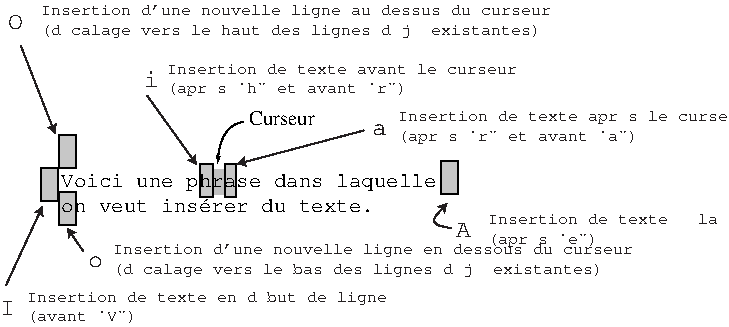
\includegraphics{ann-edt-vi/insert-cmds}
\caption{\label{ann-edt-vi-insert-fig}R{\'e}sum{\'e} des commandes d'insertion
	de texte de "{\tt vi}".}
\end{figure}

\begin{remarque}
Toutes les commandes d'insertion pr{\'e}sent{\'e}es ici, permettent
d'ins{\'e}rer plusieurs lignes. En effet, il suffit de taper son texte
{\it au kilom{\`e}tre} et presser sur la touche {\returnkey} pour
cr{\'e}er une autre ligne, comme tout autre {\'e}diteur de texte
{\it pleine page}. Par contre, vous ne pouvez revenir en arri{\`e}re que sur
la m{\^e}me ligne que le curseur. Si vous d{\'e}sirez revenir sur une
ligne pr{\'e}c{\'e}dente, que vous avez saisi sans sortir du mode
insertion, {\bf il vous faudra revenir en mode commande pour vous y
placer}.
\end{remarque}


%%%%%%%%%%%%%%%%%%%%%%%%%%
\subsection{\label{ann-edt-vi-undo}Annuler ou r{\'e}p{\'e}ter des commandes}

\begin{longtable}{p{4cm}@{\hspace{0.5cm}}p{7cm}}
	\multicolumn{2}{r}{{\sl Suite page suivante $\cdots$}}	\\
\endfoot
\endlastfoot
	{\tt u}		&
		Annule la derni{\`e}re commande.
		\\[2ex]
	{\tt U}		&
		Restaure la ligne courrante {\`a} son {\'e}tat d'origine.
		\\[2ex]
%%	{\tt "}{\sl n}{\tt p}	&
%%		A VOIR
%%		\\[2ex]
%%	{\tt "1pu.uu}	&
%%		A VOIR
%%		\\[2ex]
	{\tt n}		&
		R{\'e}p{\`e}te la derni{\`e}re op{\'e}ration de recherche "{\tt /}" ou "{\tt ?}".
		(cf. section \ref{ann-edt-vi-search}). Cette op{\'e}ration s'effectue de la
		position courrante vers la fin du fichier.
		\\[2ex]
	{\tt N}		&
		R{\'e}p{\`e}te la derni{\`e}re op{\'e}ration de recherche "{\tt /}" ou "{\tt ?}".
		(cf. section \ref{ann-edt-vi-search}). Cette op{\'e}ration s'effectue {\bf
		en sens inverse}, c'est-{\`a}-dire de la position courrante vers {\bf le
		d{\'e}but du fichier}.
		\\[2ex]
	{\tt ;}		&
		R{\'e}p{\`e}te la derni{\`e}re commande de recherche "{\tt f}", "{\tt F}",
		"{\tt t}" ou "{\tt T}" (cf. section \ref{ann-edt-vi-searchop}).
		\\[2ex]
	{\tt ,}		&
		R{\'e}p{\`e}te la derni{\`e}re commande de recherche "{\tt f}", "{\tt F}",
		"{\tt t}" ou "{\tt T}" {\bf en sens inverse}(cf. section
		\ref{ann-edt-vi-searchop}).
		\\[2ex]
	{\tt .}		&
		R{\'e}p{\`e}te la derni{\`e}re op{\'e}ration de insertion/suppression ou modification
		de texte dans le fichier.
		\\[2ex]
\end{longtable}


%%%%%%%%%%%%%%%%%%%%%%%%%%
\subsection{\label{ann-edt-vi-move}D{\'e}placement du curseur}

\begin{longtable}{p{3cm}@{\hspace{0.5cm}}p{8cm}}
	\multicolumn{2}{r}{{\sl Suite page suivante $\cdots$}}	\\
\endfoot
\endlastfoot
	{\tt k} ou \control{p}					&
		D{\'e}placement vers le haut.		\\
	ou \key{$\uparrow$}						&
		\\[2ex]
	{\tt j} ou \control{j} 					&
		D{\'e}placement vers le bas.		\\
	ou \control{n} ou \key{$\downarrow$}	&
		\\[2ex]
	{\tt h} ou \control{h}					&
		D{\'e}placement vers la gauche			\\
	ou \key{{\small \sc Back Space}} ou \key{$\leftarrow$}	&
		\\[2ex]
	{\tt l} ou {\spacekey} ou \key{$\rightarrow$}	&
		D{\'e}placement vers la droite.
		\\[2ex]
	{\tt w} ou {\tt W}	&
		D{\'e}place le curseur au d{\'e}but du mot suivant. "{\tt W}" permet d'ignorer la
		ponctuation.
		\\[2ex]
	{\tt b} ou {\tt B}	&
		D{\'e}place le curseur au d{\'e}but du mot pr{\'e}c{\'e}dent. "{\tt B}" permet d'ignorer la
		ponctuation.
		\\[2ex]
	{\tt e} ou {\tt E}	&
		D{\'e}place le curseur {\`a} la fin du mot courrant. "{\tt E}" permet d'ignorer la
		ponctuation.
		\\[2ex]
	{\tt 0} (z{\'e}ro) ou {\tt |} (pipe)	&
		D{\'e}place le curseur {\`a} la premi{\`e}re colonne de la ligne courrante.
		\\[2ex]
	{\sl n}{\tt |} (pipe)	&
		D{\'e}place le curseur {\`a} la colonne "{\sl n}" de la ligne courrante.
		\\[2ex]
	\verb=^=	&
		D{\'e}place le curseur sur le premier caract{\`e}re diff{\'e}rent de l'espace ou de
		la tabulation sur la ligne courrante.
		\\[2ex]
	\verb=$=	&
		D{\'e}place le curseur {\`a} la fin de la ligne courrante.
		\\[2ex]
	{\tt +} ou {\returnkey}	&
		Deplace le curseur au d{\'e}but de la ligne suivante.
		\\[2ex]
	{\tt -}	&
		D{\'e}place le curseur sur le premier caract{\`e}re diff{\'e}rent de l'espace ou de la
		tabulation de la ligne pr{\'e}c{\'e}dente.
		\\[2ex]
	{\tt 1G}	&
		Ram{\`e}ne le cuseur {\`a} la premi{\`e}re ligne.
		\\[2ex]
	{\tt G}	&
		D{\'e}place le curseur {\`a} la fin du fichier.
		\\[2ex]
	\verb=G$=	&
		D{\'e}place le curseur {\`a} la fin de la derni{\`e}re ligne du fichier.
		\\[2ex]
	{\sl n}{\tt G}	&
		D{\'e}place le curseur {\`a} la $n^e$ ligne du fichier.
		\\[2ex]
	{\tt (}	&
		Ram{\`e}ne le curseur au d{\'e}but de la phrase courrante. Une phrase, pour "{\tt vi}"
		est une suite de mots s{\'e}par{\'e}s par des espaces ou des caract{\`e}res de ponctuations
		et termin{\'e}s par le caract{\`e}re "{\tt .}".
		\\[2ex]
	{\tt )}	&
		D{\'e}place le curseur au d{\'e}but de la phrase suivante.
		\\[2ex]
	\verb={=	&
		Ram{\`e}ne le curseur au d{\'e}but du paragraphe courrant. Un paragraphe, pour
		"{\tt vi}", est une suite de phrases s{\'e}par{\'e}s par une ligne blanche. Cette
		terminologie ob{\'e}it {\`a} la syntaxe de {\TeX} et de {\LaTeX}.
		\\[2ex]
	\verb=}=	&
		D{\'e}place le curseur au d{\'e}but du paragraphe pr{\'e}c{\'e}dent.
		\\[2ex]
\end{longtable}

La figure \ref{ann-edt-vi-movefig} d{\'e}crit les diff{\'e}rentes actions de ces commandes
en fonction de la position du curseur dans le fichier.

\begin{figure}[hbtp]
%\epsfbox{_Images/ann-edt-vi/move-cmds.eps}
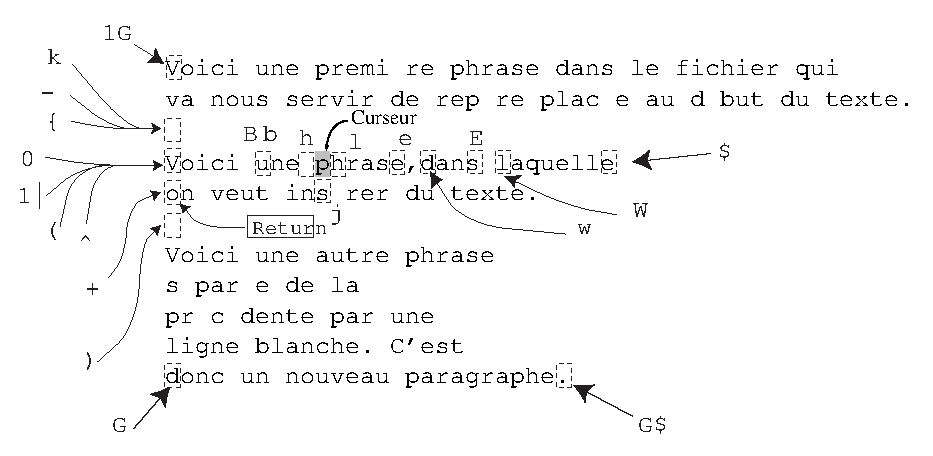
\includegraphics{ann-edt-vi/move-cmds}
\caption{\label{ann-edt-vi-movefig}Commandes de d{\'e}placement du curseur avec
"{\tt vi}".}
\end{figure}

Sachant que "{\tt vi}" a {\'e}t{\'e} d{\'e}di{\'e} aux d{\'e}veloppeurs {\Unix}, il est
clair que "{\tt vi}" reprend des notions du langage C. Lorsque la
premi{\`e}re colonne d'une ligne du fichier contient le caract{\`e}re
"\verb={=", "{\tt vi}" consid{\`e}re tout le texte compris entre ces
deux marques (texte compris entre deux "\verb={=" situ{\'e}s en premi{\`e}re
colonne) comme une section. Par exemple~:\\[2ex]
\begin{quote}
\begin{verbatim}
{
    Le caractere sur la ligne precedente permet de marquer une section.
    La prochaine section commencera des que le caractere { apparaitra
    a nouveau en premiere colonne dans le fichier.
{
    Ici nous sommes dans une nouvelle section. On pourrait faire l'analogie
    avec le langage C lorsque l'on declare le corps d'une
    fonction. En effet on aura :
main()
{
    section associee au corps de la fonction main.
    Donc nous sommes ici dans la troisieme section de ce fichier texte.
}

ma_fonction()
{
    section associee au corps de la fonction ma_fonction.
    Donc nous sommes ici dans la quatrieme section de ce fichier texte.
}
\end{verbatim}
\end{quote}

Pour se d{\'e}placer d'une section {\`a} l'autre, "{\tt vi}" dispose des commandes
suivantes~:

\begin{longtable}{p{4cm}@{\hspace{0.5cm}}p{7cm}}
	\multicolumn{2}{r}{{\sl Suite page suivante $\cdots$}}	\\
\endfoot
\endlastfoot
	\verb=[[=	&
		Ram{\`e}ne le curseur au d{\'e}but de la section courrante.
		\\[2ex]
	\verb=]]=	&
		D{\'e}place le curseur au d{\'e}but de la section suivante.
		\\[2ex]
\end{longtable}


%%%%%%%%%%%%%%%%%%%%%%%%%%
\subsection{\label{ann-edt-vi-del}Effacement de texte}

Dans toute la suite de cette section, le caract{\`e}re courrant d{\'e}signera
celui sur lequel est positionn{\'e} le curseur. De m{\^e}me, la ligne courrant
sera celle ou se trouve le curseur.

Pour "{\tt vi}", un mot est une s{\'e}quence de caract{\`e}res alphanum{\'e}riques
s{\'e}par{\'e}s par un ou plusieurs espaces ou tabulation ou bien encore un
caract{\`e}re de ponctuation. Le mot courrant d{\'e}signe la chaine de caract{\`e}re
{\bf commen\c{c}ant {\`a} la position du curseur} jusqu'{\`a} un caract{\`e}re valide de 
d{\'e}limitatio pour un mot.

\begin{longtable}{p{4cm}@{\hspace{0.5cm}}p{7cm}}
	\multicolumn{2}{r}{{\sl Suite page suivante $\cdots$}}	\\
\endfoot
\endlastfoot
	\control{h} ou \key{{\small \sc Back Space}}	&
		{\bf En mode insertion}, efface le caract{\`e}re pr{\'e}c{\'e}dent.
		\\[2ex]
	\control{w}	&
		{\bf En mode insertion}, efface le mot pr{\'e}c{\'e}dent.
		\\[2ex]
	\control{x}	&
		{\bf En mode \sl insertion}, efface tout le texte ins{\'e}r{\'e} depuis le d{\'e}but
		du mode "{\sl insertion}".
		\\[2ex]
	{\sl n}{\tt x}	&
		Efface les "{\sl n}" caract{\`e}res suivants y compris le caract{\`e}re
		courrant. Si "{\sl n}" n'est pas sp{\'e}cifi{\'e}, "{\tt vi}" n'efface
		que le caract{\`e}re courrant.
		\\[2ex]
	{\sl n}{\tt X}	&
		Efface les "{\sl n}" caract{\`e}res pr{\'e}c{\'e}dents y compris le caract{\`e}re
		courrant. Si "{\sl n}" n'est pas sp{\'e}cifi{\'e}, "{\tt vi}" n'efface
		que le caract{\`e}re pr{\'e}c{\'e}dent.
		\\[2ex]
	{\tt xp}	&
		Intervertit le caract{\`e}re courrant avec le caract{\`e}re suivant.
		\\[2ex]
	{\sl n}{\tt dw}	&
		Efface les "{\sl n}" mots suivants. Si "{\sl n}" n'est pas
		sp{\'e}cifi{\'e}, "{\tt vi}~�> d{\'e}truit le mot courrant. Pour rappel, un
		mot est une suite de caract{\`e}res s{\'e}par{\'e}s par un ou plusieurs espaces
		ou tabulation ou bien par un caract{\`e}re de ponctuation.
		\\[2ex]
	{\sl n}{\tt db}	&
		Efface les "{\sl n}" mots pr{\'e}c{\'e}dents. Si "{\sl n}" n'est pas
		sp{\'e}cifi{\'e}, "{\tt vi}~�> d{\'e}truit le mot courrant.
		\\[2ex]
	{\sl n}{\tt dd}	&
		Efface les "{\sl n}" lignes suivantes en commen\c{c}ant par la
		ligne courrante. Si <<n {\sl n}" n'est pas sp{\'e}cifi{\'e}, "{\tt vi}"
		ne d{\'e}truit que la ligne courrante.
		\\[2ex]
	{\tt :}{\sl n,m}{\tt d}	&
		D{\'e}truit les lignes de "{\sl n}" {\`a} "{\sl m}". Si 
		"$n \in \mathcal{N}$" ou "$m \in \mathcal{N}$", alors
		l'op{\'e}ration de destruction commence ou se termine {\`a} la ligne dont
		le num{\'e}ro est sp{\'e}cifi{\'e}. Si "{\sl n}" ou "{\sl m}" est un
		marqueur, l'op{\'e}ration de destruction commence ou se termine
		{\`a} la position indiqu{\'e}e par le marqueur (cf. section
		\ref{ann-edt-vi-intro}). Si "{\sl n}" ou "{\sl m}" est une
		expression r{\'e}guli{\`e}re d{\'e}limit{\'e}e par le caract{\`e}re "{\tt /}",
		l'op{\'e}ration commence {\`a} la premi{\`e}re ligne trouv{\'e}e {\`a} partir
		de la position courrant satisfaisant
		l'expression r{\'e}guli{\`e}re ou bien se termine {\`a} la {\bf premi{\`e}re}
		ligne  satisfaisant l'expression r{\'e}guli{\`e}re se trouvant
		{\`a} la suite de la premi{\`e}re ligne {\`a} effacer. 
		\\[2ex]
	{\tt D}	ou \verb=d$=	&
		D{\'e}truit tout ce qui suit {\`a} partir de la position courrante du
		curseur jusqu'{\`a} la fin de la ligne.
		\\[2ex]
	{\tt d}{\sl cmd$_{curseur}$}	&
		D{\'e}truit le texte {\`a} partir de la position courrante du curseur
		jusqu'au point indiqu{\'e} par la commande de d{\'e}placement du
		cuseur "{\sl cmd$_{curseur}$}". Par exemple, "{\tt dG}"
		efface toutes les lignes {\`a} partir de la position courrante jusqu'{\`a}
		la fin de fichier. Cet exemple est {\'e}quivalent {\`a} "\verb=:.,$d=".
		Reportez-vous {\`a} la section \ref{ann-edt-vi-move} pour les
		commandes de d{\'e}placement du curseur.		
		\\[2ex]
\end{longtable}

La figure \ref{ann-edt-vi-delfig} d{\'e}crit les diff{\'e}rentes actions de ces commandes
en fonction de la position du curseur dans le fichier.

\begin{figure}[hbtp]
%\epsfbox{_Images/ann-edt-vi/delete-cmds.eps}
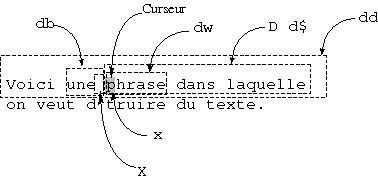
\includegraphics{ann-edt-vi/delete-cmds}
\caption{\label{ann-edt-vi-delfig}Commandes de suppression de texte avec
"{\tt vi}".}
\end{figure}

%%%%%%%%%%%%%%%%%%%%%%%%%%
\subsection{\label{ann-edt-vi-search}Recherche}

%%%%%%%%%%%%%%
\subsubsection{\label{ann-edt-vi-searchcmds}Expression de recherches}

\begin{longtable}{p{4cm}@{\hspace{0.5cm}}p{7cm}}
	\multicolumn{2}{r}{{\sl Suite page suivante $\cdots$}}	\\
\endfoot
\endlastfoot
	\verb*=:set magic=		&
		Autorise les expressions de recherche en utilisant les expressions
		r{\'e}guli{\`e}res (cf. chapitre \ref{reg-exp}). Cette option est positionn{\'e}e
		par d{\'e}faut (cf. section \ref{ann-edt-vi-config}).
		\\[2ex]
	\verb*=:set nomagic=	&
		N'autorise que les symboles "\verb=^=" et "\verb=$=" pour
		les expressions de recherche. Pour plus de pr{\'e}cisions sur les
		options de "{\tt vi}", reportez-vous {\`a} la section \ref{ann-edt-vi-config}.
		\\[2ex]
	\verb=^=				&
		Correspond au d{\'e}but de ligne (idem que les expressions r{\'e}guli{\`e}res,
		cf. \ref{reg-exp}).
		\\[2ex]
	\verb=$=				&
		Correspond {\`a} la fin de ligne (idem que les expressions r{\'e}guli{\`e}res,
		cf. \ref{reg-exp}).
		\\[2ex]
	\verb=.=				&
		Correspond {\`a} n'importe quel caract{\`e}re (idem que les expressions r{\'e}guli{\`e}res,
		cf. \ref{reg-exp}).
		\\[2ex]
	\verb=\<=				&
		Correspond {\`a} un d{\'e}but de mot.
		\\[2ex]
	\verb=\>=				&
		Correspond {\`a} une fin de mot.
		\\[2ex]
	\verb=[={\sl str}\verb=]=	&
		Correspond {\`a} un et un seul caract{\`e}re parmi ceux composant
		"{\sl str}" (idem que les expressions r{\'e}guli{\`e}res,
		cf. \ref{reg-exp}).
		\\[2ex]
	\verb=[^={\sl str}\verb=]=	&
		Correspond {\`a} un et un seul caract{\`e}re diff{\'e}rent de ceux
		composant "{\sl str}" (idem que les expressions r{\'e}guli{\`e}res,
		cf. \ref{reg-exp}).
		\\[2ex]
	\verb=[={\sl a-w}\verb=]=	&
		Correspond {\`a} un et un seul caract{\`e}re entre les caract{\`e}res
		"{\sl a}" et "{\sl w}" (idem que les expressions r{\'e}guli{\`e}res,
		cf. \ref{reg-exp}).
		\\[2ex]
	\verb=*=				&
		Sp{\'e}cifie le nombre d'occurence qu'un caract{\`e}re peut appara{\^\i}tre. Dans
		ce cas, le caract{\`e}re sp{\'e}cifi{\'e} peut appara{\^\i}tre un nombre quelconque
		de fois ( $n \in \{0, \cdots, +\infty\}$).
		\\[2ex]
	\verb=\=				&
		Annule l'interpr{\'e}tation du caract{\`e}re suivant.
		\\[2ex]
	\verb=\\=				&
		Permet de sp{\'e}cifier le caract{\`e}re "\verb=\=". En effet,
		"\verb=\\=" implique que~:
			\begin{itemize}
				\item	le premier "\verb=\=" annule l'{\'e}valuation
						du caract{\`e}re suivant.
				\item	le second caract{\`e}re "\verb=\=" doit {\^e}tre pris
						tel quel.
			\end{itemize}
		\\[2ex]
\end{longtable}

\begin{remarque}
Ce tableau montre que les r{\`e}gles de syntaxes des expressions r{\'e}guli{\`e}res
sont largement utilis{\'e}es dans "{\tt vi}". Tout comme les commandes
"{\tt sed}" et "{\tt awk}" (cf. chapitres \ref{adv-fltrs-sed} et
\ref{adv-fltrs-awk}), "{\tt vi}" fait partie des nombreuses commandes
{\Unix} utilisant la notion des expressions r{\'e}guli{\`e}res.
\end{remarque}

%%%%%%%%%%%%%%
\subsubsection{\label{ann-edt-vi-searchop}Op{\'e}rations de recherche}

\begin{longtable}{p{4cm}@{\hspace{0.5cm}}p{7cm}}
	\multicolumn{2}{r}{{\sl Suite page suivante $\cdots$}}	\\
\endfoot
\endlastfoot
	\verb=%=						&
		Permet de localiser la parenth{\`e}se fermante ou ouvrante correspondant
		{\`a} celle sur laquelle est positionn{\'e} le curseur. Cette fonctionnalit{\'e}
		est op{\'e}rationnelle pour "\verb=(=,\verb=)=", "\verb=[=,\verb=]="
		et "\verb={=,\verb=}=".
		\\[2ex]
	{\tt f}{\sl caract}				&
		Recherche, dans la ligne courrante, le premier caract{\`e}re
		"{\sl caract}", {\bf suivant} la position courrante du curseur.
		\\[2ex]
	{\tt F}{\sl caract}				&
		Recherche, dans la ligne courrante, le premier caract{\`e}re
		"{\sl caract}", {\bf pr{\'e}c{\'e}dant} la position courrante du curseur.
		\\[2ex]
	{\tt t}{\sl caract}				&
		Recherche, dans la ligne courrante, le premier caract{\`e}re
		imm{\'e}diatement pr{\'e}c{\'e}dent {\`a} "{\sl caract}", {\bf suivant} la
		position courrante du curseur.
		\\[2ex]
	{\tt T}{\sl caract}				&
		Recherche, dans la ligne courrante, le premier caract{\`e}re
		imm{\'e}diatement suivant {\`a} "{\sl caract}", {\bf pr{\'e}c{\'e}dant} la
		position courrante du curseur.
		\\[2ex]
	{\tt /}{\sl str}{\returnkey}	&
		Recherche la chaine "{\sl str}" de la position courrante
		du curseur vers la {\bf fin} du fichier.
		\\[2ex]
	{\tt ?}{\sl str}{\returnkey}	&
		Recherche la chaine "{\sl str}" de la position courrante
		du curseur vers le {\bf d{\'e}but} du fichier.
		\\[2ex]
	\verb*=:set ic=					&
		Ignore la diff{\'e}rence entre les majuscules et les minuscules.
		Pour plus d'informations sur les options de "{\tt vi}",
		reportez-vous {\`a} la section \ref{ann-edt-vi-config}.
		\\[2ex]
	\verb*=:set noic=				&
		Fait la diff{\'e}rence entre les majuscules et les minuscules.
		C'est le comportement par d{\'e}faut. Pour plus d'informations
		sur les options de "{\tt vi}", reportez-vous {\`a} la section
		\ref{ann-edt-vi-config}.
		\\[2ex]
\end{longtable}

%%%%%%%%%%%%%%
\subsubsection{\label{ann-edt-vi-searchglob}Recherche globale et substitution}

\begin{longtable}{p{3.5cm}@{\hspace{0.5cm}}p{7.5cm}}
	\multicolumn{2}{r}{{\sl Suite page suivante $\cdots$}}	\\
\endfoot
\endlastfoot
	{\tt :{\sl n,m}s/{\sl str$_1$}/{\sl str$_2$}/{\sl opt}}		&
		Substitue l'expression "{\sl str$_1$}" par "{\sl str$_2$}"
		dans l'espace de travail d{\'e}limit{\'e} par "{\sl n}" et
		"{\sl m}", c'est-{\`a}-dire sur toutes les lignes du fichier
		caract{\'e}ris{\'e}es par "{\sl n}" et "{\sl m}". Les options
		disponibles sont~:
		\begin{description}
			\item[{\rm "{\tt g}"~:}]
				La substitution est globale, c'est-{\`a}-dire qu'elle se
				r{\'e}p{\`e}te autant de fois que n{\'e}cessaire sur chaque ligne
				s{\'e}lectionn{\'e}e. Par d{\'e}faut, la substitution ne s'effectue
				qu'{\bf une seule fois} par ligne.
			\item[{\rm "{\tt c}"~:}]
				Une confirmation est demand{\'e}e avant d'{\'e}ffectuer toute op{\'e}ration
				de substitution. Il suffit d'appuyer sur \key{y} pour
				confirmer et sur {\returnkey} ou \key{n} pour infirmer.
			\item[{\rm "{\tt p}"~:}]
				Les lignes modifi{\'e}es sont affich{\'e}es.
		\end{description}
		Cette commande est identique {\`a} la commande "{\tt s}" de
		"{\tt sed}" (cf. \ref{sed-cmds}).
		\\[2ex]
	\verb*=&=		&
		R{\'e}p{\`e}te l'appel {\`a} la derni{\`e}re commande de substitution "{\tt :s}".
		\\[2ex]
	{\tt :g/{\sl str}/{\sl cmd}}		&
		Ex{\'e}cute la commande "{\sl cmd}" sur toutes les lignes contenant
		l'expression "{\tt str}".
		\\[2ex]
	{\tt :g/{\sl str$_1$}/s/{\sl str$_2$}/{\sl str$_3$/}}	&
		Localise la ligne contenant l'expression "{\sl str$_1$}" et
		y substitue "{\sl str$_2$}" par "{\sl str$_3$/}".
		\\[2ex]
	{\tt :v/{\sl str}/{\sl cmd}}	&
		Ex{\'e}cute la commande "{\sl cmd}" sur toutes les lignes {\bf ne
		contenant pas} l'expression "{\sl str}".
		\\[2ex]
\end{longtable}

%%%%%%%%%%%%%%%%%%%%%%%%%%
\subsection{\label{ann-edt-vi-indent}Indentation de texte}

\begin{longtable}{p{4cm}@{\hspace{0.5cm}}p{7cm}}
	\multicolumn{2}{r}{{\sl Suite page suivante $\cdots$}}	\\
\endfoot
\endlastfoot
	\control{i} ou {\tabkey}									&
		En mode "{\sl insertion}", ins{\`e}re un caract{\`e}re de tabulation
		servant {\`a} l'indentation du programme.
		\\[2ex]
	\verb*,:set ai,												&
		Active ou d{\'e}asctive l'indentation automatique (cf. section
		\ref{ann-edt-vi-config}). Si l'indentation automatique est
		activ{\'e}e, lorsque vous tapez un retour chariot, "{\tt vi}"
		ins{\`e}re automatiquement le nombre n{\'e}cessaire de tabulations afin
		que la nouvelle ligne commence au m{\^e}me niveau que la ligne pr{\'e}c{\'e}dente.
		\\[2ex]
	\verb*,:set sw=,{\sl n}										&
		Fixe, {\bf pour l'affichage}, la taille d'une tabulation. {\bf Attention},
		cette commande ne modifie pas le contenu du fichier en rempla\c{c}ant
		les tabulations par un certain nombre d'espaces, les caract{\`e}res
		de tabulation (code {\ASCII} 9) sont bien pr{\'e}sents dans le fichier.
		"{\tt vi}" interpr{\`e}tera ces caract{\`e}res pour les faire
		correspondre {\`a} une certaine taille, c'est-{\`a}-dire {\`a} un certain nombre
		de colonnes. Par cons{\'e}quent, si vous modifiez la taille des tabulations
		(par d{\'e}faut toutes les 8 colonnes), d'autres {\'e}diteurs pourront
		donner un pr{\'e}sentation diff{\'e}rent de votre code source, {\`a} moins
		biens{\^u}r d'y modifier aussi la taille des taille des tabulations.
		\\[2ex]
	{\sl n}\verb=<<= ou {\sl n}\verb=>>=							&
		D{\'e}cale vers la gauche ("\verb=<<=") ou vers la droite
		("\verb=>>=") les <<{\sl n}" lignes. Si "{\sl n}"
		n'est pas pr{\'e}cis{\'e}, "{\tt vi}" d{\'e}cale la ligne courrante.
		\\[2ex]
	\verb=<={\sl cmd$_{curseur}$} ou \verb=>={\sl cmd$_{curseur}$}	&
		Permet de d{\'e}caler plusieurs lignes vers la gauche ("\verb=<=")
		ou vers la droite ("\verb=>=") en fonction de la commande de
		d{\'e}placement du curseur "{\sl cmd$_{curseur}$}" (cf. section
		\ref{ann-edt-vi-move}).
		\\[2ex]
\end{longtable}

%%%%%%%%%%%%%%%%%%%%%%%%%%
\subsection{\label{ann-edt-vi-cutpaste}Copier/Coller}

"{\tt vi}" dispose d'un certain nombre de {\sl buffer} permettant
de copier ou coller un certain nombre de lignes, de mots ou de caract{\`e}res
qu'il sera possible de replacer n'importe o{\`u} dans le fichier.Ces
{\sl buffers} sont nomm{\'e}s par une lettre allant de "{\tt a}" {\`a}
"{\tt z}".

Dans toute la suite, nous d{\'e}signerons l'op{\'e}ration "{\sl couper}"
par le fait de copier du texte dans un {\sl buffer} et de les
effacer du fichier. De m{\^e}me, nous d{\'e}signerons l'op{\'e}ration "{\sl coller}"
par le fait de placer {\`a} la position courrante du curseur, le contenu
d'un {\sl buffer}.

Dans le tableau suivant, nous d{\'e}signerons l'un de ces {\sl buffers}
par "{\sl (a-z)}".

\begin{longtable}{p{2.5cm}@{\hspace{0.5cm}}p{8.5cm}}
	\multicolumn{2}{r}{{\sl Suite page suivante $\cdots$}}	\\
\endfoot
\endlastfoot
	{\sl n}{\tt yy} ou {\sl n}{\tt Y}	&
		Copie les "{\sl n}" lignes {\`a} partir de la position
		courrante dans le {\sl buffer} par d{\'e}faut. Si "{\sl n}" n'est
		pas pr{\'e}cis{\'e}, alors seule la ligne courrante est m{\'e}moris{\'e}e
		dans le {\sl buffer}.
		\\[2ex]
	{\tt y}{\sl cmd$_{curseur}$}		&
		Copie la partie de texte sp{\'e}cifi{\'e}e par la commande
		de d{\'e}placement de curseur "{\sl cmd$_{curseur}$}" dans
		le {\sl buffer} par d{\'e}faut, {\`a} partir de la position du curseur.
		Par exemple, "{\tt yG}", copie le texte {\`a} partir de la
		position courrante du curseur jusqu'{\`a} la fin de la ligne dans le
		{\sl buffer}.
		\\[2ex]
	{\tt "{\sl (a-z)n}yy}				&
		Copie les "{\sl n}" lignes {\`a} partir de la position
		courrante dans le {\sl buffer} sp{\'e}cifi{\'e}. Si "{\sl n}" n'est pas
		pr{\'e}cis{\'e}, alors seule la ligne courrante est m{\'e}moris{\'e}e
		dans le {\sl buffer}. Par exemple, "{\tt "a10yy}" copie
		les dix lignes suivantes (ligne courrante comprise) dans
		le {\sl buffer} "{\tt a}".
		\\[2ex]
	{\tt "{\sl (a-z)n}dd}				&
		{\sl Coupe} les "{\sl n}" lignes {\`a} partir de la position
		courrante dans le {\sl buffer} sp{\'e}cifi{\'e}. Si "{\sl n}" n'est pas
		pr{\'e}cis{\'e}, alors seule la ligne courrante est m{\'e}moris{\'e}e
		dans le {\sl buffer}. Par exemple, "{\tt "a10dd}" {\sl coupe}
		les dix lignes suivantes (ligne courrante comprise) dans
		le {\sl buffer} "{\tt a}".
		\\[2ex]
	{\tt p} (minuscule)					&
		{\sl Colle} le contenu du {\sl buffer} par d{\'e}faut {\bf apr{\`e}s}�a
		position courrante du curseur. Apr{\`e}s cette op{\'e}ration, le {\sl buffer}
		est vid{\'e}. 
		\\[2ex]
	{\tt P} (majuscule)					&
		{\sl Colle} le contenu du {\sl buffer} par d{\'e}faut {\bf avant}�a
		position courrante du curseur. Apr{\`e}s cette op{\'e}ration, le {\sl buffer}
		est vid{\'e}. 
		\\[2ex]
	{\tt "{\sl (a-z)n}p}�			&
		{\sl Colle} le contenu du {\sl buffer} sp{\'e}cifi{\'e} {\bf apr{\`e}s}�a
		position courrante du curseur. Apr{\`e}s cette op{\'e}ration, le {\sl buffer}
		est vid{\'e}. 
		\\[2ex]
	{\tt "{\sl (a-z)n}P}				&
		{\sl Colle} le contenu du {\sl buffer} sp{\'e}cifi{\'e} {\bf avant}�a
		position courrante du curseur. Apr{\`e}s cette op{\'e}ration, le {\sl buffer}
		est vid{\'e}. 
		\\[2ex]
\end{longtable}

%%%%%%%%%%%%%%%%%%%%%%%%%%
\subsection{\label{ann-edt-vi-mod}Modifier du texte}

\begin{longtable}{p{4cm}@{\hspace{0.5cm}}p{7cm}}
	\multicolumn{2}{r}{{\sl Suite page suivante $\cdots$}}	\\
\endfoot
\endlastfoot
	{\tt r{\sl caract}}						&
		Substitue le caract{\`e}re courrant par le caract{\`e}re "{\sl caract}".
		\\[2ex]
	{\tt R{\sl texte}{\esckey}}				&
		R{\'e}{\'e}crit le texte saisi "{\sl texte}" par dessus ce qui est
		d{\'e}j{\`a} pr{\'e}sent. Ceci {\'e}quivaut au mode "{\sl surimpression}"
		des {\'e}diteurs pleine-page classiques comme "{\tt EVE}" ou
		"{\tt LSEDIT}" sous {\OpenVMS}. Le remplacement de texte
		se termine par la touche {\esckey}. En mode "{\sl insertion}",
		le texte saisi est ins{\'e}r{\'e} {\`a} la position courrante du curseur.
		En mode "{\sl surimpression}", tout ce qui est saisi vient
		s'{\'e}crire par dessus le texte d{\'e}j{\`a} existant.
		\\[2ex]
	{\tt s{\sl texte}{\esckey}}				&
		Substitue le caract{\`e}re courrant avec le texte saisi "{\sl texte}".
		L'insertion du nouveau texte se termine par {\esckey}. Par cons{\'e}quent,
		apr{\`e}s la saisie de la commande "{\tt s}", "{\tt vi}" passe
		en mode "{\sl insertion}".
		\\[2ex]
	{\tt S{\sl texte}{\esckey}} ou {\tt cc{\sl texte}{\esckey}}	&
		Efface la ligne courrante et la substitue par le texte saisi
		"{\sl texte}". L'insertion du nouveau texte se termine par
		{\esckey}. Par cons{\'e}quent, apr{\`e}s la saisie de la commande
		"{\tt s}" ou "{\tt cc}", "{\tt vi}" passe
		en mode "{\sl insertion}".
		\\[2ex]
	{\tt cw{\sl texte}{\esckey}}			&
		Change le mot courrant par le texte saisi "{\sl texte}".
		L'insertion du nouveau texte se termine par {\esckey}. Par cons{\'e}quent,
		apr{\`e}s la saisie de la commande "{\tt cw}", "{\tt vi}" passe
		en mode "{\sl insertion}".
		\\[2ex]
	{\tt C{\sl texte}{\esckey}}				&
		Change le reste de la ligne {\`a} partir de la position courrante par le
		texte saisi "{\sl texte}". L'insertion du nouveau texte se termine
		par {\esckey}. Par cons{\'e}quent, apr{\`e}s la saisie de la commande
		"{\tt C}", "{\tt vi}" passe en mode "{\sl insertion}".
		\\[2ex]
	{\tt c{\sl curs$_{cmd}$texte}{\esckey}}	&
		De fa\c{c}on plus g{\'e}n{\'e}rale, la commande "{\tt c}" suivie d'une
		commande "{\tt vi}" de d{\'e}placement de curseur (cf. section
		\ref{ann-edt-vi-move}), change le texte correspondant avec ce qui a
		{\'e}t{\'e} saisi, jusqu'{\`a} ce que la touche {\esckey} soit press{\'e}e.
		Par cons{\'e}quent, apr{\`e}s la saisie de la commande
		"{\tt c{\sl curs$_{cmd}$}}", "{\tt vi}" passe en mode
		"{\sl insertion}".
		\\[2ex]	
	{\tt J}									&
		Rassemble la ligne courrante et la ligne suivante sur une seule et
		m{\^e}me ligne.
		\\[2ex]
	{\tt {\sl n}J}							&
		Rassemble les "{\sl n}" lignes, y compris la ligne courrante, sur
		une seule et m{\^e}me ligne.
		\\[2ex]
\end{longtable}

%%%%%%%%%%%%%%%%%%%%%%%%%%
\subsection{\label{ann-edt-vi-place}Placement direct du curseur et ajustement
			du texte {\`a} l'{\'e}cran}

\begin{longtable}{p{4cm}@{\hspace{0.5cm}}p{7cm}}
	\multicolumn{2}{r}{{\sl Suite page suivante $\cdots$}}	\\
\endfoot
\endlastfoot
	{\tt H}									&
		Ram{\`e}ne le curseur sur la premi{\`e}re ligne de l'{\'e}cran, ligne qui n'est
		pas forc{\'e}ment la premi{\`e}re ligne du fichier.
		\\[2ex]
	{\tt {\sl n}H}							&
		Ram{\`e}ne le curseur sur la $n^{e}$ ligne de l'{\'e}cran, ligne qui n'est pas
		forc{\'e}ment la $n^{e}$ ligne du fichier.
		\\[2ex]
	{\tt M}									&
		Am{\`e}ne le curseur au milieu de l'{\'e}cran.
		\\[2ex]
	{\tt L}									&
		Am{\`e}ne le curseur sur la derni{\`e}re ligne de l'{\'e}cran, ligne qui n'est pas
		forc{\'e}ment la derni{\`e}re ligne du fichier.
		\\[2ex]
	{\tt {\sl n}L}							&
		Am{\`e}ne le curseur sur la $n^{e}$ ligne de l'{\'e}cran en partant du bas de
		l'{\'e}cran.
		\\[2ex]
	\control{e}								&
		D{\'e}cale l'affichage d'une ligne vers le haut.
		\\[2ex]
	\control{y}								&
		D{\'e}cale l'affichage d'une ligne vers le bas.
		\\[2ex]
	\control{u}								&
		D{\'e}cale l'affichage d'une demi page vers le haut.
		\\[2ex]
	\control{d}								&
		D{\'e}cale l'affichage d'une demi page vers le bas.
		\\[2ex]
	\control{b}								&
		D{\'e}cale l'affichage d'une demi page vers le haut. Cette fonction est aussi
		disponible avec la touche "{\sl Page Pr{\'e}c{\'e}dente}".
		\\[2ex]
	\control{f}								&
		D{\'e}cale l'affichage d'une page vers le bas. Cette fonction est aussi
		disponible avec la touche "{\sl Page Suivante}".
		\\[2ex]
	\control{l} (lettre "{\tt l}")		&
		Rafra{\^\i}chit l'{\'e}cran. Cette fonction {\'e}quivaut {\`a} \control{w} avec les
		{\'e}diteurs <<{\tt EVE}" ou "{\tt LSEDIT}" sous {\OpenVMS}.
		\\[2ex]
	{\tt z{\returnkey}}						&
		D{\'e}cale l'affichage de telle sorte que la ligne courrant devienne la
		premi{\`e}re ligne affich{\'e}e en haut de l'{\'e}cran.
		\\[2ex]
	{\tt {\sl n}z{\returnkey}}				&
		D{\'e}cale l'affichage de telle sorte que la $n^{e}$ ligne affich{\'e}e en partant
		du haut, devienne la premi{\`e}re ligne affich{\'e}e {\`a} l'{\'e}cran.
		\\[2ex]
	{\tt z.}								&
		D{\'e}cale l'affiche de telle sorte que la ligne courrante devienne celle
		du milieu de l'{\'e}cran.
		\\[2ex]
	{\tt {\sl n}z.}							&
		D{\'e}cale l'affichage de telle sorte que la $n^{e}$ ligne affich{\'e}e en partant
		du haut, devienne celle du milieur de l'{\'e}cran.
		\\[2ex]
	{\tt z-}								&
		D{\'e}cale l'affichage de telle sorte que la ligne courrante devienne
		la derni{\`e}re ligne affich{\'e}e en bas de l'{\'e}cran.
		\\[2ex]
	{\tt {\sl n}z-}							&
		D{\'e}cale l'affichage de telle sorte que la $n^{e}$ ligne affich{\'e}e en partant
		du haut, devienne la derni{\`e}re ligne affich{\'e}e en bas de l'{\'e}cran.
		\\[2ex]
\end{longtable}

\begin{remarque}
L'ensemble de ces commandes s'adaptent en fonction de la taille de l'{\'e}cran,
c'est-{\`a}-dire du nombre de lignes et de colonnes.
\end{remarque}


%%%%%%%%%%%%%%%%%%%%%%%%%%
\subsection{\label{ann-edt-vi-sh}Interaction avec le {\sl shell}}

\begin{longtable}{p{4cm}@{\hspace{0.5cm}}p{7cm}}
	\multicolumn{2}{r}{{\sl Suite page suivante $\cdots$}}	\\
\endfoot
\endlastfoot
	\verb*=:!={\sl commande}					&
		Ex{\'e}cute la commande dans un sous processus. Cette commande peut
		{\^e}tre n'importe quelle commande {\sl shell}, y compris un appel
		{\`a} une autre session "{\tt vi}". Lors de la saisie de la commande
		au niveau du {\sl prompt} de "{\tt vi}", il est possible
		d'utiliser les caract{\`e}res sp{\'e}ciaux suivants~:
		\\[2ex]
		&
		\begin{tabular}{l@{\hspace{1ex}}p{5cm}}
			\verb=%=	& correspond au nom du fichier en train d'{\^e}tre
				{\'e}dit{\'e}.\\
			\verb=#=	& correspond au nom du dernier fichier {\'e}dit{\'e}.\\
		\end{tabular}
		\\[2ex]
		&
		L'interpr{\'e}teur de commandes utilis{\'e} par d{\'e}faut est le Bourne Shell
		("\verb=/bin/sh=". Cette valeur peut {\^e}tre modifi{\'e}e gr{\^a}ce {\`a}
		la commande "\verb*,:set shell=,{\sl chemin}" (cf.
		\ref{ann-edt-vi-config}).
		\\[2ex]
	\verb*=:!!=									&
		R{\'e}ex{\'e}cute la derni{\`e}re commande {\sl shell}, c'est-{\`a}-dire la
		derni{\`e}re commande "\verb*=:!={\sl commande}".
		\\[2ex]
	\verb*=:r! ={\sl commande}					&
		Inclut dans le fichier {\`a} la position courrante du curseur
		la sortie standard de la commande "{\sl commande}".
		\\[2ex]
	\verb*=:f ={\sl nouv\_fichier}				&
		Renomme le fichier courrant sous le nouveau nom
		"{\sl nouv\_fichier}". Dans ce cas de figure, le fichier
		{\'e}dit{\'e} change de nom sur le disque mais aussi pour "{\tt vi}".
		Ainsi, toute op{\'e}ration future de sauvegarde se fera sous le
		nouveau nom de fichier.
		\\[2ex]
	\verb*=:w !={\sl commande}					&
		Sauvegarde le fichier courrante et envoie son contenu sur l'entr{\'e}e
		standard de la commande "{\sl commande}".
		\\[2ex]
	\verb*=:cd ={\sl r{\'e}pertoire}			&
		Change le r{\'e}pertoire par d{\'e}faut de "{\tt vi}". Si aucun r{\'e}pertoire
		n'est sp{\'e}cifi{\'e}, le contenu de la variable d'environnement
		"{\tt HOME}" est utilis{\'e}.
		\\[2ex]
	\verb*=:sh=									&
		D{\'e}marre un sous processus de "{\tt vi}" dans lequel sera
		ex{\'e}cut{\'e} un nouvel interpr{\'e}teur de commandes. Pour revenir {\`a}
		"{\tt vi}", il suffit de taper la commande "{\tt exit}"
		ou \control{d}, commande ou s{\'e}quence de touche permettant
		de terminer une session {\sl shell} (cf. \ref{bcpts-login}
		et \ref{test-loop-break}).
		\\[2ex]
	\verb*=:so ={\sl fichier}						&
		Lit et ex{\'e}cute les commandes {\sl shell} pr{\'e}sentes dans le
		fichier "{\sl fichier}".
		\\[2ex]
	\verb*=!={\sl cmd$_{curseur}$\verb*= =commande}	&
		Envoie le texte s{\'e}lectionn{\'e} par la commande de d{\'e}placement
		de curseur "{\sl cmd$_{curseur}$}" {\`a} la commande {\sl shell}
		"{\sl commande}". Le texte correspondant {\`a} la commande
		de d{\'e}placement du curseur est remplac{\'e} par la sortie standard
		de la commande. Par exemple~:
		\\[2ex]
		&
		\begin{tabular}{l@{\hspace{1ex}}p{5cm}}
			\verb*=!w ls -l={\returnkey} 	&
			envoie le mot situ{\'e} au niveau du curseur {\`a} la commande
			"{\tt ls -l}". Le mot en question est remplac{\'e} par
			le r{\'e}sultat de la commande.
			\\[2ex]
			\verb*=!}sort={\returnkey}		&
			S{\'e}lectionne le texte de la position courrante du curseur
			jusqu'{\`a} la fin du paragraphe et le trie gr{\^a}ce {\`a} la commande
			"{\tt sort}". Le texte s{\'e}lectionn{\'e} est remplac{\'e} par le
			r{\'e}sultat du tri.
		\end{tabular}
		\\[2ex]
\end{longtable}

%%%%%%%%%%%%%%%%%%%%%%%%%%
\subsection{\label{ann-edt-vi-macros}Macros et abr{\'e}viations}

\begin{longtable}{p{4cm}@{\hspace{0.5cm}}p{7cm}}
	\multicolumn{2}{r}{{\sl Suite page suivante $\cdots$}}	\\
\endfoot
\endlastfoot
	\verb*=:map ={\sl touche}\verb*= ={\sl s{\'e}quence$_{cmds}$}	&
		Associe la s{\'e}quence de commandes
		"{\sl s{\'e}quence$_{cmds}$}" {\`a} la touche "{\sl touche}".
		Ainsi, d{\`e}s que cette touche est appuy{\'e}e, la s{\'e}quence de commandes
		est ex{\'e}cut{\'e}e.
		\\[2ex]
	\verb*=:map=													&
		Affiche l'ensemble des d{\'e}finitions effectu{\'e}es, c'est-{\`a}-dire
		l'ensemble des "{\sl macros}" de "{\tt vi}" cr{\'e}{\'e}es
		gr{\^a}ce {\`a} la commande pr{\'e}c{\'e}dente.
		\\[2ex]
	\verb*=:unmap ={\sl touche}										&
		D{\'e}truit l'association entre une touche et la s{\'e}quence de
		commandes pr{\'e}c{\'e}demment faite. Cette commande d{\'e}truit donc
		la macro associ{\'e}e {\`a} la touche "{\sl touche}".
		\\[2ex]
	\verb*=:ab ={\sl chaine$_1$}\verb*= ={\sl chaine$_2$}			&
		Permet de d{\'e}finir une abr{\'e}viation. Lorsque "{\sl chaine$_1$}"
		est saisi, "{\tt vi}" la substitue par "{\sl chaine$_2$}".
		\\[2ex]
	\verb*=:ab=														&
		Affiche l'ensemble des abr{\'e}viations d{\'e}finies.
		\\[2ex]
	\verb*=:una ={\sl chaine}										&
		D{\'e}truit l'abr{\'e}viation "{\sl chaine}".
		\\[2ex]
\end{longtable}

La commande "{\tt :map}" permer de d{\'e}finir des s{\'e}quences de commandes
ou "{\sl macros}" "{\tt vi}". En effet, par d{\'e}finition, une
macro, comme en langage C ou n'importe quel logiciel, est une s{\'e}rie de
commandes ou d'actions de base regroup{\'e}es sous un nom et appelable
par l'utilisateur.

Si l'option "{\tt timeout}" est positionn{\'e}e (cf. section
\ref{ann-edt-vi-config}), toute ex{\'e}cution de macros ne peut d{\'e}passer une
seconde. Par cons{\'e}quent, si vous utilisez des macros importantes,
d{\'e}sactivez cette option.

Sachant que les commandes "{\tt vi}" utilisent des caract{\`e}res de
contr{\^o}le en mode commande, il est possible de les ins{\'e}rer dans la
d{\'e}finition des macros gr{\^a}ce {\`a} la s{\'e}quence \control{v} (cf. section
\ref{ann-edt-vi-insert}). De m{\^e}me, le caract{\`e}re "{\tt "}" est utilis{\'e}
dans les commandes "{\tt vi}" (cf. sections \ref{ann-edt-vi-undo}
et \ref{ann-edt-vi-cutpaste}). Par cons{\'e}quent, s'il doit {\^e}tre utilis{\'e}
dans une macro dans un autre cadre que celui d'une commande le r{\'e}f{\'e}ren\c{c}ant,
il doit {\^e}tre pr{\'e}c{\'e}d{\'e} du caract{\`e}re "\verb=\=".

\begin{remarque}
Les touches inutilis{\'e}es sous "{\tt vi}" sont~:
\begin{itemize}
	\item	les touches de fonction,
	\item	les touches "{\tt K}", "{\tt V}", "{\tt g}",
			"{\tt q}", "{\tt v}", "\verb=*=" et "{\tt =}". 
\end{itemize}
\end{remarque}

\begin{example}
\verb*=:map v /Je =\control{v}{\esckey}\verb*=dwiTu =\control{v}{\esckey}{\esckey}
\\[2ex]
Lorsque la touche \key{v} est appuy{\'e}e {\bf en mode "{\sl commande}"},
les actions suivantes sont ex{\'e}cut{\'e}es~:
\begin{enumerate}
	\item	Recherche de la chaine "\verb*=Je ="
			("\verb*=/Je ={\esckey}"),
	\item	Efface le mot courrant ("\verb=dw="),
	\item	Ins{\`e}re la chaine "\verb*=Tu ={\esckey}"
			("\verb*=iTu =\control{v}{\esckey}"),
	\item	Termine le mode "{\sl insertion}" ("{\esckey}").
\end{enumerate}
\end{example}

Dans la section \ref{ann-edt-vi-config}, vous trouverez un ensemble
d'abr{\'e}viations d{\'e}finies par d{\'e}faut dans "{\tt vi}". La commande
"\verb*=:ab ={\sl chaine$_1$}\verb*= ={\sl chaine$_2$}" permet
de d{\'e}finir celles qui vous seront propres.

%%%%%%%%%%%%%%%%%%%%%%%%%%
\subsection{\label{ann-edt-vi-config}Commandes de configuration de "{\tt vi}"}

"{\tt vi}" dispose d'un certain nombre d'options permettant de
param{\`e}trer son fonctionnement et l'environnement de travail. Celles-ci
sont regroup{\'e}es en trois cat{\'e}gories~:
\begin{description}
	\item[{\rm les options de type "{\sl bascule}"~:}]\mbox{}\\
		Dans ce cas de figure, l'option correspond {\`a} deux
		{\'e}tat possible~:
		\begin{itemize}
			\item	activ{\'e},
			\item	d{\'e}sactiv{\'e}.
		\end{itemize}
	\item[{\rm les options de type "{\sl num{\'e}rique}"~:}]\mbox{}\\
		{\`A} ces options sont associ{\'e}es des valeurs num{\'e}riques.
	\item[{\rm les options de type "{\sl chaine}"~:}]\mbox{}\\
		Comme pour le type pr{\'e}c{\'e}dent, l'option est associ{\'e}e {\`a} une valeur
		de type "{\sl chaine de caract{\`e}res}".
\end{description}

\begin{longtable}{p{4cm}@{\hspace{0.5cm}}p{7cm}}
	\multicolumn{2}{r}{{\sl Suite page suivante $\cdots$}}	\\
\endfoot
\endlastfoot
	\verb*=:set=								&
		Affiche toutes les options {\bf qui ont {\'e}t{\'e} modifi{\'e}es par rapport
		{\`a} la configuration par d{\'e}faut}, et la valeur ou l'{\'e}tat associ{\'e}.
		\\[2ex]
	\verb*=:set all=							&
		Affiche toutes les options et la valeur ou l'{\'e}tat associ{\'e}.
		\\[2ex]
	\verb*=:set ={\sl option}					&
		Si l'option est de type "{\sl bascule}", elle
		est arm{\'e}e. Si elle est d'un autre type ("{\sl chaine}" ou
		"{\sl num{\'e}rique}", la valeur associ{\'e}e est affich{\'e}e.
		\\[2ex]
	\verb*=:set no={\sl option}					&
		Ce cas de figure n'est valable que si l'option est de type
		"{\sl bascule}". Dans ce cas, elle est d{\'e}sactiv{\'e}e.
		\\[2ex]
	\verb*=:set inv={\sl option}				&
		Inverse l'{\'e}tat d'une option de type <<n {\sl bascule}".
		\\[2ex]
	\verb*=:set ={\tt {\sl option}={\sl value}}	&
		Fixe la valeur associ{\'e}e {\`a} une option de type "{\sl chaine}" ou
		"{\sl num{\'e}rique}".
		\\[2ex]
	\verb*=:set ={\tt {\sl option}?}			&
		Affiche la valeur ou l'{\'e}tat associ{\'e}e {\`a} l'option sp{\'e}cifi{\'e}e.
		\\[2ex]
\end{longtable}

\begin{longtable}{|l|c|c|l|p{6cm}|}
	\hline
		\multicolumn{5}{|r|}{Suite de la page pr{\'e}c{\'e}dente $\cdots$}	\\
	\hline
		\multicolumn{1}{|c|}{Option}			&
		\multicolumn{1}{|c|}{Abbr{\'e}viation}	&
		\multicolumn{1}{|c|}{Type}				&
		\multicolumn{1}{|c|}{D{\'e}faut}		&
		\multicolumn{1}{|c|}{Description}		\\
	\hline
\endhead
	\hline
		\multicolumn{1}{|c|}{Option}			&
		\multicolumn{1}{|c|}{Abbr{\'e}viation}	&
		\multicolumn{1}{|c|}{Type}				&
		\multicolumn{1}{|c|}{D{\'e}faut}		&
		\multicolumn{1}{|c|}{Description}		\\
	\hline
\endfirsthead
	\hline
		\multicolumn{5}{|r|}{Suite page suivante $\cdots$}	\\
	\hline
\endfoot
	\hline
\endlastfoot
	{\tt autoindent}	&	{\tt ai}	&	bascule	&	non				&
		Lorsque cette option est activ{\'e}e, les tabulations sont automatiquement ins{\'e}r{\'e}es en
		mode "{\sl insertion}" afin que les lignes soient align{\'e}es sur une m{\^e}me colonne.
		Pour revenir en arri{\`e}re, au niveau de l'alignement des colonnes, il suffit de repasser
		en mode "{\sl commande}" et positionner le curseur {\`a} la colonne souhait{\'e}e.
		\\[2ex]
	{\tt directory}		&	{\tt dir}	&	chaine	&	{\tt /tmp}		&
	    Sp{\'e}cifie le r{\'e}pertoire temporaire de "{\tt vi}" pour stocker ses informations.
	    Ce r{\'e}pertoire contiendra, entre autre, un fichier que vous pourrez utiliser en
	    cas d'interruption de la session "{\tt vi}" et retrouver toutes les modifications
	    que vous aurez effectu{\'e}es (cf. option "{\tt -v}" {\`a} la section \ref{ann-edt-vi-start}).
		\\[2ex]
	{\tt errorbells}	&	{\tt eb}	&	bascule	&	non				&
		Pr{\'e}c{\`e}de tous les messages d'erreur par un "{\sl bip}".
		\\[2ex]
	{\tt ignorecase}	&	{\tt ic}	&	bascule	&	non				&
		Ignire les majuscules/minuscules lors des op{\'e}rations de recherche.
		\\[2ex]
	{\tt insertmode}	&	{\tt im}	&	bascule	&	non				&
		D{\'e}marre la session "{\tt vi}" en mode "{\sl insertion}". Par d{\'e}faut,
		"{\tt vi}" d{\'e}marre en mode "{\sl commande}".
		\\[2ex]
	{\tt lines}			&				&	nombre	&	25				&
		Sp{\'e}cifie le nombre de lignes {\`a} afficher {\`a} l'{\'e}cran. Par d{\'e}faut, le nombre de lignes est
		"25" ou, plus pr{\'e}cis{\'e}ment le nombre de lignes affichable par le terminal.
		Ce param{\`e}trage est accessible par la commande "{\tt stty(1)}" ou "{\tt resize(1)}".
		La premi{\`e}re permet de sp{\'e}cifier les param{\`e}tres du terminal manuellement. La seconde
		interroge le terminal pour obtenir ces caract{\'e}ristiques.
		\\[2ex]
	{\tt list}			&				&	bascule	&	non				&
		Affiche tous les caract{\`e}res invisibles. Lorsque cette option est activ{\'e}e, nous
		aurons, entre-autre~:
		\\
		& & & &
		\begin{tabular}{l@{\hspace{2ex}}p{5cm}}
			\verb=^I=	&	Tabulation		\\
			\verb=$=	&	Fin de ligne	\\
		\end{tabular}
		\\[2ex]
	{\tt magic}			&				&	bascule	&	oui				&
		Autorise les expressions r{\'e}guli{\`e}res pour les op{\'e}rations de recherche.
		\\[2ex]
	{\tt makeprg}		&	{\tt mp}	&	chaine	&	{\tt make}		&
		Sp{\'e}cifie le nom de l'utilitaire permettant de g{\'e}n{\'e}rer les d{\'e}pendances entre les
		diff{\'e}rents fichiers source et les ex{\'e}cutables {\`a} g{\'e}n{\'e}rer. Par d{\'e}faut, la commande
		{\Unix}�tilis{\'e}e est "{\tt make(1)}".
		\\[2ex]
	{\tt number}		&	{\tt nu}	&	bascule	&	non				&
		Affiche le num{\'e}ro de chaque ligne.
		\\[2ex]
	{\tt readonly}		&	{\tt ro}	&	bascule	&	non				&
		Le fichier courrant passe en lecture seule. Il est possible de l'{\'e}diter, mais
		la sauvegarde n'est pas accessible. Cependant, si les droits d'acc{\`e}s au fichier
		le permettent, la commande "\verb=:w!=" force la sauvegarde (cf. section
		\ref{ann-edt-vi-quit}). Ce mode est positionn{\'e} par d{\'e}faut si les droits d'acc{\`e}s
		au fichier n'autorisent que la lecture.
		\\[2ex]
	{\tt remap}			&				&	bascule	&	oui				&
		Autorise l'appel de macros {\`a} l'int{\'e}rieurs de macros ({\sl macros} r{\'e}cursives).
		\\[2ex]
	{\tt report}		&				&	nombre	&	2				&
		Sp{\'e}cifie le nombre de lignes minimales pour que "{\tt vi}" puisse afficher
		ses informations.
		\\[2ex]
	{\tt revins}		&	{\tt ri}	&	bascule	&	non				&
		Au lieu d'ins{\'e}rer du texte de la gauche vers la droite (sens normal pour l'alphabet romain)
		mais de la droite vers la gauche.
		\\[2ex]
	{\tt ruler}			&	{\tt ru}	&	bascule	&	non				&
		Affiche la position courrante du curseur (ligne$\times$colonne) dans la zone
		o{\`u} "{\tt vi}" inscrit ses informations.
		\\[2ex]
	{\tt scroll}		&				&	nombre	&	12				&
		Pr{\'e}cise le nombre de lignes {\`a} prendre en compte pour les commandes
		\control{u}, \control{d}, \control{b} et \control{f}
		(cf. section \ref{ann-edt-vi-place}).
		\\[2ex]
	{\tt scrolljump}	&	{\tt sj}	&	nombre	&	1				&
		Pr{\'e}cise le nombre de lignes minimal pour les passages aux
		{\'e}crans pr{\'e}c{\'e}dents et suivants.
		\\[2ex]
	{\tt shell}			&	{\tt sh}	&	chaine	&	{\tt sh}		&
		Pr{\'e}cise l'interpr{\'e}teur de commande {\`a} utiliser par d{\'e}faut
		pour les inter-actions avec le "{\sl shell}"
		(cf. section \ref{ann-edt-vi-sh}).
		\\[2ex]
	{\tt shiftwidth}	&	{\tt sw}	&	nombre	&	8				&
		Pr{\'e}cise la taille des d{\'e}calages pour les commandes
		"\verb=<=" et "\verb=>=" (cf. section
		\ref{ann-edt-vi-indent}).
		\\[2ex]
	{\tt shortname}		&	{\tt sn}	&	bascule	&	non				&
		Assure la compatibilit{\'e} avec des syst{\`e}mes de fichier type
		{\DOS}, c'est-{\`a}-dire des noms de fichiers en majuscules, ne
		comportant que huits caract{\`e}res au maximum avec une extension
		d'au plus trois caract{\`e}res.
		\\[2ex]
	{\tt showmatch}		&	{\tt sm}	&	bascule	&	non				&
		Si cette option est activ{\'e}e, "{\tt vi}" indique {\`a} l'utilisateur
		quelle est la {\sl parenth{\`e}se} ouvrante correspondante d{\`e}s qu'il
		saisit l'un des caract{\`e}res suivants~:
		\begin{itemize}
			\item <<{\tt )}" (caract{\`e}re associ{\'e} "{\tt (}"),
			\item "\verb=}=" (caract{\`e}re associ{\'e} "\verb={="),
			\item "\verb=]=" (caract{\`e}re associ{\'e} "\verb=[="),
		\end{itemize}
		\\[2ex]
	{\tt showmode}		&	{\tt smd}	&	bascule	&	oui				&
		Si cette option est active, "{\tt vi}" indique le mode
		courrant.
		\begin{itemize}
			\item	si le mode courrant est le mode "{\sl insertion}",
					"{\tt vi}" inscrit "{\tt --~INSERT~--}",
			\item	si le mode courrant est le mode "{\sl commande}",
					{\bf aucune information} n'est sp{\'e}cifi{\'e}e dans la ligne
					d'{\'e}tat.
		\end{itemize}
		{\bf Attention}, dans certains cas, cette option n'est pas positionn{\'e}e
		par d{\'e}faut.
		
		De m{\^e}me, pour certaines versions de "{\tt vi}", les informations
		affich{\'e}es sont plus explicites~:
		\begin{itemize}
			\item	"{\tt vi}" inscrit "{\tt --~INSERT~--}" si
					l'utilisateur ins{\`e}re du texte {\bf avant} le curseur
					(commandes \key{i}, \key{I}, \key{O}, etc. --
					cf. section \ref{ann-edt-vi-insert}),
			\item	"{\tt vi}" inscrit "{\tt --~INSERT~--}" si
					l'utilisateur ins{\`e}re du texte {\bf apr{\`e}s} le curseur
					(commandes \key{a}, \key{A}, \key{o}, etc. --
					cf. section \ref{ann-edt-vi-insert}).
		\end{itemize}			
		\\[2ex]
	{\tt sidescroll}	&	{\tt ss}	&	nombre	&	0				&
		Nombre de colonnes minimales pour le {\sl scrolling} horizontal.
		\\[2ex]
	{\tt tabstop}		&	{\tt ts}	&	nombre	&	8				&
		Pr{\'e}cise la taille des tabulations.
		\\[2ex]
	{\tt term}			&				&	chaine	&					&
		Type de terminal sur lequel l'utilisateur travaille. "{\tt vi}"
		prend, par d{\'e}faut, le contenu de la variable d'environnement
		du {\sl shell}~: "{\tt TERM}".
		\\[2ex]
	{\tt terse}			&				&	bascule	&	non				&
		Utilise les messages d'erreurs abr{\'e}g{\'e}s.
		\\[2ex]
	{\tt textauto}		&	{\tt ta}	&	bascule	&	oui				&
		D{\'e}tecte les caract{\`e}res utilis{\'e}s pour s{\'e}parer les lignes d'un fichier.
		"{\tt vi}" positionne alors automatiquement l'option
		"{\tt textmode}". En effet,
		\begin{itemize}
			\item	sous {\DOS}, chaque ligne est s{\'e}par{\'e}e par les deux caract{\`e}res
					{\sl carriage-return}--{\sl line-feed} (respectivement
					{\ASCII}(13) et {\ASCII}(10)),
			\item	sous {\Unix}, chaque ligne n'est s{\'e}par{\'e}e que par le
					caract{\`e}re {\sl line-feed} ({\ASCII}(10)),
			\item	sous {\MacOS}, chaque ligne n'est s{\'e}par{\'e}e que par le
					caract{\`e}re {\sl carriage-return}  ({\ASCII}(13)).
		\end{itemize}
		\\[2ex]
	{\tt textmode}		&	{\tt tx}	&	bascule	&	non				&
		Utilise les caract{\`e}res de fin de ligne de {\DOS}.
		\\[2ex]
	{\tt textwidth}		&	{\tt tw}	&	nombre	&	0				&
		Sp{\'e}cifie la longueur maximale d'une ligne en mode
		"{\sl insertion}".
		\\[2ex]
	{\tt timeout}		&				&	bascule	&	oui				&
		Prend en compte la valeur de la temporisation fix{\'e}e par
		l'option "{\tt timeoutlen}" (ou "{\tt tm}" pour
		l'ex{\'e}cution des macros "{\tt vi}". Ainsi, aucune macros
		ne pourra s'ex{\'e}cuter plus de "{\tt timeoutlen}"
		millisecondes.
		\\[2ex]
	{\tt timeoutlen}	&	{\tt tm}	&	nombre	&	1000			&
		Fixe la valeur de la temporisation pour l'option
		"{\tt timeout}". La valeur est exprim{\'e}e en {\bf millisecondes}.
		\\[2ex]
	{\tt visualbell}	&	{\tt vb}	&	bascule	&	non				&
		Au lieu d'avoir un signal sonore, "{\tt vi}" fait flasher
		l'{\'e}cran.
		\\[2ex]
	{\tt warn}			&				&	bascule	&	oui				&
		Affiche un message si, lors d'une sortie de l'{\'e}diteur,
		le fichier n'a pas {\'e}t{\'e} sauvegard{\'e}. Typiquement
		le message sera "{\tt No write since last change.}".
		\\[2ex]
	{\tt wildchar}		&	{\tt wc}	&	nombre	&	{\tabkey}		&
		Touche ou caract{`e}re utilis{\'e} pour compl{'e}ter
		automatiquement les nom de fichiers. Le nombre sp{\'e}cifi{\'e}
		correspond au code {\ASCII} du caract{`e}re concern{\'e}. Le
		comportement par d{\'e}faut est similaire {\`a} celui
		observable avec "{\tt tcsh}" et "{\tt bash}".
		\\[2ex]
	{\tt wrap}			&				&	bascule	&	oui				&
		Lorsque cette option est active, si la saisie d{\'e}passe
		la largeur maximale de la fen{\^e}tre d'affichage, un retour
		automatique {\`a} la ligne est effectu{\'e} {\bf sans pour
		autant avoir le caract{\`e}re {\returnkey} ins{\'e}r{\'e}
		dans le texte}. Si cette option n'est pas active, l'affichage
		se d{\'e}calera horizontalement.
		\\[2ex]
	{\tt wrapmargin}	&	{\tt wm}	&	nombre	&	0				&
		Le retour {\`a} la ligne suivante s'effectue {\`a} partir de la
		colonne "{\sl nombre de colonnes de la fen{\^e}tre}" -
		"{\sl valeur associ{\'e}e {\`a} l'option {\tt wrapmargin}}".
		Cette op{\'e}ration s'ex{\'e}cute si l'option "{\tt wrap}"
		est active.
		\\[2ex]
\end{longtable}

%%%%%%%%%%%%%%%%%%%%%%%%%%
\subsection{\label{ann-edt-vi-exrc}Fichier d'initialisation de
	"{\tt vi}"~: "{\tt .exrc}"}

L'ensemble des commandes de "{\tt vi}" permettant de d{\'e}finir
son environnement de travail, c'est-{\`a}-dire l'ensemble des
commandes appelable {\`a} partir du {\sl prompt} de l'{\'e}diteur
(caract{\`e}re "{\tt :}") sont m{\'e}morisables dans un fichier
de configuration~: le fichier "{\tt .exrc}" situ{\'e} dans
le r{\'e}pertoire de connexion de l'utilisateur (r{\'e}pertoire
contenu dans la variable d'environnement "{\tt HOME}").

Toutes ces commandes, vues dans les sections pr{\'e}c{\'e}dentes
peuvent y {\^e}tre plac{\'e}e {\bf sans les faire pr{\'e}fixer
du caract{\`e}re "{\tt :}"}.

Par exemple~:
\begin{quote}
\begin{verbatim}
set number
set autoindent
map v d$
\end{verbatim}
\end{quote}
permet, pour toutes les sessions "{\tt vi}" qui seront lanc{\'e}es~:
\begin{itemize}
	\item	d'afficher les num{\'e}ros des lignes,
	\item	de faire de l'indentation automatique,
	\item	de d{\'e}finir la macro "\key{v}".
\end{itemize}

Le nom de ce fichier est param{\`e}trable gr{\^a}ce {\`a} la variable
d'environnement "{\tt EXRC}" qui contiendra le chemin absolu et
le nom du nouveau fichier de configuration.

Par cons{\'e}quent, {\`a} chaque nouvelle session "{\tt vi}",
l'{\'e}diteur suivra le processus suivant~:
\begin{enumerate}
	\item	"{\tt vi}" regarde si la variable d'environnement
			"{\tt EXRC}" est d{\'e}finie. Si oui, il m{\'e}morise
			le nouveau nom du fichier de configuration. Si non,
			il prendra la valeur par d{\'e}faut ("{\tt \$HOME/.exrc}").
	\item	"{\tt vi}" regarde si le fichier de configuration
			existe et est accessible en lecture. Si oui, il charge son
			contenu. Si non, aucune op{\'e}ration n'est effectu{\'e}e.
\end{enumerate}
		%% Ok, index

%%%%%%%%%%%%%%%%%%%%%%%%%%%%%%%%%%%%%%%%%%%%%%%%%%%%%%%%%%%%%%%%%%%%%%%%
%                                                                      %
% This program is free software; you can redistribute it and/or modify %
% it under the terms of the GNU General Public License as published by %
% the Free Software Foundation; either version 2 of the License, or    %
% (at your option) any later version.                                  %
%                                                                      %
% This program is distributed in the hope that it will be useful,      %
% but WITHOUT ANY WARRANTY; without even the implied warranty of       %
% MERCHANTABILITY or FITNESS FOR A PARTICULAR PURPOSE.  See the        %
% GNU General Public License for more details.                         %
%                                                                      %
% You should have received a copy of the GNU General Public License    %
% along with this program; if not, write to the Free Software          %
% Foundation, Inc., 51 Franklin St, Fifth Floor, Boston,               %
% MA  02110-1301  USA                                                  %
%                                                                      %
%%%%%%%%%%%%%%%%%%%%%%%%%%%%%%%%%%%%%%%%%%%%%%%%%%%%%%%%%%%%%%%%%%%%%%%%
%
%	$Id$
%

\section{\texorpdfstring{Commandes de base de l'{\'e}diteur {\tt emacs}}{Commandes de base de l'{\'e}diteur emacs}}
\renewcommand{\arraystretch}{1.5}

%%%%%%%%%%%%%%%%%%%%%%%%%%
\subsection{Introduction}

\index{emacs@\texttt{emacs}}"{\tt emacs}" est un {\'e}diteur {\sl pleine page} utilisable notamment sur
{\Unix}, {\OpenVMS}, {\DOS}, {\Windows}, {\MacOS}, etc.

Il fournit des fonctionnalit{\'e}s puissantes~:
\begin{itemize}
	\item	par des combinaisons de touches (notamment par emploi des touches
			"\ctrlkey" et "\esckey",
	\item	des menus d{\'e}roulants accessibles via la souris, sur des terminaux
			graphiques ou par une s{\'e}quence de touches, sur les terminaux
			{\ASCII}.
\end{itemize}

Par exemple, "{\tt emacs}" permet la recherche ou le remplacement
d'une cha{\^\i}ne de caract{\`e}res dans un programme ou la
visualisation de plusieurs fichiers en m{\^e}me temps par utilisation
de cl{\'e}s de fonctions pr{\'e}d{\'e}finies.

Le tableau \ref{emacs-cmds-base} donne une liste des commandes de base
de l'{\'e}diteur.

\begin{table}[hbtp]
\begin{tabular}{|p{6cm}|l|}
	\hline
		\multicolumn{1}{|c|}{Fonctionnalit{\'e}}		&
		\multicolumn{1}{|c|}{Commande / Touches}	\\
	\hline \hline
		Appel de "{\tt emacs}"			&
			{\tt emacs {\sl fichier}}		\\
	\hline
		Quitter "{\tt emacs}"			&
			\control{x} \control{c}			\\
	\hline
		Sauvegarder le fichier courant sous le m{\^e}me nom		&
			\control{x} \control{s}\footnote{cf. remarque \ref{emacs-control-s}} 		\\
											&
			ou \control{x} \control{w} 		\\
											&
			puis \returnkey					\\
	\hline
	Sauvegarder le fichier courant sous un nom diff{\'e}rent	&
		\control{x} \control{w} {\sl nouveau\_nom}			\\
															&
		puis \returnkey										\\
	\hline
	Documentation en ligne		&
		\control{h}				\\
	\hline
\end{tabular}
\caption{\label{emacs-cmds-base}Commandes de base de "{\tt emacs}"}
\end{table}

\begin{remarque}
Si un fichier sauvegard{\'e} {\'e}crase un fichier pr{\'e}{\'e}xistant,
ce dernier sera automatiquement sauvegard{\'e} sous un fichier
de m{\^e}me nom suivi du caract{\`e}re "\verb=~=".
\end{remarque}

\begin{remarque}
Quand un enregistrement du fichier en entr{\'e}e est plus long
que la ligne d'{\'e}cran, la ligne courante se termine par
le caract{\`e}re "\verb=\=" et l'enregistrement continue sur la ligne
suivante.
\end{remarque}

%%%%%%%%%%%%%%%%%%%%%%%%%%
\subsection{Organisation de l'{\'e}cran}

L'organisation de l'{\'e}cran d'"{\tt emacs}" se d{\'e}compose de la fa\c{c}on suivante~:
\begin{description}
	\item[{\rm Position du curseur}]\mbox{}\\
		C'est {\`a} partir de ce point que seront execut{\'e}es les commandes "{\tt emacs}".
	\item[{\sl Echo area}]\mbox{}\\
		Zone en bas de l'{\'e}cran o{\`u} sont affich{\'e}s les messages relatifs {\`a} des commandes
		(sauvegarde, messages d'erreur, intervention utilisateur). Cette zone
		correspond au {\sl buffer} "{\tt LSE\$MESSAGE}" de l'{\'e}diteur "{\tt LSEDIT}"
		d'{\OpenVMS}.
	\item[{\rm Affichage du {\sl buffer}}]\mbox{}\\
		Cette ou ces zones permettent de visualiser le contenu du ou des fichiers
		{\`a} {\'e}diter. Elles correspondent aux {\sl buffers} associ{\'e}s {\`a} des fichiers
		de l'{\'e}diteur "{\tt LSEDIT}" d'{\OpenVMS}.
\end{description}

La barre associ{\'e}e {\`a} un {\sl buffer} contient les informations suivantes~:
\begin{itemize}
	\item	Elle indique si le {\sl buffer} courrant a {\'e}t{\'e} modifi{\'e} ou non.
			Si le buffer n'a pas {\'e}t{\'e} modifi{\'e}, elle commencera par~:\\[2ex]
			\begin{center}
			\fbox{{\tt -----Emacs:} {\sl fichier}}
			\end{center}
			Dans le cas contraire, elle commencera par~:\\[2ex]
			\begin{center}
			\fbox{{\tt --**-Emacs:} {\sl fichier}}
			\end{center}
	\item	Chaque {\sl buffer} peut {\^e}tre associ{\'e} {\`a} un langage de programmation.
			Cette op{\'e}ration est effectu{\'e}e automatiquement lors de
			l'ouverture du fichier apr{\`e}s son analyse par
			"{\tt emacs}". Si tel est le cas, le langage associ{\'e}
			sera affich{\'e} sous la forme suivante~:\\[2ex]
			\begin{center}
			\fbox{{\tt (language)}}
			\end{center}
	\item	Enfin, "{\tt emacs}" indiquera la position courrante
			du curseur dans le fichier (num{\'e}ro de ligne et
			de colonne) et sa position relative (en pourcentage).
\end{itemize}
Pour plus de pr{\'e}cisions sur la notion de "{\sl buffers}", reportez-vous
{\`a} la section \ref{emacs-buffers}.
			
%%%%%%%%%%%%%%%%%%%%%%%%%%
\subsection{Cl{\'e}s de Fonction}

Une cl{\'e} de fonction peut {\^e}tre~:
\begin{itemize}
	\item	une combinaison simple de la forme \control{{\sl x}};
			par exemple \control{r} pour une recherche arri{\`e}re.

	\item	une combinaison multiple de la forme \control{{\sl x}} \control{{\sl y}};
			par exemple, pour quitter "{\tt emacs}", il faudra faire la s{\'e}quence
			de touches suivante "\control{x}" puis "\control{c}". Par convention,
			les cl{\'e}s de fonction multiples commencent par l'une des
			s{\'e}quences suivantes~:
			\begin{itemize}
				\item	\control{x}
				\item	\control{c}
				\item	\control{h}
			\end{itemize}
\end{itemize}

Tout d{\'e}but de commande multiple (ou passage d'argument) peut {\^e}tre annul{\'e} en cours
de saisie par la commande \control{g}. Ceci est aussi valable lors du passage
d'arguments par l'utilisateur.

\begin{remarque}
\label{emacs-control-s}
Il existe un certain nombre de cl{\'e}s de fonctions pr{\'e}d{\'e}finies,
mais l'utilisateur peut d{\'e}finir ses propres cl{\'e}s
de fonctions, soit parce que la fonctionnalit{\'e} n'existe
pas sous "{\tt emacs}", soit parce que la s{\'e}quence de touche {\`a}
laquelle elle est normalement attribu{\'e}e est inaccessible
sur certaines types de terminaux passifs, par exemple \control{s} pour
une recherche, est inaccessible sur les consoles VT).
\end{remarque}

"{\tt emacs}" est dot{\'e} d'un certain nombre de fonctions pr{\'e}d{\'e}finies,
qui sont en fait des associations entre des touches de fonctions
et des fonctions standards reconnus par l'{\'e}diteur de texte, par
exemple "{\tt scroll-down}", "{\tt kill-word}", "{\tt search-forward}", etc.
Il existe un fichier d'initialisation, o{\`u} "{\tt emacs}" va
lire les d{\'e}finitions utilisateurs avant toute entr{\'e}e
dans l'{\'e}diteur. Ce fichier s'appelle "{\tt .emacs}" et est
situ{\'e} dans votre r{\'e}pertoire de connexion. Il est bas{\'e} sur le langage "{\it lisp}",
langage de programmation utilis{\'e} pour l'ensemble des fichiers de configuration d'"{\tt emacs}".
Ce langage {\'e}tait, {\`a} l'origine, associ{\'e} {\`a} l'intelligence artificielle et a {\'e}t{\'e} le pr{\'e}curseur
de la programmation objet.

\begin{example}
{\sl Exemple de fichier "{\tt .emacs}"}
\begin{quote}
\begin{verbatim}
(define-key global-map "\C-xf" 'isearch-forward)
(define-key global-map "\C-xl" 'goto-line)
\end{verbatim}
\end{quote}
La premi{\`e}re ligne associe la s{\'e}quence \control{x} \key{f} {\`a} "{\it recherche avant}".
La seconde ligne associe la s{\'e}quence \control{x} \key{l} {\`a} "{\it positionnement {\`a} une ligne}".
\end{example}

\begin{definition}{{\bf Attention}}
Si la cl{\'e} de fonction est d{\'e}j{\`a} affect{\'e} par le syst{\`e}me
{\`a} une autre fonction, l'affectation pr{\'e}c{\'e}dente
est {\'e}cras{\'e}e par l'affectation utilisateur.
\end{definition}

%%%%%%%%%%%%%%%%%%%%%%%%%%
\subsection{\label{emacs-buffers}Notion de buffers}


%%%%%%%%%%%%
\subsubsection{Introduction}

Chaque fichier {\'e}dit{\'e} est stock{\'e} dans un buffer,
et au cours d'une session peut {\^e}tre rappel{\'e} {\`a}
tout moment, par menu d{\'e}roulant ou par la commande \control{x}
\key{b} {\sl nom\_de\_buffer}. Un buffer a en g{\'e}n{\'e}ral le m{\^e}me
nom que le fichier qu'il repr{\'e}sente.

La commande permettant de conna{\^\i}tre la liste des buffers
est \control{x} \control{b}. Une commande peut {\^e}tre pass{\'e}e
en t{\^e}te de chaque ligne pour s{\'e}lectionner un buffer
(mode pleine-page, mode fen{\^e}tre, etc.). Une ast{\'e}risque
en colonne 1 indique que le buffer correspondant a {\'e}t{\'e}
modifi{\'e}, un "\verb=%=" indique un acc{\`e}s en mode lecture uniquement.
Pour avoir la liste des fonctionnalit{\'e}s disponibles, taper
\key{?} en t{\^e}te de ligne.

La commande permettant de supprimer un buffer est \control{x} \key{k}. Pour
supprimer plusieurs buffers, activer la liste des buffers (commande
\control{X} \control{B}), taper \key{d} au d{\'e}but des lignes indiquant les
buffers {\`a} supprimer. La commande sera effective lorsque
vous taperez \key{x}.

Si vous cr{\'e}ez un nouveau buffer (\control{x} \key{b}), il n'y aura aucun lien
entre le buffer ouvert et un {\'e}ventuel fichier disque portant le m{\^e}me nom. Encore
une fois, un buffer ne repr{\'e}sente qu'un espace de travail.

\begin{remarque}
Supprimer un buffer
n'entra{\^\i}ne pas suppression du fichier disque. Seule la copie
du fichier dans l'espace de travail "{\tt emacs}" est supprim{\'e}e.
\end{remarque}

%%%%%%%%%%%%
\subsubsection{\texorpdfstring{Les "{\sl mini-buffers}"}{Les "mini-buffers"}}

Le "{\sl mini-buffer}" est une facilit{\'e} "{\tt emacs}" pour lire les arguments d'une commande (nom de fichier, commande interactive n{\'e}cessitant une r{\'e}ponse de l'utilisateur, etc.). Il est par exemple utilis{\'e} lorsque l'utilisateur d{\'e}sire ouvrir un nouveau "{\sl buffer}" associ{\'e} {\`a} un fichier d{\'e}j{\`a} existant (commande \control{x} \key{f}). Un nom de fichier devrait suivre cette commande. Or, si l'utilisateur saisit simplement \control{x} \key{f}, "{\tt emacs}" r{\'e}clame le nom de fichier dans la ligne d'{\'e}tat situ{\'e} en bas de l'{\'e}cran.

En cas d'h{\'e}sitation sur l'argument {\`a} entrer dans le "{\sl mini-buffer}", une assistance permet d'aiguiller l'utilisateur~:
\begin{itemize}
	\item	"\verb=?=" affiche l'utilisation des noms possibles compte tenu de
			ce qui a d{\'e}j{\`a} {\'e}t{\'e} saisi. La fen{\^e}tre affich{\'e}e est
			accessible et les commandes "{\tt emacs}" sont actives ({\it scrolling} par
			exemple) ainsi que les commandes de s{\'e}lection de "{\sl buffer}"
			vues pr{\'e}c{\'e}demment.
	\item	\tabkey compl{\`e}te le texte dans la mesure du possible.
	\item	\spacekey compl{\`e}te le texte dans la mesure du possible mais limit{\'e} {\`a} un seul mot.
\end{itemize}

%%%%%%%%%%%%%%%%%%%%%%%%%%
\subsection{Utilisation de l'aide}

L'aide est activ{\'e} par  \control{H} suivi d'une  lettre ou d'un signe d{\'e}terminant
la nature de l'aide.

Le tableau \ref{emacs-help} liste les principales commandes acc{\'e}dant
aux rubriques de l'aide.

\begin{table}
\begin{tabular}{|l|p{10cm}|}
	\hline
		\multicolumn{1}{|c|}{S{\'e}quence de touche}	&
		\multicolumn{1}{|c|}{Rubrique / Fonction}	\\
	\hline \hline
		\control{h} \key{?}		&
		Liste des rubriques d'aide.			\\
	\hline \hline
		\control{H} {\sl cha{\^\i}ne} \key{A}	&
		Liste des commandes contenant le mot "{\sl cha{\^\i}ne}".	\\
	\hline
		\control{h} \key{b}	&
		Liste des raccourcis clavier disponibles.	\\
	\hline
		\control{h} \key{f} {\sl fonction}		&
		Description d'une fonction "{\tt emacs}".	\\
	\hline
		\control{h} \key{n}	&
		Nouveaut{\'e}s de la version actuelle d'"{\tt emacs}".	\\
	\hline
		\control{h} \key{t}	&
		Tutoriel\\
	\hline
\end{tabular}
\caption{\label{emacs-help}Principales commandes acc{\'e}dant aux rubriques d'aide d'"{\tt emacs}".}
\end{table}

%%%%%%%%%%%%%%%%%%%%%%%%%%
\subsection{Utilisation de quelques commandes}

%%%%%%%%%%%%%%
\subsubsection{D{\'e}placement dans le "buffer"~}

\begin{longtable}{|l|p{10cm}|}
	\hline
		\multicolumn{2}{|r|}{Suite de la page pr{\'e}c{\'e}dente $\cdots$}	\\
	\hline
		\multicolumn{1}{|c|}{S{\'e}quence de touche}	&
		\multicolumn{1}{|c|}{Description}	\\
	\hline \hline
\endhead
	\hline
		\multicolumn{1}{|c|}{S{\'e}quence de touche}	&
		\multicolumn{1}{|c|}{Description}	\\
	\hline \hline
\endfirsthead
	\hline
		\multicolumn{2}{|r|}{Suite page suivante $\cdots$}	\\
	\hline
\endfoot
	\hline
\endlastfoot
		\control{a}		&	D{\'e}but de ligne						\\
		\control{e}		&	Fin de ligne						\\
		\control{f}		&	D{\'e}placement un caract{\`e}re {\`a} droite	\\
		\control{b}		&	D{\'e}placement un caract{\`e}re {\`a} gauche	\\
		\escape{f}		&	D{\'e}placement un mot {\`a} droite			\\
		\escape{b}		&	D{\'e}placement un mot {\`a} gauche			\\
		\control{n}		&	D{\'e}placement une ligne en dessous	\\
		\control{p}		&	D{\'e}placement une ligne au dessus		\\
		\escape{$<$}	&	D{\'e}placement d{\'e}but de fichier		\\
		\escape{$>$}	&	D{\'e}placement fin de fichier			\\
		\control{v}		&	D{\'e}placement d'une page vers le bas	\\
		\escape{v}		&	D{\'e}placement d'une page vers le haut	\\
		\escape{a}		&	D{\'e}placement d{\'e}but phrase courante	\\
		\escape{e}		&	D{\'e}placement fin phrase courante		\\
		\escape{k}		&	Destruction jusqu'{\`a} la fin de la phrase courante.	\\
\end{longtable}

%%%%%%%%%%%%%%
\subsubsection{Recherche / Remplacement de caract{\`e}res}

\begin{longtable}{|l|p{10cm}|}
	\hline
		\multicolumn{2}{|r|}{Suite de la page pr{\'e}c{\'e}dente $\cdots$}	\\
	\hline
		\multicolumn{1}{|c|}{S{\'e}quence de touche}	&
		\multicolumn{1}{|c|}{Description}	\\
	\hline \hline
\endhead
	\hline
		\multicolumn{1}{|c|}{S{\'e}quence de touche}	&
		\multicolumn{1}{|c|}{Description}	\\
	\hline \hline
\endfirsthead
	\hline
		\multicolumn{2}{|r|}{Suite page suivante $\cdots$}	\\
	\hline
\endfoot
	\hline
\endlastfoot
		\control{s}	&	Recherche vers le bas	\\
		\control{r}	&	Recherche vers le haut	\\
		\escape{\%}	&	Remplacement par une cha{\^\i}ne (vers le bas).	\\
\end{longtable}

%%%%%%%%%%%%%%
\subsubsection{R{\'e}ponses possibles pour la recherche et le remplacement de caract{\`e}res}

\begin{longtable}{|l|p{10cm}|}
	\hline
		\multicolumn{2}{|r|}{Suite de la page pr{\'e}c{\'e}dente $\cdots$}	\\
	\hline
		\multicolumn{1}{|c|}{S{\'e}quence de touche}	&
		\multicolumn{1}{|c|}{Description}	\\
	\hline \hline
\endhead
	\hline
		\multicolumn{1}{|c|}{S{\'e}quence de touche}	&
		\multicolumn{1}{|c|}{Description}	\\
	\hline \hline
\endfirsthead
	\hline
		\multicolumn{2}{|r|}{Suite page suivante $\cdots$}	\\
	\hline
\endfoot
	\hline
\endlastfoot
	\spacekey	&	Remplacement de l'occurrence courante, positionnement {\`a} l'occurence
 					suivante.	\\
	\key{{\sc del}}	&	Positionnement {\`a} l'occurence suivante, sans remplacement.	\\
	\key{.} 		&	Remplacement occurrence courante et arr{\^e}t du processus.		\\
	\key{!}			&	Remplacement occurences restant jusqu'{\`a} la fin du texte.	\\
	\key{?}			&	Affichage des r{\'e}ponses possibles.							\\
\end{longtable}

%%%%%%%%%%%%%%
\subsubsection{Couper / Copier / Coller}
\begin{description}
	\item[{\rm Marquage de la r{\'e}gion}]\mbox{}\\
		Quelques commandes de "{\tt emacs}" g{\`e}rent sur une portion ({\`a}
		d{\'e}finir) du buffer. Par exemple, la copie ou suppression
		d'un bloc de texte n{\'e}cessite pr{\'e}alablement de d{\'e}finir
		le texte {\`a} couper. La r{\'e}gion sera l'espace entre
		le point du d{\'e}but de marquage et la position actuelle du
		curseur.\\[3ex]
	\item[{\rm D{\'e}finition du bloc de texte sur lequel va s'op{\'e}rer la commande}]\mbox{}\\
		\begin{tabular}{|l|p{6cm}|}
			\hline
			\multicolumn{1}{|c|}{S{\'e}quence de touche}	&
			\multicolumn{1}{|c|}{Description}	\\
			\hline \hline
				\control{{\sc space}}	&
				Marquage de d{\'e}but de bloc	\\
				 ou \control{0}			&	\\
			\hline
				\control{x} \control{x}	&
				Passage position curseur / D{\'e}but de marquage	\\
			\hline
				\control{x} \key{h}	&
				Activer le buffer entier comme r{\'e}gion.			\\
			\hline
				\escape{h}	&
				Activer le paragraphe courant comme r{\'e}gion.		\\
			\hline
		\end{tabular}\\[3ex]
	\item[{\rm Couper / Coller sur une r{\'e}gion}]\mbox{}\\
		\begin{tabular}{|l|p{6cm}|}
			\hline
			\multicolumn{1}{|c|}{S{\'e}quence de touche}	&
			\multicolumn{1}{|c|}{Description}	\\
			\hline \hline
				\control{w}	&	Destruction de la r{\'e}gion.	\\
				\control{y}	&	Insertion du texte coup{\'e}. Le curseur est positionn{\'e} apr{\`e}s le
								texte ins{\'e}r{\'e}.				\\
				\control{u} \control{y}	&
								Insertion texte coup{\'e}. Le curseur est positionn{\'e}; avant
								le texte ins{\'e}r{\'e}.			\\
			\hline
		\end{tabular}\\[3ex]
	\item[{\rm Couper / Coller sur d'autres {\'e}l{\'e}ments}]\mbox{}\\
		\begin{tabular}{|l|p{6cm}|}
			\hline
			\multicolumn{1}{|c|}{S{\'e}quence de touche}	&
			\multicolumn{1}{|c|}{Description}	\\
			\hline \hline
				\control{d}		&	Suppression du caract{\`e}re sous le curseur.	\\
				\key{{\sc del}}	&	Suppression caract{\`e}re avant le curseur.		\\
				\control{k}		&	Suppression jusqu'{\`a} la fin de la ligne.		\\
				\control{u} {\sl n} \control{k}	&
									Suppression de "{\sl n}" lignes .		\\
				\escape{d}		&	Suppression jusqu'{\`a} la fin du mot.			\\
				\escape{k}		&	Suppression jusqu'{\`a} la fin de la phrase.	\\
			\hline
		\end{tabular}\\[3ex]
	\item[{\rm Autres op{\'e}rations sur une r{\'e}gion}]\mbox{}\\
		\begin{tabular}{|l|p{6cm}|}
			\hline
			\multicolumn{1}{|c|}{S{\'e}quence de touche}	&
			\multicolumn{1}{|c|}{Description}	\\
			\hline \hline
				\control{x} \control{u}	&	Conversion de la r{\'e}gion en majuscules.	\\
				\control{x} \control{l}	&	Conversion de la r{\'e}gion en minuscules.	\\
				\control{x} \tabkey		&	Indentation d'une r{\'e}gion.				\\
			\hline
		\end{tabular}
\end{description}

\begin{definition}{{\bf ATTENTION}}
\begin{itemize}
	\item	Il existe un seul espace de stockage des textes coup{\'e}s
			pour l'ensemble des buffers. C'est ce qui permet, entre autres,
			de copier un bloc de texte d'un buffer et le dupliquer dans un
			autre buffer.\\[2ex]
	\item	Si plusieurs commandes de coupure de texte s'encha{\^\i}nent
			sans qu'une autre commande ne vienne interf{\'e}rer, les textes
			coup{\'e}s seront stock{\'e}s ensemble, et une commande
			\control{Y} ins{\`e}rera l'ensemble des textes coup{\'e}s successifs.
			Par contre, si une commande a {\'e}t{\'e} execut{\'e}e
			entre deux coupures, y compris un d{\'e}placement, la prochaine
			insertion de texte concernera le dernier texte coup{\'e}.\\[2ex]
	\item	Un texte coup{\'e} pr{\'e}c{\'e}demment peut {\^e}tre
			ins{\'e}r{\'e}, m{\^e}me si ce n'est pas le dernier texte
			coup{\'e}. La proc{\'e}dure {\`a} suivre est la suivante~:
			\begin{enumerate}
				\item	\control{Y}
				\item	\escape{y} jusqu'{\`a} ce que le texte d{\'e}sir{\'e}
						soit ins{\'e}r{\'e} {\`a} l'{\'e}cran. \\
						{\large ou} \\
						\control{u} {\sl n} \control{Y} (Insertion du texte coup{\'e} "{\sl n}" fois
						pr{\'e}c{\'e}demment).
			\end{enumerate}	
\end{itemize}
\end{definition}

%%%%%%%%%%%%%%
\subsubsection{Op{\'e}rations sur les fen{\^e}tres}

"{\tt emacs}" peut partager l'{\'e}cran en deux ou plusieurs fen{\^e}res qui
affichent plusieurs parties d'un m{\^e}me buffer ou de plusieurs buffers. Il n'y a
pas identification entre fen{\^e}tre et buffer. Une fen{\^e}tre peut {\^e}tre d{\'e}truite, et le
buffer correspondant {\^e}tre encore actif.

Si un m{\^e}me buffer apparait dans plusieurs fen{\^e}tres, les modifications effectu{\'e}es
dans une fen{\^e}tre sont r{\'e}percut{\'e}es dans les autres. Les commandes les plus fr{\'e}quentes
sont explicit{\'e}es dans le tableau suivant.

\begin{longtable}{|l|p{10cm}|}
	\hline
		\multicolumn{2}{|r|}{Suite de la page pr{\'e}c{\'e}dente $\cdots$}	\\
	\hline
		\multicolumn{1}{|c|}{S{\'e}quence de touche}	&
		\multicolumn{1}{|c|}{Description}	\\
	\hline \hline
\endhead
	\hline
		\multicolumn{1}{|c|}{S{\'e}quence de touche}	&
		\multicolumn{1}{|c|}{Description}	\\
	\hline \hline
\endfirsthead
	\hline
		\multicolumn{2}{|r|}{Suite page suivante $\cdots$}	\\
	\hline
\endfoot
	\hline
\endlastfoot
		\control{x} \key{2}	&
		Partage la fen{\^e}tre courante en 2 fen{\^e}tres horizontales.	\\
	\hline
		\control{x} \key{o}	&
		S{\'e}lection d'une autre fen{\^e}tre.	\\
	\hline
		\esckey \control{v}	&
		S{\'e}lection de la fen{\^e}tre suivante. \\
	\hline 
		\control{x} \key{4} \key{b} {\sl buffer}	&
		S{\'e}lection d'un buffer dans une autre fen{\^e}tre. \\
	\hline 
		\control{x} \key{4} \key{f} {\sl buffer}	&
		S{\'e}lection d'un fichier dans une autre fen{\^e}tre. \\
	\hline 
		\control{x} \key{4} \key{d} {\sl directory}	&
		S{\'e}lection du contenu d'un r{\'e}pertoire dans une autre fen{\^e}tre. \\
	\hline 
		\control{x} \key{\^{ }}	&
		Agrandissement de la fen{\^e}tre courante. \\
	\hline 
		\control{x} \key{0}	&
		Suppression de la fen{\^e}tre courante. \\
	\hline 
		\control{x} \key{1}	&
		Suppression toutes fen{\^e}tres sauf la fen{\^e}tre courante. \\
\end{longtable}


%%%%%%%%%%%%%%
\subsubsection{Autres commandes diverses}

\begin{longtable}{|l|p{10cm}|}
	\hline
		\multicolumn{2}{|r|}{Suite de la page pr{\'e}c{\'e}dente $\cdots$}	\\
	\hline
		\multicolumn{1}{|c|}{S{\'e}quence de touche}	&
		\multicolumn{1}{|c|}{Description}	\\
	\hline \hline
\endhead
	\hline
		\multicolumn{1}{|c|}{S{\'e}quence de touche}	&
		\multicolumn{1}{|c|}{Description}	\\
	\hline \hline
\endfirsthead
	\hline
		\multicolumn{2}{|r|}{Suite page suivante $\cdots$}	\\
	\hline
\endfoot
	\hline
\endlastfoot
	\control{l}	&	Rafraichissement {\'e}cran.	\\
	\hline
	\escape{!}	&	Execution d'une commande shell. Le r{\'e}sultat apparaitra dans une
					fen{\^e}tre "{\tt emacs}".	\\
\end{longtable}

%%%%%%%%%%%%%%%%%%%%%%%%%%
\subsection{Macros}

Une s{\'e}quence de traitements "{\tt emacs}" peut {\^e}tre m{\'e}moris{\'e}e
afin d'{\^e}tre rejou{\'e}e une ou plusieurs fois ult{\'e}rieurement.
Cette s{\'e}quence peut {\^e}tre nomm{\'e}e, sauvegard{\'e}e
et restaur{\'e}e au cours d'une autre session "{\tt emacs}".

\begin{quote}
{\tt \control{X} (}\\
{\sl D{\'e}finition de la macro}\\
{\sl liste des traitements emacs}\\
{\tt \control{X} )}
\end{quote}

\begin{tabular}{|l|p{7cm}|}
	\hline
		\multicolumn{1}{|c|}{S{\'e}quence de touche}	&
		\multicolumn{1}{|c|}{Description}	\\
	\hline \hline
		\control{x} \key{e}	&	Execution de la derni{\`e}re macro cr{\'e}{\'e}e.	\\
	\hline
		\multicolumn{1}{|p{5cm}|}{\control{u} {\sl n} \control{x} \key{e} \returnkey}		&
		Execution {\sl n} fois de la derni{\`e}re macro cr{\'e}{\'e}e.	\\
	\hline
		\escape{x} {\sl name-last-kbd-macro}	&
		Association d'un nom {\`a} la macro derni{\`e}rement d{\'e}finie.	\\
	\hline
\end{tabular}

Pour pouvoir r{\'e}utiliser cette macro au cours d'une autre
session, on peut~:
\begin{itemize}
	\item	Soit sauver sa d{\'e}finition dans un fichier externe qu'il
			faudra recharger avant utilisation (commande "\escape{x}~{\tt load-file}").
	\item	Soit sauver sa d{\'e}finition dans le fichier d'initialisation
			"{\tt .emacs}". Il suffit de l'ouvrir, de s'y positionner,
			et d'entrer la commande~:
			\begin{quote}
			\escape{x}~{\tt insert-kbd-macro}~\returnkey
			{\sl nom\_de\_macro}~\returnkey
			\end{quote}
			Lors d'une prochaine session "{\tt emacs}", la macro sera execut{\'e}e
			par la commande\escape{x} {\sl nom\_de\_macro}.
\end{itemize}

\begin{remarque}
Pour annuler une modification de texte, il existe la commande "{\tt undo}" ( repr{\'e}sent{\'e}e par
\control{x} \key{u}). Cette modification de texte est li{\'e}e {\`a} un
buffer. Elle peut {\^e}tre r{\'e}p{\'e}t{\'e}e plusieurs fois (manuellement ou par la sequence
\control{u} {\sl n} \control{x} \key{u}). Les modifications de texte sont m{\'e}morisables dans la limite
de 8000 caract{\`e}res par buffer.
\end{remarque}

\renewcommand{\arraystretch}{1}

		%% Ok, index

\chapter{Licence associ{\'e}e {\`a} ce document}
%%%%%%%%%%%%%%%%%%%%%%%%%%%%%%%%%%%%%%%%%%%%%%%%%%%%%%%%%%%%%%%%%%%%%%%%
%                                                                      %
% This program is free software; you can redistribute it and/or modify %
% it under the terms of the GNU General Public License as published by %
% the Free Software Foundation; either version 2 of the License, or    %
% (at your option) any later version.                                  %
%                                                                      %
% This program is distributed in the hope that it will be useful,      %
% but WITHOUT ANY WARRANTY; without even the implied warranty of       %
% MERCHANTABILITY or FITNESS FOR A PARTICULAR PURPOSE.  See the        %
% GNU General Public License for more details.                         %
%                                                                      %
% You should have received a copy of the GNU General Public License    %
% along with this program; if not, write to the Free Software          %
% Foundation, Inc., 51 Franklin St, Fifth Floor, Boston,               %
% MA  02110-1301  USA                                                  %
%                                                                      %
%%%%%%%%%%%%%%%%%%%%%%%%%%%%%%%%%%%%%%%%%%%%%%%%%%%%%%%%%%%%%%%%%%%%%%%%
%
%	$Id$
%%

\begin{center}
{\parindent 0in

Version 2, June 1991

Copyright \copyright\ 1989, 1991 Free Software Foundation, Inc.

\bigskip

51 Franklin St, Fifth Floor, Boston, MA  02110-1301, USA

\bigskip

Everyone is permitted to copy and distribute verbatim copies
of this license document, but changing it is not allowed.
}
\end{center}

The licenses for most software are designed to take away your freedom to
share and change it.  By contrast, the GNU General Public License is
intended to guarantee your freedom to share and change free software---to
make sure the software is free for all its users.  This General Public
License applies to most of the Free Software Foundation's software and to
any other program whose authors commit to using it.  (Some other Free
Software Foundation software is covered by the GNU Library General Public
License instead.)  You can apply it to your programs, too.

When we speak of free software, we are referring to freedom, not price.
Our General Public Licenses are designed to make sure that you have the
freedom to distribute copies of free software (and charge for this service
if you wish), that you receive source code or can get it if you want it,
that you can change the software or use pieces of it in new free programs;
and that you know you can do these things.

To protect your rights, we need to make restrictions that forbid anyone to
deny you these rights or to ask you to surrender the rights.  These
restrictions translate to certain responsibilities for you if you
distribute copies of the software, or if you modify it.

For example, if you distribute copies of such a program, whether gratis or
for a fee, you must give the recipients all the rights that you have.  You
must make sure that they, too, receive or can get the source code.  And
you must show them these terms so they know their rights.

We protect your rights with two steps: (1) copyright the software, and (2)
offer you this license which gives you legal permission to copy,
distribute and/or modify the software.

Also, for each author's protection and ours, we want to make certain that
everyone understands that there is no warranty for this free software.  If
the software is modified by someone else and passed on, we want its
recipients to know that what they have is not the original, so that any
problems introduced by others will not reflect on the original authors'
reputations.

Finally, any free program is threatened constantly by software patents.
We wish to avoid the danger that redistributors of a free program will
individually obtain patent licenses, in effect making the program
proprietary.  To prevent this, we have made it clear that any patent must
be licensed for everyone's free use or not licensed at all.

The precise terms and conditions for copying, distribution and
modification follow.

\begin{center}
{\Large \sc GNU General Public License
\\\vspace{3mm}Terms and Conditions For Copying, Distribution and Modification}
\end{center}


\begin{enumerate}

\addtocounter{enumi}{-1}

\item 

This License applies to any program or other work which contains a notice
placed by the copyright holder saying it may be distributed under the
terms of this General Public License.  The ``Program'', below, refers to
any such program or work, and a ``work based on the Program'' means either
the Program or any derivative work under copyright law: that is to say, a
work containing the Program or a portion of it, either verbatim or with
modifications and/or translated into another language.  (Hereinafter,
translation is included without limitation in the term ``modification''.)
Each licensee is addressed as ``you''.

Activities other than copying, distribution and modification are not
covered by this License; they are outside its scope.  The act of
running the Program is not restricted, and the output from the Program
is covered only if its contents constitute a work based on the
Program (independent of having been made by running the Program).
Whether that is true depends on what the Program does.

\item You may copy and distribute verbatim copies of the Program's source
  code as you receive it, in any medium, provided that you conspicuously
  and appropriately publish on each copy an appropriate copyright notice
  and disclaimer of warranty; keep intact all the notices that refer to
  this License and to the absence of any warranty; and give any other
  recipients of the Program a copy of this License along with the Program.

You may charge a fee for the physical act of transferring a copy, and you
may at your option offer warranty protection in exchange for a fee.

\item

You may modify your copy or copies of the Program or any portion
of it, thus forming a work based on the Program, and copy and
distribute such modifications or work under the terms of Section 1
above, provided that you also meet all of these conditions:

\begin{enumerate}

\item 

You must cause the modified files to carry prominent notices stating that
you changed the files and the date of any change.

\item

You must cause any work that you distribute or publish, that in
whole or in part contains or is derived from the Program or any
part thereof, to be licensed as a whole at no charge to all third
parties under the terms of this License.

\item
If the modified program normally reads commands interactively
when run, you must cause it, when started running for such
interactive use in the most ordinary way, to print or display an
announcement including an appropriate copyright notice and a
notice that there is no warranty (or else, saying that you provide
a warranty) and that users may redistribute the program under
these conditions, and telling the user how to view a copy of this
License.  (Exception: if the Program itself is interactive but
does not normally print such an announcement, your work based on
the Program is not required to print an announcement.)

\end{enumerate}


These requirements apply to the modified work as a whole.  If
identifiable sections of that work are not derived from the Program,
and can be reasonably considered independent and separate works in
themselves, then this License, and its terms, do not apply to those
sections when you distribute them as separate works.  But when you
distribute the same sections as part of a whole which is a work based
on the Program, the distribution of the whole must be on the terms of
this License, whose permissions for other licensees extend to the
entire whole, and thus to each and every part regardless of who wrote it.

Thus, it is not the intent of this section to claim rights or contest
your rights to work written entirely by you; rather, the intent is to
exercise the right to control the distribution of derivative or
collective works based on the Program.

In addition, mere aggregation of another work not based on the Program
with the Program (or with a work based on the Program) on a volume of
a storage or distribution medium does not bring the other work under
the scope of this License.

\item
You may copy and distribute the Program (or a work based on it,
under Section 2) in object code or executable form under the terms of
Sections 1 and 2 above provided that you also do one of the following:

\begin{enumerate}

\item

Accompany it with the complete corresponding machine-readable
source code, which must be distributed under the terms of Sections
1 and 2 above on a medium customarily used for software interchange; or,

\item

Accompany it with a written offer, valid for at least three
years, to give any third party, for a charge no more than your
cost of physically performing source distribution, a complete
machine-readable copy of the corresponding source code, to be
distributed under the terms of Sections 1 and 2 above on a medium
customarily used for software interchange; or,

\item

Accompany it with the information you received as to the offer
to distribute corresponding source code.  (This alternative is
allowed only for noncommercial distribution and only if you
received the program in object code or executable form with such
an offer, in accord with Subsection b above.)

\end{enumerate}


The source code for a work means the preferred form of the work for
making modifications to it.  For an executable work, complete source
code means all the source code for all modules it contains, plus any
associated interface definition files, plus the scripts used to
control compilation and installation of the executable.  However, as a
special exception, the source code distributed need not include
anything that is normally distributed (in either source or binary
form) with the major components (compiler, kernel, and so on) of the
operating system on which the executable runs, unless that component
itself accompanies the executable.

If distribution of executable or object code is made by offering
access to copy from a designated place, then offering equivalent
access to copy the source code from the same place counts as
distribution of the source code, even though third parties are not
compelled to copy the source along with the object code.

\item
You may not copy, modify, sublicense, or distribute the Program
except as expressly provided under this License.  Any attempt
otherwise to copy, modify, sublicense or distribute the Program is
void, and will automatically terminate your rights under this License.
However, parties who have received copies, or rights, from you under
this License will not have their licenses terminated so long as such
parties remain in full compliance.

\item
You are not required to accept this License, since you have not
signed it.  However, nothing else grants you permission to modify or
distribute the Program or its derivative works.  These actions are
prohibited by law if you do not accept this License.  Therefore, by
modifying or distributing the Program (or any work based on the
Program), you indicate your acceptance of this License to do so, and
all its terms and conditions for copying, distributing or modifying
the Program or works based on it.

\item
Each time you redistribute the Program (or any work based on the
Program), the recipient automatically receives a license from the
original licensor to copy, distribute or modify the Program subject to
these terms and conditions.  You may not impose any further
restrictions on the recipients' exercise of the rights granted herein.
You are not responsible for enforcing compliance by third parties to
this License.

\item
If, as a consequence of a court judgment or allegation of patent
infringement or for any other reason (not limited to patent issues),
conditions are imposed on you (whether by court order, agreement or
otherwise) that contradict the conditions of this License, they do not
excuse you from the conditions of this License.  If you cannot
distribute so as to satisfy simultaneously your obligations under this
License and any other pertinent obligations, then as a consequence you
may not distribute the Program at all.  For example, if a patent
license would not permit royalty-free redistribution of the Program by
all those who receive copies directly or indirectly through you, then
the only way you could satisfy both it and this License would be to
refrain entirely from distribution of the Program.

If any portion of this section is held invalid or unenforceable under
any particular circumstance, the balance of the section is intended to
apply and the section as a whole is intended to apply in other
circumstances.

It is not the purpose of this section to induce you to infringe any
patents or other property right claims or to contest validity of any
such claims; this section has the sole purpose of protecting the
integrity of the free software distribution system, which is
implemented by public license practices.  Many people have made
generous contributions to the wide range of software distributed
through that system in reliance on consistent application of that
system; it is up to the author/donor to decide if he or she is willing
to distribute software through any other system and a licensee cannot
impose that choice.

This section is intended to make thoroughly clear what is believed to
be a consequence of the rest of this License.

\item
If the distribution and/or use of the Program is restricted in
certain countries either by patents or by copyrighted interfaces, the
original copyright holder who places the Program under this License
may add an explicit geographical distribution limitation excluding
those countries, so that distribution is permitted only in or among
countries not thus excluded.  In such case, this License incorporates
the limitation as if written in the body of this License.

\item
The Free Software Foundation may publish revised and/or new versions
of the General Public License from time to time.  Such new versions will
be similar in spirit to the present version, but may differ in detail to
address new problems or concerns.

Each version is given a distinguishing version number.  If the Program
specifies a version number of this License which applies to it and ``any
later version'', you have the option of following the terms and conditions
either of that version or of any later version published by the Free
Software Foundation.  If the Program does not specify a version number of
this License, you may choose any version ever published by the Free Software
Foundation.

\item
If you wish to incorporate parts of the Program into other free
programs whose distribution conditions are different, write to the author
to ask for permission.  For software which is copyrighted by the Free
Software Foundation, write to the Free Software Foundation; we sometimes
make exceptions for this.  Our decision will be guided by the two goals
of preserving the free status of all derivatives of our free software and
of promoting the sharing and reuse of software generally.

\begin{center}
{\Large\sc
No Warranty
}
\end{center}

\item
{\sc Because the program is licensed free of charge, there is no warranty
for the program, to the extent permitted by applicable law.  Except when
otherwise stated in writing the copyright holders and/or other parties
provide the program ``as is'' without warranty of any kind, either expressed
or implied, including, but not limited to, the implied warranties of
merchantability and fitness for a particular purpose.  The entire risk as
to the quality and performance of the program is with you.  Should the
program prove defective, you assume the cost of all necessary servicing,
repair or correction.}

\item
{\sc In no event unless required by applicable law or agreed to in writing
will any copyright holder, or any other party who may modify and/or
redistribute the program as permitted above, be liable to you for damages,
including any general, special, incidental or consequential damages arising
out of the use or inability to use the program (including but not limited
to loss of data or data being rendered inaccurate or losses sustained by
you or third parties or a failure of the program to operate with any other
programs), even if such holder or other party has been advised of the
possibility of such damages.}

\end{enumerate}


\begin{center}
{\Large\sc End of Terms and Conditions}
\end{center}


\pagebreak[2]

\section*{Appendix: How to Apply These Terms to Your New Programs}

If you develop a new program, and you want it to be of the greatest
possible use to the public, the best way to achieve this is to make it
free software which everyone can redistribute and change under these
terms.

  To do so, attach the following notices to the program.  It is safest to
  attach them to the start of each source file to most effectively convey
  the exclusion of warranty; and each file should have at least the
  ``copyright'' line and a pointer to where the full notice is found.

\begin{quote}
<one line to give the program's name and a brief idea of what it does.> \\
Copyright (C) <year>  <name of author> \\

This program is free software; you can redistribute it and/or modify
it under the terms of the GNU General Public License as published by
the Free Software Foundation; either version 2 of the License, or
(at your option) any later version.

This program is distributed in the hope that it will be useful,
but WITHOUT ANY WARRANTY; without even the implied warranty of
MERCHANTABILITY or FITNESS FOR A PARTICULAR PURPOSE.  See the
GNU General Public License for more details.

You should have received a copy of the GNU General Public License
along with this program; if not, write to the Free Software
Foundation, Inc., 51 Franklin St, Fifth Floor, Boston, MA  02110-1301, USA.
\end{quote}

Also add information on how to contact you by electronic and paper mail.

If the program is interactive, make it output a short notice like this
when it starts in an interactive mode:

\begin{quote}
Gnomovision version 69, Copyright (C) <year>  <name of author> \\
Gnomovision comes with ABSOLUTELY NO WARRANTY; for details type `show w'. \\
This is free software, and you are welcome to redistribute it
under certain conditions; type `show c' for details.
\end{quote}


The hypothetical commands {\tt show w} and {\tt show c} should show the
appropriate parts of the General Public License.  Of course, the commands
you use may be called something other than {\tt show w} and {\tt show c};
they could even be mouse-clicks or menu items---whatever suits your
program.

You should also get your employer (if you work as a programmer) or your
school, if any, to sign a ``copyright disclaimer'' for the program, if
necessary.  Here is a sample; alter the names:

\begin{quote}
Yoyodyne, Inc., hereby disclaims all copyright interest in the program \\
`Gnomovision' (which makes passes at compilers) written by James Hacker. \\

<signature of Ty Coon>, 1 April 1989 \\
Ty Coon, President of Vice
\end{quote}



%%%%%%%%%%%%%%%%%%%%%%%%%%%%%%%%%%%%%%%%%%%%%%%%%%%%%%%%%%%%%%%%%%%%%%%%%%%
\clearpage
\newpage
\renewcommand{\myparttitle}{\bibname -- }
%%%%%%%%%%%%%%%%%%%%%%%%%%%%%%%%%%%%%%%%%%%%%%%%%%%%%%%%%%%%%%%%%%%%%%%%
%                                                                      %
% This program is free software; you can redistribute it and/or modify %
% it under the terms of the GNU General Public License as published by %
% the Free Software Foundation; either version 2 of the License, or    %
% (at your option) any later version.                                  %
%                                                                      %
% This program is distributed in the hope that it will be useful,      %
% but WITHOUT ANY WARRANTY; without even the implied warranty of       %
% MERCHANTABILITY or FITNESS FOR A PARTICULAR PURPOSE.  See the        %
% GNU General Public License for more details.                         %
%                                                                      %
% You should have received a copy of the GNU General Public License    %
% along with this program; if not, write to the Free Software          %
% Foundation, Inc., 51 Franklin St, Fifth Floor, Boston,               %
% MA  02110-1301  USA                                                  %
%                                                                      %
%%%%%%%%%%%%%%%%%%%%%%%%%%%%%%%%%%%%%%%%%%%%%%%%%%%%%%%%%%%%%%%%%%%%%%%%
%
%	$Id$
%

\begin{thebibliography}{99}
	\bibitem{reg-exp}Jeffrey E. F. {\sc Friedl}
		\textsl{Mastering Regular Expressions,
				Powerful Techniques for Perl and Other Tools} --
		1st Edition January 1997 -- O'Reilly \& Associates Inc.

	\bibitem{sed-awk}Dale {\sc Dougherty} \& Arnold {\sc Robbinsx},
		\textsl{Sed \& Awk Programming} --
		2nd Edition March 1997 -- O'Reilly \& Associates Inc.

	\bibitem{learning-emacs}Debra {\sc Cameron}, Bill {\sc Rosenblatt} \& Eric {\sc Raymond},
		\textsl{Learning GNU Emacs} --
		2nd Edition September 1996 -- O'Reilly \& Associates Inc.

	\bibitem{ksh}Bill {\sc Rosenblatt},
		\textsl{Learning the Korn Shell} --
		June 1993 -- O'Reilly \& Associates Inc.

	\bibitem{learning-perl}Randal L. {\sc Schwartz}  and Tom {\sc Christiansen},
		\textsl{Learning Perl} --
		Second edition, July 1997 -- O'Reilly \& Associates Inc.

	\bibitem{programming-perl}Larry {\sc Wall}, Tom {\sc Christiansen} and Randal L. {\sc Schwartz},
		\textsl{Programming Perl} --
		Second edition, September 1996 -- O'Reilly \& Associates Inc.

	\bibitem{advpgm-perl}Sriram {\sc Srinivasan},
		\textsl{Advanced Perl Programming} --
		March 1992 -- O'Reilly \& Associates Inc.

	\bibitem{dns-bind}Paul {\sc Albitz} and Cricket {\sc Liu},
		\textsl{DNS and Bind} --
		Mars 1993 -- O'Reilly \& Associates Inc.

	\bibitem{int-ip}Sylvain {\sc Baudry}.
		\textsl{Les r{\'e}seaux 802.3 et IP, Gestion avec SNMP} --
		Juin 1993 -- RNUR.

	\bibitem{admcent}Sylvain {\sc Baudry}.
		\textsl{Administration centralis{\'e}e de plusieurs {\Unix}s} --
		Septembre 1994 -- INED.

	\bibitem{nfs-nis-automnt}Sylvain {\sc Baudry}.
		\textsl{Description des protocoles NFS et NIS -- Applications et
			administration sur diff{\'e}rents {\Unix}} --
		Avril 1995 -- INED.

	\bibitem{bsd-sock}Sylvain {\sc Baudry}.
		\textsl{Programmation r{\'e}seau avec les BSD-Sockets} --
		Juin 1996 -- ESME.

	\bibitem{guide-latex}Helmut {\sc Kopka} and Patrick W. {\sc Daly}.
		\textsl{A Guide to \LaTeX2e{}, Document Preparation for Beginners and Advanced Users} --
		Second edition, 1995 -- Addison-Wesley

\end{thebibliography}
			%% Ok, index

\end{appendix}

%%%%%%%%%%%%%%%%%%%%%%%%%%%%%%%%%%%%%%%%%%%%%%%%%%%%%%%%%%%%%%%%%%%%%%%%%%%
% Index
%%%%%%%%%%%%%%%%%%%%%%%%%%%%%%%%%%%%%%%%%%%%%%%%%%%%%%%%%%%%%%%%%%%%%%%%%%%
\clearpage
\newpage
\printindex
\renewcommand{\myparttitle}{}

%\printindex

%%%%%%%%%%%%%%%%%%%%%%%%%%%%%%%%%%%%%%%%%%%%%%%%%%%%%%%%%%%%%%%%%%%%%%%%%%%
%
% Fin 
%
\end{document}
